% main.tex -- Morse-based Modular Homology for Evolving Simplicial Complexes, version 2.
% Build: latexmk -pdf main.tex   (settings in ./latexmkrc)
%
% Inputs written by other parts of the project (never edit them by hand):
%   generated/numbers.tex          \Num... macros (experiments/aggregate.py)
%   generated/tab_*.tex            table bodies (complete tabulars, no float)
%   ../figures/F*.pdf              result figures (figures/*.py)
% A missing figure or table renders as a visible box. The fallbacks below
% cover only the \Num macros used in the setup, so the text needs numbers.tex.
\documentclass[10pt]{article}
\usepackage{xr-hyper}
% preamble.tex -- layout, packages, notation and generated-input helpers shared
% by main.tex and MMHM_v1_erratum.tex. \input after \documentclass[10pt]{article}.

% ---------------------------------------------------------------------------
% Page layout and fonts: the preprint look of version 1 (its arxiv style),
% rebuilt here because arxiv.sty is not part of the TeX distribution.
% ---------------------------------------------------------------------------
\usepackage[letterpaper,textwidth=6.5in,textheight=9in,top=1in,
            headheight=14pt,headsep=25pt,footskip=30pt]{geometry}
\usepackage[T1]{fontenc}
\usepackage[utf8]{inputenc}
\renewcommand{\rmdefault}{ptm}            % Times for text; math stays Computer Modern
\usepackage[scaled=0.9]{helvet}           % sans serif (method names)
\usepackage[protrusion=true,expansion=true]{microtype}

\makeatletter
% Font sizes with the tight leading of version 1 (10/11pt body).
\renewcommand{\normalsize}{%
  \@setfontsize\normalsize\@xpt\@xipt
  \abovedisplayskip 7\p@ \@plus 2\p@ \@minus 5\p@
  \abovedisplayshortskip \z@ \@plus 3\p@
  \belowdisplayskip \abovedisplayskip
  \belowdisplayshortskip 4\p@ \@plus 3\p@ \@minus 3\p@}
\normalsize
\renewcommand{\small}{\@setfontsize\small\@ixpt\@xpt}
\renewcommand{\footnotesize}{\@setfontsize\footnotesize\@ixpt\@xpt}
\renewcommand{\scriptsize}{\@setfontsize\scriptsize\@viipt\@viiipt}
\renewcommand{\tiny}{\@setfontsize\tiny\@vipt\@viipt}
\renewcommand{\large}{\@setfontsize\large\@xiipt{14}}
\renewcommand{\Large}{\@setfontsize\Large\@xivpt{16}}
\renewcommand{\LARGE}{\@setfontsize\LARGE\@xviipt{20}}

% Paragraphs: no indentation, space between paragraphs.
\setlength{\parindent}{\z@}
\setlength{\parskip}{5.5\p@}
\widowpenalty=10000
\clubpenalty=10000

% Section headings.
\renewcommand{\section}{\@startsection{section}{1}{\z@}%
  {-2.0ex \@plus -0.5ex \@minus -0.2ex}{1.5ex \@plus 0.3ex \@minus 0.2ex}%
  {\large\bfseries\raggedright}}
\renewcommand{\subsection}{\@startsection{subsection}{2}{\z@}%
  {-1.8ex \@plus -0.5ex \@minus -0.2ex}{0.8ex \@plus 0.2ex}%
  {\normalsize\bfseries\raggedright}}
\renewcommand{\subsubsection}{\@startsection{subsubsection}{3}{\z@}%
  {-1.5ex \@plus -0.5ex \@minus -0.2ex}{0.5ex \@plus 0.2ex}%
  {\normalsize\bfseries\raggedright}}
\renewcommand{\paragraph}{\@startsection{paragraph}{4}{\z@}%
  {1.5ex \@plus 0.5ex \@minus 0.2ex}{-1em}{\normalsize\bfseries}}

% Floats.
\renewcommand{\topfraction}{0.85}
\renewcommand{\bottomfraction}{0.4}
\renewcommand{\textfraction}{0.1}
\renewcommand{\floatpagefraction}{0.7}
\setlength{\textfloatsep}{12\p@ \@plus 2\p@ \@minus 2\p@}
\setlength{\floatsep}{12\p@ \@plus 2\p@ \@minus 2\p@}
\setlength{\@fptop}{\z@}            % float-only pages start at the top
\renewcommand{\footnoterule}{\kern-3\p@ \hrule width 12pc \kern 2.6\p@}

% Title block: rules above and below a small-caps title, "A Preprint" under it,
% centred author tabular whose first row (the name) is bold.
\newcommand{\shorttitle}{Morse-based Modular Homology for Evolving Simplicial Complexes}
\renewcommand{\@maketitle}{%
  \vbox{%
    \hsize\textwidth
    \linewidth\hsize
    \vskip 0.1in
    \hrule height 2\p@
    \vskip 0.25in
    \vskip -\parskip
    \centering
    {\LARGE\scshape \@title\par}
    \vskip 0.29in
    \vskip -\parskip
    \hrule height 2\p@
    \vskip 0.09in
    {\scshape A Preprint}\par
    \vskip 0.1in
    \begin{tabular}[t]{c}\bfseries\rule{\z@}{24\p@}\ignorespaces\@author\end{tabular}\par
    \vskip 0.4in \@minus 0.1in
    {\@date\par}
    \vskip 0.2in
  }%
}
\renewcommand{\maketitle}{\par\begingroup\@maketitle\endgroup
  \thispagestyle{empty}\setcounter{footnote}{0}}

% Abstract and keywords as in version 1.
\renewenvironment{abstract}%
  {\centerline{\large\bfseries\scshape Abstract}\begin{quote}}%
  {\end{quote}}
\newcommand{\keywords}[1]{\par\addvspace\medskipamount
  {\rightskip=\z@ \@plus 1cm\noindent{\bfseries\itshape Keywords}\enspace
   \ignorespaces#1\par}}
\makeatother

% Running head: title centred, "A Preprint" right, rule below.
\usepackage{fancyhdr}
\fancyhf{}
\pagestyle{fancy}
\renewcommand{\headrulewidth}{0.4pt}
\fancyheadoffset{0pt}
\fancyhead[C]{\shorttitle}
\fancyhead[R]{\scshape A Preprint}
\fancyfoot[C]{\thepage}

% ---------------------------------------------------------------------------
% Packages
% ---------------------------------------------------------------------------
\usepackage{amsmath,amssymb,amsthm}
\usepackage{graphicx}
\graphicspath{{../figures/}{figures/}}
\usepackage{booktabs}
\usepackage{array}
\usepackage{tabularx}
\usepackage[table]{xcolor}
\usepackage{tikz}
\usetikzlibrary{arrows.meta,positioning,calc,fit,backgrounds,decorations.pathreplacing}
\usepackage[font=small,labelfont=bf,skip=6pt]{caption}
\usepackage{enumitem}
\setlist{topsep=2pt,itemsep=1pt,parsep=1pt}
\usepackage[numbers,square,sort&compress]{natbib}
\usepackage{url}
\usepackage[hyperfootnotes=false]{hyperref}
% Link colours echo the link boxes of version 1 (red: internal, green:
% citations, cyan: URLs), darkened so that they print well in grey.
\definecolor{linkred}{rgb}{0.55,0.05,0.05}
\definecolor{citegreen}{rgb}{0.05,0.42,0.10}
\definecolor{urlcyan}{rgb}{0.0,0.30,0.50}
\hypersetup{
  colorlinks=true,
  linkcolor=linkred,
  citecolor=citegreen,
  urlcolor=urlcyan,
  pdftitle={Morse-based Modular Homology for Evolving Simplicial Complexes},
  pdfauthor={Anqiao Ouyang},
  pdfkeywords={simplicial homology, Betti numbers, dynamic algorithms,
    discrete Morse theory, matrix reduction},
}
\usepackage{doi}
\usepackage[capitalise,noabbrev,nameinlink]{cleveref}

% Shared notation and theorem environments (after cleveref, so that theorem,
% lemma and proposition, which share a counter, keep their own names).
% macros.tex -- shared notation and theorem environments for the MMHM v2 paper.
% \input this file in the preamble of main.tex (after \documentclass).
% Requires amsmath, amssymb, amsthm (loaded here; loading them again is harmless).
\usepackage{amsmath,amssymb,amsthm}

% ---------------------------------------------------------------------------
% Theorem-like environments.
% Theorem, lemma and proposition share one counter so that the main results are
% Theorem 1, Lemma 2, Proposition 3, Proposition 4 (as cited in SPEC.md);
% corollaries are numbered after their parent result (Corollary 2.1, 2.2).
% Observations have their own counter; definitions, examples and remarks share
% a further counter.
% ---------------------------------------------------------------------------
\makeatletter
\theoremstyle{plain}
\@ifundefined{theorem}{\newtheorem{theorem}{Theorem}}{}
\@ifundefined{lemma}{\newtheorem{lemma}[theorem]{Lemma}}{}
\@ifundefined{proposition}{\newtheorem{proposition}[theorem]{Proposition}}{}
\@ifundefined{conjecture}{\newtheorem{conjecture}[theorem]{Conjecture}}{}
\@ifundefined{corollary}{\newtheorem{corollary}{Corollary}[theorem]}{}
\@ifundefined{claim}{\newtheorem*{claim}{Claim}}{}
\@ifundefined{observation}{\newtheorem{observation}{Observation}}{}
\theoremstyle{definition}
\@ifundefined{definition}{\newtheorem{definition}{Definition}}{}
\@ifundefined{example}{\newtheorem{example}[definition]{Example}}{}
\theoremstyle{remark}
\@ifundefined{remark}{\newtheorem{remark}[definition]{Remark}}{}
\makeatother

% ---------------------------------------------------------------------------
% Notation (SPEC.md sections 1--4)
% ---------------------------------------------------------------------------
\providecommand{\Z}{\mathbb{Z}_2}                 % the coefficient field
\providecommand{\N}{\mathbb{N}}
\providecommand{\Kc}[1]{K_{#1}}                   % k-simplices of K
\providecommand{\Cc}[1]{C_{#1}}                   % chain group C_k(K; Z2)
\providecommand{\Bm}[1]{B_{#1}}                   % boundary matrix of d_k
\providecommand{\Zc}[1]{Z_{#1}}                   % cycle space ker d_k
\providecommand{\bd}{\partial}
\providecommand{\dM}{\partial^{M}}                % Morse boundary
\providecommand{\ord}{\operatorname{ord}}
\providecommand{\low}{\operatorname{low}}
\providecommand{\occ}{\operatorname{occ}}
\providecommand{\pivot}{\operatorname{pivot}}
\providecommand{\rank}{\operatorname{rank}}
\providecommand{\nnz}{\operatorname{nnz}}
\providecommand{\supp}{\operatorname{supp}}
\providecommand{\rmt}{\operatorname{rm}}           % removal time in the collapse
\providecommand{\Crit}{\mathrm{Crit}}             % critical cells
\providecommand{\Lo}{\mathrm{Low}}                % lower cells (matched with a coface)
\providecommand{\Up}{\mathrm{Up}}                 % upper cells (matched with a facet)
\providecommand{\flow}{\Pi}                       % gradient-flow projection
\providecommand{\symdiff}{\mathbin{\triangle}}     % symmetric difference = Z2 sum
\providecommand{\facets}{\operatorname{fac}}
\providecommand{\method}[1]{\textsf{#1}}          % method names: \method{mmhm}
\providecommand{\Ins}{\textup{\textsc{Insert}}}
\providecommand{\Del}{\textup{\textsc{Delete}}}
\providecommand{\Collapse}{\textup{\textsc{Collapse}}}
\providecommand{\Ot}{\widetilde{O}}

\crefname{observation}{Observation}{Observations}
\crefname{conjecture}{Conjecture}{Conjectures}
\crefname{claim}{Claim}{Claims}
\crefname{remark}{Remark}{Remarks}
\crefname{example}{Example}{Examples}
\crefname{definition}{Definition}{Definitions}
\crefname{corollary}{Corollary}{Corollaries}

% ---------------------------------------------------------------------------
% Generated inputs. A missing file renders as a visible box and leaves a
% "Package mmhm Warning" in the log (grep 'Package mmhm Warning' main.log).
% ---------------------------------------------------------------------------
\makeatletter
% a missing figure file
\newcommand{\figpending}[2]{% #1 file stem, #2 height
  \PackageWarning{mmhm}{Figure file ../figures/#1.pdf not found}%
  \fcolorbox{black!55}{black!5}{\parbox[c][#2][c]{\dimexpr\linewidth-2\fboxsep-2\fboxrule\relax}{%
    \centering\small\sffamily Figure missing:
    \texttt{figures/\detokenize{#1}.pdf}}}}
% include a result figure if it exists
\newcommand{\resultfigure}[3][width=\linewidth]{% [graphicx options] {file stem} {placeholder height}
  \IfFileExists{../figures/#2.pdf}%
    {\includegraphics[#1]{#2.pdf}}%
    {\figpending{#2}{#3}}}
% include a generated table body (a complete tabular) if it exists
\newcommand{\generatedtable}[1]{% #1 file stem in generated/
  \IfFileExists{generated/#1.tex}%
    {\input{generated/#1}}%
    {\PackageWarning{mmhm}{Generated table generated/#1.tex not found}%
     \fcolorbox{black!55}{black!5}{\parbox{0.8\linewidth}{\centering\small\sffamily
       Table missing: \texttt{generated/\detokenize{#1}.tex}}}}}

% Measured numbers: generated/numbers.tex defines \Num... macros. Every macro
% used in the text gets a fallback that prints a bold "??" and warns.
% Contract: the text uses every \Num macro in text mode, never inside $...$,
% so a generated value may be plain text (2000, 1.2{,}345) or contain math.
\IfFileExists{generated/numbers.tex}{% Generated by experiments/aggregate.py -- do not edit.
% Each macro: \newcommand{\NumX}{value} preceded by a comment saying
% what it is and which config/script produced it. See README.md.
% CPU-hours of all runs (wall time of each single-threaded process, summed) [run.py manifests]
\newcommand{\NumComputeHours}{5.2}
% E8 w3_N20_k2 drb-id (3 seeds pooled, non-rebuild updates): median additions per update [aggregate.py]
\newcommand{\NumEEightWThreeNTwentyDrbIdAddsMed}{5{,}950}
% E8 w3_N20_k2 drb-id (3 seeds pooled, non-rebuild updates): p99 additions per update [aggregate.py]
\newcommand{\NumEEightWThreeNTwentyDrbIdAddsPNinetyNine}{34{,}000}
% E8 w3_N20_k2 drb-id (3 seeds pooled, non-rebuild updates): median footprint_sum per update [aggregate.py]
\newcommand{\NumEEightWThreeNTwentyDrbIdFootprintMed}{607}
% E8 w3_N20_k2 drb-id (3 seeds pooled, non-rebuild updates): p99 footprint_sum [aggregate.py]
\newcommand{\NumEEightWThreeNTwentyDrbIdFootprintPNinetyNine}{34{,}700}
% E8 w3_N20_k2 drb-id-rb (3 seeds pooled, non-rebuild updates): median additions per update [aggregate.py]
\newcommand{\NumEEightWThreeNTwentyDrbIdRbAddsMed}{4{,}960}
% E8 w3_N20_k2 drb-id-rb (3 seeds pooled, non-rebuild updates): p99 additions per update [aggregate.py]
\newcommand{\NumEEightWThreeNTwentyDrbIdRbAddsPNinetyNine}{19{,}100}
% E8 w3_N20_k2 drb-id-rb (3 seeds pooled, non-rebuild updates): median footprint_sum per update [aggregate.py]
\newcommand{\NumEEightWThreeNTwentyDrbIdRbFootprintMed}{671}
% E8 w3_N20_k2 drb-id-rb (3 seeds pooled, non-rebuild updates): p99 footprint_sum [aggregate.py]
\newcommand{\NumEEightWThreeNTwentyDrbIdRbFootprintPNinetyNine}{13{,}300}
% E8 w3_N20_k2 drb-id-rb (3 seeds pooled, non-rebuild updates): % of updates with zero additions [aggregate.py]
\newcommand{\NumEEightWThreeNTwentyDrbIdRbZeroAddsPct}{0.3}
% E8 w3_N20_k2 drb-id (3 seeds pooled, non-rebuild updates): % of updates with zero additions [aggregate.py]
\newcommand{\NumEEightWThreeNTwentyDrbIdZeroAddsPct}{0.3}
% E8 w3_N20_k2 mmhm (3 seeds pooled, non-rebuild updates): median additions per update [aggregate.py]
\newcommand{\NumEEightWThreeNTwentyMmhmAddsMed}{4{,}170}
% E8 w3_N20_k2 mmhm (3 seeds pooled, non-rebuild updates): p99 additions per update [aggregate.py]
\newcommand{\NumEEightWThreeNTwentyMmhmAddsPNinetyNine}{21{,}300}
% E8 w3_N20_k2 mmhm (3 seeds pooled, non-rebuild updates): median footprint_sum per update [aggregate.py]
\newcommand{\NumEEightWThreeNTwentyMmhmFootprintMed}{594}
% E8 w3_N20_k2 mmhm (3 seeds pooled, non-rebuild updates): p99 footprint_sum [aggregate.py]
\newcommand{\NumEEightWThreeNTwentyMmhmFootprintPNinetyNine}{17{,}000}
% E8 w3_N20_k2 mmhm-norb (3 seeds pooled, non-rebuild updates): median additions per update [aggregate.py]
\newcommand{\NumEEightWThreeNTwentyMmhmNorbAddsMed}{4{,}570}
% E8 w3_N20_k2 mmhm-norb (3 seeds pooled, non-rebuild updates): p99 additions per update [aggregate.py]
\newcommand{\NumEEightWThreeNTwentyMmhmNorbAddsPNinetyNine}{31{,}200}
% E8 w3_N20_k2 mmhm-norb (3 seeds pooled, non-rebuild updates): median footprint_sum per update [aggregate.py]
\newcommand{\NumEEightWThreeNTwentyMmhmNorbFootprintMed}{580}
% E8 w3_N20_k2 mmhm-norb (3 seeds pooled, non-rebuild updates): p99 footprint_sum [aggregate.py]
\newcommand{\NumEEightWThreeNTwentyMmhmNorbFootprintPNinetyNine}{31{,}900}
% E8 w3_N20_k2 mmhm-norb (3 seeds pooled, non-rebuild updates): % of updates with zero additions [aggregate.py]
\newcommand{\NumEEightWThreeNTwentyMmhmNorbZeroAddsPct}{0.3}
% E8 w3_N20_k2 mmhm (3 seeds pooled, non-rebuild updates): % of updates with zero additions [aggregate.py]
\newcommand{\NumEEightWThreeNTwentyMmhmZeroAddsPct}{0.3}
% E7 w3_N20_k2 drb-id-rb alpha=4 period=off: mean additions per non-rebuild update [configs/E7.json, aggregate.py]
\newcommand{\NumESevenWThreeNTwentyDrbIdRbAFourPOffAdds}{7{,}180}
% E7 w3_N20_k2 drb-id-rb alpha=4 period=off: amortized latency (us) [configs/E7.json, aggregate.py]
\newcommand{\NumESevenWThreeNTwentyDrbIdRbAFourPOffAmort}{4{,}390}
% E7 w3_N20_k2 drb-id-rb alpha=4 period=off: median latency (us) [configs/E7.json, aggregate.py]
\newcommand{\NumESevenWThreeNTwentyDrbIdRbAFourPOffMed}{2{,}630}
% E7 w3_N20_k2 drb-id-rb alpha=4 period=off: p99 latency (us) [configs/E7.json, aggregate.py]
\newcommand{\NumESevenWThreeNTwentyDrbIdRbAFourPOffPNinetyNine}{26{,}500}
% E7 w3_N20_k2 drb-id-rb alpha=4 period=off: rebuilds per run (mean of seeds) [configs/E7.json, aggregate.py]
\newcommand{\NumESevenWThreeNTwentyDrbIdRbAFourPOffRebuilds}{1.0}
% E7 w3_N20_k2 drb-id-rb alpha=4 period=64: mean additions per non-rebuild update [configs/E7.json, aggregate.py]
\newcommand{\NumESevenWThreeNTwentyDrbIdRbAFourPSixtyFourAdds}{5{,}380}
% E7 w3_N20_k2 drb-id-rb alpha=4 period=64: amortized latency (us) [configs/E7.json, aggregate.py]
\newcommand{\NumESevenWThreeNTwentyDrbIdRbAFourPSixtyFourAmort}{2{,}130}
% E7 w3_N20_k2 drb-id-rb alpha=4 period=64: median latency (us) [configs/E7.json, aggregate.py]
\newcommand{\NumESevenWThreeNTwentyDrbIdRbAFourPSixtyFourMed}{1{,}330}
% E7 w3_N20_k2 drb-id-rb alpha=4 period=64: p99 latency (us) [configs/E7.json, aggregate.py]
\newcommand{\NumESevenWThreeNTwentyDrbIdRbAFourPSixtyFourPNinetyNine}{31{,}100}
% E7 w3_N20_k2 drb-id-rb alpha=4 period=64: rebuilds per run (mean of seeds) [configs/E7.json, aggregate.py]
\newcommand{\NumESevenWThreeNTwentyDrbIdRbAFourPSixtyFourRebuilds}{31}
% E7 w3_N20_k2 drb-id-rb alpha=4 period=256: mean additions per non-rebuild update [configs/E7.json, aggregate.py]
\newcommand{\NumESevenWThreeNTwentyDrbIdRbAFourPTwoHundredFiftySixAdds}{6{,}210}
% E7 w3_N20_k2 drb-id-rb alpha=4 period=256: amortized latency (us) [configs/E7.json, aggregate.py]
\newcommand{\NumESevenWThreeNTwentyDrbIdRbAFourPTwoHundredFiftySixAmort}{2{,}670}
% E7 w3_N20_k2 drb-id-rb alpha=4 period=256: median latency (us) [configs/E7.json, aggregate.py]
\newcommand{\NumESevenWThreeNTwentyDrbIdRbAFourPTwoHundredFiftySixMed}{1{,}680}
% E7 w3_N20_k2 drb-id-rb alpha=4 period=256: p99 latency (us) [configs/E7.json, aggregate.py]
\newcommand{\NumESevenWThreeNTwentyDrbIdRbAFourPTwoHundredFiftySixPNinetyNine}{14{,}700}
% E7 w3_N20_k2 drb-id-rb alpha=4 period=256: rebuilds per run (mean of seeds) [configs/E7.json, aggregate.py]
\newcommand{\NumESevenWThreeNTwentyDrbIdRbAFourPTwoHundredFiftySixRebuilds}{7.0}
% E7 w3_N20_k2 drb-id-rb alpha=0.5 period=off: mean additions per non-rebuild update [configs/E7.json, aggregate.py]
\newcommand{\NumESevenWThreeNTwentyDrbIdRbAHalfPOffAdds}{5{,}380}
% E7 w3_N20_k2 drb-id-rb alpha=0.5 period=off: amortized latency (us) [configs/E7.json, aggregate.py]
\newcommand{\NumESevenWThreeNTwentyDrbIdRbAHalfPOffAmort}{2{,}090}
% E7 w3_N20_k2 drb-id-rb alpha=0.5 period=off: median latency (us) [configs/E7.json, aggregate.py]
\newcommand{\NumESevenWThreeNTwentyDrbIdRbAHalfPOffMed}{1{,}340}
% E7 w3_N20_k2 drb-id-rb alpha=0.5 period=off: p99 latency (us) [configs/E7.json, aggregate.py]
\newcommand{\NumESevenWThreeNTwentyDrbIdRbAHalfPOffPNinetyNine}{23{,}300}
% E7 w3_N20_k2 drb-id-rb alpha=0.5 period=off: rebuilds per run (mean of seeds) [configs/E7.json, aggregate.py]
\newcommand{\NumESevenWThreeNTwentyDrbIdRbAHalfPOffRebuilds}{22}
% E7 w3_N20_k2 drb-id-rb alpha=0.5 period=64: mean additions per non-rebuild update [configs/E7.json, aggregate.py]
\newcommand{\NumESevenWThreeNTwentyDrbIdRbAHalfPSixtyFourAdds}{5{,}350}
% E7 w3_N20_k2 drb-id-rb alpha=0.5 period=64: amortized latency (us) [configs/E7.json, aggregate.py]
\newcommand{\NumESevenWThreeNTwentyDrbIdRbAHalfPSixtyFourAmort}{2{,}120}
% E7 w3_N20_k2 drb-id-rb alpha=0.5 period=64: median latency (us) [configs/E7.json, aggregate.py]
\newcommand{\NumESevenWThreeNTwentyDrbIdRbAHalfPSixtyFourMed}{1{,}290}
% E7 w3_N20_k2 drb-id-rb alpha=0.5 period=64: p99 latency (us) [configs/E7.json, aggregate.py]
\newcommand{\NumESevenWThreeNTwentyDrbIdRbAHalfPSixtyFourPNinetyNine}{31{,}900}
% E7 w3_N20_k2 drb-id-rb alpha=0.5 period=64: rebuilds per run (mean of seeds) [configs/E7.json, aggregate.py]
\newcommand{\NumESevenWThreeNTwentyDrbIdRbAHalfPSixtyFourRebuilds}{31}
% E7 w3_N20_k2 drb-id-rb alpha=0.5 period=256: mean additions per non-rebuild update [configs/E7.json, aggregate.py]
\newcommand{\NumESevenWThreeNTwentyDrbIdRbAHalfPTwoHundredFiftySixAdds}{5{,}380}
% E7 w3_N20_k2 drb-id-rb alpha=0.5 period=256: amortized latency (us) [configs/E7.json, aggregate.py]
\newcommand{\NumESevenWThreeNTwentyDrbIdRbAHalfPTwoHundredFiftySixAmort}{2{,}060}
% E7 w3_N20_k2 drb-id-rb alpha=0.5 period=256: median latency (us) [configs/E7.json, aggregate.py]
\newcommand{\NumESevenWThreeNTwentyDrbIdRbAHalfPTwoHundredFiftySixMed}{1{,}310}
% E7 w3_N20_k2 drb-id-rb alpha=0.5 period=256: p99 latency (us) [configs/E7.json, aggregate.py]
\newcommand{\NumESevenWThreeNTwentyDrbIdRbAHalfPTwoHundredFiftySixPNinetyNine}{22{,}900}
% E7 w3_N20_k2 drb-id-rb alpha=0.5 period=256: rebuilds per run (mean of seeds) [configs/E7.json, aggregate.py]
\newcommand{\NumESevenWThreeNTwentyDrbIdRbAHalfPTwoHundredFiftySixRebuilds}{22}
% E7 w3_N20_k2 drb-id-rb alpha=off period=off: mean additions per non-rebuild update [configs/E7.json, aggregate.py]
\newcommand{\NumESevenWThreeNTwentyDrbIdRbAOffPOffAdds}{7{,}400}
% E7 w3_N20_k2 drb-id-rb alpha=off period=off: amortized latency (us) [configs/E7.json, aggregate.py]
\newcommand{\NumESevenWThreeNTwentyDrbIdRbAOffPOffAmort}{6{,}910}
% E7 w3_N20_k2 drb-id-rb alpha=off period=off: median latency (us) [configs/E7.json, aggregate.py]
\newcommand{\NumESevenWThreeNTwentyDrbIdRbAOffPOffMed}{3{,}520}
% E7 w3_N20_k2 drb-id-rb alpha=off period=off: p99 latency (us) [configs/E7.json, aggregate.py]
\newcommand{\NumESevenWThreeNTwentyDrbIdRbAOffPOffPNinetyNine}{49{,}900}
% E7 w3_N20_k2 drb-id-rb alpha=off period=off: rebuilds per run (mean of seeds) [configs/E7.json, aggregate.py]
\newcommand{\NumESevenWThreeNTwentyDrbIdRbAOffPOffRebuilds}{0}
% E7 w3_N20_k2 drb-id-rb alpha=off period=64: mean additions per non-rebuild update [configs/E7.json, aggregate.py]
\newcommand{\NumESevenWThreeNTwentyDrbIdRbAOffPSixtyFourAdds}{5{,}380}
% E7 w3_N20_k2 drb-id-rb alpha=off period=64: amortized latency (us) [configs/E7.json, aggregate.py]
\newcommand{\NumESevenWThreeNTwentyDrbIdRbAOffPSixtyFourAmort}{2{,}070}
% E7 w3_N20_k2 drb-id-rb alpha=off period=64: median latency (us) [configs/E7.json, aggregate.py]
\newcommand{\NumESevenWThreeNTwentyDrbIdRbAOffPSixtyFourMed}{1{,}260}
% E7 w3_N20_k2 drb-id-rb alpha=off period=64: p99 latency (us) [configs/E7.json, aggregate.py]
\newcommand{\NumESevenWThreeNTwentyDrbIdRbAOffPSixtyFourPNinetyNine}{29{,}000}
% E7 w3_N20_k2 drb-id-rb alpha=off period=64: rebuilds per run (mean of seeds) [configs/E7.json, aggregate.py]
\newcommand{\NumESevenWThreeNTwentyDrbIdRbAOffPSixtyFourRebuilds}{31}
% E7 w3_N20_k2 drb-id-rb alpha=off period=256: mean additions per non-rebuild update [configs/E7.json, aggregate.py]
\newcommand{\NumESevenWThreeNTwentyDrbIdRbAOffPTwoHundredFiftySixAdds}{6{,}210}
% E7 w3_N20_k2 drb-id-rb alpha=off period=256: amortized latency (us) [configs/E7.json, aggregate.py]
\newcommand{\NumESevenWThreeNTwentyDrbIdRbAOffPTwoHundredFiftySixAmort}{2{,}330}
% E7 w3_N20_k2 drb-id-rb alpha=off period=256: median latency (us) [configs/E7.json, aggregate.py]
\newcommand{\NumESevenWThreeNTwentyDrbIdRbAOffPTwoHundredFiftySixMed}{1{,}410}
% E7 w3_N20_k2 drb-id-rb alpha=off period=256: p99 latency (us) [configs/E7.json, aggregate.py]
\newcommand{\NumESevenWThreeNTwentyDrbIdRbAOffPTwoHundredFiftySixPNinetyNine}{12{,}800}
% E7 w3_N20_k2 drb-id-rb alpha=off period=256: rebuilds per run (mean of seeds) [configs/E7.json, aggregate.py]
\newcommand{\NumESevenWThreeNTwentyDrbIdRbAOffPTwoHundredFiftySixRebuilds}{7.0}
% E7 w3_N20_k2 drb-id-rb alpha=1 period=off: mean additions per non-rebuild update [configs/E7.json, aggregate.py]
\newcommand{\NumESevenWThreeNTwentyDrbIdRbAOnePOffAdds}{5{,}780}
% E7 w3_N20_k2 drb-id-rb alpha=1 period=off: amortized latency (us) [configs/E7.json, aggregate.py]
\newcommand{\NumESevenWThreeNTwentyDrbIdRbAOnePOffAmort}{2{,}230}
% E7 w3_N20_k2 drb-id-rb alpha=1 period=off: median latency (us) [configs/E7.json, aggregate.py]
\newcommand{\NumESevenWThreeNTwentyDrbIdRbAOnePOffMed}{1{,}490}
% E7 w3_N20_k2 drb-id-rb alpha=1 period=off: p99 latency (us) [configs/E7.json, aggregate.py]
\newcommand{\NumESevenWThreeNTwentyDrbIdRbAOnePOffPNinetyNine}{10{,}000}
% E7 w3_N20_k2 drb-id-rb alpha=1 period=off: rebuilds per run (mean of seeds) [configs/E7.json, aggregate.py]
\newcommand{\NumESevenWThreeNTwentyDrbIdRbAOnePOffRebuilds}{10}
% E7 w3_N20_k2 drb-id-rb alpha=1 period=64: mean additions per non-rebuild update [configs/E7.json, aggregate.py]
\newcommand{\NumESevenWThreeNTwentyDrbIdRbAOnePSixtyFourAdds}{5{,}350}
% E7 w3_N20_k2 drb-id-rb alpha=1 period=64: amortized latency (us) [configs/E7.json, aggregate.py]
\newcommand{\NumESevenWThreeNTwentyDrbIdRbAOnePSixtyFourAmort}{2{,}130}
% E7 w3_N20_k2 drb-id-rb alpha=1 period=64: median latency (us) [configs/E7.json, aggregate.py]
\newcommand{\NumESevenWThreeNTwentyDrbIdRbAOnePSixtyFourMed}{1{,}290}
% E7 w3_N20_k2 drb-id-rb alpha=1 period=64: p99 latency (us) [configs/E7.json, aggregate.py]
\newcommand{\NumESevenWThreeNTwentyDrbIdRbAOnePSixtyFourPNinetyNine}{32{,}100}
% E7 w3_N20_k2 drb-id-rb alpha=1 period=64: rebuilds per run (mean of seeds) [configs/E7.json, aggregate.py]
\newcommand{\NumESevenWThreeNTwentyDrbIdRbAOnePSixtyFourRebuilds}{31}
% E7 w3_N20_k2 drb-id-rb alpha=1 period=256: mean additions per non-rebuild update [configs/E7.json, aggregate.py]
\newcommand{\NumESevenWThreeNTwentyDrbIdRbAOnePTwoHundredFiftySixAdds}{5{,}780}
% E7 w3_N20_k2 drb-id-rb alpha=1 period=256: amortized latency (us) [configs/E7.json, aggregate.py]
\newcommand{\NumESevenWThreeNTwentyDrbIdRbAOnePTwoHundredFiftySixAmort}{2{,}250}
% E7 w3_N20_k2 drb-id-rb alpha=1 period=256: median latency (us) [configs/E7.json, aggregate.py]
\newcommand{\NumESevenWThreeNTwentyDrbIdRbAOnePTwoHundredFiftySixMed}{1{,}490}
% E7 w3_N20_k2 drb-id-rb alpha=1 period=256: p99 latency (us) [configs/E7.json, aggregate.py]
\newcommand{\NumESevenWThreeNTwentyDrbIdRbAOnePTwoHundredFiftySixPNinetyNine}{9{,}470}
% E7 w3_N20_k2 drb-id-rb alpha=1 period=256: rebuilds per run (mean of seeds) [configs/E7.json, aggregate.py]
\newcommand{\NumESevenWThreeNTwentyDrbIdRbAOnePTwoHundredFiftySixRebuilds}{10}
% E7 w3_N20_k2 drb-id-rb alpha=0.25 period=off: mean additions per non-rebuild update [configs/E7.json, aggregate.py]
\newcommand{\NumESevenWThreeNTwentyDrbIdRbAQuarterPOffAdds}{5{,}150}
% E7 w3_N20_k2 drb-id-rb alpha=0.25 period=off: amortized latency (us) [configs/E7.json, aggregate.py]
\newcommand{\NumESevenWThreeNTwentyDrbIdRbAQuarterPOffAmort}{2{,}130}
% E7 w3_N20_k2 drb-id-rb alpha=0.25 period=off: median latency (us) [configs/E7.json, aggregate.py]
\newcommand{\NumESevenWThreeNTwentyDrbIdRbAQuarterPOffMed}{1{,}200}
% E7 w3_N20_k2 drb-id-rb alpha=0.25 period=off: p99 latency (us) [configs/E7.json, aggregate.py]
\newcommand{\NumESevenWThreeNTwentyDrbIdRbAQuarterPOffPNinetyNine}{32{,}300}
% E7 w3_N20_k2 drb-id-rb alpha=0.25 period=off: rebuilds per run (mean of seeds) [configs/E7.json, aggregate.py]
\newcommand{\NumESevenWThreeNTwentyDrbIdRbAQuarterPOffRebuilds}{44}
% E7 w3_N20_k2 drb-id-rb alpha=0.25 period=64: mean additions per non-rebuild update [configs/E7.json, aggregate.py]
\newcommand{\NumESevenWThreeNTwentyDrbIdRbAQuarterPSixtyFourAdds}{5{,}150}
% E7 w3_N20_k2 drb-id-rb alpha=0.25 period=64: amortized latency (us) [configs/E7.json, aggregate.py]
\newcommand{\NumESevenWThreeNTwentyDrbIdRbAQuarterPSixtyFourAmort}{2{,}130}
% E7 w3_N20_k2 drb-id-rb alpha=0.25 period=64: median latency (us) [configs/E7.json, aggregate.py]
\newcommand{\NumESevenWThreeNTwentyDrbIdRbAQuarterPSixtyFourMed}{1{,}180}
% E7 w3_N20_k2 drb-id-rb alpha=0.25 period=64: p99 latency (us) [configs/E7.json, aggregate.py]
\newcommand{\NumESevenWThreeNTwentyDrbIdRbAQuarterPSixtyFourPNinetyNine}{31{,}900}
% E7 w3_N20_k2 drb-id-rb alpha=0.25 period=64: rebuilds per run (mean of seeds) [configs/E7.json, aggregate.py]
\newcommand{\NumESevenWThreeNTwentyDrbIdRbAQuarterPSixtyFourRebuilds}{44}
% E7 w3_N20_k2 drb-id-rb alpha=0.25 period=256: mean additions per non-rebuild update [configs/E7.json, aggregate.py]
\newcommand{\NumESevenWThreeNTwentyDrbIdRbAQuarterPTwoHundredFiftySixAdds}{5{,}150}
% E7 w3_N20_k2 drb-id-rb alpha=0.25 period=256: amortized latency (us) [configs/E7.json, aggregate.py]
\newcommand{\NumESevenWThreeNTwentyDrbIdRbAQuarterPTwoHundredFiftySixAmort}{2{,}150}
% E7 w3_N20_k2 drb-id-rb alpha=0.25 period=256: median latency (us) [configs/E7.json, aggregate.py]
\newcommand{\NumESevenWThreeNTwentyDrbIdRbAQuarterPTwoHundredFiftySixMed}{1{,}210}
% E7 w3_N20_k2 drb-id-rb alpha=0.25 period=256: p99 latency (us) [configs/E7.json, aggregate.py]
\newcommand{\NumESevenWThreeNTwentyDrbIdRbAQuarterPTwoHundredFiftySixPNinetyNine}{32{,}300}
% E7 w3_N20_k2 drb-id-rb alpha=0.25 period=256: rebuilds per run (mean of seeds) [configs/E7.json, aggregate.py]
\newcommand{\NumESevenWThreeNTwentyDrbIdRbAQuarterPTwoHundredFiftySixRebuilds}{44}
% E7 w3_N20_k2 drb-id-rb alpha=2 period=off: mean additions per non-rebuild update [configs/E7.json, aggregate.py]
\newcommand{\NumESevenWThreeNTwentyDrbIdRbATwoPOffAdds}{6{,}420}
% E7 w3_N20_k2 drb-id-rb alpha=2 period=off: amortized latency (us) [configs/E7.json, aggregate.py]
\newcommand{\NumESevenWThreeNTwentyDrbIdRbATwoPOffAmort}{2{,}880}
% E7 w3_N20_k2 drb-id-rb alpha=2 period=off: median latency (us) [configs/E7.json, aggregate.py]
\newcommand{\NumESevenWThreeNTwentyDrbIdRbATwoPOffMed}{1{,}860}
% E7 w3_N20_k2 drb-id-rb alpha=2 period=off: p99 latency (us) [configs/E7.json, aggregate.py]
\newcommand{\NumESevenWThreeNTwentyDrbIdRbATwoPOffPNinetyNine}{14{,}500}
% E7 w3_N20_k2 drb-id-rb alpha=2 period=off: rebuilds per run (mean of seeds) [configs/E7.json, aggregate.py]
\newcommand{\NumESevenWThreeNTwentyDrbIdRbATwoPOffRebuilds}{4.5}
% E7 w3_N20_k2 drb-id-rb alpha=2 period=64: mean additions per non-rebuild update [configs/E7.json, aggregate.py]
\newcommand{\NumESevenWThreeNTwentyDrbIdRbATwoPSixtyFourAdds}{5{,}350}
% E7 w3_N20_k2 drb-id-rb alpha=2 period=64: amortized latency (us) [configs/E7.json, aggregate.py]
\newcommand{\NumESevenWThreeNTwentyDrbIdRbATwoPSixtyFourAmort}{2{,}060}
% E7 w3_N20_k2 drb-id-rb alpha=2 period=64: median latency (us) [configs/E7.json, aggregate.py]
\newcommand{\NumESevenWThreeNTwentyDrbIdRbATwoPSixtyFourMed}{1{,}250}
% E7 w3_N20_k2 drb-id-rb alpha=2 period=64: p99 latency (us) [configs/E7.json, aggregate.py]
\newcommand{\NumESevenWThreeNTwentyDrbIdRbATwoPSixtyFourPNinetyNine}{31{,}600}
% E7 w3_N20_k2 drb-id-rb alpha=2 period=64: rebuilds per run (mean of seeds) [configs/E7.json, aggregate.py]
\newcommand{\NumESevenWThreeNTwentyDrbIdRbATwoPSixtyFourRebuilds}{31}
% E7 w3_N20_k2 drb-id-rb alpha=2 period=256: mean additions per non-rebuild update [configs/E7.json, aggregate.py]
\newcommand{\NumESevenWThreeNTwentyDrbIdRbATwoPTwoHundredFiftySixAdds}{6{,}210}
% E7 w3_N20_k2 drb-id-rb alpha=2 period=256: amortized latency (us) [configs/E7.json, aggregate.py]
\newcommand{\NumESevenWThreeNTwentyDrbIdRbATwoPTwoHundredFiftySixAmort}{2{,}490}
% E7 w3_N20_k2 drb-id-rb alpha=2 period=256: median latency (us) [configs/E7.json, aggregate.py]
\newcommand{\NumESevenWThreeNTwentyDrbIdRbATwoPTwoHundredFiftySixMed}{1{,}560}
% E7 w3_N20_k2 drb-id-rb alpha=2 period=256: p99 latency (us) [configs/E7.json, aggregate.py]
\newcommand{\NumESevenWThreeNTwentyDrbIdRbATwoPTwoHundredFiftySixPNinetyNine}{13{,}000}
% E7 w3_N20_k2 drb-id-rb alpha=2 period=256: rebuilds per run (mean of seeds) [configs/E7.json, aggregate.py]
\newcommand{\NumESevenWThreeNTwentyDrbIdRbATwoPTwoHundredFiftySixRebuilds}{7.0}
% E7 w3_N20_k2 mmhm alpha=4 period=off: mean additions per non-rebuild update [configs/E7.json, aggregate.py]
\newcommand{\NumESevenWThreeNTwentyMmhmAFourPOffAdds}{5{,}420}
% E7 w3_N20_k2 mmhm alpha=4 period=off: amortized latency (us) [configs/E7.json, aggregate.py]
\newcommand{\NumESevenWThreeNTwentyMmhmAFourPOffAmort}{3{,}750}
% E7 w3_N20_k2 mmhm alpha=4 period=off: median latency (us) [configs/E7.json, aggregate.py]
\newcommand{\NumESevenWThreeNTwentyMmhmAFourPOffMed}{2{,}180}
% E7 w3_N20_k2 mmhm alpha=4 period=off: p99 latency (us) [configs/E7.json, aggregate.py]
\newcommand{\NumESevenWThreeNTwentyMmhmAFourPOffPNinetyNine}{24{,}800}
% E7 w3_N20_k2 mmhm alpha=4 period=off: rebuilds per run (mean of seeds) [configs/E7.json, aggregate.py]
\newcommand{\NumESevenWThreeNTwentyMmhmAFourPOffRebuilds}{0.50}
% E7 w3_N20_k2 mmhm alpha=4 period=64: mean additions per non-rebuild update [configs/E7.json, aggregate.py]
\newcommand{\NumESevenWThreeNTwentyMmhmAFourPSixtyFourAdds}{4{,}860}
% E7 w3_N20_k2 mmhm alpha=4 period=64: amortized latency (us) [configs/E7.json, aggregate.py]
\newcommand{\NumESevenWThreeNTwentyMmhmAFourPSixtyFourAmort}{1{,}950}
% E7 w3_N20_k2 mmhm alpha=4 period=64: median latency (us) [configs/E7.json, aggregate.py]
\newcommand{\NumESevenWThreeNTwentyMmhmAFourPSixtyFourMed}{957}
% E7 w3_N20_k2 mmhm alpha=4 period=64: p99 latency (us) [configs/E7.json, aggregate.py]
\newcommand{\NumESevenWThreeNTwentyMmhmAFourPSixtyFourPNinetyNine}{39{,}800}
% E7 w3_N20_k2 mmhm alpha=4 period=64: rebuilds per run (mean of seeds) [configs/E7.json, aggregate.py]
\newcommand{\NumESevenWThreeNTwentyMmhmAFourPSixtyFourRebuilds}{31}
% E7 w3_N20_k2 mmhm alpha=4 period=256: mean additions per non-rebuild update [configs/E7.json, aggregate.py]
\newcommand{\NumESevenWThreeNTwentyMmhmAFourPTwoHundredFiftySixAdds}{4{,}830}
% E7 w3_N20_k2 mmhm alpha=4 period=256: amortized latency (us) [configs/E7.json, aggregate.py]
\newcommand{\NumESevenWThreeNTwentyMmhmAFourPTwoHundredFiftySixAmort}{1{,}720}
% E7 w3_N20_k2 mmhm alpha=4 period=256: median latency (us) [configs/E7.json, aggregate.py]
\newcommand{\NumESevenWThreeNTwentyMmhmAFourPTwoHundredFiftySixMed}{1{,}100}
% E7 w3_N20_k2 mmhm alpha=4 period=256: p99 latency (us) [configs/E7.json, aggregate.py]
\newcommand{\NumESevenWThreeNTwentyMmhmAFourPTwoHundredFiftySixPNinetyNine}{7{,}400}
% E7 w3_N20_k2 mmhm alpha=4 period=256: rebuilds per run (mean of seeds) [configs/E7.json, aggregate.py]
\newcommand{\NumESevenWThreeNTwentyMmhmAFourPTwoHundredFiftySixRebuilds}{7.0}
% E7 w3_N20_k2 mmhm alpha=0.5 period=off: mean additions per non-rebuild update [configs/E7.json, aggregate.py]
\newcommand{\NumESevenWThreeNTwentyMmhmAHalfPOffAdds}{4{,}540}
% E7 w3_N20_k2 mmhm alpha=0.5 period=off: amortized latency (us) [configs/E7.json, aggregate.py]
\newcommand{\NumESevenWThreeNTwentyMmhmAHalfPOffAmort}{1{,}620}
% E7 w3_N20_k2 mmhm alpha=0.5 period=off: median latency (us) [configs/E7.json, aggregate.py]
\newcommand{\NumESevenWThreeNTwentyMmhmAHalfPOffMed}{961}
% E7 w3_N20_k2 mmhm alpha=0.5 period=off: p99 latency (us) [configs/E7.json, aggregate.py]
\newcommand{\NumESevenWThreeNTwentyMmhmAHalfPOffPNinetyNine}{6{,}790}
% E7 w3_N20_k2 mmhm alpha=0.5 period=off: rebuilds per run (mean of seeds) [configs/E7.json, aggregate.py]
\newcommand{\NumESevenWThreeNTwentyMmhmAHalfPOffRebuilds}{15}
% E7 w3_N20_k2 mmhm alpha=0.5 period=64: mean additions per non-rebuild update [configs/E7.json, aggregate.py]
\newcommand{\NumESevenWThreeNTwentyMmhmAHalfPSixtyFourAdds}{4{,}860}
% E7 w3_N20_k2 mmhm alpha=0.5 period=64: amortized latency (us) [configs/E7.json, aggregate.py]
\newcommand{\NumESevenWThreeNTwentyMmhmAHalfPSixtyFourAmort}{1{,}810}
% E7 w3_N20_k2 mmhm alpha=0.5 period=64: median latency (us) [configs/E7.json, aggregate.py]
\newcommand{\NumESevenWThreeNTwentyMmhmAHalfPSixtyFourMed}{892}
% E7 w3_N20_k2 mmhm alpha=0.5 period=64: p99 latency (us) [configs/E7.json, aggregate.py]
\newcommand{\NumESevenWThreeNTwentyMmhmAHalfPSixtyFourPNinetyNine}{38{,}500}
% E7 w3_N20_k2 mmhm alpha=0.5 period=64: rebuilds per run (mean of seeds) [configs/E7.json, aggregate.py]
\newcommand{\NumESevenWThreeNTwentyMmhmAHalfPSixtyFourRebuilds}{31}
% E7 w3_N20_k2 mmhm alpha=0.5 period=256: mean additions per non-rebuild update [configs/E7.json, aggregate.py]
\newcommand{\NumESevenWThreeNTwentyMmhmAHalfPTwoHundredFiftySixAdds}{4{,}540}
% E7 w3_N20_k2 mmhm alpha=0.5 period=256: amortized latency (us) [configs/E7.json, aggregate.py]
\newcommand{\NumESevenWThreeNTwentyMmhmAHalfPTwoHundredFiftySixAmort}{1{,}570}
% E7 w3_N20_k2 mmhm alpha=0.5 period=256: median latency (us) [configs/E7.json, aggregate.py]
\newcommand{\NumESevenWThreeNTwentyMmhmAHalfPTwoHundredFiftySixMed}{940}
% E7 w3_N20_k2 mmhm alpha=0.5 period=256: p99 latency (us) [configs/E7.json, aggregate.py]
\newcommand{\NumESevenWThreeNTwentyMmhmAHalfPTwoHundredFiftySixPNinetyNine}{6{,}200}
% E7 w3_N20_k2 mmhm alpha=0.5 period=256: rebuilds per run (mean of seeds) [configs/E7.json, aggregate.py]
\newcommand{\NumESevenWThreeNTwentyMmhmAHalfPTwoHundredFiftySixRebuilds}{15}
% E7 w3_N20_k2 mmhm alpha=off period=off: mean additions per non-rebuild update [configs/E7.json, aggregate.py]
\newcommand{\NumESevenWThreeNTwentyMmhmAOffPOffAdds}{5{,}440}
% E7 w3_N20_k2 mmhm alpha=off period=off: amortized latency (us) [configs/E7.json, aggregate.py]
\newcommand{\NumESevenWThreeNTwentyMmhmAOffPOffAmort}{3{,}820}
% E7 w3_N20_k2 mmhm alpha=off period=off: median latency (us) [configs/E7.json, aggregate.py]
\newcommand{\NumESevenWThreeNTwentyMmhmAOffPOffMed}{2{,}230}
% E7 w3_N20_k2 mmhm alpha=off period=off: p99 latency (us) [configs/E7.json, aggregate.py]
\newcommand{\NumESevenWThreeNTwentyMmhmAOffPOffPNinetyNine}{25{,}400}
% E7 w3_N20_k2 mmhm alpha=off period=off: rebuilds per run (mean of seeds) [configs/E7.json, aggregate.py]
\newcommand{\NumESevenWThreeNTwentyMmhmAOffPOffRebuilds}{0}
% E7 w3_N20_k2 mmhm alpha=off period=64: mean additions per non-rebuild update [configs/E7.json, aggregate.py]
\newcommand{\NumESevenWThreeNTwentyMmhmAOffPSixtyFourAdds}{4{,}860}
% E7 w3_N20_k2 mmhm alpha=off period=64: amortized latency (us) [configs/E7.json, aggregate.py]
\newcommand{\NumESevenWThreeNTwentyMmhmAOffPSixtyFourAmort}{1{,}940}
% E7 w3_N20_k2 mmhm alpha=off period=64: median latency (us) [configs/E7.json, aggregate.py]
\newcommand{\NumESevenWThreeNTwentyMmhmAOffPSixtyFourMed}{960}
% E7 w3_N20_k2 mmhm alpha=off period=64: p99 latency (us) [configs/E7.json, aggregate.py]
\newcommand{\NumESevenWThreeNTwentyMmhmAOffPSixtyFourPNinetyNine}{40{,}700}
% E7 w3_N20_k2 mmhm alpha=off period=64: rebuilds per run (mean of seeds) [configs/E7.json, aggregate.py]
\newcommand{\NumESevenWThreeNTwentyMmhmAOffPSixtyFourRebuilds}{31}
% E7 w3_N20_k2 mmhm alpha=off period=256: mean additions per non-rebuild update [configs/E7.json, aggregate.py]
\newcommand{\NumESevenWThreeNTwentyMmhmAOffPTwoHundredFiftySixAdds}{4{,}830}
% E7 w3_N20_k2 mmhm alpha=off period=256: amortized latency (us) [configs/E7.json, aggregate.py]
\newcommand{\NumESevenWThreeNTwentyMmhmAOffPTwoHundredFiftySixAmort}{1{,}640}
% E7 w3_N20_k2 mmhm alpha=off period=256: median latency (us) [configs/E7.json, aggregate.py]
\newcommand{\NumESevenWThreeNTwentyMmhmAOffPTwoHundredFiftySixMed}{1{,}060}
% E7 w3_N20_k2 mmhm alpha=off period=256: p99 latency (us) [configs/E7.json, aggregate.py]
\newcommand{\NumESevenWThreeNTwentyMmhmAOffPTwoHundredFiftySixPNinetyNine}{6{,}810}
% E7 w3_N20_k2 mmhm alpha=off period=256: rebuilds per run (mean of seeds) [configs/E7.json, aggregate.py]
\newcommand{\NumESevenWThreeNTwentyMmhmAOffPTwoHundredFiftySixRebuilds}{7.0}
% E7 w3_N20_k2 mmhm alpha=1 period=off: mean additions per non-rebuild update [configs/E7.json, aggregate.py]
\newcommand{\NumESevenWThreeNTwentyMmhmAOnePOffAdds}{4{,}730}
% E7 w3_N20_k2 mmhm alpha=1 period=off: amortized latency (us) [configs/E7.json, aggregate.py]
\newcommand{\NumESevenWThreeNTwentyMmhmAOnePOffAmort}{1{,}510}
% E7 w3_N20_k2 mmhm alpha=1 period=off: median latency (us) [configs/E7.json, aggregate.py]
\newcommand{\NumESevenWThreeNTwentyMmhmAOnePOffMed}{1{,}000}
% E7 w3_N20_k2 mmhm alpha=1 period=off: p99 latency (us) [configs/E7.json, aggregate.py]
\newcommand{\NumESevenWThreeNTwentyMmhmAOnePOffPNinetyNine}{6{,}290}
% E7 w3_N20_k2 mmhm alpha=1 period=off: rebuilds per run (mean of seeds) [configs/E7.json, aggregate.py]
\newcommand{\NumESevenWThreeNTwentyMmhmAOnePOffRebuilds}{6.0}
% E7 w3_N20_k2 mmhm alpha=1 period=64: mean additions per non-rebuild update [configs/E7.json, aggregate.py]
\newcommand{\NumESevenWThreeNTwentyMmhmAOnePSixtyFourAdds}{4{,}860}
% E7 w3_N20_k2 mmhm alpha=1 period=64: amortized latency (us) [configs/E7.json, aggregate.py]
\newcommand{\NumESevenWThreeNTwentyMmhmAOnePSixtyFourAmort}{1{,}940}
% E7 w3_N20_k2 mmhm alpha=1 period=64: median latency (us) [configs/E7.json, aggregate.py]
\newcommand{\NumESevenWThreeNTwentyMmhmAOnePSixtyFourMed}{945}
% E7 w3_N20_k2 mmhm alpha=1 period=64: p99 latency (us) [configs/E7.json, aggregate.py]
\newcommand{\NumESevenWThreeNTwentyMmhmAOnePSixtyFourPNinetyNine}{40{,}100}
% E7 w3_N20_k2 mmhm alpha=1 period=64: rebuilds per run (mean of seeds) [configs/E7.json, aggregate.py]
\newcommand{\NumESevenWThreeNTwentyMmhmAOnePSixtyFourRebuilds}{31}
% E7 w3_N20_k2 mmhm alpha=1 period=256: mean additions per non-rebuild update [configs/E7.json, aggregate.py]
\newcommand{\NumESevenWThreeNTwentyMmhmAOnePTwoHundredFiftySixAdds}{4{,}820}
% E7 w3_N20_k2 mmhm alpha=1 period=256: amortized latency (us) [configs/E7.json, aggregate.py]
\newcommand{\NumESevenWThreeNTwentyMmhmAOnePTwoHundredFiftySixAmort}{1{,}620}
% E7 w3_N20_k2 mmhm alpha=1 period=256: median latency (us) [configs/E7.json, aggregate.py]
\newcommand{\NumESevenWThreeNTwentyMmhmAOnePTwoHundredFiftySixMed}{1{,}040}
% E7 w3_N20_k2 mmhm alpha=1 period=256: p99 latency (us) [configs/E7.json, aggregate.py]
\newcommand{\NumESevenWThreeNTwentyMmhmAOnePTwoHundredFiftySixPNinetyNine}{6{,}680}
% E7 w3_N20_k2 mmhm alpha=1 period=256: rebuilds per run (mean of seeds) [configs/E7.json, aggregate.py]
\newcommand{\NumESevenWThreeNTwentyMmhmAOnePTwoHundredFiftySixRebuilds}{7.0}
% E7 w3_N20_k2 mmhm alpha=0.25 period=off: mean additions per non-rebuild update [configs/E7.json, aggregate.py]
\newcommand{\NumESevenWThreeNTwentyMmhmAQuarterPOffAdds}{4{,}690}
% E7 w3_N20_k2 mmhm alpha=0.25 period=off: amortized latency (us) [configs/E7.json, aggregate.py]
\newcommand{\NumESevenWThreeNTwentyMmhmAQuarterPOffAmort}{1{,}890}
% E7 w3_N20_k2 mmhm alpha=0.25 period=off: median latency (us) [configs/E7.json, aggregate.py]
\newcommand{\NumESevenWThreeNTwentyMmhmAQuarterPOffMed}{913}
% E7 w3_N20_k2 mmhm alpha=0.25 period=off: p99 latency (us) [configs/E7.json, aggregate.py]
\newcommand{\NumESevenWThreeNTwentyMmhmAQuarterPOffPNinetyNine}{40{,}300}
% E7 w3_N20_k2 mmhm alpha=0.25 period=off: rebuilds per run (mean of seeds) [configs/E7.json, aggregate.py]
\newcommand{\NumESevenWThreeNTwentyMmhmAQuarterPOffRebuilds}{35}
% E7 w3_N20_k2 mmhm alpha=0.25 period=64: mean additions per non-rebuild update [configs/E7.json, aggregate.py]
\newcommand{\NumESevenWThreeNTwentyMmhmAQuarterPSixtyFourAdds}{4{,}800}
% E7 w3_N20_k2 mmhm alpha=0.25 period=64: amortized latency (us) [configs/E7.json, aggregate.py]
\newcommand{\NumESevenWThreeNTwentyMmhmAQuarterPSixtyFourAmort}{1{,}960}
% E7 w3_N20_k2 mmhm alpha=0.25 period=64: median latency (us) [configs/E7.json, aggregate.py]
\newcommand{\NumESevenWThreeNTwentyMmhmAQuarterPSixtyFourMed}{927}
% E7 w3_N20_k2 mmhm alpha=0.25 period=64: p99 latency (us) [configs/E7.json, aggregate.py]
\newcommand{\NumESevenWThreeNTwentyMmhmAQuarterPSixtyFourPNinetyNine}{40{,}300}
% E7 w3_N20_k2 mmhm alpha=0.25 period=64: rebuilds per run (mean of seeds) [configs/E7.json, aggregate.py]
\newcommand{\NumESevenWThreeNTwentyMmhmAQuarterPSixtyFourRebuilds}{37}
% E7 w3_N20_k2 mmhm alpha=0.25 period=256: mean additions per non-rebuild update [configs/E7.json, aggregate.py]
\newcommand{\NumESevenWThreeNTwentyMmhmAQuarterPTwoHundredFiftySixAdds}{4{,}690}
% E7 w3_N20_k2 mmhm alpha=0.25 period=256: amortized latency (us) [configs/E7.json, aggregate.py]
\newcommand{\NumESevenWThreeNTwentyMmhmAQuarterPTwoHundredFiftySixAmort}{1{,}920}
% E7 w3_N20_k2 mmhm alpha=0.25 period=256: median latency (us) [configs/E7.json, aggregate.py]
\newcommand{\NumESevenWThreeNTwentyMmhmAQuarterPTwoHundredFiftySixMed}{919}
% E7 w3_N20_k2 mmhm alpha=0.25 period=256: p99 latency (us) [configs/E7.json, aggregate.py]
\newcommand{\NumESevenWThreeNTwentyMmhmAQuarterPTwoHundredFiftySixPNinetyNine}{40{,}200}
% E7 w3_N20_k2 mmhm alpha=0.25 period=256: rebuilds per run (mean of seeds) [configs/E7.json, aggregate.py]
\newcommand{\NumESevenWThreeNTwentyMmhmAQuarterPTwoHundredFiftySixRebuilds}{35}
% E7 w3_N20_k2 mmhm alpha=2 period=off: mean additions per non-rebuild update [configs/E7.json, aggregate.py]
\newcommand{\NumESevenWThreeNTwentyMmhmATwoPOffAdds}{5{,}280}
% E7 w3_N20_k2 mmhm alpha=2 period=off: amortized latency (us) [configs/E7.json, aggregate.py]
\newcommand{\NumESevenWThreeNTwentyMmhmATwoPOffAmort}{2{,}090}
% E7 w3_N20_k2 mmhm alpha=2 period=off: median latency (us) [configs/E7.json, aggregate.py]
\newcommand{\NumESevenWThreeNTwentyMmhmATwoPOffMed}{1{,}360}
% E7 w3_N20_k2 mmhm alpha=2 period=off: p99 latency (us) [configs/E7.json, aggregate.py]
\newcommand{\NumESevenWThreeNTwentyMmhmATwoPOffPNinetyNine}{10{,}800}
% E7 w3_N20_k2 mmhm alpha=2 period=off: rebuilds per run (mean of seeds) [configs/E7.json, aggregate.py]
\newcommand{\NumESevenWThreeNTwentyMmhmATwoPOffRebuilds}{2.5}
% E7 w3_N20_k2 mmhm alpha=2 period=64: mean additions per non-rebuild update [configs/E7.json, aggregate.py]
\newcommand{\NumESevenWThreeNTwentyMmhmATwoPSixtyFourAdds}{4{,}860}
% E7 w3_N20_k2 mmhm alpha=2 period=64: amortized latency (us) [configs/E7.json, aggregate.py]
\newcommand{\NumESevenWThreeNTwentyMmhmATwoPSixtyFourAmort}{1{,}920}
% E7 w3_N20_k2 mmhm alpha=2 period=64: median latency (us) [configs/E7.json, aggregate.py]
\newcommand{\NumESevenWThreeNTwentyMmhmATwoPSixtyFourMed}{951}
% E7 w3_N20_k2 mmhm alpha=2 period=64: p99 latency (us) [configs/E7.json, aggregate.py]
\newcommand{\NumESevenWThreeNTwentyMmhmATwoPSixtyFourPNinetyNine}{40{,}100}
% E7 w3_N20_k2 mmhm alpha=2 period=64: rebuilds per run (mean of seeds) [configs/E7.json, aggregate.py]
\newcommand{\NumESevenWThreeNTwentyMmhmATwoPSixtyFourRebuilds}{31}
% E7 w3_N20_k2 mmhm alpha=2 period=256: mean additions per non-rebuild update [configs/E7.json, aggregate.py]
\newcommand{\NumESevenWThreeNTwentyMmhmATwoPTwoHundredFiftySixAdds}{4{,}830}
% E7 w3_N20_k2 mmhm alpha=2 period=256: amortized latency (us) [configs/E7.json, aggregate.py]
\newcommand{\NumESevenWThreeNTwentyMmhmATwoPTwoHundredFiftySixAmort}{1{,}780}
% E7 w3_N20_k2 mmhm alpha=2 period=256: median latency (us) [configs/E7.json, aggregate.py]
\newcommand{\NumESevenWThreeNTwentyMmhmATwoPTwoHundredFiftySixMed}{1{,}150}
% E7 w3_N20_k2 mmhm alpha=2 period=256: p99 latency (us) [configs/E7.json, aggregate.py]
\newcommand{\NumESevenWThreeNTwentyMmhmATwoPTwoHundredFiftySixPNinetyNine}{7{,}460}
% E7 w3_N20_k2 mmhm alpha=2 period=256: rebuilds per run (mean of seeds) [configs/E7.json, aggregate.py]
\newcommand{\NumESevenWThreeNTwentyMmhmATwoPTwoHundredFiftySixRebuilds}{7.0}
% mismatching states of exact methods, all oracles [verify.py]
\newcommand{\NumExactMismatches}{0}
% runs of exact methods checked (E1-E7) [verify.py]
\newcommand{\NumExactRuns}{348}
% gudhi runs all T updates iff |K_0| <= this [configs/make_configs.py]
\newcommand{\NumGudhiFullLimit}{300{,}000}
% largest |K_0| at which gudhi is timed on all T updates [aggregate.py]
\newcommand{\NumGudhiFullSizeMax}{286{,}589}
% largest |K_0| at which gudhi is timed (on the prefix T') [aggregate.py]
\newcommand{\NumGudhiSizeMax}{3{,}932{,}162}
% internal full-id verifications (--verify-every 50 + last update) in exact runs [verify.py]
\newcommand{\NumInternalChecks}{9{,}717}
% lcr: % of wrong updates over all E0 lcr runs [verify.py]
\newcommand{\NumLcrErrAll}{83.1}
% lcr: largest per-workload % of wrong updates [verify.py]
\newcommand{\NumLcrErrMax}{100.0}
% lcr: smallest per-workload % of wrong updates [verify.py]
\newcommand{\NumLcrErrMin}{0.0}
% lcr on w5a_L10000: % of updates with a wrong Betti vector (3 seeds, --verify-every 1) [configs/E0.json, verify.py]
\newcommand{\NumLcrWFiveCycleLTenThousandErrPct}{0.0}
% lcr on w5b_L5: % of updates with a wrong Betti vector (3 seeds, --verify-every 1) [configs/E0.json, verify.py]
\newcommand{\NumLcrWFiveSphereLFiveErrPct}{50.0}
% lcr on w5b_L5: first wrong update (min over seeds) [configs/E0.json, verify.py]
\newcommand{\NumLcrWFiveSphereLFiveFirstWrong}{1}
% lcr on w4_2d_n4000_D3: % of updates with a wrong Betti vector (3 seeds, --verify-every 1) [configs/E0.json, verify.py]
\newcommand{\NumLcrWFourPlaneNFourThousandDThreeErrPct}{99.6}
% lcr on w4_2d_n4000_D3: first wrong update (min over seeds) [configs/E0.json, verify.py]
\newcommand{\NumLcrWFourPlaneNFourThousandDThreeFirstWrong}{5}
% lcr on w4_2d_n4000_D2: % of updates with a wrong Betti vector (3 seeds, --verify-every 1) [configs/E0.json, verify.py]
\newcommand{\NumLcrWFourPlaneNFourThousandDTwoErrPct}{99.6}
% lcr on w4_2d_n4000_D2: first wrong update (min over seeds) [configs/E0.json, verify.py]
\newcommand{\NumLcrWFourPlaneNFourThousandDTwoFirstWrong}{5}
% lcr on w4_3d_n4000_D3: % of updates with a wrong Betti vector (3 seeds, --verify-every 1) [configs/E0.json, verify.py]
\newcommand{\NumLcrWFourSpaceNFourThousandDThreeErrPct}{99.9}
% lcr on w4_3d_n4000_D3: first wrong update (min over seeds) [configs/E0.json, verify.py]
\newcommand{\NumLcrWFourSpaceNFourThousandDThreeFirstWrong}{2}
% lcr on w1_sphere_L5: % of updates with a wrong Betti vector (3 seeds, --verify-every 1) [configs/E0.json, verify.py]
\newcommand{\NumLcrWOneSphereLFiveErrPct}{99.5}
% lcr on w1_sphere_L5: first wrong update (min over seeds) [configs/E0.json, verify.py]
\newcommand{\NumLcrWOneSphereLFiveFirstWrong}{1}
% lcr on w1_torus_128: % of updates with a wrong Betti vector (3 seeds, --verify-every 1) [configs/E0.json, verify.py]
\newcommand{\NumLcrWOneTorusOneHundredTwentyEightErrPct}{99.3}
% lcr on w1_torus_128: first wrong update (min over seeds) [configs/E0.json, verify.py]
\newcommand{\NumLcrWOneTorusOneHundredTwentyEightFirstWrong}{1}
% lcr on w3_N14_k2: % of updates with a wrong Betti vector (3 seeds, --verify-every 1) [configs/E0.json, verify.py]
\newcommand{\NumLcrWThreeNFourteenErrPct}{100.0}
% lcr on w3_N14_k2: first wrong update (min over seeds) [configs/E0.json, verify.py]
\newcommand{\NumLcrWThreeNFourteenFirstWrong}{1}
% lcr on w2_N15_s8: % of updates with a wrong Betti vector (3 seeds, --verify-every 1) [configs/E0.json, verify.py]
\newcommand{\NumLcrWTwoNFifteenSEightErrPct}{100.0}
% lcr on w2_N15_s8: first wrong update (min over seeds) [configs/E0.json, verify.py]
\newcommand{\NumLcrWTwoNFifteenSEightFirstWrong}{1}
% number of E0 lcr instances [verify.py]
\newcommand{\NumLcrWorkloads}{9}
% number of E0 lcr instances with at least one wrong update [verify.py]
\newcommand{\NumLcrWorkloadsWrong}{8}
% noise: CV (%) of the amortized latency over 5 identical runs of full-id [noise.py]
\newcommand{\NumNoiseCVFullIdAmort}{4.5}
% noise: CV (%) of the median per-update latency over 5 identical runs of full-id on w2_N22_s8_T2000_seed0 [noise.py]
\newcommand{\NumNoiseCVFullIdMed}{4.1}
% noise: CV (%) of the amortized latency over 5 identical runs of mmhm [noise.py]
\newcommand{\NumNoiseCVMmhmAmort}{8.4}
% noise: CV (%) of the median per-update latency over 5 identical runs of mmhm on w2_N22_s8_T2000_seed0 [noise.py]
\newcommand{\NumNoiseCVMmhmMed}{7.1}
% noise: change (%) of the median latency of full-id with one timed + two GUDHI runs running concurrently, vs alone [noise.py]
\newcommand{\NumNoiseFullIdFourBusyPct}{+1.5}
% noise: change (%) of the median latency of full-id with one other timed run running concurrently, vs alone [noise.py]
\newcommand{\NumNoiseFullIdTwoTimedPct}{+0.3}
% noise: change (%) of the median latency of mmhm with one timed + two GUDHI runs running concurrently, vs alone [noise.py]
\newcommand{\NumNoiseMmhmFourBusyPct}{-3.6}
% noise: change (%) of the median latency of mmhm with one other timed run running concurrently, vs alone [noise.py]
\newcommand{\NumNoiseMmhmTwoTimedPct}{-2.3}
% noise: identical repetitions per method [noise.py]
\newcommand{\NumNoiseReps}{5}
% T': prefix of the gudhi baseline above 3e5 simplices [configs/make_configs.py]
\newcommand{\NumPrefix}{200}
% Betti vectors reported by exact runs (INIT + updates) [verify.py]
\newcommand{\NumReportedStates}{647{,}748}
% sample cross-check: Betti vectors of exact configurations compared with GUDHI (all samples) [crosscheck_samples.py]
\newcommand{\NumSampleChecks}{9{,}218}
% samples on which lcr is wrong at least once [crosscheck_samples.py]
\newcommand{\NumSampleLcrWrong}{7}
% sample cross-check: mismatching states of exact configurations [crosscheck_samples.py]
\newcommand{\NumSampleMismatches}{0}
% committed workload samples [crosscheck_samples.py]
\newcommand{\NumSamples}{8}
% seeds per configuration [configs/make_configs.py]
\newcommand{\NumSeeds}{3}
% largest |K_0| in a timed run [aggregate.py]
\newcommand{\NumSizeMax}{3{,}932{,}162}
% smallest |K_0| in a timed run [aggregate.py]
\newcommand{\NumSizeMin}{10{,}739}
% E5 WOneSphere full-morse: least-squares slope of log10(amortized latency) vs log10(|K_0|), 2 points (w1_sphere_L6 w1_sphere_L7) [aggregate.py]
\newcommand{\NumSlopeEFiveWOneSphereFullMorseAmort}{1.37}
% number of points of \NumSlopeEFiveWOneSphereFullMorseAmort [aggregate.py]
\newcommand{\NumSlopeEFiveWOneSphereFullMorseAmortN}{2}
% R^2 of \NumSlopeEFiveWOneSphereFullMorseAmort [aggregate.py]
\newcommand{\NumSlopeEFiveWOneSphereFullMorseAmortRSq}{1.000}
% E5 WOneSphere full-morse: least-squares slope of log10(median latency) vs log10(|K_0|), 2 points (w1_sphere_L6 w1_sphere_L7) [aggregate.py]
\newcommand{\NumSlopeEFiveWOneSphereFullMorseMed}{1.39}
% number of points of \NumSlopeEFiveWOneSphereFullMorseMed [aggregate.py]
\newcommand{\NumSlopeEFiveWOneSphereFullMorseMedN}{2}
% R^2 of \NumSlopeEFiveWOneSphereFullMorseMed [aggregate.py]
\newcommand{\NumSlopeEFiveWOneSphereFullMorseMedRSq}{1.000}
% E5 WOneSphere gudhi: least-squares slope of log10(amortized latency) vs log10(|K_0|), 3 points (w1_sphere_L5 w1_sphere_L6 w1_sphere_L7) [aggregate.py]
\newcommand{\NumSlopeEFiveWOneSphereGudhiAmort}{1.03}
% number of points of \NumSlopeEFiveWOneSphereGudhiAmort [aggregate.py]
\newcommand{\NumSlopeEFiveWOneSphereGudhiAmortN}{3}
% R^2 of \NumSlopeEFiveWOneSphereGudhiAmort [aggregate.py]
\newcommand{\NumSlopeEFiveWOneSphereGudhiAmortRSq}{1.000}
% E5 WOneSphere gudhi: least-squares slope of log10(median latency) vs log10(|K_0|), 3 points (w1_sphere_L5 w1_sphere_L6 w1_sphere_L7) [aggregate.py]
\newcommand{\NumSlopeEFiveWOneSphereGudhiMed}{1.03}
% number of points of \NumSlopeEFiveWOneSphereGudhiMed [aggregate.py]
\newcommand{\NumSlopeEFiveWOneSphereGudhiMedN}{3}
% R^2 of \NumSlopeEFiveWOneSphereGudhiMed [aggregate.py]
\newcommand{\NumSlopeEFiveWOneSphereGudhiMedRSq}{1.000}
% E5 WOneTorus full-morse: least-squares slope of log10(amortized latency) vs log10(|K_0|), 2 points (w1_torus_256 w1_torus_500) [aggregate.py]
\newcommand{\NumSlopeEFiveWOneTorusFullMorseAmort}{1.34}
% number of points of \NumSlopeEFiveWOneTorusFullMorseAmort [aggregate.py]
\newcommand{\NumSlopeEFiveWOneTorusFullMorseAmortN}{2}
% R^2 of \NumSlopeEFiveWOneTorusFullMorseAmort [aggregate.py]
\newcommand{\NumSlopeEFiveWOneTorusFullMorseAmortRSq}{1.000}
% E5 WOneTorus full-morse: least-squares slope of log10(median latency) vs log10(|K_0|), 2 points (w1_torus_256 w1_torus_500) [aggregate.py]
\newcommand{\NumSlopeEFiveWOneTorusFullMorseMed}{1.36}
% number of points of \NumSlopeEFiveWOneTorusFullMorseMed [aggregate.py]
\newcommand{\NumSlopeEFiveWOneTorusFullMorseMedN}{2}
% R^2 of \NumSlopeEFiveWOneTorusFullMorseMed [aggregate.py]
\newcommand{\NumSlopeEFiveWOneTorusFullMorseMedRSq}{1.000}
% E5 WOneTorus gudhi: least-squares slope of log10(amortized latency) vs log10(|K_0|), 3 points (w1_torus_128 w1_torus_256 w1_torus_500) [aggregate.py]
\newcommand{\NumSlopeEFiveWOneTorusGudhiAmort}{1.05}
% number of points of \NumSlopeEFiveWOneTorusGudhiAmort [aggregate.py]
\newcommand{\NumSlopeEFiveWOneTorusGudhiAmortN}{3}
% R^2 of \NumSlopeEFiveWOneTorusGudhiAmort [aggregate.py]
\newcommand{\NumSlopeEFiveWOneTorusGudhiAmortRSq}{0.997}
% E5 WOneTorus gudhi: least-squares slope of log10(median latency) vs log10(|K_0|), 3 points (w1_torus_128 w1_torus_256 w1_torus_500) [aggregate.py]
\newcommand{\NumSlopeEFiveWOneTorusGudhiMed}{1.05}
% number of points of \NumSlopeEFiveWOneTorusGudhiMed [aggregate.py]
\newcommand{\NumSlopeEFiveWOneTorusGudhiMedN}{3}
% R^2 of \NumSlopeEFiveWOneTorusGudhiMed [aggregate.py]
\newcommand{\NumSlopeEFiveWOneTorusGudhiMedRSq}{0.998}
% E4 WFourPlaneDTwo full-morse: least-squares slope of log10(amortized latency) vs log10(|K_0|), 2 points (w4_2d_n4000_D2 w4_2d_n16000_D2) [aggregate.py]
\newcommand{\NumSlopeEFourWFourPlaneDTwoFullMorseAmort}{1.19}
% number of points of \NumSlopeEFourWFourPlaneDTwoFullMorseAmort [aggregate.py]
\newcommand{\NumSlopeEFourWFourPlaneDTwoFullMorseAmortN}{2}
% R^2 of \NumSlopeEFourWFourPlaneDTwoFullMorseAmort [aggregate.py]
\newcommand{\NumSlopeEFourWFourPlaneDTwoFullMorseAmortRSq}{1.000}
% E4 WFourPlaneDTwo full-morse: least-squares slope of log10(median latency) vs log10(|K_0|), 2 points (w4_2d_n4000_D2 w4_2d_n16000_D2) [aggregate.py]
\newcommand{\NumSlopeEFourWFourPlaneDTwoFullMorseMed}{1.19}
% number of points of \NumSlopeEFourWFourPlaneDTwoFullMorseMed [aggregate.py]
\newcommand{\NumSlopeEFourWFourPlaneDTwoFullMorseMedN}{2}
% R^2 of \NumSlopeEFourWFourPlaneDTwoFullMorseMed [aggregate.py]
\newcommand{\NumSlopeEFourWFourPlaneDTwoFullMorseMedRSq}{1.000}
% E4 WFourPlaneDTwo gudhi: least-squares slope of log10(amortized latency) vs log10(|K_0|), 2 points (w4_2d_n4000_D2 w4_2d_n16000_D2) [aggregate.py]
\newcommand{\NumSlopeEFourWFourPlaneDTwoGudhiAmort}{1.26}
% number of points of \NumSlopeEFourWFourPlaneDTwoGudhiAmort [aggregate.py]
\newcommand{\NumSlopeEFourWFourPlaneDTwoGudhiAmortN}{2}
% R^2 of \NumSlopeEFourWFourPlaneDTwoGudhiAmort [aggregate.py]
\newcommand{\NumSlopeEFourWFourPlaneDTwoGudhiAmortRSq}{1.000}
% E4 WFourPlaneDTwo gudhi: least-squares slope of log10(median latency) vs log10(|K_0|), 2 points (w4_2d_n4000_D2 w4_2d_n16000_D2) [aggregate.py]
\newcommand{\NumSlopeEFourWFourPlaneDTwoGudhiMed}{1.26}
% number of points of \NumSlopeEFourWFourPlaneDTwoGudhiMed [aggregate.py]
\newcommand{\NumSlopeEFourWFourPlaneDTwoGudhiMedN}{2}
% R^2 of \NumSlopeEFourWFourPlaneDTwoGudhiMed [aggregate.py]
\newcommand{\NumSlopeEFourWFourPlaneDTwoGudhiMedRSq}{1.000}
% E1 WTwoSEight full-id: least-squares slope of log10(amortized latency) vs log10(|K_0|), 2 points (w2_N22_s8 w2_N33_s8) [aggregate.py]
\newcommand{\NumSlopeEOneWTwoSEightFullIdAmort}{1.16}
% number of points of \NumSlopeEOneWTwoSEightFullIdAmort [aggregate.py]
\newcommand{\NumSlopeEOneWTwoSEightFullIdAmortN}{2}
% R^2 of \NumSlopeEOneWTwoSEightFullIdAmort [aggregate.py]
\newcommand{\NumSlopeEOneWTwoSEightFullIdAmortRSq}{1.000}
% E1 WTwoSEight full-id: least-squares slope of log10(median latency) vs log10(|K_0|), 2 points (w2_N22_s8 w2_N33_s8) [aggregate.py]
\newcommand{\NumSlopeEOneWTwoSEightFullIdMed}{1.17}
% number of points of \NumSlopeEOneWTwoSEightFullIdMed [aggregate.py]
\newcommand{\NumSlopeEOneWTwoSEightFullIdMedN}{2}
% R^2 of \NumSlopeEOneWTwoSEightFullIdMed [aggregate.py]
\newcommand{\NumSlopeEOneWTwoSEightFullIdMedRSq}{1.000}
% E1 WTwoSEight full-morse: least-squares slope of log10(amortized latency) vs log10(|K_0|), 5 points (w2_N7_s8 w2_N10_s8 w2_N15_s8 w2_N22_s8 w2_N33_s8) [aggregate.py]
\newcommand{\NumSlopeEOneWTwoSEightFullMorseAmort}{1.14}
% number of points of \NumSlopeEOneWTwoSEightFullMorseAmort [aggregate.py]
\newcommand{\NumSlopeEOneWTwoSEightFullMorseAmortN}{5}
% R^2 of \NumSlopeEOneWTwoSEightFullMorseAmort [aggregate.py]
\newcommand{\NumSlopeEOneWTwoSEightFullMorseAmortRSq}{0.994}
% E1 WTwoSEight full-morse: least-squares slope of log10(median latency) vs log10(|K_0|), 5 points (w2_N7_s8 w2_N10_s8 w2_N15_s8 w2_N22_s8 w2_N33_s8) [aggregate.py]
\newcommand{\NumSlopeEOneWTwoSEightFullMorseMed}{1.14}
% number of points of \NumSlopeEOneWTwoSEightFullMorseMed [aggregate.py]
\newcommand{\NumSlopeEOneWTwoSEightFullMorseMedN}{5}
% R^2 of \NumSlopeEOneWTwoSEightFullMorseMed [aggregate.py]
\newcommand{\NumSlopeEOneWTwoSEightFullMorseMedRSq}{0.994}
% E1 WTwoSEight gudhi: least-squares slope of log10(amortized latency) vs log10(|K_0|), 5 points (w2_N7_s8 w2_N10_s8 w2_N15_s8 w2_N22_s8 w2_N33_s8) [aggregate.py]
\newcommand{\NumSlopeEOneWTwoSEightGudhiAmort}{1.05}
% number of points of \NumSlopeEOneWTwoSEightGudhiAmort [aggregate.py]
\newcommand{\NumSlopeEOneWTwoSEightGudhiAmortN}{5}
% R^2 of \NumSlopeEOneWTwoSEightGudhiAmort [aggregate.py]
\newcommand{\NumSlopeEOneWTwoSEightGudhiAmortRSq}{0.999}
% E1 WTwoSEight gudhi: least-squares slope of log10(median latency) vs log10(|K_0|), 5 points (w2_N7_s8 w2_N10_s8 w2_N15_s8 w2_N22_s8 w2_N33_s8) [aggregate.py]
\newcommand{\NumSlopeEOneWTwoSEightGudhiMed}{1.06}
% number of points of \NumSlopeEOneWTwoSEightGudhiMed [aggregate.py]
\newcommand{\NumSlopeEOneWTwoSEightGudhiMedN}{5}
% R^2 of \NumSlopeEOneWTwoSEightGudhiMed [aggregate.py]
\newcommand{\NumSlopeEOneWTwoSEightGudhiMedRSq}{0.999}
% E6 WFiveCycle gudhi: least-squares slope of log10(amortized latency) vs log10(L), 4 points (w5a_L30000 w5a_L100000 w5a_L300000 w5a_L1000000) [aggregate.py]
\newcommand{\NumSlopeESixWFiveCycleGudhiAmort}{1.13}
% number of points of \NumSlopeESixWFiveCycleGudhiAmort [aggregate.py]
\newcommand{\NumSlopeESixWFiveCycleGudhiAmortN}{4}
% R^2 of \NumSlopeESixWFiveCycleGudhiAmort [aggregate.py]
\newcommand{\NumSlopeESixWFiveCycleGudhiAmortRSq}{1.000}
% E6 WFiveCycle gudhi: least-squares slope of log10(median latency) vs log10(L), 4 points (w5a_L30000 w5a_L100000 w5a_L300000 w5a_L1000000) [aggregate.py]
\newcommand{\NumSlopeESixWFiveCycleGudhiMed}{1.13}
% number of points of \NumSlopeESixWFiveCycleGudhiMed [aggregate.py]
\newcommand{\NumSlopeESixWFiveCycleGudhiMedN}{4}
% R^2 of \NumSlopeESixWFiveCycleGudhiMed [aggregate.py]
\newcommand{\NumSlopeESixWFiveCycleGudhiMedRSq}{1.000}
% E6 WFiveSphere full-id: least-squares slope of log10(amortized latency) vs log10(n_2), 2 points (w5b_L7 w5b_L8) [aggregate.py]
\newcommand{\NumSlopeESixWFiveSphereFullIdAmort}{1.01}
% number of points of \NumSlopeESixWFiveSphereFullIdAmort [aggregate.py]
\newcommand{\NumSlopeESixWFiveSphereFullIdAmortN}{2}
% R^2 of \NumSlopeESixWFiveSphereFullIdAmort [aggregate.py]
\newcommand{\NumSlopeESixWFiveSphereFullIdAmortRSq}{1.000}
% E6 WFiveSphere full-id: least-squares slope of log10(median latency) vs log10(n_2), 2 points (w5b_L7 w5b_L8) [aggregate.py]
\newcommand{\NumSlopeESixWFiveSphereFullIdMed}{1.02}
% number of points of \NumSlopeESixWFiveSphereFullIdMed [aggregate.py]
\newcommand{\NumSlopeESixWFiveSphereFullIdMedN}{2}
% R^2 of \NumSlopeESixWFiveSphereFullIdMed [aggregate.py]
\newcommand{\NumSlopeESixWFiveSphereFullIdMedRSq}{1.000}
% E6 WFiveSphere gudhi: least-squares slope of log10(amortized latency) vs log10(n_2), 4 points (w5b_L5 w5b_L6 w5b_L7 w5b_L8) [aggregate.py]
\newcommand{\NumSlopeESixWFiveSphereGudhiAmort}{1.13}
% number of points of \NumSlopeESixWFiveSphereGudhiAmort [aggregate.py]
\newcommand{\NumSlopeESixWFiveSphereGudhiAmortN}{4}
% R^2 of \NumSlopeESixWFiveSphereGudhiAmort [aggregate.py]
\newcommand{\NumSlopeESixWFiveSphereGudhiAmortRSq}{0.999}
% E6 WFiveSphere gudhi: least-squares slope of log10(median latency) vs log10(n_2), 4 points (w5b_L5 w5b_L6 w5b_L7 w5b_L8) [aggregate.py]
\newcommand{\NumSlopeESixWFiveSphereGudhiMed}{1.13}
% number of points of \NumSlopeESixWFiveSphereGudhiMed [aggregate.py]
\newcommand{\NumSlopeESixWFiveSphereGudhiMedN}{4}
% R^2 of \NumSlopeESixWFiveSphereGudhiMed [aggregate.py]
\newcommand{\NumSlopeESixWFiveSphereGudhiMedRSq}{0.999}
% E3 WThree drb-id: least-squares slope of log10(amortized latency) vs log10(|K_0|), 2 points (w3_N20_k2 w3_N27_k2) [aggregate.py]
\newcommand{\NumSlopeEThreeWThreeDrbIdAmort}{-0.39}
% number of points of \NumSlopeEThreeWThreeDrbIdAmort [aggregate.py]
\newcommand{\NumSlopeEThreeWThreeDrbIdAmortN}{2}
% R^2 of \NumSlopeEThreeWThreeDrbIdAmort [aggregate.py]
\newcommand{\NumSlopeEThreeWThreeDrbIdAmortRSq}{1.000}
% E3 WThree drb-id: least-squares slope of log10(median latency) vs log10(|K_0|), 2 points (w3_N20_k2 w3_N27_k2) [aggregate.py]
\newcommand{\NumSlopeEThreeWThreeDrbIdMed}{-0.28}
% number of points of \NumSlopeEThreeWThreeDrbIdMed [aggregate.py]
\newcommand{\NumSlopeEThreeWThreeDrbIdMedN}{2}
% R^2 of \NumSlopeEThreeWThreeDrbIdMed [aggregate.py]
\newcommand{\NumSlopeEThreeWThreeDrbIdMedRSq}{1.000}
% E3 WThree drb-id-rb: least-squares slope of log10(amortized latency) vs log10(|K_0|), 2 points (w3_N20_k2 w3_N27_k2) [aggregate.py]
\newcommand{\NumSlopeEThreeWThreeDrbIdRbAmort}{0.17}
% number of points of \NumSlopeEThreeWThreeDrbIdRbAmort [aggregate.py]
\newcommand{\NumSlopeEThreeWThreeDrbIdRbAmortN}{2}
% R^2 of \NumSlopeEThreeWThreeDrbIdRbAmort [aggregate.py]
\newcommand{\NumSlopeEThreeWThreeDrbIdRbAmortRSq}{1.000}
% E3 WThree drb-id-rb: least-squares slope of log10(median latency) vs log10(|K_0|), 2 points (w3_N20_k2 w3_N27_k2) [aggregate.py]
\newcommand{\NumSlopeEThreeWThreeDrbIdRbMed}{0.12}
% number of points of \NumSlopeEThreeWThreeDrbIdRbMed [aggregate.py]
\newcommand{\NumSlopeEThreeWThreeDrbIdRbMedN}{2}
% R^2 of \NumSlopeEThreeWThreeDrbIdRbMed [aggregate.py]
\newcommand{\NumSlopeEThreeWThreeDrbIdRbMedRSq}{1.000}
% E3 WThree full-id: least-squares slope of log10(amortized latency) vs log10(|K_0|), 3 points (w3_N14_k2 w3_N20_k2 w3_N27_k2) [aggregate.py]
\newcommand{\NumSlopeEThreeWThreeFullIdAmort}{1.03}
% number of points of \NumSlopeEThreeWThreeFullIdAmort [aggregate.py]
\newcommand{\NumSlopeEThreeWThreeFullIdAmortN}{3}
% R^2 of \NumSlopeEThreeWThreeFullIdAmort [aggregate.py]
\newcommand{\NumSlopeEThreeWThreeFullIdAmortRSq}{0.999}
% E3 WThree full-id: least-squares slope of log10(median latency) vs log10(|K_0|), 3 points (w3_N14_k2 w3_N20_k2 w3_N27_k2) [aggregate.py]
\newcommand{\NumSlopeEThreeWThreeFullIdMed}{1.05}
% number of points of \NumSlopeEThreeWThreeFullIdMed [aggregate.py]
\newcommand{\NumSlopeEThreeWThreeFullIdMedN}{3}
% R^2 of \NumSlopeEThreeWThreeFullIdMed [aggregate.py]
\newcommand{\NumSlopeEThreeWThreeFullIdMedRSq}{0.999}
% E3 WThree full-morse: least-squares slope of log10(amortized latency) vs log10(|K_0|), 3 points (w3_N14_k2 w3_N20_k2 w3_N27_k2) [aggregate.py]
\newcommand{\NumSlopeEThreeWThreeFullMorseAmort}{1.14}
% number of points of \NumSlopeEThreeWThreeFullMorseAmort [aggregate.py]
\newcommand{\NumSlopeEThreeWThreeFullMorseAmortN}{3}
% R^2 of \NumSlopeEThreeWThreeFullMorseAmort [aggregate.py]
\newcommand{\NumSlopeEThreeWThreeFullMorseAmortRSq}{0.998}
% E3 WThree full-morse: least-squares slope of log10(median latency) vs log10(|K_0|), 3 points (w3_N14_k2 w3_N20_k2 w3_N27_k2) [aggregate.py]
\newcommand{\NumSlopeEThreeWThreeFullMorseMed}{1.14}
% number of points of \NumSlopeEThreeWThreeFullMorseMed [aggregate.py]
\newcommand{\NumSlopeEThreeWThreeFullMorseMedN}{3}
% R^2 of \NumSlopeEThreeWThreeFullMorseMed [aggregate.py]
\newcommand{\NumSlopeEThreeWThreeFullMorseMedRSq}{0.998}
% E3 WThree gudhi: least-squares slope of log10(amortized latency) vs log10(|K_0|), 3 points (w3_N14_k2 w3_N20_k2 w3_N27_k2) [aggregate.py]
\newcommand{\NumSlopeEThreeWThreeGudhiAmort}{0.92}
% number of points of \NumSlopeEThreeWThreeGudhiAmort [aggregate.py]
\newcommand{\NumSlopeEThreeWThreeGudhiAmortN}{3}
% R^2 of \NumSlopeEThreeWThreeGudhiAmort [aggregate.py]
\newcommand{\NumSlopeEThreeWThreeGudhiAmortRSq}{0.983}
% E3 WThree gudhi: least-squares slope of log10(median latency) vs log10(|K_0|), 3 points (w3_N14_k2 w3_N20_k2 w3_N27_k2) [aggregate.py]
\newcommand{\NumSlopeEThreeWThreeGudhiMed}{0.93}
% number of points of \NumSlopeEThreeWThreeGudhiMed [aggregate.py]
\newcommand{\NumSlopeEThreeWThreeGudhiMedN}{3}
% R^2 of \NumSlopeEThreeWThreeGudhiMed [aggregate.py]
\newcommand{\NumSlopeEThreeWThreeGudhiMedRSq}{0.981}
% E3 WThree mmhm: least-squares slope of log10(amortized latency) vs log10(|K_0|), 2 points (w3_N20_k2 w3_N27_k2) [aggregate.py]
\newcommand{\NumSlopeEThreeWThreeMmhmAmort}{0.17}
% number of points of \NumSlopeEThreeWThreeMmhmAmort [aggregate.py]
\newcommand{\NumSlopeEThreeWThreeMmhmAmortN}{2}
% R^2 of \NumSlopeEThreeWThreeMmhmAmort [aggregate.py]
\newcommand{\NumSlopeEThreeWThreeMmhmAmortRSq}{1.000}
% E3 WThree mmhm: least-squares slope of log10(median latency) vs log10(|K_0|), 2 points (w3_N20_k2 w3_N27_k2) [aggregate.py]
\newcommand{\NumSlopeEThreeWThreeMmhmMed}{0.14}
% number of points of \NumSlopeEThreeWThreeMmhmMed [aggregate.py]
\newcommand{\NumSlopeEThreeWThreeMmhmMedN}{2}
% R^2 of \NumSlopeEThreeWThreeMmhmMed [aggregate.py]
\newcommand{\NumSlopeEThreeWThreeMmhmMedRSq}{1.000}
% E3 WThree mmhm-norb: least-squares slope of log10(amortized latency) vs log10(|K_0|), 2 points (w3_N20_k2 w3_N27_k2) [aggregate.py]
\newcommand{\NumSlopeEThreeWThreeMmhmNorbAmort}{-0.30}
% number of points of \NumSlopeEThreeWThreeMmhmNorbAmort [aggregate.py]
\newcommand{\NumSlopeEThreeWThreeMmhmNorbAmortN}{2}
% R^2 of \NumSlopeEThreeWThreeMmhmNorbAmort [aggregate.py]
\newcommand{\NumSlopeEThreeWThreeMmhmNorbAmortRSq}{1.000}
% E3 WThree mmhm-norb: least-squares slope of log10(median latency) vs log10(|K_0|), 2 points (w3_N20_k2 w3_N27_k2) [aggregate.py]
\newcommand{\NumSlopeEThreeWThreeMmhmNorbMed}{-0.23}
% number of points of \NumSlopeEThreeWThreeMmhmNorbMed [aggregate.py]
\newcommand{\NumSlopeEThreeWThreeMmhmNorbMedN}{2}
% R^2 of \NumSlopeEThreeWThreeMmhmNorbMed [aggregate.py]
\newcommand{\NumSlopeEThreeWThreeMmhmNorbMedRSq}{1.000}
% E2 WTwoNTwentyTwo full-id: least-squares slope of log10(amortized latency) vs log10(s), 4 points (w2_N22_s8 w2_N22_s16 w2_N22_s32 w2_N22_s64) [aggregate.py]
\newcommand{\NumSlopeETwoWTwoNTwentyTwoFullIdAmort}{0.12}
% number of points of \NumSlopeETwoWTwoNTwentyTwoFullIdAmort [aggregate.py]
\newcommand{\NumSlopeETwoWTwoNTwentyTwoFullIdAmortN}{4}
% R^2 of \NumSlopeETwoWTwoNTwentyTwoFullIdAmort [aggregate.py]
\newcommand{\NumSlopeETwoWTwoNTwentyTwoFullIdAmortRSq}{0.893}
% E2 WTwoNTwentyTwo full-id: least-squares slope of log10(median latency) vs log10(s), 4 points (w2_N22_s8 w2_N22_s16 w2_N22_s32 w2_N22_s64) [aggregate.py]
\newcommand{\NumSlopeETwoWTwoNTwentyTwoFullIdMed}{0.12}
% number of points of \NumSlopeETwoWTwoNTwentyTwoFullIdMed [aggregate.py]
\newcommand{\NumSlopeETwoWTwoNTwentyTwoFullIdMedN}{4}
% R^2 of \NumSlopeETwoWTwoNTwentyTwoFullIdMed [aggregate.py]
\newcommand{\NumSlopeETwoWTwoNTwentyTwoFullIdMedRSq}{0.920}
% E2 WTwoNTwentyTwo full-morse: least-squares slope of log10(amortized latency) vs log10(s), 7 points (w2_N22_s1 w2_N22_s2 w2_N22_s4 w2_N22_s8 w2_N22_s16 w2_N22_s32 w2_N22_s64) [aggregate.py]
\newcommand{\NumSlopeETwoWTwoNTwentyTwoFullMorseAmort}{0.07}
% number of points of \NumSlopeETwoWTwoNTwentyTwoFullMorseAmort [aggregate.py]
\newcommand{\NumSlopeETwoWTwoNTwentyTwoFullMorseAmortN}{7}
% R^2 of \NumSlopeETwoWTwoNTwentyTwoFullMorseAmort [aggregate.py]
\newcommand{\NumSlopeETwoWTwoNTwentyTwoFullMorseAmortRSq}{0.788}
% E2 WTwoNTwentyTwo full-morse: least-squares slope of log10(median latency) vs log10(s), 7 points (w2_N22_s1 w2_N22_s2 w2_N22_s4 w2_N22_s8 w2_N22_s16 w2_N22_s32 w2_N22_s64) [aggregate.py]
\newcommand{\NumSlopeETwoWTwoNTwentyTwoFullMorseMed}{0.07}
% number of points of \NumSlopeETwoWTwoNTwentyTwoFullMorseMed [aggregate.py]
\newcommand{\NumSlopeETwoWTwoNTwentyTwoFullMorseMedN}{7}
% R^2 of \NumSlopeETwoWTwoNTwentyTwoFullMorseMed [aggregate.py]
\newcommand{\NumSlopeETwoWTwoNTwentyTwoFullMorseMedRSq}{0.782}
% timed runs (E1-E7) [aggregate.py]
\newcommand{\NumTimedRuns}{332}
% T: updates per timed run [configs/make_configs.py]
\newcommand{\NumUpdates}{2{,}000}
% (run, state) pairs of exact methods compared with the engine full-id Betti file of the same instance [verify.py]
\newcommand{\NumVerifiedStates}{354{,}396}
% (run, state) pairs compared with the analytic .expected.betti [verify.py]
\newcommand{\NumVerifiedStatesExpected}{567{,}708}
% (run, state) pairs compared with the GUDHI oracle [verify.py]
\newcommand{\NumVerifiedStatesGudhi}{333{,}837}
% w5a_L100000 / gudhi: amortized latency = total time incl. rebuilds / updates (us) [configs/E6.json, aggregate.py]
\newcommand{\NumWFiveCycleLOneHundredThousandGudhiAmort}{26{,}800}
% w5a_L100000 / gudhi: INIT build time (ms), median of seeds [configs/E6.json, aggregate.py]
\newcommand{\NumWFiveCycleLOneHundredThousandGudhiInitMs}{77.7}
% w5a_L100000 / gudhi: max latency (us) [configs/E6.json, aggregate.py]
\newcommand{\NumWFiveCycleLOneHundredThousandGudhiMax}{77{,}400}
% w5a_L100000 / gudhi: median per-update latency (us), 3 seeds pooled [configs/E6.json, aggregate.py]
\newcommand{\NumWFiveCycleLOneHundredThousandGudhiMed}{26{,}500}
% w5a_L100000 / gudhi: p95 latency (us) [configs/E6.json, aggregate.py]
\newcommand{\NumWFiveCycleLOneHundredThousandGudhiPNinetyFive}{33{,}000}
% w5a_L100000 / gudhi: p99 latency (us) [configs/E6.json, aggregate.py]
\newcommand{\NumWFiveCycleLOneHundredThousandGudhiPNinetyNine}{38{,}200}
% w5a_L100000 / gudhi: 25th percentile latency (us) [configs/E6.json, aggregate.py]
\newcommand{\NumWFiveCycleLOneHundredThousandGudhiQOne}{25{,}000}
% w5a_L100000 / gudhi: 75th percentile latency (us) [configs/E6.json, aggregate.py]
\newcommand{\NumWFiveCycleLOneHundredThousandGudhiQThree}{27{,}600}
% w5a_L100000 / gudhi: updates timed per run (T or prefix T') [configs/E6.json, aggregate.py]
\newcommand{\NumWFiveCycleLOneHundredThousandGudhiT}{2{,}000}
% w5a_L1000000 / full-id: amortized latency = total time incl. rebuilds / updates (us) [configs/E6.json, aggregate.py]
\newcommand{\NumWFiveCycleLOneMillionFullIdAmort}{36{,}300}
% w5a_L1000000 / full-id: INIT build time (ms), median of seeds [configs/E6.json, aggregate.py]
\newcommand{\NumWFiveCycleLOneMillionFullIdInitMs}{772}
% w5a_L1000000 / full-id: max latency (us) [configs/E6.json, aggregate.py]
\newcommand{\NumWFiveCycleLOneMillionFullIdMax}{139{,}000}
% w5a_L1000000 / full-id: median per-update latency (us), 3 seeds pooled [configs/E6.json, aggregate.py]
\newcommand{\NumWFiveCycleLOneMillionFullIdMed}{35{,}900}
% w5a_L1000000 / full-id: p95 latency (us) [configs/E6.json, aggregate.py]
\newcommand{\NumWFiveCycleLOneMillionFullIdPNinetyFive}{42{,}200}
% w5a_L1000000 / full-id: p99 latency (us) [configs/E6.json, aggregate.py]
\newcommand{\NumWFiveCycleLOneMillionFullIdPNinetyNine}{48{,}100}
% w5a_L1000000 / full-id: 25th percentile latency (us) [configs/E6.json, aggregate.py]
\newcommand{\NumWFiveCycleLOneMillionFullIdQOne}{34{,}100}
% w5a_L1000000 / full-id: 75th percentile latency (us) [configs/E6.json, aggregate.py]
\newcommand{\NumWFiveCycleLOneMillionFullIdQThree}{37{,}700}
% w5a_L1000000 / full-id: amortized latency of gudhi (on its T or T' prefix) / this method [configs/E6.json, aggregate.py]
\newcommand{\NumWFiveCycleLOneMillionFullIdSpeedupGudhi}{10.4}
% w5a_L1000000 / full-id: updates timed per run (T or prefix T') [configs/E6.json, aggregate.py]
\newcommand{\NumWFiveCycleLOneMillionFullIdT}{2{,}000}
% w5a_L1000000 / gudhi: amortized latency = total time incl. rebuilds / updates (us) [configs/E6.json, aggregate.py]
\newcommand{\NumWFiveCycleLOneMillionGudhiAmort}{376{,}000}
% w5a_L1000000 / gudhi: INIT build time (ms), median of seeds [configs/E6.json, aggregate.py]
\newcommand{\NumWFiveCycleLOneMillionGudhiInitMs}{910}
% w5a_L1000000 / gudhi: max latency (us) [configs/E6.json, aggregate.py]
\newcommand{\NumWFiveCycleLOneMillionGudhiMax}{498{,}000}
% w5a_L1000000 / gudhi: median per-update latency (us), 3 seeds pooled [configs/E6.json, aggregate.py]
\newcommand{\NumWFiveCycleLOneMillionGudhiMed}{372{,}000}
% w5a_L1000000 / gudhi: p95 latency (us) [configs/E6.json, aggregate.py]
\newcommand{\NumWFiveCycleLOneMillionGudhiPNinetyFive}{429{,}000}
% w5a_L1000000 / gudhi: p99 latency (us) [configs/E6.json, aggregate.py]
\newcommand{\NumWFiveCycleLOneMillionGudhiPNinetyNine}{457{,}000}
% w5a_L1000000 / gudhi: 25th percentile latency (us) [configs/E6.json, aggregate.py]
\newcommand{\NumWFiveCycleLOneMillionGudhiQOne}{353{,}000}
% w5a_L1000000 / gudhi: 75th percentile latency (us) [configs/E6.json, aggregate.py]
\newcommand{\NumWFiveCycleLOneMillionGudhiQThree}{395{,}000}
% w5a_L1000000 / gudhi: amortized latency of full-id / this method [configs/E6.json, aggregate.py]
\newcommand{\NumWFiveCycleLOneMillionGudhiSpeedupFullId}{0.0964}
% w5a_L1000000 / gudhi: median latency of full-id / this method [configs/E6.json, aggregate.py]
\newcommand{\NumWFiveCycleLOneMillionGudhiSpeedupFullIdMed}{0.0964}
% w5a_L1000000 / gudhi: updates timed per run (T or prefix T') [configs/E6.json, aggregate.py]
\newcommand{\NumWFiveCycleLOneMillionGudhiT}{200}
% w5a_L1000000: mean atomic edits per update [configs/E6.json, aggregate.py]
\newcommand{\NumWFiveCycleLOneMillionOps}{1.00}
% w5a_L1000000: |K_0| (mean of seeds) [configs/E6.json, aggregate.py]
\newcommand{\NumWFiveCycleLOneMillionSize}{2{,}000{,}000}
% w5a_L30000 / gudhi: amortized latency = total time incl. rebuilds / updates (us) [configs/E6.json, aggregate.py]
\newcommand{\NumWFiveCycleLThirtyThousandGudhiAmort}{7{,}180}
% w5a_L30000 / gudhi: INIT build time (ms), median of seeds [configs/E6.json, aggregate.py]
\newcommand{\NumWFiveCycleLThirtyThousandGudhiInitMs}{20.2}
% w5a_L30000 / gudhi: max latency (us) [configs/E6.json, aggregate.py]
\newcommand{\NumWFiveCycleLThirtyThousandGudhiMax}{37{,}000}
% w5a_L30000 / gudhi: median per-update latency (us), 3 seeds pooled [configs/E6.json, aggregate.py]
\newcommand{\NumWFiveCycleLThirtyThousandGudhiMed}{7{,}140}
% w5a_L30000 / gudhi: p95 latency (us) [configs/E6.json, aggregate.py]
\newcommand{\NumWFiveCycleLThirtyThousandGudhiPNinetyFive}{8{,}950}
% w5a_L30000 / gudhi: p99 latency (us) [configs/E6.json, aggregate.py]
\newcommand{\NumWFiveCycleLThirtyThousandGudhiPNinetyNine}{10{,}600}
% w5a_L30000 / gudhi: 25th percentile latency (us) [configs/E6.json, aggregate.py]
\newcommand{\NumWFiveCycleLThirtyThousandGudhiQOne}{6{,}760}
% w5a_L30000 / gudhi: 75th percentile latency (us) [configs/E6.json, aggregate.py]
\newcommand{\NumWFiveCycleLThirtyThousandGudhiQThree}{7{,}400}
% w5a_L30000 / gudhi: updates timed per run (T or prefix T') [configs/E6.json, aggregate.py]
\newcommand{\NumWFiveCycleLThirtyThousandGudhiT}{2{,}000}
% w5a_L300000 / gudhi: amortized latency = total time incl. rebuilds / updates (us) [configs/E6.json, aggregate.py]
\newcommand{\NumWFiveCycleLThreeHundredThousandGudhiAmort}{91{,}200}
% w5a_L300000 / gudhi: INIT build time (ms), median of seeds [configs/E6.json, aggregate.py]
\newcommand{\NumWFiveCycleLThreeHundredThousandGudhiInitMs}{233}
% w5a_L300000 / gudhi: max latency (us) [configs/E6.json, aggregate.py]
\newcommand{\NumWFiveCycleLThreeHundredThousandGudhiMax}{129{,}000}
% w5a_L300000 / gudhi: median per-update latency (us), 3 seeds pooled [configs/E6.json, aggregate.py]
\newcommand{\NumWFiveCycleLThreeHundredThousandGudhiMed}{90{,}800}
% w5a_L300000 / gudhi: p95 latency (us) [configs/E6.json, aggregate.py]
\newcommand{\NumWFiveCycleLThreeHundredThousandGudhiPNinetyFive}{108{,}000}
% w5a_L300000 / gudhi: p99 latency (us) [configs/E6.json, aggregate.py]
\newcommand{\NumWFiveCycleLThreeHundredThousandGudhiPNinetyNine}{121{,}000}
% w5a_L300000 / gudhi: 25th percentile latency (us) [configs/E6.json, aggregate.py]
\newcommand{\NumWFiveCycleLThreeHundredThousandGudhiQOne}{85{,}400}
% w5a_L300000 / gudhi: 75th percentile latency (us) [configs/E6.json, aggregate.py]
\newcommand{\NumWFiveCycleLThreeHundredThousandGudhiQThree}{94{,}900}
% w5a_L300000 / gudhi: updates timed per run (T or prefix T') [configs/E6.json, aggregate.py]
\newcommand{\NumWFiveCycleLThreeHundredThousandGudhiT}{200}
% w5b_L8 / drb-id: mean column additions per update (non-rebuild updates) [configs/E6.json, aggregate.py]
\newcommand{\NumWFiveSphereLEightDrbIdAdds}{0.501}
% w5b_L8 / drb-id: amortized latency = total time incl. rebuilds / updates (us) [configs/E6.json, aggregate.py]
\newcommand{\NumWFiveSphereLEightDrbIdAmort}{21{,}500}
% w5b_L8 / drb-id: mean footprint_sum per update (sum of |occ| over deletions) [configs/E6.json, aggregate.py]
\newcommand{\NumWFiveSphereLEightDrbIdFootprint}{0.501}
% w5b_L8 / drb-id: INIT build time (ms), median of seeds [configs/E6.json, aggregate.py]
\newcommand{\NumWFiveSphereLEightDrbIdInitMs}{2{,}920}
% w5b_L8 / drb-id: max latency (us) [configs/E6.json, aggregate.py]
\newcommand{\NumWFiveSphereLEightDrbIdMax}{299{,}000}
% w5b_L8 / drb-id: median per-update latency (us), 3 seeds pooled [configs/E6.json, aggregate.py]
\newcommand{\NumWFiveSphereLEightDrbIdMed}{15{,}600}
% w5b_L8 / drb-id: nnz(R)+nnz(V) after the last update (mean of seeds) [configs/E6.json, aggregate.py]
\newcommand{\NumWFiveSphereLEightDrbIdNnzEnd}{14{,}586{,}951}
% w5b_L8 / drb-id: nnz at the end / nnz after INIT [configs/E6.json, aggregate.py]
\newcommand{\NumWFiveSphereLEightDrbIdNnzGrowth}{1.13}
% w5b_L8 / drb-id: max nnz(R)+nnz(V) over the run (mean of seeds) [configs/E6.json, aggregate.py]
\newcommand{\NumWFiveSphereLEightDrbIdNnzMax}{14{,}586{,}951}
% w5b_L8 / drb-id: nnz(R)+nnz(V) after INIT (mean of seeds) [configs/E6.json, aggregate.py]
\newcommand{\NumWFiveSphereLEightDrbIdNnzStart}{12{,}926{,}027}
% w5b_L8 / drb-id: p95 latency (us) [configs/E6.json, aggregate.py]
\newcommand{\NumWFiveSphereLEightDrbIdPNinetyFive}{110{,}000}
% w5b_L8 / drb-id: p99 latency (us) [configs/E6.json, aggregate.py]
\newcommand{\NumWFiveSphereLEightDrbIdPNinetyNine}{203{,}000}
% w5b_L8 / drb-id: 25th percentile latency (us) [configs/E6.json, aggregate.py]
\newcommand{\NumWFiveSphereLEightDrbIdQOne}{1{,}860}
% w5b_L8 / drb-id: 75th percentile latency (us) [configs/E6.json, aggregate.py]
\newcommand{\NumWFiveSphereLEightDrbIdQThree}{23{,}800}
% w5b_L8 / drb-id-rb: mean column additions per update (non-rebuild updates) [configs/E6.json, aggregate.py]
\newcommand{\NumWFiveSphereLEightDrbIdRbAdds}{0.501}
% w5b_L8 / drb-id-rb: amortized latency = total time incl. rebuilds / updates (us) [configs/E6.json, aggregate.py]
\newcommand{\NumWFiveSphereLEightDrbIdRbAmort}{21{,}700}
% w5b_L8 / drb-id-rb: mean footprint_sum per update (sum of |occ| over deletions) [configs/E6.json, aggregate.py]
\newcommand{\NumWFiveSphereLEightDrbIdRbFootprint}{0.501}
% w5b_L8 / drb-id-rb: INIT build time (ms), median of seeds [configs/E6.json, aggregate.py]
\newcommand{\NumWFiveSphereLEightDrbIdRbInitMs}{2{,}900}
% w5b_L8 / drb-id-rb: max latency (us) [configs/E6.json, aggregate.py]
\newcommand{\NumWFiveSphereLEightDrbIdRbMax}{343{,}000}
% w5b_L8 / drb-id-rb: median per-update latency (us), 3 seeds pooled [configs/E6.json, aggregate.py]
\newcommand{\NumWFiveSphereLEightDrbIdRbMed}{16{,}600}
% w5b_L8 / drb-id-rb: nnz(R)+nnz(V) after the last update (mean of seeds) [configs/E6.json, aggregate.py]
\newcommand{\NumWFiveSphereLEightDrbIdRbNnzEnd}{14{,}586{,}951}
% w5b_L8 / drb-id-rb: nnz at the end / nnz after INIT [configs/E6.json, aggregate.py]
\newcommand{\NumWFiveSphereLEightDrbIdRbNnzGrowth}{1.13}
% w5b_L8 / drb-id-rb: max nnz(R)+nnz(V) over the run (mean of seeds) [configs/E6.json, aggregate.py]
\newcommand{\NumWFiveSphereLEightDrbIdRbNnzMax}{14{,}586{,}951}
% w5b_L8 / drb-id-rb: nnz(R)+nnz(V) after INIT (mean of seeds) [configs/E6.json, aggregate.py]
\newcommand{\NumWFiveSphereLEightDrbIdRbNnzStart}{12{,}926{,}027}
% w5b_L8 / drb-id-rb: p95 latency (us) [configs/E6.json, aggregate.py]
\newcommand{\NumWFiveSphereLEightDrbIdRbPNinetyFive}{112{,}000}
% w5b_L8 / drb-id-rb: p99 latency (us) [configs/E6.json, aggregate.py]
\newcommand{\NumWFiveSphereLEightDrbIdRbPNinetyNine}{206{,}000}
% w5b_L8 / drb-id-rb: 25th percentile latency (us) [configs/E6.json, aggregate.py]
\newcommand{\NumWFiveSphereLEightDrbIdRbQOne}{1{,}840}
% w5b_L8 / drb-id-rb: 75th percentile latency (us) [configs/E6.json, aggregate.py]
\newcommand{\NumWFiveSphereLEightDrbIdRbQThree}{23{,}800}
% w5b_L8 / drb-id-rb: rebuilds per run (mean of seeds), default policy alpha=1, period off [configs/E6.json, aggregate.py]
\newcommand{\NumWFiveSphereLEightDrbIdRbRebuilds}{0}
% w5b_L8 / drb-id-rb: amortized latency of full-id / this method [configs/E6.json, aggregate.py]
\newcommand{\NumWFiveSphereLEightDrbIdRbSpeedupFullId}{8.18}
% w5b_L8 / drb-id-rb: median latency of full-id / this method [configs/E6.json, aggregate.py]
\newcommand{\NumWFiveSphereLEightDrbIdRbSpeedupFullIdMed}{11.4}
% w5b_L8 / drb-id-rb: amortized latency of gudhi (on its T or T' prefix) / this method [configs/E6.json, aggregate.py]
\newcommand{\NumWFiveSphereLEightDrbIdRbSpeedupGudhi}{66.9}
% w5b_L8 / drb-id-rb: updates timed per run (T or prefix T') [configs/E6.json, aggregate.py]
\newcommand{\NumWFiveSphereLEightDrbIdRbT}{2{,}000}
% w5b_L8 / drb-id: amortized latency of full-id / this method [configs/E6.json, aggregate.py]
\newcommand{\NumWFiveSphereLEightDrbIdSpeedupFullId}{8.27}
% w5b_L8 / drb-id: median latency of full-id / this method [configs/E6.json, aggregate.py]
\newcommand{\NumWFiveSphereLEightDrbIdSpeedupFullIdMed}{12.1}
% w5b_L8 / drb-id: amortized latency of gudhi (on its T or T' prefix) / this method [configs/E6.json, aggregate.py]
\newcommand{\NumWFiveSphereLEightDrbIdSpeedupGudhi}{67.7}
% w5b_L8 / drb-id: updates timed per run (T or prefix T') [configs/E6.json, aggregate.py]
\newcommand{\NumWFiveSphereLEightDrbIdT}{2{,}000}
% w5b_L8 / euler: amortized latency = total time incl. rebuilds / updates (us) [configs/E6.json, aggregate.py]
\newcommand{\NumWFiveSphereLEightEulerAmort}{0.267}
% w5b_L8 / euler: INIT build time (ms), median of seeds [configs/E6.json, aggregate.py]
\newcommand{\NumWFiveSphereLEightEulerInitMs}{2{,}440}
% w5b_L8 / euler: max latency (us) [configs/E6.json, aggregate.py]
\newcommand{\NumWFiveSphereLEightEulerMax}{36.3}
% w5b_L8 / euler: median per-update latency (us), 3 seeds pooled [configs/E6.json, aggregate.py]
\newcommand{\NumWFiveSphereLEightEulerMed}{0.108}
% w5b_L8 / euler: p95 latency (us) [configs/E6.json, aggregate.py]
\newcommand{\NumWFiveSphereLEightEulerPNinetyFive}{0.263}
% w5b_L8 / euler: p99 latency (us) [configs/E6.json, aggregate.py]
\newcommand{\NumWFiveSphereLEightEulerPNinetyNine}{4.07}
% w5b_L8 / euler: 25th percentile latency (us) [configs/E6.json, aggregate.py]
\newcommand{\NumWFiveSphereLEightEulerQOne}{0.0910}
% w5b_L8 / euler: 75th percentile latency (us) [configs/E6.json, aggregate.py]
\newcommand{\NumWFiveSphereLEightEulerQThree}{0.124}
% w5b_L8 / euler: amortized latency of full-id / this method [configs/E6.json, aggregate.py]
\newcommand{\NumWFiveSphereLEightEulerSpeedupFullId}{665{,}000}
% w5b_L8 / euler: median latency of full-id / this method [configs/E6.json, aggregate.py]
\newcommand{\NumWFiveSphereLEightEulerSpeedupFullIdMed}{1{,}740{,}000}
% w5b_L8 / euler: amortized latency of gudhi (on its T or T' prefix) / this method [configs/E6.json, aggregate.py]
\newcommand{\NumWFiveSphereLEightEulerSpeedupGudhi}{5{,}440{,}000}
% w5b_L8 / euler: updates timed per run (T or prefix T') [configs/E6.json, aggregate.py]
\newcommand{\NumWFiveSphereLEightEulerT}{2{,}000}
% w5b_L8 / full-id: amortized latency = total time incl. rebuilds / updates (us) [configs/E6.json, aggregate.py]
\newcommand{\NumWFiveSphereLEightFullIdAmort}{178{,}000}
% w5b_L8 / full-id: INIT build time (ms), median of seeds [configs/E6.json, aggregate.py]
\newcommand{\NumWFiveSphereLEightFullIdInitMs}{2{,}650}
% w5b_L8 / full-id: max latency (us) [configs/E6.json, aggregate.py]
\newcommand{\NumWFiveSphereLEightFullIdMax}{336{,}000}
% w5b_L8 / full-id: median per-update latency (us), 3 seeds pooled [configs/E6.json, aggregate.py]
\newcommand{\NumWFiveSphereLEightFullIdMed}{188{,}000}
% w5b_L8 / full-id: p95 latency (us) [configs/E6.json, aggregate.py]
\newcommand{\NumWFiveSphereLEightFullIdPNinetyFive}{218{,}000}
% w5b_L8 / full-id: p99 latency (us) [configs/E6.json, aggregate.py]
\newcommand{\NumWFiveSphereLEightFullIdPNinetyNine}{240{,}000}
% w5b_L8 / full-id: 25th percentile latency (us) [configs/E6.json, aggregate.py]
\newcommand{\NumWFiveSphereLEightFullIdQOne}{163{,}000}
% w5b_L8 / full-id: 75th percentile latency (us) [configs/E6.json, aggregate.py]
\newcommand{\NumWFiveSphereLEightFullIdQThree}{199{,}000}
% w5b_L8 / full-id: amortized latency of gudhi (on its T or T' prefix) / this method [configs/E6.json, aggregate.py]
\newcommand{\NumWFiveSphereLEightFullIdSpeedupGudhi}{8.18}
% w5b_L8 / full-id: updates timed per run (T or prefix T') [configs/E6.json, aggregate.py]
\newcommand{\NumWFiveSphereLEightFullIdT}{2{,}000}
% w5b_L8 / gudhi: amortized latency = total time incl. rebuilds / updates (us) [configs/E6.json, aggregate.py]
\newcommand{\NumWFiveSphereLEightGudhiAmort}{1{,}460{,}000}
% w5b_L8 / gudhi: INIT build time (ms), median of seeds [configs/E6.json, aggregate.py]
\newcommand{\NumWFiveSphereLEightGudhiInitMs}{2{,}990}
% w5b_L8 / gudhi: max latency (us) [configs/E6.json, aggregate.py]
\newcommand{\NumWFiveSphereLEightGudhiMax}{1{,}710{,}000}
% w5b_L8 / gudhi: median per-update latency (us), 3 seeds pooled [configs/E6.json, aggregate.py]
\newcommand{\NumWFiveSphereLEightGudhiMed}{1{,}460{,}000}
% w5b_L8 / gudhi: p95 latency (us) [configs/E6.json, aggregate.py]
\newcommand{\NumWFiveSphereLEightGudhiPNinetyFive}{1{,}580{,}000}
% w5b_L8 / gudhi: p99 latency (us) [configs/E6.json, aggregate.py]
\newcommand{\NumWFiveSphereLEightGudhiPNinetyNine}{1{,}650{,}000}
% w5b_L8 / gudhi: 25th percentile latency (us) [configs/E6.json, aggregate.py]
\newcommand{\NumWFiveSphereLEightGudhiQOne}{1{,}400{,}000}
% w5b_L8 / gudhi: 75th percentile latency (us) [configs/E6.json, aggregate.py]
\newcommand{\NumWFiveSphereLEightGudhiQThree}{1{,}510{,}000}
% w5b_L8 / gudhi: amortized latency of full-id / this method [configs/E6.json, aggregate.py]
\newcommand{\NumWFiveSphereLEightGudhiSpeedupFullId}{0.122}
% w5b_L8 / gudhi: median latency of full-id / this method [configs/E6.json, aggregate.py]
\newcommand{\NumWFiveSphereLEightGudhiSpeedupFullIdMed}{0.129}
% w5b_L8 / gudhi: updates timed per run (T or prefix T') [configs/E6.json, aggregate.py]
\newcommand{\NumWFiveSphereLEightGudhiT}{200}
% w5b_L8 / mmhm: mean column additions per update (non-rebuild updates) [configs/E6.json, aggregate.py]
\newcommand{\NumWFiveSphereLEightMmhmAdds}{0.500}
% w5b_L8 / mmhm: amortized latency = total time incl. rebuilds / updates (us) [configs/E6.json, aggregate.py]
\newcommand{\NumWFiveSphereLEightMmhmAmort}{28{,}700}
% w5b_L8 / mmhm: mean footprint_sum per update (sum of |occ| over deletions) [configs/E6.json, aggregate.py]
\newcommand{\NumWFiveSphereLEightMmhmFootprint}{0.500}
% w5b_L8 / mmhm: INIT build time (ms), median of seeds [configs/E6.json, aggregate.py]
\newcommand{\NumWFiveSphereLEightMmhmInitMs}{3{,}820}
% w5b_L8 / mmhm: max latency (us) [configs/E6.json, aggregate.py]
\newcommand{\NumWFiveSphereLEightMmhmMax}{383{,}000}
% w5b_L8 / mmhm: median per-update latency (us), 3 seeds pooled [configs/E6.json, aggregate.py]
\newcommand{\NumWFiveSphereLEightMmhmMed}{29{,}300}
% w5b_L8 / mmhm: nnz(R)+nnz(V) after the last update (mean of seeds) [configs/E6.json, aggregate.py]
\newcommand{\NumWFiveSphereLEightMmhmNnzEnd}{13{,}762{,}554}
% w5b_L8 / mmhm: nnz at the end / nnz after INIT [configs/E6.json, aggregate.py]
\newcommand{\NumWFiveSphereLEightMmhmNnzGrowth}{1.11}
% w5b_L8 / mmhm: max nnz(R)+nnz(V) over the run (mean of seeds) [configs/E6.json, aggregate.py]
\newcommand{\NumWFiveSphereLEightMmhmNnzMax}{13{,}762{,}554}
% w5b_L8 / mmhm: nnz(R)+nnz(V) after INIT (mean of seeds) [configs/E6.json, aggregate.py]
\newcommand{\NumWFiveSphereLEightMmhmNnzStart}{12{,}451{,}836}
% w5b_L8 / mmhm-norb: mean column additions per update (non-rebuild updates) [configs/E6.json, aggregate.py]
\newcommand{\NumWFiveSphereLEightMmhmNorbAdds}{0.500}
% w5b_L8 / mmhm-norb: amortized latency = total time incl. rebuilds / updates (us) [configs/E6.json, aggregate.py]
\newcommand{\NumWFiveSphereLEightMmhmNorbAmort}{29{,}400}
% w5b_L8 / mmhm-norb: mean footprint_sum per update (sum of |occ| over deletions) [configs/E6.json, aggregate.py]
\newcommand{\NumWFiveSphereLEightMmhmNorbFootprint}{0.500}
% w5b_L8 / mmhm-norb: INIT build time (ms), median of seeds [configs/E6.json, aggregate.py]
\newcommand{\NumWFiveSphereLEightMmhmNorbInitMs}{4{,}070}
% w5b_L8 / mmhm-norb: max latency (us) [configs/E6.json, aggregate.py]
\newcommand{\NumWFiveSphereLEightMmhmNorbMax}{364{,}000}
% w5b_L8 / mmhm-norb: median per-update latency (us), 3 seeds pooled [configs/E6.json, aggregate.py]
\newcommand{\NumWFiveSphereLEightMmhmNorbMed}{29{,}800}
% w5b_L8 / mmhm-norb: nnz(R)+nnz(V) after the last update (mean of seeds) [configs/E6.json, aggregate.py]
\newcommand{\NumWFiveSphereLEightMmhmNorbNnzEnd}{13{,}762{,}554}
% w5b_L8 / mmhm-norb: nnz at the end / nnz after INIT [configs/E6.json, aggregate.py]
\newcommand{\NumWFiveSphereLEightMmhmNorbNnzGrowth}{1.11}
% w5b_L8 / mmhm-norb: max nnz(R)+nnz(V) over the run (mean of seeds) [configs/E6.json, aggregate.py]
\newcommand{\NumWFiveSphereLEightMmhmNorbNnzMax}{13{,}762{,}554}
% w5b_L8 / mmhm-norb: nnz(R)+nnz(V) after INIT (mean of seeds) [configs/E6.json, aggregate.py]
\newcommand{\NumWFiveSphereLEightMmhmNorbNnzStart}{12{,}451{,}836}
% w5b_L8 / mmhm-norb: p95 latency (us) [configs/E6.json, aggregate.py]
\newcommand{\NumWFiveSphereLEightMmhmNorbPNinetyFive}{49{,}800}
% w5b_L8 / mmhm-norb: p99 latency (us) [configs/E6.json, aggregate.py]
\newcommand{\NumWFiveSphereLEightMmhmNorbPNinetyNine}{276{,}000}
% w5b_L8 / mmhm-norb: 25th percentile latency (us) [configs/E6.json, aggregate.py]
\newcommand{\NumWFiveSphereLEightMmhmNorbQOne}{4{,}380}
% w5b_L8 / mmhm-norb: 75th percentile latency (us) [configs/E6.json, aggregate.py]
\newcommand{\NumWFiveSphereLEightMmhmNorbQThree}{33{,}400}
% w5b_L8 / mmhm-norb: amortized latency of full-id / this method [configs/E6.json, aggregate.py]
\newcommand{\NumWFiveSphereLEightMmhmNorbSpeedupFullId}{6.04}
% w5b_L8 / mmhm-norb: median latency of full-id / this method [configs/E6.json, aggregate.py]
\newcommand{\NumWFiveSphereLEightMmhmNorbSpeedupFullIdMed}{6.32}
% w5b_L8 / mmhm-norb: amortized latency of gudhi (on its T or T' prefix) / this method [configs/E6.json, aggregate.py]
\newcommand{\NumWFiveSphereLEightMmhmNorbSpeedupGudhi}{49.5}
% w5b_L8 / mmhm-norb: updates timed per run (T or prefix T') [configs/E6.json, aggregate.py]
\newcommand{\NumWFiveSphereLEightMmhmNorbT}{2{,}000}
% w5b_L8 / mmhm: p95 latency (us) [configs/E6.json, aggregate.py]
\newcommand{\NumWFiveSphereLEightMmhmPNinetyFive}{49{,}200}
% w5b_L8 / mmhm: p99 latency (us) [configs/E6.json, aggregate.py]
\newcommand{\NumWFiveSphereLEightMmhmPNinetyNine}{270{,}000}
% w5b_L8 / mmhm: 25th percentile latency (us) [configs/E6.json, aggregate.py]
\newcommand{\NumWFiveSphereLEightMmhmQOne}{4{,}170}
% w5b_L8 / mmhm: 75th percentile latency (us) [configs/E6.json, aggregate.py]
\newcommand{\NumWFiveSphereLEightMmhmQThree}{33{,}000}
% w5b_L8 / mmhm: rebuilds per run (mean of seeds), default policy alpha=1, period off [configs/E6.json, aggregate.py]
\newcommand{\NumWFiveSphereLEightMmhmRebuilds}{0}
% w5b_L8 / mmhm: amortized latency of full-id / this method [configs/E6.json, aggregate.py]
\newcommand{\NumWFiveSphereLEightMmhmSpeedupFullId}{6.20}
% w5b_L8 / mmhm: median latency of full-id / this method [configs/E6.json, aggregate.py]
\newcommand{\NumWFiveSphereLEightMmhmSpeedupFullIdMed}{6.43}
% w5b_L8 / mmhm: amortized latency of gudhi (on its T or T' prefix) / this method [configs/E6.json, aggregate.py]
\newcommand{\NumWFiveSphereLEightMmhmSpeedupGudhi}{50.8}
% w5b_L8 / mmhm: updates timed per run (T or prefix T') [configs/E6.json, aggregate.py]
\newcommand{\NumWFiveSphereLEightMmhmT}{2{,}000}
% w5b_L8: mean atomic edits per update [configs/E6.json, aggregate.py]
\newcommand{\NumWFiveSphereLEightOps}{1.00}
% w5b_L8: |K_0| (mean of seeds) [configs/E6.json, aggregate.py]
\newcommand{\NumWFiveSphereLEightSize}{3{,}932{,}162}
% w5b_L5 / gudhi: amortized latency = total time incl. rebuilds / updates (us) [configs/E6.json, aggregate.py]
\newcommand{\NumWFiveSphereLFiveGudhiAmort}{12{,}600}
% w5b_L5 / gudhi: INIT build time (ms), median of seeds [configs/E6.json, aggregate.py]
\newcommand{\NumWFiveSphereLFiveGudhiInitMs}{31.6}
% w5b_L5 / gudhi: max latency (us) [configs/E6.json, aggregate.py]
\newcommand{\NumWFiveSphereLFiveGudhiMax}{29{,}400}
% w5b_L5 / gudhi: median per-update latency (us), 3 seeds pooled [configs/E6.json, aggregate.py]
\newcommand{\NumWFiveSphereLFiveGudhiMed}{12{,}700}
% w5b_L5 / gudhi: p95 latency (us) [configs/E6.json, aggregate.py]
\newcommand{\NumWFiveSphereLFiveGudhiPNinetyFive}{15{,}800}
% w5b_L5 / gudhi: p99 latency (us) [configs/E6.json, aggregate.py]
\newcommand{\NumWFiveSphereLFiveGudhiPNinetyNine}{18{,}800}
% w5b_L5 / gudhi: 25th percentile latency (us) [configs/E6.json, aggregate.py]
\newcommand{\NumWFiveSphereLFiveGudhiQOne}{11{,}500}
% w5b_L5 / gudhi: 75th percentile latency (us) [configs/E6.json, aggregate.py]
\newcommand{\NumWFiveSphereLFiveGudhiQThree}{13{,}200}
% w5b_L5 / gudhi: updates timed per run (T or prefix T') [configs/E6.json, aggregate.py]
\newcommand{\NumWFiveSphereLFiveGudhiT}{2{,}000}
% w5b_L7 / full-id: amortized latency = total time incl. rebuilds / updates (us) [configs/E6.json, aggregate.py]
\newcommand{\NumWFiveSphereLSevenFullIdAmort}{43{,}800}
% w5b_L7 / full-id: INIT build time (ms), median of seeds [configs/E6.json, aggregate.py]
\newcommand{\NumWFiveSphereLSevenFullIdInitMs}{528}
% w5b_L7 / full-id: max latency (us) [configs/E6.json, aggregate.py]
\newcommand{\NumWFiveSphereLSevenFullIdMax}{83{,}400}
% w5b_L7 / full-id: median per-update latency (us), 3 seeds pooled [configs/E6.json, aggregate.py]
\newcommand{\NumWFiveSphereLSevenFullIdMed}{46{,}100}
% w5b_L7 / full-id: p95 latency (us) [configs/E6.json, aggregate.py]
\newcommand{\NumWFiveSphereLSevenFullIdPNinetyFive}{54{,}400}
% w5b_L7 / full-id: p99 latency (us) [configs/E6.json, aggregate.py]
\newcommand{\NumWFiveSphereLSevenFullIdPNinetyNine}{64{,}900}
% w5b_L7 / full-id: 25th percentile latency (us) [configs/E6.json, aggregate.py]
\newcommand{\NumWFiveSphereLSevenFullIdQOne}{40{,}000}
% w5b_L7 / full-id: 75th percentile latency (us) [configs/E6.json, aggregate.py]
\newcommand{\NumWFiveSphereLSevenFullIdQThree}{48{,}400}
% w5b_L7 / full-id: amortized latency of gudhi (on its T or T' prefix) / this method [configs/E6.json, aggregate.py]
\newcommand{\NumWFiveSphereLSevenFullIdSpeedupGudhi}{6.16}
% w5b_L7 / full-id: updates timed per run (T or prefix T') [configs/E6.json, aggregate.py]
\newcommand{\NumWFiveSphereLSevenFullIdT}{2{,}000}
% w5b_L7 / gudhi: amortized latency = total time incl. rebuilds / updates (us) [configs/E6.json, aggregate.py]
\newcommand{\NumWFiveSphereLSevenGudhiAmort}{270{,}000}
% w5b_L7 / gudhi: INIT build time (ms), median of seeds [configs/E6.json, aggregate.py]
\newcommand{\NumWFiveSphereLSevenGudhiInitMs}{618}
% w5b_L7 / gudhi: max latency (us) [configs/E6.json, aggregate.py]
\newcommand{\NumWFiveSphereLSevenGudhiMax}{365{,}000}
% w5b_L7 / gudhi: median per-update latency (us), 3 seeds pooled [configs/E6.json, aggregate.py]
\newcommand{\NumWFiveSphereLSevenGudhiMed}{269{,}000}
% w5b_L7 / gudhi: p95 latency (us) [configs/E6.json, aggregate.py]
\newcommand{\NumWFiveSphereLSevenGudhiPNinetyFive}{310{,}000}
% w5b_L7 / gudhi: p99 latency (us) [configs/E6.json, aggregate.py]
\newcommand{\NumWFiveSphereLSevenGudhiPNinetyNine}{338{,}000}
% w5b_L7 / gudhi: 25th percentile latency (us) [configs/E6.json, aggregate.py]
\newcommand{\NumWFiveSphereLSevenGudhiQOne}{253{,}000}
% w5b_L7 / gudhi: 75th percentile latency (us) [configs/E6.json, aggregate.py]
\newcommand{\NumWFiveSphereLSevenGudhiQThree}{282{,}000}
% w5b_L7 / gudhi: amortized latency of full-id / this method [configs/E6.json, aggregate.py]
\newcommand{\NumWFiveSphereLSevenGudhiSpeedupFullId}{0.162}
% w5b_L7 / gudhi: median latency of full-id / this method [configs/E6.json, aggregate.py]
\newcommand{\NumWFiveSphereLSevenGudhiSpeedupFullIdMed}{0.171}
% w5b_L7 / gudhi: updates timed per run (T or prefix T') [configs/E6.json, aggregate.py]
\newcommand{\NumWFiveSphereLSevenGudhiT}{200}
% w5b_L7: mean atomic edits per update [configs/E6.json, aggregate.py]
\newcommand{\NumWFiveSphereLSevenOps}{1.00}
% w5b_L7: |K_0| (mean of seeds) [configs/E6.json, aggregate.py]
\newcommand{\NumWFiveSphereLSevenSize}{983{,}042}
% w5b_L6 / gudhi: amortized latency = total time incl. rebuilds / updates (us) [configs/E6.json, aggregate.py]
\newcommand{\NumWFiveSphereLSixGudhiAmort}{61{,}500}
% w5b_L6 / gudhi: INIT build time (ms), median of seeds [configs/E6.json, aggregate.py]
\newcommand{\NumWFiveSphereLSixGudhiInitMs}{151}
% w5b_L6 / gudhi: max latency (us) [configs/E6.json, aggregate.py]
\newcommand{\NumWFiveSphereLSixGudhiMax}{124{,}000}
% w5b_L6 / gudhi: median per-update latency (us), 3 seeds pooled [configs/E6.json, aggregate.py]
\newcommand{\NumWFiveSphereLSixGudhiMed}{60{,}900}
% w5b_L6 / gudhi: p95 latency (us) [configs/E6.json, aggregate.py]
\newcommand{\NumWFiveSphereLSixGudhiPNinetyFive}{76{,}000}
% w5b_L6 / gudhi: p99 latency (us) [configs/E6.json, aggregate.py]
\newcommand{\NumWFiveSphereLSixGudhiPNinetyNine}{87{,}800}
% w5b_L6 / gudhi: 25th percentile latency (us) [configs/E6.json, aggregate.py]
\newcommand{\NumWFiveSphereLSixGudhiQOne}{57{,}300}
% w5b_L6 / gudhi: 75th percentile latency (us) [configs/E6.json, aggregate.py]
\newcommand{\NumWFiveSphereLSixGudhiQThree}{64{,}000}
% w5b_L6 / gudhi: updates timed per run (T or prefix T') [configs/E6.json, aggregate.py]
\newcommand{\NumWFiveSphereLSixGudhiT}{2{,}000}
% max over W4 instances of beta_D / n at INIT [aggregate.py]
\newcommand{\NumWFourBetaDRatioMax}{6.3}
% min over W4 instances of beta_D / n at INIT [aggregate.py]
\newcommand{\NumWFourBetaDRatioMin}{6.3}
% w4_2d_n4000_D3: beta_D / n at INIT (mean of seeds) [aggregate.py (full-id betti)]
\newcommand{\NumWFourPlaneNFourThousandDThreeBetaDRatio}{6.33}
% w4_2d_n4000_D3: max beta_1 over all states of the 3 seeds [aggregate.py (full-id betti)]
\newcommand{\NumWFourPlaneNFourThousandDThreeBetaOneMax}{331}
% w4_2d_n4000_D3: min beta_1 over all states of the 3 seeds [aggregate.py (full-id betti)]
\newcommand{\NumWFourPlaneNFourThousandDThreeBetaOneMin}{308}
% w4_2d_n4000_D3: max beta_3 over all states of the 3 seeds [aggregate.py (full-id betti)]
\newcommand{\NumWFourPlaneNFourThousandDThreeBetaThreeMax}{25{,}967}
% w4_2d_n4000_D3: min beta_3 over all states of the 3 seeds [aggregate.py (full-id betti)]
\newcommand{\NumWFourPlaneNFourThousandDThreeBetaThreeMin}{24{,}744}
% w4_2d_n4000_D3: max beta_2 over all states of the 3 seeds [aggregate.py (full-id betti)]
\newcommand{\NumWFourPlaneNFourThousandDThreeBetaTwoMax}{1}
% w4_2d_n4000_D3: min beta_2 over all states of the 3 seeds [aggregate.py (full-id betti)]
\newcommand{\NumWFourPlaneNFourThousandDThreeBetaTwoMin}{0}
% w4_2d_n4000_D3: max beta_0 over all states of the 3 seeds [aggregate.py (full-id betti)]
\newcommand{\NumWFourPlaneNFourThousandDThreeBetaZeroMax}{3}
% w4_2d_n4000_D3: min beta_0 over all states of the 3 seeds [aggregate.py (full-id betti)]
\newcommand{\NumWFourPlaneNFourThousandDThreeBetaZeroMin}{2}
% w4_2d_n4000_D3 / full-id: amortized latency = total time incl. rebuilds / updates (us) [configs/E4.json, aggregate.py]
\newcommand{\NumWFourPlaneNFourThousandDThreeFullIdAmort}{4{,}830}
% w4_2d_n4000_D3 / full-id: INIT build time (ms), median of seeds [configs/E4.json, aggregate.py]
\newcommand{\NumWFourPlaneNFourThousandDThreeFullIdInitMs}{57.5}
% w4_2d_n4000_D3 / full-id: max latency (us) [configs/E4.json, aggregate.py]
\newcommand{\NumWFourPlaneNFourThousandDThreeFullIdMax}{12{,}000}
% w4_2d_n4000_D3 / full-id: median per-update latency (us), 1 seeds pooled [configs/E4.json, aggregate.py]
\newcommand{\NumWFourPlaneNFourThousandDThreeFullIdMed}{4{,}770}
% w4_2d_n4000_D3 / full-id: p95 latency (us) [configs/E4.json, aggregate.py]
\newcommand{\NumWFourPlaneNFourThousandDThreeFullIdPNinetyFive}{6{,}850}
% w4_2d_n4000_D3 / full-id: p99 latency (us) [configs/E4.json, aggregate.py]
\newcommand{\NumWFourPlaneNFourThousandDThreeFullIdPNinetyNine}{8{,}620}
% w4_2d_n4000_D3 / full-id: 25th percentile latency (us) [configs/E4.json, aggregate.py]
\newcommand{\NumWFourPlaneNFourThousandDThreeFullIdQOne}{4{,}090}
% w4_2d_n4000_D3 / full-id: 75th percentile latency (us) [configs/E4.json, aggregate.py]
\newcommand{\NumWFourPlaneNFourThousandDThreeFullIdQThree}{5{,}190}
% w4_2d_n4000_D3 / full-id: amortized latency of gudhi (on its T or T' prefix) / this method [configs/E4.json, aggregate.py]
\newcommand{\NumWFourPlaneNFourThousandDThreeFullIdSpeedupGudhi}{15.2}
% w4_2d_n4000_D3 / full-id: updates timed per run (T or prefix T') [configs/E4.json, aggregate.py]
\newcommand{\NumWFourPlaneNFourThousandDThreeFullIdT}{2{,}000}
% w4_2d_n4000_D3 / full-morse: amortized latency = total time incl. rebuilds / updates (us) [configs/E4.json, aggregate.py]
\newcommand{\NumWFourPlaneNFourThousandDThreeFullMorseAmort}{8{,}980}
% w4_2d_n4000_D3 / full-morse: INIT build time (ms), median of seeds [configs/E4.json, aggregate.py]
\newcommand{\NumWFourPlaneNFourThousandDThreeFullMorseInitMs}{62.8}
% w4_2d_n4000_D3 / full-morse: max latency (us) [configs/E4.json, aggregate.py]
\newcommand{\NumWFourPlaneNFourThousandDThreeFullMorseMax}{27{,}800}
% w4_2d_n4000_D3 / full-morse: median per-update latency (us), 3 seeds pooled [configs/E4.json, aggregate.py]
\newcommand{\NumWFourPlaneNFourThousandDThreeFullMorseMed}{8{,}810}
% w4_2d_n4000_D3: amortized latency full-morse / full-id [configs/E4.json, aggregate.py]
\newcommand{\NumWFourPlaneNFourThousandDThreeFullMorseOverFullId}{1.86}
% w4_2d_n4000_D3 / full-morse: p95 latency (us) [configs/E4.json, aggregate.py]
\newcommand{\NumWFourPlaneNFourThousandDThreeFullMorsePNinetyFive}{11{,}600}
% w4_2d_n4000_D3 / full-morse: p99 latency (us) [configs/E4.json, aggregate.py]
\newcommand{\NumWFourPlaneNFourThousandDThreeFullMorsePNinetyNine}{14{,}400}
% w4_2d_n4000_D3 / full-morse: 25th percentile latency (us) [configs/E4.json, aggregate.py]
\newcommand{\NumWFourPlaneNFourThousandDThreeFullMorseQOne}{7{,}980}
% w4_2d_n4000_D3 / full-morse: 75th percentile latency (us) [configs/E4.json, aggregate.py]
\newcommand{\NumWFourPlaneNFourThousandDThreeFullMorseQThree}{9{,}660}
% w4_2d_n4000_D3 / full-morse: amortized latency of full-id / this method [configs/E4.json, aggregate.py]
\newcommand{\NumWFourPlaneNFourThousandDThreeFullMorseSpeedupFullId}{0.538}
% w4_2d_n4000_D3 / full-morse: median latency of full-id / this method [configs/E4.json, aggregate.py]
\newcommand{\NumWFourPlaneNFourThousandDThreeFullMorseSpeedupFullIdMed}{0.542}
% w4_2d_n4000_D3 / full-morse: amortized latency of gudhi (on its T or T' prefix) / this method [configs/E4.json, aggregate.py]
\newcommand{\NumWFourPlaneNFourThousandDThreeFullMorseSpeedupGudhi}{8.15}
% w4_2d_n4000_D3 / full-morse: updates timed per run (T or prefix T') [configs/E4.json, aggregate.py]
\newcommand{\NumWFourPlaneNFourThousandDThreeFullMorseT}{2{,}000}
% w4_2d_n4000_D3 / gudhi: amortized latency = total time incl. rebuilds / updates (us) [configs/E4.json, aggregate.py]
\newcommand{\NumWFourPlaneNFourThousandDThreeGudhiAmort}{73{,}200}
% w4_2d_n4000_D3 / gudhi: INIT build time (ms), median of seeds [configs/E4.json, aggregate.py]
\newcommand{\NumWFourPlaneNFourThousandDThreeGudhiInitMs}{112}
% w4_2d_n4000_D3 / gudhi: max latency (us) [configs/E4.json, aggregate.py]
\newcommand{\NumWFourPlaneNFourThousandDThreeGudhiMax}{247{,}000}
% w4_2d_n4000_D3 / gudhi: median per-update latency (us), 3 seeds pooled [configs/E4.json, aggregate.py]
\newcommand{\NumWFourPlaneNFourThousandDThreeGudhiMed}{71{,}100}
% w4_2d_n4000_D3 / gudhi: p95 latency (us) [configs/E4.json, aggregate.py]
\newcommand{\NumWFourPlaneNFourThousandDThreeGudhiPNinetyFive}{94{,}500}
% w4_2d_n4000_D3 / gudhi: p99 latency (us) [configs/E4.json, aggregate.py]
\newcommand{\NumWFourPlaneNFourThousandDThreeGudhiPNinetyNine}{141{,}000}
% w4_2d_n4000_D3 / gudhi: 25th percentile latency (us) [configs/E4.json, aggregate.py]
\newcommand{\NumWFourPlaneNFourThousandDThreeGudhiQOne}{65{,}300}
% w4_2d_n4000_D3 / gudhi: 75th percentile latency (us) [configs/E4.json, aggregate.py]
\newcommand{\NumWFourPlaneNFourThousandDThreeGudhiQThree}{76{,}800}
% w4_2d_n4000_D3 / gudhi: amortized latency of full-id / this method [configs/E4.json, aggregate.py]
\newcommand{\NumWFourPlaneNFourThousandDThreeGudhiSpeedupFullId}{0.0660}
% w4_2d_n4000_D3 / gudhi: median latency of full-id / this method [configs/E4.json, aggregate.py]
\newcommand{\NumWFourPlaneNFourThousandDThreeGudhiSpeedupFullIdMed}{0.0671}
% w4_2d_n4000_D3 / gudhi: updates timed per run (T or prefix T') [configs/E4.json, aggregate.py]
\newcommand{\NumWFourPlaneNFourThousandDThreeGudhiT}{2{,}000}
% w4_2d_n4000_D3: mean atomic edits per update [configs/E4.json, aggregate.py]
\newcommand{\NumWFourPlaneNFourThousandDThreeOps}{189}
% w4_2d_n4000_D3: |K_0| (mean of seeds) [configs/E4.json, aggregate.py]
\newcommand{\NumWFourPlaneNFourThousandDThreeSize}{114{,}545}
% w4_2d_n4000_D2 / full-morse: amortized latency = total time incl. rebuilds / updates (us) [configs/E4.json, aggregate.py]
\newcommand{\NumWFourPlaneNFourThousandDTwoFullMorseAmort}{4{,}850}
% w4_2d_n4000_D2 / full-morse: INIT build time (ms), median of seeds [configs/E4.json, aggregate.py]
\newcommand{\NumWFourPlaneNFourThousandDTwoFullMorseInitMs}{30.5}
% w4_2d_n4000_D2 / full-morse: max latency (us) [configs/E4.json, aggregate.py]
\newcommand{\NumWFourPlaneNFourThousandDTwoFullMorseMax}{29{,}400}
% w4_2d_n4000_D2 / full-morse: median per-update latency (us), 3 seeds pooled [configs/E4.json, aggregate.py]
\newcommand{\NumWFourPlaneNFourThousandDTwoFullMorseMed}{4{,}720}
% w4_2d_n4000_D2 / full-morse: p95 latency (us) [configs/E4.json, aggregate.py]
\newcommand{\NumWFourPlaneNFourThousandDTwoFullMorsePNinetyFive}{6{,}350}
% w4_2d_n4000_D2 / full-morse: p99 latency (us) [configs/E4.json, aggregate.py]
\newcommand{\NumWFourPlaneNFourThousandDTwoFullMorsePNinetyNine}{7{,}510}
% w4_2d_n4000_D2 / full-morse: 25th percentile latency (us) [configs/E4.json, aggregate.py]
\newcommand{\NumWFourPlaneNFourThousandDTwoFullMorseQOne}{4{,}400}
% w4_2d_n4000_D2 / full-morse: 75th percentile latency (us) [configs/E4.json, aggregate.py]
\newcommand{\NumWFourPlaneNFourThousandDTwoFullMorseQThree}{5{,}010}
% w4_2d_n4000_D2 / full-morse: amortized latency of gudhi (on its T or T' prefix) / this method [configs/E4.json, aggregate.py]
\newcommand{\NumWFourPlaneNFourThousandDTwoFullMorseSpeedupGudhi}{7.15}
% w4_2d_n4000_D2 / full-morse: updates timed per run (T or prefix T') [configs/E4.json, aggregate.py]
\newcommand{\NumWFourPlaneNFourThousandDTwoFullMorseT}{2{,}000}
% w4_2d_n4000_D2 / gudhi: amortized latency = total time incl. rebuilds / updates (us) [configs/E4.json, aggregate.py]
\newcommand{\NumWFourPlaneNFourThousandDTwoGudhiAmort}{34{,}700}
% w4_2d_n4000_D2 / gudhi: INIT build time (ms), median of seeds [configs/E4.json, aggregate.py]
\newcommand{\NumWFourPlaneNFourThousandDTwoGudhiInitMs}{56.8}
% w4_2d_n4000_D2 / gudhi: max latency (us) [configs/E4.json, aggregate.py]
\newcommand{\NumWFourPlaneNFourThousandDTwoGudhiMax}{82{,}600}
% w4_2d_n4000_D2 / gudhi: median per-update latency (us), 3 seeds pooled [configs/E4.json, aggregate.py]
\newcommand{\NumWFourPlaneNFourThousandDTwoGudhiMed}{34{,}200}
% w4_2d_n4000_D2 / gudhi: p95 latency (us) [configs/E4.json, aggregate.py]
\newcommand{\NumWFourPlaneNFourThousandDTwoGudhiPNinetyFive}{43{,}400}
% w4_2d_n4000_D2 / gudhi: p99 latency (us) [configs/E4.json, aggregate.py]
\newcommand{\NumWFourPlaneNFourThousandDTwoGudhiPNinetyNine}{50{,}400}
% w4_2d_n4000_D2 / gudhi: 25th percentile latency (us) [configs/E4.json, aggregate.py]
\newcommand{\NumWFourPlaneNFourThousandDTwoGudhiQOne}{31{,}700}
% w4_2d_n4000_D2 / gudhi: 75th percentile latency (us) [configs/E4.json, aggregate.py]
\newcommand{\NumWFourPlaneNFourThousandDTwoGudhiQThree}{36{,}600}
% w4_2d_n4000_D2 / gudhi: updates timed per run (T or prefix T') [configs/E4.json, aggregate.py]
\newcommand{\NumWFourPlaneNFourThousandDTwoGudhiT}{2{,}000}
% w4_2d_n1000_D3 / full-morse: amortized latency = total time incl. rebuilds / updates (us) [configs/E4.json, aggregate.py]
\newcommand{\NumWFourPlaneNOneThousandDThreeFullMorseAmort}{1{,}810}
% w4_2d_n1000_D3 / full-morse: INIT build time (ms), median of seeds [configs/E4.json, aggregate.py]
\newcommand{\NumWFourPlaneNOneThousandDThreeFullMorseInitMs}{11.7}
% w4_2d_n1000_D3 / full-morse: max latency (us) [configs/E4.json, aggregate.py]
\newcommand{\NumWFourPlaneNOneThousandDThreeFullMorseMax}{16{,}300}
% w4_2d_n1000_D3 / full-morse: median per-update latency (us), 3 seeds pooled [configs/E4.json, aggregate.py]
\newcommand{\NumWFourPlaneNOneThousandDThreeFullMorseMed}{1{,}790}
% w4_2d_n1000_D3 / full-morse: p95 latency (us) [configs/E4.json, aggregate.py]
\newcommand{\NumWFourPlaneNOneThousandDThreeFullMorsePNinetyFive}{2{,}340}
% w4_2d_n1000_D3 / full-morse: p99 latency (us) [configs/E4.json, aggregate.py]
\newcommand{\NumWFourPlaneNOneThousandDThreeFullMorsePNinetyNine}{2{,}950}
% w4_2d_n1000_D3 / full-morse: 25th percentile latency (us) [configs/E4.json, aggregate.py]
\newcommand{\NumWFourPlaneNOneThousandDThreeFullMorseQOne}{1{,}590}
% w4_2d_n1000_D3 / full-morse: 75th percentile latency (us) [configs/E4.json, aggregate.py]
\newcommand{\NumWFourPlaneNOneThousandDThreeFullMorseQThree}{1{,}950}
% w4_2d_n1000_D3 / full-morse: amortized latency of gudhi (on its T or T' prefix) / this method [configs/E4.json, aggregate.py]
\newcommand{\NumWFourPlaneNOneThousandDThreeFullMorseSpeedupGudhi}{7.19}
% w4_2d_n1000_D3 / full-morse: updates timed per run (T or prefix T') [configs/E4.json, aggregate.py]
\newcommand{\NumWFourPlaneNOneThousandDThreeFullMorseT}{2{,}000}
% w4_2d_n1000_D3 / gudhi: amortized latency = total time incl. rebuilds / updates (us) [configs/E4.json, aggregate.py]
\newcommand{\NumWFourPlaneNOneThousandDThreeGudhiAmort}{13{,}000}
% w4_2d_n1000_D3 / gudhi: INIT build time (ms), median of seeds [configs/E4.json, aggregate.py]
\newcommand{\NumWFourPlaneNOneThousandDThreeGudhiInitMs}{22.5}
% w4_2d_n1000_D3 / gudhi: max latency (us) [configs/E4.json, aggregate.py]
\newcommand{\NumWFourPlaneNOneThousandDThreeGudhiMax}{38{,}700}
% w4_2d_n1000_D3 / gudhi: median per-update latency (us), 3 seeds pooled [configs/E4.json, aggregate.py]
\newcommand{\NumWFourPlaneNOneThousandDThreeGudhiMed}{12{,}800}
% w4_2d_n1000_D3 / gudhi: p95 latency (us) [configs/E4.json, aggregate.py]
\newcommand{\NumWFourPlaneNOneThousandDThreeGudhiPNinetyFive}{16{,}600}
% w4_2d_n1000_D3 / gudhi: p99 latency (us) [configs/E4.json, aggregate.py]
\newcommand{\NumWFourPlaneNOneThousandDThreeGudhiPNinetyNine}{20{,}800}
% w4_2d_n1000_D3 / gudhi: 25th percentile latency (us) [configs/E4.json, aggregate.py]
\newcommand{\NumWFourPlaneNOneThousandDThreeGudhiQOne}{12{,}100}
% w4_2d_n1000_D3 / gudhi: 75th percentile latency (us) [configs/E4.json, aggregate.py]
\newcommand{\NumWFourPlaneNOneThousandDThreeGudhiQThree}{13{,}500}
% w4_2d_n1000_D3 / gudhi: updates timed per run (T or prefix T') [configs/E4.json, aggregate.py]
\newcommand{\NumWFourPlaneNOneThousandDThreeGudhiT}{2{,}000}
% w4_2d_n1000_D2 / gudhi: amortized latency = total time incl. rebuilds / updates (us) [configs/E4.json, aggregate.py]
\newcommand{\NumWFourPlaneNOneThousandDTwoGudhiAmort}{6{,}280}
% w4_2d_n1000_D2 / gudhi: INIT build time (ms), median of seeds [configs/E4.json, aggregate.py]
\newcommand{\NumWFourPlaneNOneThousandDTwoGudhiInitMs}{11.4}
% w4_2d_n1000_D2 / gudhi: max latency (us) [configs/E4.json, aggregate.py]
\newcommand{\NumWFourPlaneNOneThousandDTwoGudhiMax}{32{,}300}
% w4_2d_n1000_D2 / gudhi: median per-update latency (us), 3 seeds pooled [configs/E4.json, aggregate.py]
\newcommand{\NumWFourPlaneNOneThousandDTwoGudhiMed}{6{,}160}
% w4_2d_n1000_D2 / gudhi: p95 latency (us) [configs/E4.json, aggregate.py]
\newcommand{\NumWFourPlaneNOneThousandDTwoGudhiPNinetyFive}{8{,}140}
% w4_2d_n1000_D2 / gudhi: p99 latency (us) [configs/E4.json, aggregate.py]
\newcommand{\NumWFourPlaneNOneThousandDTwoGudhiPNinetyNine}{10{,}000}
% w4_2d_n1000_D2 / gudhi: 25th percentile latency (us) [configs/E4.json, aggregate.py]
\newcommand{\NumWFourPlaneNOneThousandDTwoGudhiQOne}{5{,}900}
% w4_2d_n1000_D2 / gudhi: 75th percentile latency (us) [configs/E4.json, aggregate.py]
\newcommand{\NumWFourPlaneNOneThousandDTwoGudhiQThree}{6{,}520}
% w4_2d_n1000_D2 / gudhi: updates timed per run (T or prefix T') [configs/E4.json, aggregate.py]
\newcommand{\NumWFourPlaneNOneThousandDTwoGudhiT}{2{,}000}
% w4_2d_n16000_D2 / full-morse: amortized latency = total time incl. rebuilds / updates (us) [configs/E4.json, aggregate.py]
\newcommand{\NumWFourPlaneNSixteenThousandDTwoFullMorseAmort}{25{,}100}
% w4_2d_n16000_D2 / full-morse: INIT build time (ms), median of seeds [configs/E4.json, aggregate.py]
\newcommand{\NumWFourPlaneNSixteenThousandDTwoFullMorseInitMs}{148}
% w4_2d_n16000_D2 / full-morse: max latency (us) [configs/E4.json, aggregate.py]
\newcommand{\NumWFourPlaneNSixteenThousandDTwoFullMorseMax}{57{,}200}
% w4_2d_n16000_D2 / full-morse: median per-update latency (us), 3 seeds pooled [configs/E4.json, aggregate.py]
\newcommand{\NumWFourPlaneNSixteenThousandDTwoFullMorseMed}{24{,}300}
% w4_2d_n16000_D2 / full-morse: p95 latency (us) [configs/E4.json, aggregate.py]
\newcommand{\NumWFourPlaneNSixteenThousandDTwoFullMorsePNinetyFive}{33{,}400}
% w4_2d_n16000_D2 / full-morse: p99 latency (us) [configs/E4.json, aggregate.py]
\newcommand{\NumWFourPlaneNSixteenThousandDTwoFullMorsePNinetyNine}{42{,}200}
% w4_2d_n16000_D2 / full-morse: 25th percentile latency (us) [configs/E4.json, aggregate.py]
\newcommand{\NumWFourPlaneNSixteenThousandDTwoFullMorseQOne}{22{,}600}
% w4_2d_n16000_D2 / full-morse: 75th percentile latency (us) [configs/E4.json, aggregate.py]
\newcommand{\NumWFourPlaneNSixteenThousandDTwoFullMorseQThree}{26{,}500}
% w4_2d_n16000_D2 / full-morse: amortized latency of gudhi (on its T or T' prefix) / this method [configs/E4.json, aggregate.py]
\newcommand{\NumWFourPlaneNSixteenThousandDTwoFullMorseSpeedupGudhi}{7.81}
% w4_2d_n16000_D2 / full-morse: updates timed per run (T or prefix T') [configs/E4.json, aggregate.py]
\newcommand{\NumWFourPlaneNSixteenThousandDTwoFullMorseT}{2{,}000}
% w4_2d_n16000_D2 / gudhi: amortized latency = total time incl. rebuilds / updates (us) [configs/E4.json, aggregate.py]
\newcommand{\NumWFourPlaneNSixteenThousandDTwoGudhiAmort}{196{,}000}
% w4_2d_n16000_D2 / gudhi: INIT build time (ms), median of seeds [configs/E4.json, aggregate.py]
\newcommand{\NumWFourPlaneNSixteenThousandDTwoGudhiInitMs}{273}
% w4_2d_n16000_D2 / gudhi: max latency (us) [configs/E4.json, aggregate.py]
\newcommand{\NumWFourPlaneNSixteenThousandDTwoGudhiMax}{402{,}000}
% w4_2d_n16000_D2 / gudhi: median per-update latency (us), 3 seeds pooled [configs/E4.json, aggregate.py]
\newcommand{\NumWFourPlaneNSixteenThousandDTwoGudhiMed}{194{,}000}
% w4_2d_n16000_D2 / gudhi: p95 latency (us) [configs/E4.json, aggregate.py]
\newcommand{\NumWFourPlaneNSixteenThousandDTwoGudhiPNinetyFive}{232{,}000}
% w4_2d_n16000_D2 / gudhi: p99 latency (us) [configs/E4.json, aggregate.py]
\newcommand{\NumWFourPlaneNSixteenThousandDTwoGudhiPNinetyNine}{262{,}000}
% w4_2d_n16000_D2 / gudhi: 25th percentile latency (us) [configs/E4.json, aggregate.py]
\newcommand{\NumWFourPlaneNSixteenThousandDTwoGudhiQOne}{184{,}000}
% w4_2d_n16000_D2 / gudhi: 75th percentile latency (us) [configs/E4.json, aggregate.py]
\newcommand{\NumWFourPlaneNSixteenThousandDTwoGudhiQThree}{205{,}000}
% w4_2d_n16000_D2 / gudhi: updates timed per run (T or prefix T') [configs/E4.json, aggregate.py]
\newcommand{\NumWFourPlaneNSixteenThousandDTwoGudhiT}{2{,}000}
% w4_3d_n4000_D3 / full-morse: amortized latency = total time incl. rebuilds / updates (us) [configs/E4.json, aggregate.py]
\newcommand{\NumWFourSpaceNFourThousandDThreeFullMorseAmort}{6{,}290}
% w4_3d_n4000_D3 / full-morse: INIT build time (ms), median of seeds [configs/E4.json, aggregate.py]
\newcommand{\NumWFourSpaceNFourThousandDThreeFullMorseInitMs}{47.1}
% w4_3d_n4000_D3 / full-morse: max latency (us) [configs/E4.json, aggregate.py]
\newcommand{\NumWFourSpaceNFourThousandDThreeFullMorseMax}{13{,}900}
% w4_3d_n4000_D3 / full-morse: median per-update latency (us), 3 seeds pooled [configs/E4.json, aggregate.py]
\newcommand{\NumWFourSpaceNFourThousandDThreeFullMorseMed}{6{,}150}
% w4_3d_n4000_D3 / full-morse: p95 latency (us) [configs/E4.json, aggregate.py]
\newcommand{\NumWFourSpaceNFourThousandDThreeFullMorsePNinetyFive}{8{,}150}
% w4_3d_n4000_D3 / full-morse: p99 latency (us) [configs/E4.json, aggregate.py]
\newcommand{\NumWFourSpaceNFourThousandDThreeFullMorsePNinetyNine}{10{,}400}
% w4_3d_n4000_D3 / full-morse: 25th percentile latency (us) [configs/E4.json, aggregate.py]
\newcommand{\NumWFourSpaceNFourThousandDThreeFullMorseQOne}{5{,}570}
% w4_3d_n4000_D3 / full-morse: 75th percentile latency (us) [configs/E4.json, aggregate.py]
\newcommand{\NumWFourSpaceNFourThousandDThreeFullMorseQThree}{6{,}720}
% w4_3d_n4000_D3 / full-morse: amortized latency of gudhi (on its T or T' prefix) / this method [configs/E4.json, aggregate.py]
\newcommand{\NumWFourSpaceNFourThousandDThreeFullMorseSpeedupGudhi}{8.15}
% w4_3d_n4000_D3 / full-morse: updates timed per run (T or prefix T') [configs/E4.json, aggregate.py]
\newcommand{\NumWFourSpaceNFourThousandDThreeFullMorseT}{2{,}000}
% w4_3d_n4000_D3 / gudhi: amortized latency = total time incl. rebuilds / updates (us) [configs/E4.json, aggregate.py]
\newcommand{\NumWFourSpaceNFourThousandDThreeGudhiAmort}{51{,}300}
% w4_3d_n4000_D3 / gudhi: INIT build time (ms), median of seeds [configs/E4.json, aggregate.py]
\newcommand{\NumWFourSpaceNFourThousandDThreeGudhiInitMs}{75.5}
% w4_3d_n4000_D3 / gudhi: max latency (us) [configs/E4.json, aggregate.py]
\newcommand{\NumWFourSpaceNFourThousandDThreeGudhiMax}{100{,}000}
% w4_3d_n4000_D3 / gudhi: median per-update latency (us), 3 seeds pooled [configs/E4.json, aggregate.py]
\newcommand{\NumWFourSpaceNFourThousandDThreeGudhiMed}{50{,}400}
% w4_3d_n4000_D3 / gudhi: p95 latency (us) [configs/E4.json, aggregate.py]
\newcommand{\NumWFourSpaceNFourThousandDThreeGudhiPNinetyFive}{62{,}500}
% w4_3d_n4000_D3 / gudhi: p99 latency (us) [configs/E4.json, aggregate.py]
\newcommand{\NumWFourSpaceNFourThousandDThreeGudhiPNinetyNine}{76{,}400}
% w4_3d_n4000_D3 / gudhi: 25th percentile latency (us) [configs/E4.json, aggregate.py]
\newcommand{\NumWFourSpaceNFourThousandDThreeGudhiQOne}{46{,}900}
% w4_3d_n4000_D3 / gudhi: 75th percentile latency (us) [configs/E4.json, aggregate.py]
\newcommand{\NumWFourSpaceNFourThousandDThreeGudhiQThree}{54{,}200}
% w4_3d_n4000_D3 / gudhi: updates timed per run (T or prefix T') [configs/E4.json, aggregate.py]
\newcommand{\NumWFourSpaceNFourThousandDThreeGudhiT}{2{,}000}
% w4_3d_n1000_D3 / full-morse: amortized latency = total time incl. rebuilds / updates (us) [configs/E4.json, aggregate.py]
\newcommand{\NumWFourSpaceNOneThousandDThreeFullMorseAmort}{1{,}590}
% w4_3d_n1000_D3 / full-morse: INIT build time (ms), median of seeds [configs/E4.json, aggregate.py]
\newcommand{\NumWFourSpaceNOneThousandDThreeFullMorseInitMs}{9.65}
% w4_3d_n1000_D3 / full-morse: max latency (us) [configs/E4.json, aggregate.py]
\newcommand{\NumWFourSpaceNOneThousandDThreeFullMorseMax}{6{,}080}
% w4_3d_n1000_D3 / full-morse: median per-update latency (us), 3 seeds pooled [configs/E4.json, aggregate.py]
\newcommand{\NumWFourSpaceNOneThousandDThreeFullMorseMed}{1{,}550}
% w4_3d_n1000_D3 / full-morse: p95 latency (us) [configs/E4.json, aggregate.py]
\newcommand{\NumWFourSpaceNOneThousandDThreeFullMorsePNinetyFive}{2{,}010}
% w4_3d_n1000_D3 / full-morse: p99 latency (us) [configs/E4.json, aggregate.py]
\newcommand{\NumWFourSpaceNOneThousandDThreeFullMorsePNinetyNine}{2{,}320}
% w4_3d_n1000_D3 / full-morse: 25th percentile latency (us) [configs/E4.json, aggregate.py]
\newcommand{\NumWFourSpaceNOneThousandDThreeFullMorseQOne}{1{,}420}
% w4_3d_n1000_D3 / full-morse: 75th percentile latency (us) [configs/E4.json, aggregate.py]
\newcommand{\NumWFourSpaceNOneThousandDThreeFullMorseQThree}{1{,}700}
% w4_3d_n1000_D3 / full-morse: amortized latency of gudhi (on its T or T' prefix) / this method [configs/E4.json, aggregate.py]
\newcommand{\NumWFourSpaceNOneThousandDThreeFullMorseSpeedupGudhi}{6.91}
% w4_3d_n1000_D3 / full-morse: updates timed per run (T or prefix T') [configs/E4.json, aggregate.py]
\newcommand{\NumWFourSpaceNOneThousandDThreeFullMorseT}{2{,}000}
% w4_3d_n1000_D3 / gudhi: amortized latency = total time incl. rebuilds / updates (us) [configs/E4.json, aggregate.py]
\newcommand{\NumWFourSpaceNOneThousandDThreeGudhiAmort}{11{,}000}
% w4_3d_n1000_D3 / gudhi: INIT build time (ms), median of seeds [configs/E4.json, aggregate.py]
\newcommand{\NumWFourSpaceNOneThousandDThreeGudhiInitMs}{18.5}
% w4_3d_n1000_D3 / gudhi: max latency (us) [configs/E4.json, aggregate.py]
\newcommand{\NumWFourSpaceNOneThousandDThreeGudhiMax}{29{,}300}
% w4_3d_n1000_D3 / gudhi: median per-update latency (us), 3 seeds pooled [configs/E4.json, aggregate.py]
\newcommand{\NumWFourSpaceNOneThousandDThreeGudhiMed}{10{,}500}
% w4_3d_n1000_D3 / gudhi: p95 latency (us) [configs/E4.json, aggregate.py]
\newcommand{\NumWFourSpaceNOneThousandDThreeGudhiPNinetyFive}{14{,}900}
% w4_3d_n1000_D3 / gudhi: p99 latency (us) [configs/E4.json, aggregate.py]
\newcommand{\NumWFourSpaceNOneThousandDThreeGudhiPNinetyNine}{18{,}800}
% w4_3d_n1000_D3 / gudhi: 25th percentile latency (us) [configs/E4.json, aggregate.py]
\newcommand{\NumWFourSpaceNOneThousandDThreeGudhiQOne}{9{,}840}
% w4_3d_n1000_D3 / gudhi: 75th percentile latency (us) [configs/E4.json, aggregate.py]
\newcommand{\NumWFourSpaceNOneThousandDThreeGudhiQThree}{11{,}500}
% w4_3d_n1000_D3 / gudhi: updates timed per run (T or prefix T') [configs/E4.json, aggregate.py]
\newcommand{\NumWFourSpaceNOneThousandDThreeGudhiT}{2{,}000}
% w1_sphere_L5 / gudhi: amortized latency = total time incl. rebuilds / updates (us) [configs/E5.json, aggregate.py]
\newcommand{\NumWOneSphereLFiveGudhiAmort}{15{,}800}
% w1_sphere_L5 / gudhi: INIT build time (ms), median of seeds [configs/E5.json, aggregate.py]
\newcommand{\NumWOneSphereLFiveGudhiInitMs}{29.7}
% w1_sphere_L5 / gudhi: max latency (us) [configs/E5.json, aggregate.py]
\newcommand{\NumWOneSphereLFiveGudhiMax}{66{,}700}
% w1_sphere_L5 / gudhi: median per-update latency (us), 3 seeds pooled [configs/E5.json, aggregate.py]
\newcommand{\NumWOneSphereLFiveGudhiMed}{15{,}600}
% w1_sphere_L5 / gudhi: p95 latency (us) [configs/E5.json, aggregate.py]
\newcommand{\NumWOneSphereLFiveGudhiPNinetyFive}{21{,}000}
% w1_sphere_L5 / gudhi: p99 latency (us) [configs/E5.json, aggregate.py]
\newcommand{\NumWOneSphereLFiveGudhiPNinetyNine}{26{,}600}
% w1_sphere_L5 / gudhi: 25th percentile latency (us) [configs/E5.json, aggregate.py]
\newcommand{\NumWOneSphereLFiveGudhiQOne}{13{,}900}
% w1_sphere_L5 / gudhi: 75th percentile latency (us) [configs/E5.json, aggregate.py]
\newcommand{\NumWOneSphereLFiveGudhiQThree}{17{,}100}
% w1_sphere_L5 / gudhi: updates timed per run (T or prefix T') [configs/E5.json, aggregate.py]
\newcommand{\NumWOneSphereLFiveGudhiT}{2{,}000}
% w1_sphere_L4 / gudhi: amortized latency = total time incl. rebuilds / updates (us) [configs/E5.json, aggregate.py]
\newcommand{\NumWOneSphereLFourGudhiAmort}{2{,}910}
% w1_sphere_L4 / gudhi: INIT build time (ms), median of seeds [configs/E5.json, aggregate.py]
\newcommand{\NumWOneSphereLFourGudhiInitMs}{7.46}
% w1_sphere_L4 / gudhi: max latency (us) [configs/E5.json, aggregate.py]
\newcommand{\NumWOneSphereLFourGudhiMax}{18{,}800}
% w1_sphere_L4 / gudhi: median per-update latency (us), 3 seeds pooled [configs/E5.json, aggregate.py]
\newcommand{\NumWOneSphereLFourGudhiMed}{2{,}890}
% w1_sphere_L4 / gudhi: p95 latency (us) [configs/E5.json, aggregate.py]
\newcommand{\NumWOneSphereLFourGudhiPNinetyFive}{3{,}400}
% w1_sphere_L4 / gudhi: p99 latency (us) [configs/E5.json, aggregate.py]
\newcommand{\NumWOneSphereLFourGudhiPNinetyNine}{4{,}310}
% w1_sphere_L4 / gudhi: 25th percentile latency (us) [configs/E5.json, aggregate.py]
\newcommand{\NumWOneSphereLFourGudhiQOne}{2{,}820}
% w1_sphere_L4 / gudhi: 75th percentile latency (us) [configs/E5.json, aggregate.py]
\newcommand{\NumWOneSphereLFourGudhiQThree}{2{,}980}
% w1_sphere_L4 / gudhi: updates timed per run (T or prefix T') [configs/E5.json, aggregate.py]
\newcommand{\NumWOneSphereLFourGudhiT}{2{,}000}
% w1_sphere_L7: updates after which all holes are closed (beta_2 = 1), mean of seeds [aggregate.py (full-id betti)]
\newcommand{\NumWOneSphereLSevenClosedStates}{38.0}
% w1_sphere_L7 / full-id: amortized latency = total time incl. rebuilds / updates (us) [configs/E5.json, aggregate.py]
\newcommand{\NumWOneSphereLSevenFullIdAmort}{30{,}700}
% w1_sphere_L7 / full-id: INIT build time (ms), median of seeds [configs/E5.json, aggregate.py]
\newcommand{\NumWOneSphereLSevenFullIdInitMs}{562}
% w1_sphere_L7 / full-id: max latency (us) [configs/E5.json, aggregate.py]
\newcommand{\NumWOneSphereLSevenFullIdMax}{84{,}100}
% w1_sphere_L7 / full-id: median per-update latency (us), 3 seeds pooled [configs/E5.json, aggregate.py]
\newcommand{\NumWOneSphereLSevenFullIdMed}{29{,}100}
% w1_sphere_L7 / full-id: p95 latency (us) [configs/E5.json, aggregate.py]
\newcommand{\NumWOneSphereLSevenFullIdPNinetyFive}{44{,}700}
% w1_sphere_L7 / full-id: p99 latency (us) [configs/E5.json, aggregate.py]
\newcommand{\NumWOneSphereLSevenFullIdPNinetyNine}{52{,}200}
% w1_sphere_L7 / full-id: 25th percentile latency (us) [configs/E5.json, aggregate.py]
\newcommand{\NumWOneSphereLSevenFullIdQOne}{26{,}800}
% w1_sphere_L7 / full-id: 75th percentile latency (us) [configs/E5.json, aggregate.py]
\newcommand{\NumWOneSphereLSevenFullIdQThree}{32{,}400}
% w1_sphere_L7 / full-id: amortized latency of gudhi (on its T or T' prefix) / this method [configs/E5.json, aggregate.py]
\newcommand{\NumWOneSphereLSevenFullIdSpeedupGudhi}{8.87}
% w1_sphere_L7 / full-id: updates timed per run (T or prefix T') [configs/E5.json, aggregate.py]
\newcommand{\NumWOneSphereLSevenFullIdT}{2{,}000}
% w1_sphere_L7 / full-morse: amortized latency = total time incl. rebuilds / updates (us) [configs/E5.json, aggregate.py]
\newcommand{\NumWOneSphereLSevenFullMorseAmort}{61{,}500}
% w1_sphere_L7 / full-morse: INIT build time (ms), median of seeds [configs/E5.json, aggregate.py]
\newcommand{\NumWOneSphereLSevenFullMorseInitMs}{693}
% w1_sphere_L7 / full-morse: max latency (us) [configs/E5.json, aggregate.py]
\newcommand{\NumWOneSphereLSevenFullMorseMax}{163{,}000}
% w1_sphere_L7 / full-morse: median per-update latency (us), 3 seeds pooled [configs/E5.json, aggregate.py]
\newcommand{\NumWOneSphereLSevenFullMorseMed}{58{,}900}
% w1_sphere_L7: amortized latency full-morse / full-id [configs/E5.json, aggregate.py]
\newcommand{\NumWOneSphereLSevenFullMorseOverFullId}{2.00}
% w1_sphere_L7 / full-morse: p95 latency (us) [configs/E5.json, aggregate.py]
\newcommand{\NumWOneSphereLSevenFullMorsePNinetyFive}{82{,}000}
% w1_sphere_L7 / full-morse: p99 latency (us) [configs/E5.json, aggregate.py]
\newcommand{\NumWOneSphereLSevenFullMorsePNinetyNine}{114{,}000}
% w1_sphere_L7 / full-morse: 25th percentile latency (us) [configs/E5.json, aggregate.py]
\newcommand{\NumWOneSphereLSevenFullMorseQOne}{55{,}700}
% w1_sphere_L7 / full-morse: 75th percentile latency (us) [configs/E5.json, aggregate.py]
\newcommand{\NumWOneSphereLSevenFullMorseQThree}{63{,}000}
% w1_sphere_L7 / full-morse: amortized latency of full-id / this method [configs/E5.json, aggregate.py]
\newcommand{\NumWOneSphereLSevenFullMorseSpeedupFullId}{0.499}
% w1_sphere_L7 / full-morse: median latency of full-id / this method [configs/E5.json, aggregate.py]
\newcommand{\NumWOneSphereLSevenFullMorseSpeedupFullIdMed}{0.495}
% w1_sphere_L7 / full-morse: amortized latency of gudhi (on its T or T' prefix) / this method [configs/E5.json, aggregate.py]
\newcommand{\NumWOneSphereLSevenFullMorseSpeedupGudhi}{4.43}
% w1_sphere_L7 / full-morse: updates timed per run (T or prefix T') [configs/E5.json, aggregate.py]
\newcommand{\NumWOneSphereLSevenFullMorseT}{2{,}000}
% w1_sphere_L7 / gudhi: amortized latency = total time incl. rebuilds / updates (us) [configs/E5.json, aggregate.py]
\newcommand{\NumWOneSphereLSevenGudhiAmort}{272{,}000}
% w1_sphere_L7 / gudhi: INIT build time (ms), median of seeds [configs/E5.json, aggregate.py]
\newcommand{\NumWOneSphereLSevenGudhiInitMs}{584}
% w1_sphere_L7 / gudhi: max latency (us) [configs/E5.json, aggregate.py]
\newcommand{\NumWOneSphereLSevenGudhiMax}{370{,}000}
% w1_sphere_L7 / gudhi: median per-update latency (us), 3 seeds pooled [configs/E5.json, aggregate.py]
\newcommand{\NumWOneSphereLSevenGudhiMed}{272{,}000}
% w1_sphere_L7 / gudhi: p95 latency (us) [configs/E5.json, aggregate.py]
\newcommand{\NumWOneSphereLSevenGudhiPNinetyFive}{317{,}000}
% w1_sphere_L7 / gudhi: p99 latency (us) [configs/E5.json, aggregate.py]
\newcommand{\NumWOneSphereLSevenGudhiPNinetyNine}{333{,}000}
% w1_sphere_L7 / gudhi: 25th percentile latency (us) [configs/E5.json, aggregate.py]
\newcommand{\NumWOneSphereLSevenGudhiQOne}{258{,}000}
% w1_sphere_L7 / gudhi: 75th percentile latency (us) [configs/E5.json, aggregate.py]
\newcommand{\NumWOneSphereLSevenGudhiQThree}{285{,}000}
% w1_sphere_L7 / gudhi: amortized latency of full-id / this method [configs/E5.json, aggregate.py]
\newcommand{\NumWOneSphereLSevenGudhiSpeedupFullId}{0.113}
% w1_sphere_L7 / gudhi: median latency of full-id / this method [configs/E5.json, aggregate.py]
\newcommand{\NumWOneSphereLSevenGudhiSpeedupFullIdMed}{0.107}
% w1_sphere_L7 / gudhi: updates timed per run (T or prefix T') [configs/E5.json, aggregate.py]
\newcommand{\NumWOneSphereLSevenGudhiT}{200}
% w1_sphere_L7: mean atomic edits per update [configs/E5.json, aggregate.py]
\newcommand{\NumWOneSphereLSevenOps}{61.0}
% w1_sphere_L7: |K_0| (mean of seeds) [configs/E5.json, aggregate.py]
\newcommand{\NumWOneSphereLSevenSize}{983{,}042}
% w1_sphere_L6 / full-morse: amortized latency = total time incl. rebuilds / updates (us) [configs/E5.json, aggregate.py]
\newcommand{\NumWOneSphereLSixFullMorseAmort}{9{,}170}
% w1_sphere_L6 / full-morse: INIT build time (ms), median of seeds [configs/E5.json, aggregate.py]
\newcommand{\NumWOneSphereLSixFullMorseInitMs}{141}
% w1_sphere_L6 / full-morse: max latency (us) [configs/E5.json, aggregate.py]
\newcommand{\NumWOneSphereLSixFullMorseMax}{97{,}400}
% w1_sphere_L6 / full-morse: median per-update latency (us), 3 seeds pooled [configs/E5.json, aggregate.py]
\newcommand{\NumWOneSphereLSixFullMorseMed}{8{,}570}
% w1_sphere_L6 / full-morse: p95 latency (us) [configs/E5.json, aggregate.py]
\newcommand{\NumWOneSphereLSixFullMorsePNinetyFive}{12{,}300}
% w1_sphere_L6 / full-morse: p99 latency (us) [configs/E5.json, aggregate.py]
\newcommand{\NumWOneSphereLSixFullMorsePNinetyNine}{22{,}000}
% w1_sphere_L6 / full-morse: 25th percentile latency (us) [configs/E5.json, aggregate.py]
\newcommand{\NumWOneSphereLSixFullMorseQOne}{8{,}000}
% w1_sphere_L6 / full-morse: 75th percentile latency (us) [configs/E5.json, aggregate.py]
\newcommand{\NumWOneSphereLSixFullMorseQThree}{9{,}390}
% w1_sphere_L6 / full-morse: amortized latency of gudhi (on its T or T' prefix) / this method [configs/E5.json, aggregate.py]
\newcommand{\NumWOneSphereLSixFullMorseSpeedupGudhi}{7.23}
% w1_sphere_L6 / full-morse: updates timed per run (T or prefix T') [configs/E5.json, aggregate.py]
\newcommand{\NumWOneSphereLSixFullMorseT}{2{,}000}
% w1_sphere_L6 / gudhi: amortized latency = total time incl. rebuilds / updates (us) [configs/E5.json, aggregate.py]
\newcommand{\NumWOneSphereLSixGudhiAmort}{66{,}300}
% w1_sphere_L6 / gudhi: INIT build time (ms), median of seeds [configs/E5.json, aggregate.py]
\newcommand{\NumWOneSphereLSixGudhiInitMs}{132}
% w1_sphere_L6 / gudhi: max latency (us) [configs/E5.json, aggregate.py]
\newcommand{\NumWOneSphereLSixGudhiMax}{122{,}000}
% w1_sphere_L6 / gudhi: median per-update latency (us), 3 seeds pooled [configs/E5.json, aggregate.py]
\newcommand{\NumWOneSphereLSixGudhiMed}{65{,}300}
% w1_sphere_L6 / gudhi: p95 latency (us) [configs/E5.json, aggregate.py]
\newcommand{\NumWOneSphereLSixGudhiPNinetyFive}{83{,}500}
% w1_sphere_L6 / gudhi: p99 latency (us) [configs/E5.json, aggregate.py]
\newcommand{\NumWOneSphereLSixGudhiPNinetyNine}{101{,}000}
% w1_sphere_L6 / gudhi: 25th percentile latency (us) [configs/E5.json, aggregate.py]
\newcommand{\NumWOneSphereLSixGudhiQOne}{60{,}600}
% w1_sphere_L6 / gudhi: 75th percentile latency (us) [configs/E5.json, aggregate.py]
\newcommand{\NumWOneSphereLSixGudhiQThree}{69{,}700}
% w1_sphere_L6 / gudhi: updates timed per run (T or prefix T') [configs/E5.json, aggregate.py]
\newcommand{\NumWOneSphereLSixGudhiT}{2{,}000}
% w1_torus_500: updates after which all holes are closed (beta_2 = 1), mean of seeds [aggregate.py (full-id betti)]
\newcommand{\NumWOneTorusFiveHundredClosedStates}{37.7}
% w1_torus_500 / drb-id: mean column additions per update (non-rebuild updates) [configs/E5.json, aggregate.py]
\newcommand{\NumWOneTorusFiveHundredDrbIdAdds}{3{,}480}
% w1_torus_500 / drb-id: amortized latency = total time incl. rebuilds / updates (us) [configs/E5.json, aggregate.py]
\newcommand{\NumWOneTorusFiveHundredDrbIdAmort}{45{,}100}
% w1_torus_500 / drb-id: mean footprint_sum per update (sum of |occ| over deletions) [configs/E5.json, aggregate.py]
\newcommand{\NumWOneTorusFiveHundredDrbIdFootprint}{174}
% w1_torus_500 / drb-id: INIT build time (ms), median of seeds [configs/E5.json, aggregate.py]
\newcommand{\NumWOneTorusFiveHundredDrbIdInitMs}{1{,}010}
% w1_torus_500 / drb-id: max latency (us) [configs/E5.json, aggregate.py]
\newcommand{\NumWOneTorusFiveHundredDrbIdMax}{516{,}000}
% w1_torus_500 / drb-id: median per-update latency (us), 3 seeds pooled [configs/E5.json, aggregate.py]
\newcommand{\NumWOneTorusFiveHundredDrbIdMed}{10{,}900}
% w1_torus_500 / drb-id: nnz(R)+nnz(V) after the last update (mean of seeds) [configs/E5.json, aggregate.py]
\newcommand{\NumWOneTorusFiveHundredDrbIdNnzEnd}{11{,}710{,}711}
% w1_torus_500 / drb-id: nnz at the end / nnz after INIT [configs/E5.json, aggregate.py]
\newcommand{\NumWOneTorusFiveHundredDrbIdNnzGrowth}{2.46}
% w1_torus_500 / drb-id: max nnz(R)+nnz(V) over the run (mean of seeds) [configs/E5.json, aggregate.py]
\newcommand{\NumWOneTorusFiveHundredDrbIdNnzMax}{13{,}399{,}819}
% w1_torus_500 / drb-id: nnz(R)+nnz(V) after INIT (mean of seeds) [configs/E5.json, aggregate.py]
\newcommand{\NumWOneTorusFiveHundredDrbIdNnzStart}{4{,}752{,}487}
% w1_torus_500 / drb-id: p95 latency (us) [configs/E5.json, aggregate.py]
\newcommand{\NumWOneTorusFiveHundredDrbIdPNinetyFive}{246{,}000}
% w1_torus_500 / drb-id: p99 latency (us) [configs/E5.json, aggregate.py]
\newcommand{\NumWOneTorusFiveHundredDrbIdPNinetyNine}{313{,}000}
% w1_torus_500 / drb-id: 25th percentile latency (us) [configs/E5.json, aggregate.py]
\newcommand{\NumWOneTorusFiveHundredDrbIdQOne}{647}
% w1_torus_500 / drb-id: 75th percentile latency (us) [configs/E5.json, aggregate.py]
\newcommand{\NumWOneTorusFiveHundredDrbIdQThree}{21{,}100}
% w1_torus_500 / drb-id-rb: mean column additions per update (non-rebuild updates) [configs/E5.json, aggregate.py]
\newcommand{\NumWOneTorusFiveHundredDrbIdRbAdds}{2{,}810}
% w1_torus_500 / drb-id-rb: amortized latency = total time incl. rebuilds / updates (us) [configs/E5.json, aggregate.py]
\newcommand{\NumWOneTorusFiveHundredDrbIdRbAmort}{57{,}600}
% w1_torus_500 / drb-id-rb: mean footprint_sum per update (sum of |occ| over deletions) [configs/E5.json, aggregate.py]
\newcommand{\NumWOneTorusFiveHundredDrbIdRbFootprint}{125}
% w1_torus_500 / drb-id-rb: INIT build time (ms), median of seeds [configs/E5.json, aggregate.py]
\newcommand{\NumWOneTorusFiveHundredDrbIdRbInitMs}{986}
% w1_torus_500 / drb-id-rb: max latency (us) [configs/E5.json, aggregate.py]
\newcommand{\NumWOneTorusFiveHundredDrbIdRbMax}{576{,}000}
% w1_torus_500 / drb-id-rb: median per-update latency (us), 3 seeds pooled [configs/E5.json, aggregate.py]
\newcommand{\NumWOneTorusFiveHundredDrbIdRbMed}{13{,}000}
% w1_torus_500 / drb-id-rb: nnz(R)+nnz(V) after the last update (mean of seeds) [configs/E5.json, aggregate.py]
\newcommand{\NumWOneTorusFiveHundredDrbIdRbNnzEnd}{7{,}299{,}510}
% w1_torus_500 / drb-id-rb: nnz at the end / nnz after INIT [configs/E5.json, aggregate.py]
\newcommand{\NumWOneTorusFiveHundredDrbIdRbNnzGrowth}{1.54}
% w1_torus_500 / drb-id-rb: max nnz(R)+nnz(V) over the run (mean of seeds) [configs/E5.json, aggregate.py]
\newcommand{\NumWOneTorusFiveHundredDrbIdRbNnzMax}{10{,}610{,}871}
% w1_torus_500 / drb-id-rb: nnz(R)+nnz(V) after INIT (mean of seeds) [configs/E5.json, aggregate.py]
\newcommand{\NumWOneTorusFiveHundredDrbIdRbNnzStart}{4{,}752{,}487}
% w1_torus_500 / drb-id-rb: p95 latency (us) [configs/E5.json, aggregate.py]
\newcommand{\NumWOneTorusFiveHundredDrbIdRbPNinetyFive}{335{,}000}
% w1_torus_500 / drb-id-rb: p99 latency (us) [configs/E5.json, aggregate.py]
\newcommand{\NumWOneTorusFiveHundredDrbIdRbPNinetyNine}{420{,}000}
% w1_torus_500 / drb-id-rb: 25th percentile latency (us) [configs/E5.json, aggregate.py]
\newcommand{\NumWOneTorusFiveHundredDrbIdRbQOne}{558}
% w1_torus_500 / drb-id-rb: 75th percentile latency (us) [configs/E5.json, aggregate.py]
\newcommand{\NumWOneTorusFiveHundredDrbIdRbQThree}{35{,}600}
% w1_torus_500 / drb-id-rb: rebuilds per run (mean of seeds), default policy alpha=1, period off [configs/E5.json, aggregate.py]
\newcommand{\NumWOneTorusFiveHundredDrbIdRbRebuilds}{1.7}
% w1_torus_500 / drb-id-rb: amortized latency of full-id / this method [configs/E5.json, aggregate.py]
\newcommand{\NumWOneTorusFiveHundredDrbIdRbSpeedupFullId}{0.663}
% w1_torus_500 / drb-id-rb: median latency of full-id / this method [configs/E5.json, aggregate.py]
\newcommand{\NumWOneTorusFiveHundredDrbIdRbSpeedupFullIdMed}{2.68}
% w1_torus_500 / drb-id-rb: amortized latency of gudhi (on its T or T' prefix) / this method [configs/E5.json, aggregate.py]
\newcommand{\NumWOneTorusFiveHundredDrbIdRbSpeedupGudhi}{7.40}
% w1_torus_500 / drb-id-rb: updates timed per run (T or prefix T') [configs/E5.json, aggregate.py]
\newcommand{\NumWOneTorusFiveHundredDrbIdRbT}{2{,}000}
% w1_torus_500 / drb-id: amortized latency of full-id / this method [configs/E5.json, aggregate.py]
\newcommand{\NumWOneTorusFiveHundredDrbIdSpeedupFullId}{0.848}
% w1_torus_500 / drb-id: median latency of full-id / this method [configs/E5.json, aggregate.py]
\newcommand{\NumWOneTorusFiveHundredDrbIdSpeedupFullIdMed}{3.19}
% w1_torus_500 / drb-id: amortized latency of gudhi (on its T or T' prefix) / this method [configs/E5.json, aggregate.py]
\newcommand{\NumWOneTorusFiveHundredDrbIdSpeedupGudhi}{9.46}
% w1_torus_500 / drb-id: updates timed per run (T or prefix T') [configs/E5.json, aggregate.py]
\newcommand{\NumWOneTorusFiveHundredDrbIdT}{2{,}000}
% w1_torus_500 / euler: amortized latency = total time incl. rebuilds / updates (us) [configs/E5.json, aggregate.py]
\newcommand{\NumWOneTorusFiveHundredEulerAmort}{30.1}
% w1_torus_500 / euler: INIT build time (ms), median of seeds [configs/E5.json, aggregate.py]
\newcommand{\NumWOneTorusFiveHundredEulerInitMs}{855}
% w1_torus_500 / euler: max latency (us) [configs/E5.json, aggregate.py]
\newcommand{\NumWOneTorusFiveHundredEulerMax}{1{,}010}
% w1_torus_500 / euler: median per-update latency (us), 3 seeds pooled [configs/E5.json, aggregate.py]
\newcommand{\NumWOneTorusFiveHundredEulerMed}{32.1}
% w1_torus_500 / euler: p95 latency (us) [configs/E5.json, aggregate.py]
\newcommand{\NumWOneTorusFiveHundredEulerPNinetyFive}{50.9}
% w1_torus_500 / euler: p99 latency (us) [configs/E5.json, aggregate.py]
\newcommand{\NumWOneTorusFiveHundredEulerPNinetyNine}{74.5}
% w1_torus_500 / euler: 25th percentile latency (us) [configs/E5.json, aggregate.py]
\newcommand{\NumWOneTorusFiveHundredEulerQOne}{16.3}
% w1_torus_500 / euler: 75th percentile latency (us) [configs/E5.json, aggregate.py]
\newcommand{\NumWOneTorusFiveHundredEulerQThree}{38.9}
% w1_torus_500 / euler: amortized latency of full-id / this method [configs/E5.json, aggregate.py]
\newcommand{\NumWOneTorusFiveHundredEulerSpeedupFullId}{1{,}270}
% w1_torus_500 / euler: median latency of full-id / this method [configs/E5.json, aggregate.py]
\newcommand{\NumWOneTorusFiveHundredEulerSpeedupFullIdMed}{1{,}080}
% w1_torus_500 / euler: amortized latency of gudhi (on its T or T' prefix) / this method [configs/E5.json, aggregate.py]
\newcommand{\NumWOneTorusFiveHundredEulerSpeedupGudhi}{14{,}200}
% w1_torus_500 / euler: updates timed per run (T or prefix T') [configs/E5.json, aggregate.py]
\newcommand{\NumWOneTorusFiveHundredEulerT}{2{,}000}
% w1_torus_500 / full-id: amortized latency = total time incl. rebuilds / updates (us) [configs/E5.json, aggregate.py]
\newcommand{\NumWOneTorusFiveHundredFullIdAmort}{38{,}200}
% w1_torus_500 / full-id: INIT build time (ms), median of seeds [configs/E5.json, aggregate.py]
\newcommand{\NumWOneTorusFiveHundredFullIdInitMs}{894}
% w1_torus_500 / full-id: max latency (us) [configs/E5.json, aggregate.py]
\newcommand{\NumWOneTorusFiveHundredFullIdMax}{108{,}000}
% w1_torus_500 / full-id: median per-update latency (us), 3 seeds pooled [configs/E5.json, aggregate.py]
\newcommand{\NumWOneTorusFiveHundredFullIdMed}{34{,}700}
% w1_torus_500 / full-id: p95 latency (us) [configs/E5.json, aggregate.py]
\newcommand{\NumWOneTorusFiveHundredFullIdPNinetyFive}{65{,}800}
% w1_torus_500 / full-id: p99 latency (us) [configs/E5.json, aggregate.py]
\newcommand{\NumWOneTorusFiveHundredFullIdPNinetyNine}{79{,}000}
% w1_torus_500 / full-id: 25th percentile latency (us) [configs/E5.json, aggregate.py]
\newcommand{\NumWOneTorusFiveHundredFullIdQOne}{28{,}400}
% w1_torus_500 / full-id: 75th percentile latency (us) [configs/E5.json, aggregate.py]
\newcommand{\NumWOneTorusFiveHundredFullIdQThree}{44{,}900}
% w1_torus_500 / full-id: amortized latency of gudhi (on its T or T' prefix) / this method [configs/E5.json, aggregate.py]
\newcommand{\NumWOneTorusFiveHundredFullIdSpeedupGudhi}{11.2}
% w1_torus_500 / full-id: updates timed per run (T or prefix T') [configs/E5.json, aggregate.py]
\newcommand{\NumWOneTorusFiveHundredFullIdT}{2{,}000}
% w1_torus_500 / full-morse: amortized latency = total time incl. rebuilds / updates (us) [configs/E5.json, aggregate.py]
\newcommand{\NumWOneTorusFiveHundredFullMorseAmort}{98{,}200}
% w1_torus_500 / full-morse: INIT build time (ms), median of seeds [configs/E5.json, aggregate.py]
\newcommand{\NumWOneTorusFiveHundredFullMorseInitMs}{1{,}150}
% w1_torus_500 / full-morse: max latency (us) [configs/E5.json, aggregate.py]
\newcommand{\NumWOneTorusFiveHundredFullMorseMax}{371{,}000}
% w1_torus_500 / full-morse: median per-update latency (us), 3 seeds pooled [configs/E5.json, aggregate.py]
\newcommand{\NumWOneTorusFiveHundredFullMorseMed}{94{,}600}
% w1_torus_500: amortized latency full-morse / full-id [configs/E5.json, aggregate.py]
\newcommand{\NumWOneTorusFiveHundredFullMorseOverFullId}{2.57}
% w1_torus_500 / full-morse: p95 latency (us) [configs/E5.json, aggregate.py]
\newcommand{\NumWOneTorusFiveHundredFullMorsePNinetyFive}{125{,}000}
% w1_torus_500 / full-morse: p99 latency (us) [configs/E5.json, aggregate.py]
\newcommand{\NumWOneTorusFiveHundredFullMorsePNinetyNine}{183{,}000}
% w1_torus_500 / full-morse: 25th percentile latency (us) [configs/E5.json, aggregate.py]
\newcommand{\NumWOneTorusFiveHundredFullMorseQOne}{90{,}100}
% w1_torus_500 / full-morse: 75th percentile latency (us) [configs/E5.json, aggregate.py]
\newcommand{\NumWOneTorusFiveHundredFullMorseQThree}{100{,}000}
% w1_torus_500 / full-morse: amortized latency of full-id / this method [configs/E5.json, aggregate.py]
\newcommand{\NumWOneTorusFiveHundredFullMorseSpeedupFullId}{0.389}
% w1_torus_500 / full-morse: median latency of full-id / this method [configs/E5.json, aggregate.py]
\newcommand{\NumWOneTorusFiveHundredFullMorseSpeedupFullIdMed}{0.367}
% w1_torus_500 / full-morse: amortized latency of gudhi (on its T or T' prefix) / this method [configs/E5.json, aggregate.py]
\newcommand{\NumWOneTorusFiveHundredFullMorseSpeedupGudhi}{4.35}
% w1_torus_500 / full-morse: updates timed per run (T or prefix T') [configs/E5.json, aggregate.py]
\newcommand{\NumWOneTorusFiveHundredFullMorseT}{2{,}000}
% w1_torus_500 / gudhi: amortized latency = total time incl. rebuilds / updates (us) [configs/E5.json, aggregate.py]
\newcommand{\NumWOneTorusFiveHundredGudhiAmort}{427{,}000}
% w1_torus_500 / gudhi: INIT build time (ms), median of seeds [configs/E5.json, aggregate.py]
\newcommand{\NumWOneTorusFiveHundredGudhiInitMs}{910}
% w1_torus_500 / gudhi: max latency (us) [configs/E5.json, aggregate.py]
\newcommand{\NumWOneTorusFiveHundredGudhiMax}{567{,}000}
% w1_torus_500 / gudhi: median per-update latency (us), 3 seeds pooled [configs/E5.json, aggregate.py]
\newcommand{\NumWOneTorusFiveHundredGudhiMed}{421{,}000}
% w1_torus_500 / gudhi: p95 latency (us) [configs/E5.json, aggregate.py]
\newcommand{\NumWOneTorusFiveHundredGudhiPNinetyFive}{503{,}000}
% w1_torus_500 / gudhi: p99 latency (us) [configs/E5.json, aggregate.py]
\newcommand{\NumWOneTorusFiveHundredGudhiPNinetyNine}{546{,}000}
% w1_torus_500 / gudhi: 25th percentile latency (us) [configs/E5.json, aggregate.py]
\newcommand{\NumWOneTorusFiveHundredGudhiQOne}{397{,}000}
% w1_torus_500 / gudhi: 75th percentile latency (us) [configs/E5.json, aggregate.py]
\newcommand{\NumWOneTorusFiveHundredGudhiQThree}{450{,}000}
% w1_torus_500 / gudhi: amortized latency of full-id / this method [configs/E5.json, aggregate.py]
\newcommand{\NumWOneTorusFiveHundredGudhiSpeedupFullId}{0.0896}
% w1_torus_500 / gudhi: median latency of full-id / this method [configs/E5.json, aggregate.py]
\newcommand{\NumWOneTorusFiveHundredGudhiSpeedupFullIdMed}{0.0825}
% w1_torus_500 / gudhi: updates timed per run (T or prefix T') [configs/E5.json, aggregate.py]
\newcommand{\NumWOneTorusFiveHundredGudhiT}{200}
% w1_torus_500 / mmhm: mean column additions per update (non-rebuild updates) [configs/E5.json, aggregate.py]
\newcommand{\NumWOneTorusFiveHundredMmhmAdds}{2{,}060}
% w1_torus_500 / mmhm: amortized latency = total time incl. rebuilds / updates (us) [configs/E5.json, aggregate.py]
\newcommand{\NumWOneTorusFiveHundredMmhmAmort}{34{,}000}
% w1_torus_500 / mmhm: mean footprint_sum per update (sum of |occ| over deletions) [configs/E5.json, aggregate.py]
\newcommand{\NumWOneTorusFiveHundredMmhmFootprint}{125}
% w1_torus_500 / mmhm: INIT build time (ms), median of seeds [configs/E5.json, aggregate.py]
\newcommand{\NumWOneTorusFiveHundredMmhmInitMs}{1{,}220}
% w1_torus_500 / mmhm: max latency (us) [configs/E5.json, aggregate.py]
\newcommand{\NumWOneTorusFiveHundredMmhmMax}{583{,}000}
% w1_torus_500 / mmhm: median per-update latency (us), 3 seeds pooled [configs/E5.json, aggregate.py]
\newcommand{\NumWOneTorusFiveHundredMmhmMed}{11{,}500}
% w1_torus_500 / mmhm: nnz(R)+nnz(V) after the last update (mean of seeds) [configs/E5.json, aggregate.py]
\newcommand{\NumWOneTorusFiveHundredMmhmNnzEnd}{6{,}495{,}424}
% w1_torus_500 / mmhm: nnz at the end / nnz after INIT [configs/E5.json, aggregate.py]
\newcommand{\NumWOneTorusFiveHundredMmhmNnzGrowth}{1.37}
% w1_torus_500 / mmhm: max nnz(R)+nnz(V) over the run (mean of seeds) [configs/E5.json, aggregate.py]
\newcommand{\NumWOneTorusFiveHundredMmhmNnzMax}{9{,}228{,}533}
% w1_torus_500 / mmhm: nnz(R)+nnz(V) after INIT (mean of seeds) [configs/E5.json, aggregate.py]
\newcommand{\NumWOneTorusFiveHundredMmhmNnzStart}{4{,}751{,}324}
% w1_torus_500 / mmhm-norb: mean column additions per update (non-rebuild updates) [configs/E5.json, aggregate.py]
\newcommand{\NumWOneTorusFiveHundredMmhmNorbAdds}{1{,}940}
% w1_torus_500 / mmhm-norb: amortized latency = total time incl. rebuilds / updates (us) [configs/E5.json, aggregate.py]
\newcommand{\NumWOneTorusFiveHundredMmhmNorbAmort}{33{,}400}
% w1_torus_500 / mmhm-norb: mean footprint_sum per update (sum of |occ| over deletions) [configs/E5.json, aggregate.py]
\newcommand{\NumWOneTorusFiveHundredMmhmNorbFootprint}{155}
% w1_torus_500 / mmhm-norb: INIT build time (ms), median of seeds [configs/E5.json, aggregate.py]
\newcommand{\NumWOneTorusFiveHundredMmhmNorbInitMs}{1{,}130}
% w1_torus_500 / mmhm-norb: max latency (us) [configs/E5.json, aggregate.py]
\newcommand{\NumWOneTorusFiveHundredMmhmNorbMax}{511{,}000}
% w1_torus_500 / mmhm-norb: median per-update latency (us), 3 seeds pooled [configs/E5.json, aggregate.py]
\newcommand{\NumWOneTorusFiveHundredMmhmNorbMed}{11{,}700}
% w1_torus_500 / mmhm-norb: nnz(R)+nnz(V) after the last update (mean of seeds) [configs/E5.json, aggregate.py]
\newcommand{\NumWOneTorusFiveHundredMmhmNorbNnzEnd}{8{,}729{,}344}
% w1_torus_500 / mmhm-norb: nnz at the end / nnz after INIT [configs/E5.json, aggregate.py]
\newcommand{\NumWOneTorusFiveHundredMmhmNorbNnzGrowth}{1.84}
% w1_torus_500 / mmhm-norb: max nnz(R)+nnz(V) over the run (mean of seeds) [configs/E5.json, aggregate.py]
\newcommand{\NumWOneTorusFiveHundredMmhmNorbNnzMax}{10{,}329{,}205}
% w1_torus_500 / mmhm-norb: nnz(R)+nnz(V) after INIT (mean of seeds) [configs/E5.json, aggregate.py]
\newcommand{\NumWOneTorusFiveHundredMmhmNorbNnzStart}{4{,}751{,}324}
% w1_torus_500 / mmhm-norb: p95 latency (us) [configs/E5.json, aggregate.py]
\newcommand{\NumWOneTorusFiveHundredMmhmNorbPNinetyFive}{184{,}000}
% w1_torus_500 / mmhm-norb: p99 latency (us) [configs/E5.json, aggregate.py]
\newcommand{\NumWOneTorusFiveHundredMmhmNorbPNinetyNine}{401{,}000}
% w1_torus_500 / mmhm-norb: 25th percentile latency (us) [configs/E5.json, aggregate.py]
\newcommand{\NumWOneTorusFiveHundredMmhmNorbQOne}{386}
% w1_torus_500 / mmhm-norb: 75th percentile latency (us) [configs/E5.json, aggregate.py]
\newcommand{\NumWOneTorusFiveHundredMmhmNorbQThree}{21{,}300}
% w1_torus_500 / mmhm-norb: amortized latency of full-id / this method [configs/E5.json, aggregate.py]
\newcommand{\NumWOneTorusFiveHundredMmhmNorbSpeedupFullId}{1.14}
% w1_torus_500 / mmhm-norb: median latency of full-id / this method [configs/E5.json, aggregate.py]
\newcommand{\NumWOneTorusFiveHundredMmhmNorbSpeedupFullIdMed}{2.96}
% w1_torus_500 / mmhm-norb: amortized latency of gudhi (on its T or T' prefix) / this method [configs/E5.json, aggregate.py]
\newcommand{\NumWOneTorusFiveHundredMmhmNorbSpeedupGudhi}{12.8}
% w1_torus_500 / mmhm-norb: updates timed per run (T or prefix T') [configs/E5.json, aggregate.py]
\newcommand{\NumWOneTorusFiveHundredMmhmNorbT}{2{,}000}
% w1_torus_500 / mmhm: p95 latency (us) [configs/E5.json, aggregate.py]
\newcommand{\NumWOneTorusFiveHundredMmhmPNinetyFive}{183{,}000}
% w1_torus_500 / mmhm: p99 latency (us) [configs/E5.json, aggregate.py]
\newcommand{\NumWOneTorusFiveHundredMmhmPNinetyNine}{397{,}000}
% w1_torus_500 / mmhm: 25th percentile latency (us) [configs/E5.json, aggregate.py]
\newcommand{\NumWOneTorusFiveHundredMmhmQOne}{381}
% w1_torus_500 / mmhm: 75th percentile latency (us) [configs/E5.json, aggregate.py]
\newcommand{\NumWOneTorusFiveHundredMmhmQThree}{22{,}300}
% w1_torus_500 / mmhm: rebuilds per run (mean of seeds), default policy alpha=1, period off [configs/E5.json, aggregate.py]
\newcommand{\NumWOneTorusFiveHundredMmhmRebuilds}{1.0}
% w1_torus_500 / mmhm: amortized latency of full-id / this method [configs/E5.json, aggregate.py]
\newcommand{\NumWOneTorusFiveHundredMmhmSpeedupFullId}{1.13}
% w1_torus_500 / mmhm: median latency of full-id / this method [configs/E5.json, aggregate.py]
\newcommand{\NumWOneTorusFiveHundredMmhmSpeedupFullIdMed}{3.02}
% w1_torus_500 / mmhm: amortized latency of gudhi (on its T or T' prefix) / this method [configs/E5.json, aggregate.py]
\newcommand{\NumWOneTorusFiveHundredMmhmSpeedupGudhi}{12.6}
% w1_torus_500 / mmhm: updates timed per run (T or prefix T') [configs/E5.json, aggregate.py]
\newcommand{\NumWOneTorusFiveHundredMmhmT}{2{,}000}
% w1_torus_500: mean atomic edits per update [configs/E5.json, aggregate.py]
\newcommand{\NumWOneTorusFiveHundredOps}{61.0}
% w1_torus_500: |K_0| (mean of seeds) [configs/E5.json, aggregate.py]
\newcommand{\NumWOneTorusFiveHundredSize}{1{,}500{,}000}
% w1_torus_128 / gudhi: amortized latency = total time incl. rebuilds / updates (us) [configs/E5.json, aggregate.py]
\newcommand{\NumWOneTorusOneHundredTwentyEightGudhiAmort}{24{,}400}
% w1_torus_128 / gudhi: INIT build time (ms), median of seeds [configs/E5.json, aggregate.py]
\newcommand{\NumWOneTorusOneHundredTwentyEightGudhiInitMs}{52.0}
% w1_torus_128 / gudhi: max latency (us) [configs/E5.json, aggregate.py]
\newcommand{\NumWOneTorusOneHundredTwentyEightGudhiMax}{45{,}300}
% w1_torus_128 / gudhi: median per-update latency (us), 3 seeds pooled [configs/E5.json, aggregate.py]
\newcommand{\NumWOneTorusOneHundredTwentyEightGudhiMed}{23{,}800}
% w1_torus_128 / gudhi: p95 latency (us) [configs/E5.json, aggregate.py]
\newcommand{\NumWOneTorusOneHundredTwentyEightGudhiPNinetyFive}{31{,}700}
% w1_torus_128 / gudhi: p99 latency (us) [configs/E5.json, aggregate.py]
\newcommand{\NumWOneTorusOneHundredTwentyEightGudhiPNinetyNine}{38{,}500}
% w1_torus_128 / gudhi: 25th percentile latency (us) [configs/E5.json, aggregate.py]
\newcommand{\NumWOneTorusOneHundredTwentyEightGudhiQOne}{22{,}000}
% w1_torus_128 / gudhi: 75th percentile latency (us) [configs/E5.json, aggregate.py]
\newcommand{\NumWOneTorusOneHundredTwentyEightGudhiQThree}{25{,}800}
% w1_torus_128 / gudhi: updates timed per run (T or prefix T') [configs/E5.json, aggregate.py]
\newcommand{\NumWOneTorusOneHundredTwentyEightGudhiT}{2{,}000}
% w1_torus_64 / gudhi: amortized latency = total time incl. rebuilds / updates (us) [configs/E5.json, aggregate.py]
\newcommand{\NumWOneTorusSixtyFourGudhiAmort}{4{,}760}
% w1_torus_64 / gudhi: INIT build time (ms), median of seeds [configs/E5.json, aggregate.py]
\newcommand{\NumWOneTorusSixtyFourGudhiInitMs}{11.9}
% w1_torus_64 / gudhi: max latency (us) [configs/E5.json, aggregate.py]
\newcommand{\NumWOneTorusSixtyFourGudhiMax}{11{,}800}
% w1_torus_64 / gudhi: median per-update latency (us), 3 seeds pooled [configs/E5.json, aggregate.py]
\newcommand{\NumWOneTorusSixtyFourGudhiMed}{4{,}660}
% w1_torus_64 / gudhi: p95 latency (us) [configs/E5.json, aggregate.py]
\newcommand{\NumWOneTorusSixtyFourGudhiPNinetyFive}{6{,}270}
% w1_torus_64 / gudhi: p99 latency (us) [configs/E5.json, aggregate.py]
\newcommand{\NumWOneTorusSixtyFourGudhiPNinetyNine}{7{,}840}
% w1_torus_64 / gudhi: 25th percentile latency (us) [configs/E5.json, aggregate.py]
\newcommand{\NumWOneTorusSixtyFourGudhiQOne}{4{,}340}
% w1_torus_64 / gudhi: 75th percentile latency (us) [configs/E5.json, aggregate.py]
\newcommand{\NumWOneTorusSixtyFourGudhiQThree}{4{,}950}
% w1_torus_64 / gudhi: updates timed per run (T or prefix T') [configs/E5.json, aggregate.py]
\newcommand{\NumWOneTorusSixtyFourGudhiT}{2{,}000}
% w1_torus_256 / full-morse: amortized latency = total time incl. rebuilds / updates (us) [configs/E5.json, aggregate.py]
\newcommand{\NumWOneTorusTwoHundredFiftySixFullMorseAmort}{16{,}300}
% w1_torus_256 / full-morse: INIT build time (ms), median of seeds [configs/E5.json, aggregate.py]
\newcommand{\NumWOneTorusTwoHundredFiftySixFullMorseInitMs}{251}
% w1_torus_256 / full-morse: max latency (us) [configs/E5.json, aggregate.py]
\newcommand{\NumWOneTorusTwoHundredFiftySixFullMorseMax}{49{,}600}
% w1_torus_256 / full-morse: median per-update latency (us), 3 seeds pooled [configs/E5.json, aggregate.py]
\newcommand{\NumWOneTorusTwoHundredFiftySixFullMorseMed}{15{,}300}
% w1_torus_256 / full-morse: p95 latency (us) [configs/E5.json, aggregate.py]
\newcommand{\NumWOneTorusTwoHundredFiftySixFullMorsePNinetyFive}{23{,}800}
% w1_torus_256 / full-morse: p99 latency (us) [configs/E5.json, aggregate.py]
\newcommand{\NumWOneTorusTwoHundredFiftySixFullMorsePNinetyNine}{38{,}300}
% w1_torus_256 / full-morse: 25th percentile latency (us) [configs/E5.json, aggregate.py]
\newcommand{\NumWOneTorusTwoHundredFiftySixFullMorseQOne}{14{,}100}
% w1_torus_256 / full-morse: 75th percentile latency (us) [configs/E5.json, aggregate.py]
\newcommand{\NumWOneTorusTwoHundredFiftySixFullMorseQThree}{16{,}800}
% w1_torus_256 / full-morse: amortized latency of gudhi (on its T or T' prefix) / this method [configs/E5.json, aggregate.py]
\newcommand{\NumWOneTorusTwoHundredFiftySixFullMorseSpeedupGudhi}{5.64}
% w1_torus_256 / full-morse: updates timed per run (T or prefix T') [configs/E5.json, aggregate.py]
\newcommand{\NumWOneTorusTwoHundredFiftySixFullMorseT}{2{,}000}
% w1_torus_256 / gudhi: amortized latency = total time incl. rebuilds / updates (us) [configs/E5.json, aggregate.py]
\newcommand{\NumWOneTorusTwoHundredFiftySixGudhiAmort}{91{,}800}
% w1_torus_256 / gudhi: INIT build time (ms), median of seeds [configs/E5.json, aggregate.py]
\newcommand{\NumWOneTorusTwoHundredFiftySixGudhiInitMs}{213}
% w1_torus_256 / gudhi: max latency (us) [configs/E5.json, aggregate.py]
\newcommand{\NumWOneTorusTwoHundredFiftySixGudhiMax}{163{,}000}
% w1_torus_256 / gudhi: median per-update latency (us), 3 seeds pooled [configs/E5.json, aggregate.py]
\newcommand{\NumWOneTorusTwoHundredFiftySixGudhiMed}{91{,}000}
% w1_torus_256 / gudhi: p95 latency (us) [configs/E5.json, aggregate.py]
\newcommand{\NumWOneTorusTwoHundredFiftySixGudhiPNinetyFive}{113{,}000}
% w1_torus_256 / gudhi: p99 latency (us) [configs/E5.json, aggregate.py]
\newcommand{\NumWOneTorusTwoHundredFiftySixGudhiPNinetyNine}{127{,}000}
% w1_torus_256 / gudhi: 25th percentile latency (us) [configs/E5.json, aggregate.py]
\newcommand{\NumWOneTorusTwoHundredFiftySixGudhiQOne}{85{,}500}
% w1_torus_256 / gudhi: 75th percentile latency (us) [configs/E5.json, aggregate.py]
\newcommand{\NumWOneTorusTwoHundredFiftySixGudhiQThree}{95{,}100}
% w1_torus_256 / gudhi: updates timed per run (T or prefix T') [configs/E5.json, aggregate.py]
\newcommand{\NumWOneTorusTwoHundredFiftySixGudhiT}{200}
% w3_N14_k2 / full-id: amortized latency = total time incl. rebuilds / updates (us) [configs/E3.json, aggregate.py]
\newcommand{\NumWThreeNFourteenFullIdAmort}{2{,}320}
% w3_N14_k2 / full-id: INIT build time (ms), median of seeds [configs/E3.json, aggregate.py]
\newcommand{\NumWThreeNFourteenFullIdInitMs}{31.9}
% w3_N14_k2 / full-id: max latency (us) [configs/E3.json, aggregate.py]
\newcommand{\NumWThreeNFourteenFullIdMax}{7{,}470}
% w3_N14_k2 / full-id: median per-update latency (us), 3 seeds pooled [configs/E3.json, aggregate.py]
\newcommand{\NumWThreeNFourteenFullIdMed}{2{,}290}
% w3_N14_k2 / full-id: p95 latency (us) [configs/E3.json, aggregate.py]
\newcommand{\NumWThreeNFourteenFullIdPNinetyFive}{3{,}040}
% w3_N14_k2 / full-id: p99 latency (us) [configs/E3.json, aggregate.py]
\newcommand{\NumWThreeNFourteenFullIdPNinetyNine}{3{,}590}
% w3_N14_k2 / full-id: 25th percentile latency (us) [configs/E3.json, aggregate.py]
\newcommand{\NumWThreeNFourteenFullIdQOne}{2{,}090}
% w3_N14_k2 / full-id: 75th percentile latency (us) [configs/E3.json, aggregate.py]
\newcommand{\NumWThreeNFourteenFullIdQThree}{2{,}510}
% w3_N14_k2 / full-id: amortized latency of gudhi (on its T or T' prefix) / this method [configs/E3.json, aggregate.py]
\newcommand{\NumWThreeNFourteenFullIdSpeedupGudhi}{12.1}
% w3_N14_k2 / full-id: updates timed per run (T or prefix T') [configs/E3.json, aggregate.py]
\newcommand{\NumWThreeNFourteenFullIdT}{2{,}000}
% w3_N14_k2 / full-morse: amortized latency = total time incl. rebuilds / updates (us) [configs/E3.json, aggregate.py]
\newcommand{\NumWThreeNFourteenFullMorseAmort}{4{,}320}
% w3_N14_k2 / full-morse: INIT build time (ms), median of seeds [configs/E3.json, aggregate.py]
\newcommand{\NumWThreeNFourteenFullMorseInitMs}{36.2}
% w3_N14_k2 / full-morse: max latency (us) [configs/E3.json, aggregate.py]
\newcommand{\NumWThreeNFourteenFullMorseMax}{10{,}400}
% w3_N14_k2 / full-morse: median per-update latency (us), 3 seeds pooled [configs/E3.json, aggregate.py]
\newcommand{\NumWThreeNFourteenFullMorseMed}{4{,}240}
% w3_N14_k2: amortized latency full-morse / full-id [configs/E3.json, aggregate.py]
\newcommand{\NumWThreeNFourteenFullMorseOverFullId}{1.86}
% w3_N14_k2 / full-morse: p95 latency (us) [configs/E3.json, aggregate.py]
\newcommand{\NumWThreeNFourteenFullMorsePNinetyFive}{5{,}720}
% w3_N14_k2 / full-morse: p99 latency (us) [configs/E3.json, aggregate.py]
\newcommand{\NumWThreeNFourteenFullMorsePNinetyNine}{7{,}000}
% w3_N14_k2 / full-morse: 25th percentile latency (us) [configs/E3.json, aggregate.py]
\newcommand{\NumWThreeNFourteenFullMorseQOne}{3{,}850}
% w3_N14_k2 / full-morse: 75th percentile latency (us) [configs/E3.json, aggregate.py]
\newcommand{\NumWThreeNFourteenFullMorseQThree}{4{,}630}
% w3_N14_k2 / full-morse: amortized latency of full-id / this method [configs/E3.json, aggregate.py]
\newcommand{\NumWThreeNFourteenFullMorseSpeedupFullId}{0.536}
% w3_N14_k2 / full-morse: median latency of full-id / this method [configs/E3.json, aggregate.py]
\newcommand{\NumWThreeNFourteenFullMorseSpeedupFullIdMed}{0.541}
% w3_N14_k2 / full-morse: amortized latency of gudhi (on its T or T' prefix) / this method [configs/E3.json, aggregate.py]
\newcommand{\NumWThreeNFourteenFullMorseSpeedupGudhi}{6.50}
% w3_N14_k2 / full-morse: updates timed per run (T or prefix T') [configs/E3.json, aggregate.py]
\newcommand{\NumWThreeNFourteenFullMorseT}{2{,}000}
% w3_N14_k2 / gudhi: amortized latency = total time incl. rebuilds / updates (us) [configs/E3.json, aggregate.py]
\newcommand{\NumWThreeNFourteenGudhiAmort}{28{,}100}
% w3_N14_k2 / gudhi: INIT build time (ms), median of seeds [configs/E3.json, aggregate.py]
\newcommand{\NumWThreeNFourteenGudhiInitMs}{64.0}
% w3_N14_k2 / gudhi: max latency (us) [configs/E3.json, aggregate.py]
\newcommand{\NumWThreeNFourteenGudhiMax}{91{,}100}
% w3_N14_k2 / gudhi: median per-update latency (us), 3 seeds pooled [configs/E3.json, aggregate.py]
\newcommand{\NumWThreeNFourteenGudhiMed}{27{,}300}
% w3_N14_k2 / gudhi: p95 latency (us) [configs/E3.json, aggregate.py]
\newcommand{\NumWThreeNFourteenGudhiPNinetyFive}{38{,}200}
% w3_N14_k2 / gudhi: p99 latency (us) [configs/E3.json, aggregate.py]
\newcommand{\NumWThreeNFourteenGudhiPNinetyNine}{46{,}900}
% w3_N14_k2 / gudhi: 25th percentile latency (us) [configs/E3.json, aggregate.py]
\newcommand{\NumWThreeNFourteenGudhiQOne}{25{,}200}
% w3_N14_k2 / gudhi: 75th percentile latency (us) [configs/E3.json, aggregate.py]
\newcommand{\NumWThreeNFourteenGudhiQThree}{29{,}500}
% w3_N14_k2 / gudhi: amortized latency of full-id / this method [configs/E3.json, aggregate.py]
\newcommand{\NumWThreeNFourteenGudhiSpeedupFullId}{0.0825}
% w3_N14_k2 / gudhi: median latency of full-id / this method [configs/E3.json, aggregate.py]
\newcommand{\NumWThreeNFourteenGudhiSpeedupFullIdMed}{0.0840}
% w3_N14_k2 / gudhi: updates timed per run (T or prefix T') [configs/E3.json, aggregate.py]
\newcommand{\NumWThreeNFourteenGudhiT}{2{,}000}
% w3_N14_k2: mean atomic edits per update [configs/E3.json, aggregate.py]
\newcommand{\NumWThreeNFourteenOps}{654}
% w3_N14_k2: |K_0| (mean of seeds) [configs/E3.json, aggregate.py]
\newcommand{\NumWThreeNFourteenSize}{74{,}957}
% w3_N20_k2 / drb-id: mean column additions per update (non-rebuild updates) [configs/E3.json, aggregate.py]
\newcommand{\NumWThreeNTwentyDrbIdAdds}{7{,}220}
% w3_N20_k2 / drb-id: amortized latency = total time incl. rebuilds / updates (us) [configs/E3.json, aggregate.py]
\newcommand{\NumWThreeNTwentyDrbIdAmort}{6{,}530}
% w3_N20_k2 / drb-id: mean footprint_sum per update (sum of |occ| over deletions) [configs/E3.json, aggregate.py]
\newcommand{\NumWThreeNTwentyDrbIdFootprint}{4{,}200}
% w3_N20_k2 / drb-id: INIT build time (ms), median of seeds [configs/E3.json, aggregate.py]
\newcommand{\NumWThreeNTwentyDrbIdInitMs}{116}
% w3_N20_k2 / drb-id: max latency (us) [configs/E3.json, aggregate.py]
\newcommand{\NumWThreeNTwentyDrbIdMax}{179{,}000}
% w3_N20_k2 / drb-id: median per-update latency (us), 2 seeds pooled [configs/E3.json, aggregate.py]
\newcommand{\NumWThreeNTwentyDrbIdMed}{3{,}460}
% w3_N20_k2 / drb-id: nnz(R)+nnz(V) after the last update (mean of seeds) [configs/E3.json, aggregate.py]
\newcommand{\NumWThreeNTwentyDrbIdNnzEnd}{4{,}680{,}898}
% w3_N20_k2 / drb-id: nnz at the end / nnz after INIT [configs/E3.json, aggregate.py]
\newcommand{\NumWThreeNTwentyDrbIdNnzGrowth}{5.76}
% w3_N20_k2 / drb-id: max nnz(R)+nnz(V) over the run (mean of seeds) [configs/E3.json, aggregate.py]
\newcommand{\NumWThreeNTwentyDrbIdNnzMax}{5{,}366{,}799}
% w3_N20_k2 / drb-id: nnz(R)+nnz(V) after INIT (mean of seeds) [configs/E3.json, aggregate.py]
\newcommand{\NumWThreeNTwentyDrbIdNnzStart}{812{,}580}
% w3_N20_k2 / drb-id: p95 latency (us) [configs/E3.json, aggregate.py]
\newcommand{\NumWThreeNTwentyDrbIdPNinetyFive}{21{,}800}
% w3_N20_k2 / drb-id: p99 latency (us) [configs/E3.json, aggregate.py]
\newcommand{\NumWThreeNTwentyDrbIdPNinetyNine}{47{,}000}
% w3_N20_k2 / drb-id: 25th percentile latency (us) [configs/E3.json, aggregate.py]
\newcommand{\NumWThreeNTwentyDrbIdQOne}{1{,}900}
% w3_N20_k2 / drb-id: 75th percentile latency (us) [configs/E3.json, aggregate.py]
\newcommand{\NumWThreeNTwentyDrbIdQThree}{7{,}030}
% w3_N20_k2 / drb-id-rb: mean column additions per update (non-rebuild updates) [configs/E3.json, aggregate.py]
\newcommand{\NumWThreeNTwentyDrbIdRbAdds}{5{,}780}
% w3_N20_k2 / drb-id-rb: amortized latency = total time incl. rebuilds / updates (us) [configs/E3.json, aggregate.py]
\newcommand{\NumWThreeNTwentyDrbIdRbAmort}{2{,}160}
% w3_N20_k2 / drb-id-rb: mean footprint_sum per update (sum of |occ| over deletions) [configs/E3.json, aggregate.py]
\newcommand{\NumWThreeNTwentyDrbIdRbFootprint}{2{,}210}
% w3_N20_k2 / drb-id-rb: INIT build time (ms), median of seeds [configs/E3.json, aggregate.py]
\newcommand{\NumWThreeNTwentyDrbIdRbInitMs}{114}
% w3_N20_k2 / drb-id-rb: max latency (us) [configs/E3.json, aggregate.py]
\newcommand{\NumWThreeNTwentyDrbIdRbMax}{46{,}600}
% w3_N20_k2 / drb-id-rb: median per-update latency (us), 2 seeds pooled [configs/E3.json, aggregate.py]
\newcommand{\NumWThreeNTwentyDrbIdRbMed}{1{,}450}
% w3_N20_k2 / drb-id-rb: nnz(R)+nnz(V) after the last update (mean of seeds) [configs/E3.json, aggregate.py]
\newcommand{\NumWThreeNTwentyDrbIdRbNnzEnd}{1{,}674{,}160}
% w3_N20_k2 / drb-id-rb: nnz at the end / nnz after INIT [configs/E3.json, aggregate.py]
\newcommand{\NumWThreeNTwentyDrbIdRbNnzGrowth}{2.06}
% w3_N20_k2 / drb-id-rb: max nnz(R)+nnz(V) over the run (mean of seeds) [configs/E3.json, aggregate.py]
\newcommand{\NumWThreeNTwentyDrbIdRbNnzMax}{1{,}750{,}786}
% w3_N20_k2 / drb-id-rb: nnz(R)+nnz(V) after INIT (mean of seeds) [configs/E3.json, aggregate.py]
\newcommand{\NumWThreeNTwentyDrbIdRbNnzStart}{812{,}580}
% w3_N20_k2 / drb-id-rb: p95 latency (us) [configs/E3.json, aggregate.py]
\newcommand{\NumWThreeNTwentyDrbIdRbPNinetyFive}{5{,}400}
% w3_N20_k2 / drb-id-rb: p99 latency (us) [configs/E3.json, aggregate.py]
\newcommand{\NumWThreeNTwentyDrbIdRbPNinetyNine}{9{,}290}
% w3_N20_k2 / drb-id-rb: 25th percentile latency (us) [configs/E3.json, aggregate.py]
\newcommand{\NumWThreeNTwentyDrbIdRbQOne}{989}
% w3_N20_k2 / drb-id-rb: 75th percentile latency (us) [configs/E3.json, aggregate.py]
\newcommand{\NumWThreeNTwentyDrbIdRbQThree}{2{,}430}
% w3_N20_k2 / drb-id-rb: rebuilds per run (mean of seeds), default policy alpha=1, period off [configs/E3.json, aggregate.py]
\newcommand{\NumWThreeNTwentyDrbIdRbRebuilds}{10}
% w3_N20_k2 / drb-id-rb: amortized latency of full-id / this method [configs/E3.json, aggregate.py]
\newcommand{\NumWThreeNTwentyDrbIdRbSpeedupFullId}{3.32}
% w3_N20_k2 / drb-id-rb: median latency of full-id / this method [configs/E3.json, aggregate.py]
\newcommand{\NumWThreeNTwentyDrbIdRbSpeedupFullIdMed}{5.03}
% w3_N20_k2 / drb-id-rb: amortized latency of gudhi (on its T or T' prefix) / this method [configs/E3.json, aggregate.py]
\newcommand{\NumWThreeNTwentyDrbIdRbSpeedupGudhi}{42.0}
% w3_N20_k2 / drb-id-rb: updates timed per run (T or prefix T') [configs/E3.json, aggregate.py]
\newcommand{\NumWThreeNTwentyDrbIdRbT}{2{,}000}
% w3_N20_k2 / drb-id: amortized latency of full-id / this method [configs/E3.json, aggregate.py]
\newcommand{\NumWThreeNTwentyDrbIdSpeedupFullId}{1.10}
% w3_N20_k2 / drb-id: median latency of full-id / this method [configs/E3.json, aggregate.py]
\newcommand{\NumWThreeNTwentyDrbIdSpeedupFullIdMed}{2.11}
% w3_N20_k2 / drb-id: amortized latency of gudhi (on its T or T' prefix) / this method [configs/E3.json, aggregate.py]
\newcommand{\NumWThreeNTwentyDrbIdSpeedupGudhi}{13.9}
% w3_N20_k2 / drb-id: updates timed per run (T or prefix T') [configs/E3.json, aggregate.py]
\newcommand{\NumWThreeNTwentyDrbIdT}{2{,}000}
% w3_N20_k2 / full-id: amortized latency = total time incl. rebuilds / updates (us) [configs/E3.json, aggregate.py]
\newcommand{\NumWThreeNTwentyFullIdAmort}{7{,}170}
% w3_N20_k2 / full-id: INIT build time (ms), median of seeds [configs/E3.json, aggregate.py]
\newcommand{\NumWThreeNTwentyFullIdInitMs}{105}
% w3_N20_k2 / full-id: max latency (us) [configs/E3.json, aggregate.py]
\newcommand{\NumWThreeNTwentyFullIdMax}{55{,}300}
% w3_N20_k2 / full-id: median per-update latency (us), 3 seeds pooled [configs/E3.json, aggregate.py]
\newcommand{\NumWThreeNTwentyFullIdMed}{7{,}300}
% w3_N20_k2 / full-id: p95 latency (us) [configs/E3.json, aggregate.py]
\newcommand{\NumWThreeNTwentyFullIdPNinetyFive}{9{,}860}
% w3_N20_k2 / full-id: p99 latency (us) [configs/E3.json, aggregate.py]
\newcommand{\NumWThreeNTwentyFullIdPNinetyNine}{12{,}500}
% w3_N20_k2 / full-id: 25th percentile latency (us) [configs/E3.json, aggregate.py]
\newcommand{\NumWThreeNTwentyFullIdQOne}{6{,}030}
% w3_N20_k2 / full-id: 75th percentile latency (us) [configs/E3.json, aggregate.py]
\newcommand{\NumWThreeNTwentyFullIdQThree}{8{,}330}
% w3_N20_k2 / full-id: amortized latency of gudhi (on its T or T' prefix) / this method [configs/E3.json, aggregate.py]
\newcommand{\NumWThreeNTwentyFullIdSpeedupGudhi}{12.6}
% w3_N20_k2 / full-id: updates timed per run (T or prefix T') [configs/E3.json, aggregate.py]
\newcommand{\NumWThreeNTwentyFullIdT}{2{,}000}
% w3_N20_k2 / full-morse: amortized latency = total time incl. rebuilds / updates (us) [configs/E3.json, aggregate.py]
\newcommand{\NumWThreeNTwentyFullMorseAmort}{15{,}400}
% w3_N20_k2 / full-morse: INIT build time (ms), median of seeds [configs/E3.json, aggregate.py]
\newcommand{\NumWThreeNTwentyFullMorseInitMs}{125}
% w3_N20_k2 / full-morse: max latency (us) [configs/E3.json, aggregate.py]
\newcommand{\NumWThreeNTwentyFullMorseMax}{50{,}200}
% w3_N20_k2 / full-morse: median per-update latency (us), 3 seeds pooled [configs/E3.json, aggregate.py]
\newcommand{\NumWThreeNTwentyFullMorseMed}{15{,}200}
% w3_N20_k2: amortized latency full-morse / full-id [configs/E3.json, aggregate.py]
\newcommand{\NumWThreeNTwentyFullMorseOverFullId}{2.15}
% w3_N20_k2 / full-morse: p95 latency (us) [configs/E3.json, aggregate.py]
\newcommand{\NumWThreeNTwentyFullMorsePNinetyFive}{20{,}600}
% w3_N20_k2 / full-morse: p99 latency (us) [configs/E3.json, aggregate.py]
\newcommand{\NumWThreeNTwentyFullMorsePNinetyNine}{29{,}000}
% w3_N20_k2 / full-morse: 25th percentile latency (us) [configs/E3.json, aggregate.py]
\newcommand{\NumWThreeNTwentyFullMorseQOne}{13{,}500}
% w3_N20_k2 / full-morse: 75th percentile latency (us) [configs/E3.json, aggregate.py]
\newcommand{\NumWThreeNTwentyFullMorseQThree}{17{,}000}
% w3_N20_k2 / full-morse: amortized latency of full-id / this method [configs/E3.json, aggregate.py]
\newcommand{\NumWThreeNTwentyFullMorseSpeedupFullId}{0.465}
% w3_N20_k2 / full-morse: median latency of full-id / this method [configs/E3.json, aggregate.py]
\newcommand{\NumWThreeNTwentyFullMorseSpeedupFullIdMed}{0.481}
% w3_N20_k2 / full-morse: amortized latency of gudhi (on its T or T' prefix) / this method [configs/E3.json, aggregate.py]
\newcommand{\NumWThreeNTwentyFullMorseSpeedupGudhi}{5.87}
% w3_N20_k2 / full-morse: updates timed per run (T or prefix T') [configs/E3.json, aggregate.py]
\newcommand{\NumWThreeNTwentyFullMorseT}{2{,}000}
% w3_N20_k2 / gudhi: amortized latency = total time incl. rebuilds / updates (us) [configs/E3.json, aggregate.py]
\newcommand{\NumWThreeNTwentyGudhiAmort}{90{,}500}
% w3_N20_k2 / gudhi: INIT build time (ms), median of seeds [configs/E3.json, aggregate.py]
\newcommand{\NumWThreeNTwentyGudhiInitMs}{237}
% w3_N20_k2 / gudhi: max latency (us) [configs/E3.json, aggregate.py]
\newcommand{\NumWThreeNTwentyGudhiMax}{286{,}000}
% w3_N20_k2 / gudhi: median per-update latency (us), 3 seeds pooled [configs/E3.json, aggregate.py]
\newcommand{\NumWThreeNTwentyGudhiMed}{90{,}100}
% w3_N20_k2 / gudhi: p95 latency (us) [configs/E3.json, aggregate.py]
\newcommand{\NumWThreeNTwentyGudhiPNinetyFive}{121{,}000}
% w3_N20_k2 / gudhi: p99 latency (us) [configs/E3.json, aggregate.py]
\newcommand{\NumWThreeNTwentyGudhiPNinetyNine}{143{,}000}
% w3_N20_k2 / gudhi: 25th percentile latency (us) [configs/E3.json, aggregate.py]
\newcommand{\NumWThreeNTwentyGudhiQOne}{79{,}200}
% w3_N20_k2 / gudhi: 75th percentile latency (us) [configs/E3.json, aggregate.py]
\newcommand{\NumWThreeNTwentyGudhiQThree}{100{,}000}
% w3_N20_k2 / gudhi: amortized latency of full-id / this method [configs/E3.json, aggregate.py]
\newcommand{\NumWThreeNTwentyGudhiSpeedupFullId}{0.0791}
% w3_N20_k2 / gudhi: median latency of full-id / this method [configs/E3.json, aggregate.py]
\newcommand{\NumWThreeNTwentyGudhiSpeedupFullIdMed}{0.0811}
% w3_N20_k2 / gudhi: updates timed per run (T or prefix T') [configs/E3.json, aggregate.py]
\newcommand{\NumWThreeNTwentyGudhiT}{2{,}000}
% w3_N20_k2 / mmhm: mean column additions per update (non-rebuild updates) [configs/E3.json, aggregate.py]
\newcommand{\NumWThreeNTwentyMmhmAdds}{4{,}730}
% w3_N20_k2 / mmhm: amortized latency = total time incl. rebuilds / updates (us) [configs/E3.json, aggregate.py]
\newcommand{\NumWThreeNTwentyMmhmAmort}{1{,}550}
% w3_N20_k2 / mmhm: mean footprint_sum per update (sum of |occ| over deletions) [configs/E3.json, aggregate.py]
\newcommand{\NumWThreeNTwentyMmhmFootprint}{2{,}120}
% w3_N20_k2 / mmhm: INIT build time (ms), median of seeds [configs/E3.json, aggregate.py]
\newcommand{\NumWThreeNTwentyMmhmInitMs}{122}
% w3_N20_k2 / mmhm: max latency (us) [configs/E3.json, aggregate.py]
\newcommand{\NumWThreeNTwentyMmhmMax}{88{,}400}
% w3_N20_k2 / mmhm: median per-update latency (us), 2 seeds pooled [configs/E3.json, aggregate.py]
\newcommand{\NumWThreeNTwentyMmhmMed}{1{,}030}
% w3_N20_k2 / mmhm: nnz(R)+nnz(V) after the last update (mean of seeds) [configs/E3.json, aggregate.py]
\newcommand{\NumWThreeNTwentyMmhmNnzEnd}{1{,}478{,}382}
% w3_N20_k2 / mmhm: nnz at the end / nnz after INIT [configs/E3.json, aggregate.py]
\newcommand{\NumWThreeNTwentyMmhmNnzGrowth}{1.82}
% w3_N20_k2 / mmhm: max nnz(R)+nnz(V) over the run (mean of seeds) [configs/E3.json, aggregate.py]
\newcommand{\NumWThreeNTwentyMmhmNnzMax}{1{,}619{,}300}
% w3_N20_k2 / mmhm: nnz(R)+nnz(V) after INIT (mean of seeds) [configs/E3.json, aggregate.py]
\newcommand{\NumWThreeNTwentyMmhmNnzStart}{812{,}580}
% w3_N20_k2 / mmhm-norb: mean column additions per update (non-rebuild updates) [configs/E3.json, aggregate.py]
\newcommand{\NumWThreeNTwentyMmhmNorbAdds}{5{,}440}
% w3_N20_k2 / mmhm-norb: amortized latency = total time incl. rebuilds / updates (us) [configs/E3.json, aggregate.py]
\newcommand{\NumWThreeNTwentyMmhmNorbAmort}{3{,}810}
% w3_N20_k2 / mmhm-norb: mean footprint_sum per update (sum of |occ| over deletions) [configs/E3.json, aggregate.py]
\newcommand{\NumWThreeNTwentyMmhmNorbFootprint}{3{,}010}
% w3_N20_k2 / mmhm-norb: INIT build time (ms), median of seeds [configs/E3.json, aggregate.py]
\newcommand{\NumWThreeNTwentyMmhmNorbInitMs}{132}
% w3_N20_k2 / mmhm-norb: max latency (us) [configs/E3.json, aggregate.py]
\newcommand{\NumWThreeNTwentyMmhmNorbMax}{99{,}600}
% w3_N20_k2 / mmhm-norb: median per-update latency (us), 2 seeds pooled [configs/E3.json, aggregate.py]
\newcommand{\NumWThreeNTwentyMmhmNorbMed}{2{,}190}
% w3_N20_k2 / mmhm-norb: nnz(R)+nnz(V) after the last update (mean of seeds) [configs/E3.json, aggregate.py]
\newcommand{\NumWThreeNTwentyMmhmNorbNnzEnd}{3{,}780{,}667}
% w3_N20_k2 / mmhm-norb: nnz at the end / nnz after INIT [configs/E3.json, aggregate.py]
\newcommand{\NumWThreeNTwentyMmhmNorbNnzGrowth}{4.65}
% w3_N20_k2 / mmhm-norb: max nnz(R)+nnz(V) over the run (mean of seeds) [configs/E3.json, aggregate.py]
\newcommand{\NumWThreeNTwentyMmhmNorbNnzMax}{4{,}037{,}664}
% w3_N20_k2 / mmhm-norb: nnz(R)+nnz(V) after INIT (mean of seeds) [configs/E3.json, aggregate.py]
\newcommand{\NumWThreeNTwentyMmhmNorbNnzStart}{812{,}580}
% w3_N20_k2 / mmhm-norb: p95 latency (us) [configs/E3.json, aggregate.py]
\newcommand{\NumWThreeNTwentyMmhmNorbPNinetyFive}{11{,}900}
% w3_N20_k2 / mmhm-norb: p99 latency (us) [configs/E3.json, aggregate.py]
\newcommand{\NumWThreeNTwentyMmhmNorbPNinetyNine}{24{,}800}
% w3_N20_k2 / mmhm-norb: 25th percentile latency (us) [configs/E3.json, aggregate.py]
\newcommand{\NumWThreeNTwentyMmhmNorbQOne}{1{,}290}
% w3_N20_k2 / mmhm-norb: 75th percentile latency (us) [configs/E3.json, aggregate.py]
\newcommand{\NumWThreeNTwentyMmhmNorbQThree}{4{,}070}
% w3_N20_k2 / mmhm-norb: amortized latency of full-id / this method [configs/E3.json, aggregate.py]
\newcommand{\NumWThreeNTwentyMmhmNorbSpeedupFullId}{1.88}
% w3_N20_k2 / mmhm-norb: median latency of full-id / this method [configs/E3.json, aggregate.py]
\newcommand{\NumWThreeNTwentyMmhmNorbSpeedupFullIdMed}{3.33}
% w3_N20_k2 / mmhm-norb: amortized latency of gudhi (on its T or T' prefix) / this method [configs/E3.json, aggregate.py]
\newcommand{\NumWThreeNTwentyMmhmNorbSpeedupGudhi}{23.8}
% w3_N20_k2 / mmhm-norb: updates timed per run (T or prefix T') [configs/E3.json, aggregate.py]
\newcommand{\NumWThreeNTwentyMmhmNorbT}{2{,}000}
% w3_N20_k2 / mmhm: p95 latency (us) [configs/E3.json, aggregate.py]
\newcommand{\NumWThreeNTwentyMmhmPNinetyFive}{3{,}400}
% w3_N20_k2 / mmhm: p99 latency (us) [configs/E3.json, aggregate.py]
\newcommand{\NumWThreeNTwentyMmhmPNinetyNine}{6{,}170}
% w3_N20_k2 / mmhm: 25th percentile latency (us) [configs/E3.json, aggregate.py]
\newcommand{\NumWThreeNTwentyMmhmQOne}{782}
% w3_N20_k2 / mmhm: 75th percentile latency (us) [configs/E3.json, aggregate.py]
\newcommand{\NumWThreeNTwentyMmhmQThree}{1{,}620}
% w3_N20_k2 / mmhm: rebuilds per run (mean of seeds), default policy alpha=1, period off [configs/E3.json, aggregate.py]
\newcommand{\NumWThreeNTwentyMmhmRebuilds}{6.0}
% w3_N20_k2 / mmhm: amortized latency of full-id / this method [configs/E3.json, aggregate.py]
\newcommand{\NumWThreeNTwentyMmhmSpeedupFullId}{4.62}
% w3_N20_k2 / mmhm: median latency of full-id / this method [configs/E3.json, aggregate.py]
\newcommand{\NumWThreeNTwentyMmhmSpeedupFullIdMed}{7.08}
% w3_N20_k2 / mmhm: amortized latency of gudhi (on its T or T' prefix) / this method [configs/E3.json, aggregate.py]
\newcommand{\NumWThreeNTwentyMmhmSpeedupGudhi}{58.4}
% w3_N20_k2 / mmhm: updates timed per run (T or prefix T') [configs/E3.json, aggregate.py]
\newcommand{\NumWThreeNTwentyMmhmT}{2{,}000}
% w3_N20_k2: mean atomic edits per update [configs/E3.json, aggregate.py]
\newcommand{\NumWThreeNTwentyOps}{672}
% w3_N27_k2 / drb-id: mean column additions per update (non-rebuild updates) [configs/E3.json, aggregate.py]
\newcommand{\NumWThreeNTwentySevenDrbIdAdds}{8{,}620}
% w3_N27_k2 / drb-id: amortized latency = total time incl. rebuilds / updates (us) [configs/E3.json, aggregate.py]
\newcommand{\NumWThreeNTwentySevenDrbIdAmort}{4{,}600}
% w3_N27_k2 / drb-id: mean footprint_sum per update (sum of |occ| over deletions) [configs/E3.json, aggregate.py]
\newcommand{\NumWThreeNTwentySevenDrbIdFootprint}{4{,}470}
% w3_N27_k2 / drb-id: INIT build time (ms), median of seeds [configs/E3.json, aggregate.py]
\newcommand{\NumWThreeNTwentySevenDrbIdInitMs}{370}
% w3_N27_k2 / drb-id: max latency (us) [configs/E3.json, aggregate.py]
\newcommand{\NumWThreeNTwentySevenDrbIdMax}{117{,}000}
% w3_N27_k2 / drb-id: median per-update latency (us), 3 seeds pooled [configs/E3.json, aggregate.py]
\newcommand{\NumWThreeNTwentySevenDrbIdMed}{2{,}690}
% w3_N27_k2 / drb-id: nnz(R)+nnz(V) after the last update (mean of seeds) [configs/E3.json, aggregate.py]
\newcommand{\NumWThreeNTwentySevenDrbIdNnzEnd}{9{,}410{,}451}
% w3_N27_k2 / drb-id: nnz at the end / nnz after INIT [configs/E3.json, aggregate.py]
\newcommand{\NumWThreeNTwentySevenDrbIdNnzGrowth}{4.74}
% w3_N27_k2 / drb-id: max nnz(R)+nnz(V) over the run (mean of seeds) [configs/E3.json, aggregate.py]
\newcommand{\NumWThreeNTwentySevenDrbIdNnzMax}{9{,}476{,}459}
% w3_N27_k2 / drb-id: nnz(R)+nnz(V) after INIT (mean of seeds) [configs/E3.json, aggregate.py]
\newcommand{\NumWThreeNTwentySevenDrbIdNnzStart}{1{,}986{,}039}
% w3_N27_k2 / drb-id: p95 latency (us) [configs/E3.json, aggregate.py]
\newcommand{\NumWThreeNTwentySevenDrbIdPNinetyFive}{14{,}100}
% w3_N27_k2 / drb-id: p99 latency (us) [configs/E3.json, aggregate.py]
\newcommand{\NumWThreeNTwentySevenDrbIdPNinetyNine}{29{,}600}
% w3_N27_k2 / drb-id: 25th percentile latency (us) [configs/E3.json, aggregate.py]
\newcommand{\NumWThreeNTwentySevenDrbIdQOne}{1{,}560}
% w3_N27_k2 / drb-id: 75th percentile latency (us) [configs/E3.json, aggregate.py]
\newcommand{\NumWThreeNTwentySevenDrbIdQThree}{4{,}990}
% w3_N27_k2 / drb-id-rb: mean column additions per update (non-rebuild updates) [configs/E3.json, aggregate.py]
\newcommand{\NumWThreeNTwentySevenDrbIdRbAdds}{6{,}890}
% w3_N27_k2 / drb-id-rb: amortized latency = total time incl. rebuilds / updates (us) [configs/E3.json, aggregate.py]
\newcommand{\NumWThreeNTwentySevenDrbIdRbAmort}{2{,}500}
% w3_N27_k2 / drb-id-rb: mean footprint_sum per update (sum of |occ| over deletions) [configs/E3.json, aggregate.py]
\newcommand{\NumWThreeNTwentySevenDrbIdRbFootprint}{2{,}510}
% w3_N27_k2 / drb-id-rb: INIT build time (ms), median of seeds [configs/E3.json, aggregate.py]
\newcommand{\NumWThreeNTwentySevenDrbIdRbInitMs}{387}
% w3_N27_k2 / drb-id-rb: max latency (us) [configs/E3.json, aggregate.py]
\newcommand{\NumWThreeNTwentySevenDrbIdRbMax}{111{,}000}
% w3_N27_k2 / drb-id-rb: median per-update latency (us), 3 seeds pooled [configs/E3.json, aggregate.py]
\newcommand{\NumWThreeNTwentySevenDrbIdRbMed}{1{,}620}
% w3_N27_k2 / drb-id-rb: nnz(R)+nnz(V) after the last update (mean of seeds) [configs/E3.json, aggregate.py]
\newcommand{\NumWThreeNTwentySevenDrbIdRbNnzEnd}{3{,}674{,}303}
% w3_N27_k2 / drb-id-rb: nnz at the end / nnz after INIT [configs/E3.json, aggregate.py]
\newcommand{\NumWThreeNTwentySevenDrbIdRbNnzGrowth}{1.85}
% w3_N27_k2 / drb-id-rb: max nnz(R)+nnz(V) over the run (mean of seeds) [configs/E3.json, aggregate.py]
\newcommand{\NumWThreeNTwentySevenDrbIdRbNnzMax}{4{,}223{,}413}
% w3_N27_k2 / drb-id-rb: nnz(R)+nnz(V) after INIT (mean of seeds) [configs/E3.json, aggregate.py]
\newcommand{\NumWThreeNTwentySevenDrbIdRbNnzStart}{1{,}986{,}039}
% w3_N27_k2 / drb-id-rb: p95 latency (us) [configs/E3.json, aggregate.py]
\newcommand{\NumWThreeNTwentySevenDrbIdRbPNinetyFive}{6{,}460}
% w3_N27_k2 / drb-id-rb: p99 latency (us) [configs/E3.json, aggregate.py]
\newcommand{\NumWThreeNTwentySevenDrbIdRbPNinetyNine}{11{,}700}
% w3_N27_k2 / drb-id-rb: 25th percentile latency (us) [configs/E3.json, aggregate.py]
\newcommand{\NumWThreeNTwentySevenDrbIdRbQOne}{1{,}170}
% w3_N27_k2 / drb-id-rb: 75th percentile latency (us) [configs/E3.json, aggregate.py]
\newcommand{\NumWThreeNTwentySevenDrbIdRbQThree}{2{,}580}
% w3_N27_k2 / drb-id-rb: rebuilds per run (mean of seeds), default policy alpha=1, period off [configs/E3.json, aggregate.py]
\newcommand{\NumWThreeNTwentySevenDrbIdRbRebuilds}{4.3}
% w3_N27_k2 / drb-id-rb: amortized latency of full-id / this method [configs/E3.json, aggregate.py]
\newcommand{\NumWThreeNTwentySevenDrbIdRbSpeedupFullId}{6.85}
% w3_N27_k2 / drb-id-rb: median latency of full-id / this method [configs/E3.json, aggregate.py]
\newcommand{\NumWThreeNTwentySevenDrbIdRbSpeedupFullIdMed}{10.9}
% w3_N27_k2 / drb-id-rb: amortized latency of gudhi (on its T or T' prefix) / this method [configs/E3.json, aggregate.py]
\newcommand{\NumWThreeNTwentySevenDrbIdRbSpeedupGudhi}{67.0}
% w3_N27_k2 / drb-id-rb: updates timed per run (T or prefix T') [configs/E3.json, aggregate.py]
\newcommand{\NumWThreeNTwentySevenDrbIdRbT}{2{,}000}
% w3_N27_k2 / drb-id: amortized latency of full-id / this method [configs/E3.json, aggregate.py]
\newcommand{\NumWThreeNTwentySevenDrbIdSpeedupFullId}{3.72}
% w3_N27_k2 / drb-id: median latency of full-id / this method [configs/E3.json, aggregate.py]
\newcommand{\NumWThreeNTwentySevenDrbIdSpeedupFullIdMed}{6.54}
% w3_N27_k2 / drb-id: amortized latency of gudhi (on its T or T' prefix) / this method [configs/E3.json, aggregate.py]
\newcommand{\NumWThreeNTwentySevenDrbIdSpeedupGudhi}{36.4}
% w3_N27_k2 / drb-id: updates timed per run (T or prefix T') [configs/E3.json, aggregate.py]
\newcommand{\NumWThreeNTwentySevenDrbIdT}{2{,}000}
% w3_N27_k2 / full-id: amortized latency = total time incl. rebuilds / updates (us) [configs/E3.json, aggregate.py]
\newcommand{\NumWThreeNTwentySevenFullIdAmort}{17{,}100}
% w3_N27_k2 / full-id: INIT build time (ms), median of seeds [configs/E3.json, aggregate.py]
\newcommand{\NumWThreeNTwentySevenFullIdInitMs}{382}
% w3_N27_k2 / full-id: max latency (us) [configs/E3.json, aggregate.py]
\newcommand{\NumWThreeNTwentySevenFullIdMax}{99{,}700}
% w3_N27_k2 / full-id: median per-update latency (us), 3 seeds pooled [configs/E3.json, aggregate.py]
\newcommand{\NumWThreeNTwentySevenFullIdMed}{17{,}600}
% w3_N27_k2 / full-id: p95 latency (us) [configs/E3.json, aggregate.py]
\newcommand{\NumWThreeNTwentySevenFullIdPNinetyFive}{25{,}500}
% w3_N27_k2 / full-id: p99 latency (us) [configs/E3.json, aggregate.py]
\newcommand{\NumWThreeNTwentySevenFullIdPNinetyNine}{30{,}800}
% w3_N27_k2 / full-id: 25th percentile latency (us) [configs/E3.json, aggregate.py]
\newcommand{\NumWThreeNTwentySevenFullIdQOne}{13{,}100}
% w3_N27_k2 / full-id: 75th percentile latency (us) [configs/E3.json, aggregate.py]
\newcommand{\NumWThreeNTwentySevenFullIdQThree}{20{,}700}
% w3_N27_k2 / full-id: amortized latency of gudhi (on its T or T' prefix) / this method [configs/E3.json, aggregate.py]
\newcommand{\NumWThreeNTwentySevenFullIdSpeedupGudhi}{9.78}
% w3_N27_k2 / full-id: updates timed per run (T or prefix T') [configs/E3.json, aggregate.py]
\newcommand{\NumWThreeNTwentySevenFullIdT}{2{,}000}
% w3_N27_k2 / full-morse: amortized latency = total time incl. rebuilds / updates (us) [configs/E3.json, aggregate.py]
\newcommand{\NumWThreeNTwentySevenFullMorseAmort}{39{,}200}
% w3_N27_k2 / full-morse: INIT build time (ms), median of seeds [configs/E3.json, aggregate.py]
\newcommand{\NumWThreeNTwentySevenFullMorseInitMs}{413}
% w3_N27_k2 / full-morse: max latency (us) [configs/E3.json, aggregate.py]
\newcommand{\NumWThreeNTwentySevenFullMorseMax}{89{,}500}
% w3_N27_k2 / full-morse: median per-update latency (us), 3 seeds pooled [configs/E3.json, aggregate.py]
\newcommand{\NumWThreeNTwentySevenFullMorseMed}{38{,}600}
% w3_N27_k2: amortized latency full-morse / full-id [configs/E3.json, aggregate.py]
\newcommand{\NumWThreeNTwentySevenFullMorseOverFullId}{2.29}
% w3_N27_k2 / full-morse: p95 latency (us) [configs/E3.json, aggregate.py]
\newcommand{\NumWThreeNTwentySevenFullMorsePNinetyFive}{51{,}400}
% w3_N27_k2 / full-morse: p99 latency (us) [configs/E3.json, aggregate.py]
\newcommand{\NumWThreeNTwentySevenFullMorsePNinetyNine}{69{,}800}
% w3_N27_k2 / full-morse: 25th percentile latency (us) [configs/E3.json, aggregate.py]
\newcommand{\NumWThreeNTwentySevenFullMorseQOne}{33{,}300}
% w3_N27_k2 / full-morse: 75th percentile latency (us) [configs/E3.json, aggregate.py]
\newcommand{\NumWThreeNTwentySevenFullMorseQThree}{43{,}300}
% w3_N27_k2 / full-morse: amortized latency of full-id / this method [configs/E3.json, aggregate.py]
\newcommand{\NumWThreeNTwentySevenFullMorseSpeedupFullId}{0.437}
% w3_N27_k2 / full-morse: median latency of full-id / this method [configs/E3.json, aggregate.py]
\newcommand{\NumWThreeNTwentySevenFullMorseSpeedupFullIdMed}{0.455}
% w3_N27_k2 / full-morse: amortized latency of gudhi (on its T or T' prefix) / this method [configs/E3.json, aggregate.py]
\newcommand{\NumWThreeNTwentySevenFullMorseSpeedupGudhi}{4.28}
% w3_N27_k2 / full-morse: updates timed per run (T or prefix T') [configs/E3.json, aggregate.py]
\newcommand{\NumWThreeNTwentySevenFullMorseT}{2{,}000}
% w3_N27_k2 / gudhi: amortized latency = total time incl. rebuilds / updates (us) [configs/E3.json, aggregate.py]
\newcommand{\NumWThreeNTwentySevenGudhiAmort}{168{,}000}
% w3_N27_k2 / gudhi: INIT build time (ms), median of seeds [configs/E3.json, aggregate.py]
\newcommand{\NumWThreeNTwentySevenGudhiInitMs}{339}
% w3_N27_k2 / gudhi: max latency (us) [configs/E3.json, aggregate.py]
\newcommand{\NumWThreeNTwentySevenGudhiMax}{244{,}000}
% w3_N27_k2 / gudhi: median per-update latency (us), 3 seeds pooled [configs/E3.json, aggregate.py]
\newcommand{\NumWThreeNTwentySevenGudhiMed}{164{,}000}
% w3_N27_k2 / gudhi: p95 latency (us) [configs/E3.json, aggregate.py]
\newcommand{\NumWThreeNTwentySevenGudhiPNinetyFive}{207{,}000}
% w3_N27_k2 / gudhi: p99 latency (us) [configs/E3.json, aggregate.py]
\newcommand{\NumWThreeNTwentySevenGudhiPNinetyNine}{232{,}000}
% w3_N27_k2 / gudhi: 25th percentile latency (us) [configs/E3.json, aggregate.py]
\newcommand{\NumWThreeNTwentySevenGudhiQOne}{156{,}000}
% w3_N27_k2 / gudhi: 75th percentile latency (us) [configs/E3.json, aggregate.py]
\newcommand{\NumWThreeNTwentySevenGudhiQThree}{175{,}000}
% w3_N27_k2 / gudhi: amortized latency of full-id / this method [configs/E3.json, aggregate.py]
\newcommand{\NumWThreeNTwentySevenGudhiSpeedupFullId}{0.102}
% w3_N27_k2 / gudhi: median latency of full-id / this method [configs/E3.json, aggregate.py]
\newcommand{\NumWThreeNTwentySevenGudhiSpeedupFullIdMed}{0.107}
% w3_N27_k2 / gudhi: updates timed per run (T or prefix T') [configs/E3.json, aggregate.py]
\newcommand{\NumWThreeNTwentySevenGudhiT}{200}
% w3_N27_k2 / mmhm: mean column additions per update (non-rebuild updates) [configs/E3.json, aggregate.py]
\newcommand{\NumWThreeNTwentySevenMmhmAdds}{5{,}460}
% w3_N27_k2 / mmhm: amortized latency = total time incl. rebuilds / updates (us) [configs/E3.json, aggregate.py]
\newcommand{\NumWThreeNTwentySevenMmhmAmort}{1{,}810}
% w3_N27_k2 / mmhm: mean footprint_sum per update (sum of |occ| over deletions) [configs/E3.json, aggregate.py]
\newcommand{\NumWThreeNTwentySevenMmhmFootprint}{2{,}230}
% w3_N27_k2 / mmhm: INIT build time (ms), median of seeds [configs/E3.json, aggregate.py]
\newcommand{\NumWThreeNTwentySevenMmhmInitMs}{460}
% w3_N27_k2 / mmhm: max latency (us) [configs/E3.json, aggregate.py]
\newcommand{\NumWThreeNTwentySevenMmhmMax}{187{,}000}
% w3_N27_k2 / mmhm: median per-update latency (us), 3 seeds pooled [configs/E3.json, aggregate.py]
\newcommand{\NumWThreeNTwentySevenMmhmMed}{1{,}170}
% w3_N27_k2 / mmhm: nnz(R)+nnz(V) after the last update (mean of seeds) [configs/E3.json, aggregate.py]
\newcommand{\NumWThreeNTwentySevenMmhmNnzEnd}{3{,}173{,}529}
% w3_N27_k2 / mmhm: nnz at the end / nnz after INIT [configs/E3.json, aggregate.py]
\newcommand{\NumWThreeNTwentySevenMmhmNnzGrowth}{1.60}
% w3_N27_k2 / mmhm: max nnz(R)+nnz(V) over the run (mean of seeds) [configs/E3.json, aggregate.py]
\newcommand{\NumWThreeNTwentySevenMmhmNnzMax}{3{,}968{,}745}
% w3_N27_k2 / mmhm: nnz(R)+nnz(V) after INIT (mean of seeds) [configs/E3.json, aggregate.py]
\newcommand{\NumWThreeNTwentySevenMmhmNnzStart}{1{,}986{,}039}
% w3_N27_k2 / mmhm-norb: mean column additions per update (non-rebuild updates) [configs/E3.json, aggregate.py]
\newcommand{\NumWThreeNTwentySevenMmhmNorbAdds}{6{,}510}
% w3_N27_k2 / mmhm-norb: amortized latency = total time incl. rebuilds / updates (us) [configs/E3.json, aggregate.py]
\newcommand{\NumWThreeNTwentySevenMmhmNorbAmort}{2{,}920}
% w3_N27_k2 / mmhm-norb: mean footprint_sum per update (sum of |occ| over deletions) [configs/E3.json, aggregate.py]
\newcommand{\NumWThreeNTwentySevenMmhmNorbFootprint}{3{,}530}
% w3_N27_k2 / mmhm-norb: INIT build time (ms), median of seeds [configs/E3.json, aggregate.py]
\newcommand{\NumWThreeNTwentySevenMmhmNorbInitMs}{439}
% w3_N27_k2 / mmhm-norb: max latency (us) [configs/E3.json, aggregate.py]
\newcommand{\NumWThreeNTwentySevenMmhmNorbMax}{99{,}200}
% w3_N27_k2 / mmhm-norb: median per-update latency (us), 3 seeds pooled [configs/E3.json, aggregate.py]
\newcommand{\NumWThreeNTwentySevenMmhmNorbMed}{1{,}790}
% w3_N27_k2 / mmhm-norb: nnz(R)+nnz(V) after the last update (mean of seeds) [configs/E3.json, aggregate.py]
\newcommand{\NumWThreeNTwentySevenMmhmNorbNnzEnd}{7{,}841{,}439}
% w3_N27_k2 / mmhm-norb: nnz at the end / nnz after INIT [configs/E3.json, aggregate.py]
\newcommand{\NumWThreeNTwentySevenMmhmNorbNnzGrowth}{3.95}
% w3_N27_k2 / mmhm-norb: max nnz(R)+nnz(V) over the run (mean of seeds) [configs/E3.json, aggregate.py]
\newcommand{\NumWThreeNTwentySevenMmhmNorbNnzMax}{7{,}875{,}919}
% w3_N27_k2 / mmhm-norb: nnz(R)+nnz(V) after INIT (mean of seeds) [configs/E3.json, aggregate.py]
\newcommand{\NumWThreeNTwentySevenMmhmNorbNnzStart}{1{,}986{,}039}
% w3_N27_k2 / mmhm-norb: p95 latency (us) [configs/E3.json, aggregate.py]
\newcommand{\NumWThreeNTwentySevenMmhmNorbPNinetyFive}{8{,}760}
% w3_N27_k2 / mmhm-norb: p99 latency (us) [configs/E3.json, aggregate.py]
\newcommand{\NumWThreeNTwentySevenMmhmNorbPNinetyNine}{18{,}600}
% w3_N27_k2 / mmhm-norb: 25th percentile latency (us) [configs/E3.json, aggregate.py]
\newcommand{\NumWThreeNTwentySevenMmhmNorbQOne}{1{,}130}
% w3_N27_k2 / mmhm-norb: 75th percentile latency (us) [configs/E3.json, aggregate.py]
\newcommand{\NumWThreeNTwentySevenMmhmNorbQThree}{3{,}140}
% w3_N27_k2 / mmhm-norb: amortized latency of full-id / this method [configs/E3.json, aggregate.py]
\newcommand{\NumWThreeNTwentySevenMmhmNorbSpeedupFullId}{5.86}
% w3_N27_k2 / mmhm-norb: median latency of full-id / this method [configs/E3.json, aggregate.py]
\newcommand{\NumWThreeNTwentySevenMmhmNorbSpeedupFullIdMed}{9.80}
% w3_N27_k2 / mmhm-norb: amortized latency of gudhi (on its T or T' prefix) / this method [configs/E3.json, aggregate.py]
\newcommand{\NumWThreeNTwentySevenMmhmNorbSpeedupGudhi}{57.3}
% w3_N27_k2 / mmhm-norb: updates timed per run (T or prefix T') [configs/E3.json, aggregate.py]
\newcommand{\NumWThreeNTwentySevenMmhmNorbT}{2{,}000}
% w3_N27_k2 / mmhm: p95 latency (us) [configs/E3.json, aggregate.py]
\newcommand{\NumWThreeNTwentySevenMmhmPNinetyFive}{4{,}160}
% w3_N27_k2 / mmhm: p99 latency (us) [configs/E3.json, aggregate.py]
\newcommand{\NumWThreeNTwentySevenMmhmPNinetyNine}{7{,}400}
% w3_N27_k2 / mmhm: 25th percentile latency (us) [configs/E3.json, aggregate.py]
\newcommand{\NumWThreeNTwentySevenMmhmQOne}{886}
% w3_N27_k2 / mmhm: 75th percentile latency (us) [configs/E3.json, aggregate.py]
\newcommand{\NumWThreeNTwentySevenMmhmQThree}{1{,}760}
% w3_N27_k2 / mmhm: rebuilds per run (mean of seeds), default policy alpha=1, period off [configs/E3.json, aggregate.py]
\newcommand{\NumWThreeNTwentySevenMmhmRebuilds}{3.0}
% w3_N27_k2 / mmhm: amortized latency of full-id / this method [configs/E3.json, aggregate.py]
\newcommand{\NumWThreeNTwentySevenMmhmSpeedupFullId}{9.46}
% w3_N27_k2 / mmhm: median latency of full-id / this method [configs/E3.json, aggregate.py]
\newcommand{\NumWThreeNTwentySevenMmhmSpeedupFullIdMed}{15.1}
% w3_N27_k2 / mmhm: amortized latency of gudhi (on its T or T' prefix) / this method [configs/E3.json, aggregate.py]
\newcommand{\NumWThreeNTwentySevenMmhmSpeedupGudhi}{92.5}
% w3_N27_k2 / mmhm: updates timed per run (T or prefix T') [configs/E3.json, aggregate.py]
\newcommand{\NumWThreeNTwentySevenMmhmT}{2{,}000}
% w3_N27_k2: mean atomic edits per update [configs/E3.json, aggregate.py]
\newcommand{\NumWThreeNTwentySevenOps}{683}
% w3_N27_k2: |K_0| (mean of seeds) [configs/E3.json, aggregate.py]
\newcommand{\NumWThreeNTwentySevenSize}{525{,}043}
% w3_N20_k2: |K_0| (mean of seeds) [configs/E3.json, aggregate.py]
\newcommand{\NumWThreeNTwentySize}{215{,}321}
% w2_N15_s8 / full-morse: amortized latency = total time incl. rebuilds / updates (us) [configs/E1.json, aggregate.py]
\newcommand{\NumWTwoNFifteenSEightFullMorseAmort}{3{,}170}
% w2_N15_s8 / full-morse: INIT build time (ms), median of seeds [configs/E1.json, aggregate.py]
\newcommand{\NumWTwoNFifteenSEightFullMorseInitMs}{47.9}
% w2_N15_s8 / full-morse: max latency (us) [configs/E1.json, aggregate.py]
\newcommand{\NumWTwoNFifteenSEightFullMorseMax}{7{,}030}
% w2_N15_s8 / full-morse: median per-update latency (us), 3 seeds pooled [configs/E1.json, aggregate.py]
\newcommand{\NumWTwoNFifteenSEightFullMorseMed}{3{,}070}
% w2_N15_s8 / full-morse: p95 latency (us) [configs/E1.json, aggregate.py]
\newcommand{\NumWTwoNFifteenSEightFullMorsePNinetyFive}{4{,}190}
% w2_N15_s8 / full-morse: p99 latency (us) [configs/E1.json, aggregate.py]
\newcommand{\NumWTwoNFifteenSEightFullMorsePNinetyNine}{5{,}040}
% w2_N15_s8 / full-morse: 25th percentile latency (us) [configs/E1.json, aggregate.py]
\newcommand{\NumWTwoNFifteenSEightFullMorseQOne}{2{,}920}
% w2_N15_s8 / full-morse: 75th percentile latency (us) [configs/E1.json, aggregate.py]
\newcommand{\NumWTwoNFifteenSEightFullMorseQThree}{3{,}240}
% w2_N15_s8 / full-morse: amortized latency of gudhi (on its T or T' prefix) / this method [configs/E1.json, aggregate.py]
\newcommand{\NumWTwoNFifteenSEightFullMorseSpeedupGudhi}{9.17}
% w2_N15_s8 / full-morse: updates timed per run (T or prefix T') [configs/E1.json, aggregate.py]
\newcommand{\NumWTwoNFifteenSEightFullMorseT}{2{,}000}
% w2_N15_s8 / gudhi: amortized latency = total time incl. rebuilds / updates (us) [configs/E1.json, aggregate.py]
\newcommand{\NumWTwoNFifteenSEightGudhiAmort}{29{,}100}
% w2_N15_s8 / gudhi: INIT build time (ms), median of seeds [configs/E1.json, aggregate.py]
\newcommand{\NumWTwoNFifteenSEightGudhiInitMs}{57.3}
% w2_N15_s8 / gudhi: max latency (us) [configs/E1.json, aggregate.py]
\newcommand{\NumWTwoNFifteenSEightGudhiMax}{107{,}000}
% w2_N15_s8 / gudhi: median per-update latency (us), 3 seeds pooled [configs/E1.json, aggregate.py]
\newcommand{\NumWTwoNFifteenSEightGudhiMed}{28{,}700}
% w2_N15_s8 / gudhi: p95 latency (us) [configs/E1.json, aggregate.py]
\newcommand{\NumWTwoNFifteenSEightGudhiPNinetyFive}{37{,}500}
% w2_N15_s8 / gudhi: p99 latency (us) [configs/E1.json, aggregate.py]
\newcommand{\NumWTwoNFifteenSEightGudhiPNinetyNine}{46{,}400}
% w2_N15_s8 / gudhi: 25th percentile latency (us) [configs/E1.json, aggregate.py]
\newcommand{\NumWTwoNFifteenSEightGudhiQOne}{26{,}000}
% w2_N15_s8 / gudhi: 75th percentile latency (us) [configs/E1.json, aggregate.py]
\newcommand{\NumWTwoNFifteenSEightGudhiQThree}{31{,}200}
% w2_N15_s8 / gudhi: updates timed per run (T or prefix T') [configs/E1.json, aggregate.py]
\newcommand{\NumWTwoNFifteenSEightGudhiT}{2{,}000}
% w2_N7_s8 / full-morse: amortized latency = total time incl. rebuilds / updates (us) [configs/E1.json, aggregate.py]
\newcommand{\NumWTwoNSevenSEightFullMorseAmort}{350}
% w2_N7_s8 / full-morse: INIT build time (ms), median of seeds [configs/E1.json, aggregate.py]
\newcommand{\NumWTwoNSevenSEightFullMorseInitMs}{3.54}
% w2_N7_s8 / full-morse: max latency (us) [configs/E1.json, aggregate.py]
\newcommand{\NumWTwoNSevenSEightFullMorseMax}{1{,}850}
% w2_N7_s8 / full-morse: median per-update latency (us), 3 seeds pooled [configs/E1.json, aggregate.py]
\newcommand{\NumWTwoNSevenSEightFullMorseMed}{342}
% w2_N7_s8 / full-morse: p95 latency (us) [configs/E1.json, aggregate.py]
\newcommand{\NumWTwoNSevenSEightFullMorsePNinetyFive}{517}
% w2_N7_s8 / full-morse: p99 latency (us) [configs/E1.json, aggregate.py]
\newcommand{\NumWTwoNSevenSEightFullMorsePNinetyNine}{610}
% w2_N7_s8 / full-morse: 25th percentile latency (us) [configs/E1.json, aggregate.py]
\newcommand{\NumWTwoNSevenSEightFullMorseQOne}{299}
% w2_N7_s8 / full-morse: 75th percentile latency (us) [configs/E1.json, aggregate.py]
\newcommand{\NumWTwoNSevenSEightFullMorseQThree}{374}
% w2_N7_s8 / full-morse: amortized latency of gudhi (on its T or T' prefix) / this method [configs/E1.json, aggregate.py]
\newcommand{\NumWTwoNSevenSEightFullMorseSpeedupGudhi}{7.92}
% w2_N7_s8 / full-morse: updates timed per run (T or prefix T') [configs/E1.json, aggregate.py]
\newcommand{\NumWTwoNSevenSEightFullMorseT}{2{,}000}
% w2_N7_s8 / gudhi: amortized latency = total time incl. rebuilds / updates (us) [configs/E1.json, aggregate.py]
\newcommand{\NumWTwoNSevenSEightGudhiAmort}{2{,}770}
% w2_N7_s8 / gudhi: INIT build time (ms), median of seeds [configs/E1.json, aggregate.py]
\newcommand{\NumWTwoNSevenSEightGudhiInitMs}{6.19}
% w2_N7_s8 / gudhi: max latency (us) [configs/E1.json, aggregate.py]
\newcommand{\NumWTwoNSevenSEightGudhiMax}{14{,}500}
% w2_N7_s8 / gudhi: median per-update latency (us), 3 seeds pooled [configs/E1.json, aggregate.py]
\newcommand{\NumWTwoNSevenSEightGudhiMed}{2{,}700}
% w2_N7_s8 / gudhi: p95 latency (us) [configs/E1.json, aggregate.py]
\newcommand{\NumWTwoNSevenSEightGudhiPNinetyFive}{3{,}720}
% w2_N7_s8 / gudhi: p99 latency (us) [configs/E1.json, aggregate.py]
\newcommand{\NumWTwoNSevenSEightGudhiPNinetyNine}{4{,}550}
% w2_N7_s8 / gudhi: 25th percentile latency (us) [configs/E1.json, aggregate.py]
\newcommand{\NumWTwoNSevenSEightGudhiQOne}{2{,}550}
% w2_N7_s8 / gudhi: 75th percentile latency (us) [configs/E1.json, aggregate.py]
\newcommand{\NumWTwoNSevenSEightGudhiQThree}{2{,}870}
% w2_N7_s8 / gudhi: updates timed per run (T or prefix T') [configs/E1.json, aggregate.py]
\newcommand{\NumWTwoNSevenSEightGudhiT}{2{,}000}
% w2_N10_s8 / full-morse: amortized latency = total time incl. rebuilds / updates (us) [configs/E1.json, aggregate.py]
\newcommand{\NumWTwoNTenSEightFullMorseAmort}{944}
% w2_N10_s8 / full-morse: INIT build time (ms), median of seeds [configs/E1.json, aggregate.py]
\newcommand{\NumWTwoNTenSEightFullMorseInitMs}{10.6}
% w2_N10_s8 / full-morse: max latency (us) [configs/E1.json, aggregate.py]
\newcommand{\NumWTwoNTenSEightFullMorseMax}{5{,}520}
% w2_N10_s8 / full-morse: median per-update latency (us), 3 seeds pooled [configs/E1.json, aggregate.py]
\newcommand{\NumWTwoNTenSEightFullMorseMed}{907}
% w2_N10_s8 / full-morse: p95 latency (us) [configs/E1.json, aggregate.py]
\newcommand{\NumWTwoNTenSEightFullMorsePNinetyFive}{1{,}410}
% w2_N10_s8 / full-morse: p99 latency (us) [configs/E1.json, aggregate.py]
\newcommand{\NumWTwoNTenSEightFullMorsePNinetyNine}{1{,}760}
% w2_N10_s8 / full-morse: 25th percentile latency (us) [configs/E1.json, aggregate.py]
\newcommand{\NumWTwoNTenSEightFullMorseQOne}{819}
% w2_N10_s8 / full-morse: 75th percentile latency (us) [configs/E1.json, aggregate.py]
\newcommand{\NumWTwoNTenSEightFullMorseQThree}{973}
% w2_N10_s8 / full-morse: amortized latency of gudhi (on its T or T' prefix) / this method [configs/E1.json, aggregate.py]
\newcommand{\NumWTwoNTenSEightFullMorseSpeedupGudhi}{8.68}
% w2_N10_s8 / full-morse: updates timed per run (T or prefix T') [configs/E1.json, aggregate.py]
\newcommand{\NumWTwoNTenSEightFullMorseT}{2{,}000}
% w2_N10_s8 / gudhi: amortized latency = total time incl. rebuilds / updates (us) [configs/E1.json, aggregate.py]
\newcommand{\NumWTwoNTenSEightGudhiAmort}{8{,}190}
% w2_N10_s8 / gudhi: INIT build time (ms), median of seeds [configs/E1.json, aggregate.py]
\newcommand{\NumWTwoNTenSEightGudhiInitMs}{17.1}
% w2_N10_s8 / gudhi: max latency (us) [configs/E1.json, aggregate.py]
\newcommand{\NumWTwoNTenSEightGudhiMax}{43{,}300}
% w2_N10_s8 / gudhi: median per-update latency (us), 3 seeds pooled [configs/E1.json, aggregate.py]
\newcommand{\NumWTwoNTenSEightGudhiMed}{7{,}970}
% w2_N10_s8 / gudhi: p95 latency (us) [configs/E1.json, aggregate.py]
\newcommand{\NumWTwoNTenSEightGudhiPNinetyFive}{10{,}700}
% w2_N10_s8 / gudhi: p99 latency (us) [configs/E1.json, aggregate.py]
\newcommand{\NumWTwoNTenSEightGudhiPNinetyNine}{13{,}500}
% w2_N10_s8 / gudhi: 25th percentile latency (us) [configs/E1.json, aggregate.py]
\newcommand{\NumWTwoNTenSEightGudhiQOne}{7{,}410}
% w2_N10_s8 / gudhi: 75th percentile latency (us) [configs/E1.json, aggregate.py]
\newcommand{\NumWTwoNTenSEightGudhiQThree}{8{,}670}
% w2_N10_s8 / gudhi: updates timed per run (T or prefix T') [configs/E1.json, aggregate.py]
\newcommand{\NumWTwoNTenSEightGudhiT}{2{,}000}
% w2_N33_s8 / full-id: amortized latency = total time incl. rebuilds / updates (us) [configs/E1.json, aggregate.py]
\newcommand{\NumWTwoNThirtyThreeSEightFullIdAmort}{14{,}900}
% w2_N33_s8 / full-id: INIT build time (ms), median of seeds [configs/E1.json, aggregate.py]
\newcommand{\NumWTwoNThirtyThreeSEightFullIdInitMs}{667}
% w2_N33_s8 / full-id: max latency (us) [configs/E1.json, aggregate.py]
\newcommand{\NumWTwoNThirtyThreeSEightFullIdMax}{37{,}600}
% w2_N33_s8 / full-id: median per-update latency (us), 3 seeds pooled [configs/E1.json, aggregate.py]
\newcommand{\NumWTwoNThirtyThreeSEightFullIdMed}{14{,}600}
% w2_N33_s8 / full-id: p95 latency (us) [configs/E1.json, aggregate.py]
\newcommand{\NumWTwoNThirtyThreeSEightFullIdPNinetyFive}{18{,}300}
% w2_N33_s8 / full-id: p99 latency (us) [configs/E1.json, aggregate.py]
\newcommand{\NumWTwoNThirtyThreeSEightFullIdPNinetyNine}{21{,}600}
% w2_N33_s8 / full-id: 25th percentile latency (us) [configs/E1.json, aggregate.py]
\newcommand{\NumWTwoNThirtyThreeSEightFullIdQOne}{13{,}600}
% w2_N33_s8 / full-id: 75th percentile latency (us) [configs/E1.json, aggregate.py]
\newcommand{\NumWTwoNThirtyThreeSEightFullIdQThree}{15{,}800}
% w2_N33_s8 / full-id: amortized latency of gudhi (on its T or T' prefix) / this method [configs/E1.json, aggregate.py]
\newcommand{\NumWTwoNThirtyThreeSEightFullIdSpeedupGudhi}{20.6}
% w2_N33_s8 / full-id: updates timed per run (T or prefix T') [configs/E1.json, aggregate.py]
\newcommand{\NumWTwoNThirtyThreeSEightFullIdT}{2{,}000}
% w2_N33_s8 / full-morse: amortized latency = total time incl. rebuilds / updates (us) [configs/E1.json, aggregate.py]
\newcommand{\NumWTwoNThirtyThreeSEightFullMorseAmort}{62{,}800}
% w2_N33_s8 / full-morse: INIT build time (ms), median of seeds [configs/E1.json, aggregate.py]
\newcommand{\NumWTwoNThirtyThreeSEightFullMorseInitMs}{739}
% w2_N33_s8 / full-morse: max latency (us) [configs/E1.json, aggregate.py]
\newcommand{\NumWTwoNThirtyThreeSEightFullMorseMax}{113{,}000}
% w2_N33_s8 / full-morse: median per-update latency (us), 3 seeds pooled [configs/E1.json, aggregate.py]
\newcommand{\NumWTwoNThirtyThreeSEightFullMorseMed}{61{,}200}
% w2_N33_s8: amortized latency full-morse / full-id [configs/E1.json, aggregate.py]
\newcommand{\NumWTwoNThirtyThreeSEightFullMorseOverFullId}{4.22}
% w2_N33_s8 / full-morse: p95 latency (us) [configs/E1.json, aggregate.py]
\newcommand{\NumWTwoNThirtyThreeSEightFullMorsePNinetyFive}{80{,}400}
% w2_N33_s8 / full-morse: p99 latency (us) [configs/E1.json, aggregate.py]
\newcommand{\NumWTwoNThirtyThreeSEightFullMorsePNinetyNine}{97{,}900}
% w2_N33_s8 / full-morse: 25th percentile latency (us) [configs/E1.json, aggregate.py]
\newcommand{\NumWTwoNThirtyThreeSEightFullMorseQOne}{57{,}900}
% w2_N33_s8 / full-morse: 75th percentile latency (us) [configs/E1.json, aggregate.py]
\newcommand{\NumWTwoNThirtyThreeSEightFullMorseQThree}{64{,}400}
% w2_N33_s8 / full-morse: amortized latency of full-id / this method [configs/E1.json, aggregate.py]
\newcommand{\NumWTwoNThirtyThreeSEightFullMorseSpeedupFullId}{0.237}
% w2_N33_s8 / full-morse: median latency of full-id / this method [configs/E1.json, aggregate.py]
\newcommand{\NumWTwoNThirtyThreeSEightFullMorseSpeedupFullIdMed}{0.239}
% w2_N33_s8 / full-morse: amortized latency of gudhi (on its T or T' prefix) / this method [configs/E1.json, aggregate.py]
\newcommand{\NumWTwoNThirtyThreeSEightFullMorseSpeedupGudhi}{4.89}
% w2_N33_s8 / full-morse: updates timed per run (T or prefix T') [configs/E1.json, aggregate.py]
\newcommand{\NumWTwoNThirtyThreeSEightFullMorseT}{2{,}000}
% w2_N33_s8 / gudhi: amortized latency = total time incl. rebuilds / updates (us) [configs/E1.json, aggregate.py]
\newcommand{\NumWTwoNThirtyThreeSEightGudhiAmort}{307{,}000}
% w2_N33_s8 / gudhi: INIT build time (ms), median of seeds [configs/E1.json, aggregate.py]
\newcommand{\NumWTwoNThirtyThreeSEightGudhiInitMs}{605}
% w2_N33_s8 / gudhi: max latency (us) [configs/E1.json, aggregate.py]
\newcommand{\NumWTwoNThirtyThreeSEightGudhiMax}{414{,}000}
% w2_N33_s8 / gudhi: median per-update latency (us), 3 seeds pooled [configs/E1.json, aggregate.py]
\newcommand{\NumWTwoNThirtyThreeSEightGudhiMed}{305{,}000}
% w2_N33_s8 / gudhi: p95 latency (us) [configs/E1.json, aggregate.py]
\newcommand{\NumWTwoNThirtyThreeSEightGudhiPNinetyFive}{354{,}000}
% w2_N33_s8 / gudhi: p99 latency (us) [configs/E1.json, aggregate.py]
\newcommand{\NumWTwoNThirtyThreeSEightGudhiPNinetyNine}{386{,}000}
% w2_N33_s8 / gudhi: 25th percentile latency (us) [configs/E1.json, aggregate.py]
\newcommand{\NumWTwoNThirtyThreeSEightGudhiQOne}{291{,}000}
% w2_N33_s8 / gudhi: 75th percentile latency (us) [configs/E1.json, aggregate.py]
\newcommand{\NumWTwoNThirtyThreeSEightGudhiQThree}{320{,}000}
% w2_N33_s8 / gudhi: amortized latency of full-id / this method [configs/E1.json, aggregate.py]
\newcommand{\NumWTwoNThirtyThreeSEightGudhiSpeedupFullId}{0.0485}
% w2_N33_s8 / gudhi: median latency of full-id / this method [configs/E1.json, aggregate.py]
\newcommand{\NumWTwoNThirtyThreeSEightGudhiSpeedupFullIdMed}{0.0479}
% w2_N33_s8 / gudhi: updates timed per run (T or prefix T') [configs/E1.json, aggregate.py]
\newcommand{\NumWTwoNThirtyThreeSEightGudhiT}{200}
% w2_N33_s8: mean atomic edits per update [configs/E1.json, aggregate.py]
\newcommand{\NumWTwoNThirtyThreeSEightOps}{128}
% w2_N33_s8: |K_0| (mean of seeds) [configs/E1.json, aggregate.py]
\newcommand{\NumWTwoNThirtyThreeSEightSize}{955{,}059}
% w2_N22_s8 / full-id: amortized latency = total time incl. rebuilds / updates (us) [configs/E1.json, aggregate.py]
\newcommand{\NumWTwoNTwentyTwoSEightFullIdAmort}{3{,}700}
% w2_N22_s8 / full-id: INIT build time (ms), median of seeds [configs/E1.json, aggregate.py]
\newcommand{\NumWTwoNTwentyTwoSEightFullIdInitMs}{154}
% w2_N22_s8 / full-id: max latency (us) [configs/E1.json, aggregate.py]
\newcommand{\NumWTwoNTwentyTwoSEightFullIdMax}{14{,}500}
% w2_N22_s8 / full-id: median per-update latency (us), 3 seeds pooled [configs/E1.json, aggregate.py]
\newcommand{\NumWTwoNTwentyTwoSEightFullIdMed}{3{,}590}
% w2_N22_s8 / full-id: p95 latency (us) [configs/E1.json, aggregate.py]
\newcommand{\NumWTwoNTwentyTwoSEightFullIdPNinetyFive}{4{,}840}
% w2_N22_s8 / full-id: p99 latency (us) [configs/E1.json, aggregate.py]
\newcommand{\NumWTwoNTwentyTwoSEightFullIdPNinetyNine}{5{,}730}
% w2_N22_s8 / full-id: 25th percentile latency (us) [configs/E1.json, aggregate.py]
\newcommand{\NumWTwoNTwentyTwoSEightFullIdQOne}{3{,}390}
% w2_N22_s8 / full-id: 75th percentile latency (us) [configs/E1.json, aggregate.py]
\newcommand{\NumWTwoNTwentyTwoSEightFullIdQThree}{3{,}790}
% w2_N22_s8 / full-id: amortized latency of gudhi (on its T or T' prefix) / this method [configs/E1.json, aggregate.py]
\newcommand{\NumWTwoNTwentyTwoSEightFullIdSpeedupGudhi}{26.4}
% w2_N22_s8 / full-id: updates timed per run (T or prefix T') [configs/E1.json, aggregate.py]
\newcommand{\NumWTwoNTwentyTwoSEightFullIdT}{2{,}000}
% w2_N22_s8 / full-morse: amortized latency = total time incl. rebuilds / updates (us) [configs/E1.json, aggregate.py]
\newcommand{\NumWTwoNTwentyTwoSEightFullMorseAmort}{11{,}100}
% w2_N22_s8 / full-morse: INIT build time (ms), median of seeds [configs/E1.json, aggregate.py]
\newcommand{\NumWTwoNTwentyTwoSEightFullMorseInitMs}{192}
% w2_N22_s8 / full-morse: max latency (us) [configs/E1.json, aggregate.py]
\newcommand{\NumWTwoNTwentyTwoSEightFullMorseMax}{41{,}400}
% w2_N22_s8 / full-morse: median per-update latency (us), 3 seeds pooled [configs/E1.json, aggregate.py]
\newcommand{\NumWTwoNTwentyTwoSEightFullMorseMed}{10{,}800}
% w2_N22_s8: amortized latency full-morse / full-id [configs/E2.json, aggregate.py]
\newcommand{\NumWTwoNTwentyTwoSEightFullMorseOverFullId}{3.01}
% w2_N22_s8 / full-morse: p95 latency (us) [configs/E1.json, aggregate.py]
\newcommand{\NumWTwoNTwentyTwoSEightFullMorsePNinetyFive}{14{,}800}
% w2_N22_s8 / full-morse: p99 latency (us) [configs/E1.json, aggregate.py]
\newcommand{\NumWTwoNTwentyTwoSEightFullMorsePNinetyNine}{19{,}000}
% w2_N22_s8 / full-morse: 25th percentile latency (us) [configs/E1.json, aggregate.py]
\newcommand{\NumWTwoNTwentyTwoSEightFullMorseQOne}{9{,}980}
% w2_N22_s8 / full-morse: 75th percentile latency (us) [configs/E1.json, aggregate.py]
\newcommand{\NumWTwoNTwentyTwoSEightFullMorseQThree}{11{,}500}
% w2_N22_s8 / full-morse: amortized latency of full-id / this method [configs/E1.json, aggregate.py]
\newcommand{\NumWTwoNTwentyTwoSEightFullMorseSpeedupFullId}{0.332}
% w2_N22_s8 / full-morse: median latency of full-id / this method [configs/E1.json, aggregate.py]
\newcommand{\NumWTwoNTwentyTwoSEightFullMorseSpeedupFullIdMed}{0.332}
% w2_N22_s8 / full-morse: amortized latency of gudhi (on its T or T' prefix) / this method [configs/E1.json, aggregate.py]
\newcommand{\NumWTwoNTwentyTwoSEightFullMorseSpeedupGudhi}{8.76}
% w2_N22_s8 / full-morse: updates timed per run (T or prefix T') [configs/E1.json, aggregate.py]
\newcommand{\NumWTwoNTwentyTwoSEightFullMorseT}{2{,}000}
% w2_N22_s8 / gudhi: amortized latency = total time incl. rebuilds / updates (us) [configs/E1.json, aggregate.py]
\newcommand{\NumWTwoNTwentyTwoSEightGudhiAmort}{97{,}600}
% w2_N22_s8 / gudhi: INIT build time (ms), median of seeds [configs/E1.json, aggregate.py]
\newcommand{\NumWTwoNTwentyTwoSEightGudhiInitMs}{209}
% w2_N22_s8 / gudhi: max latency (us) [configs/E1.json, aggregate.py]
\newcommand{\NumWTwoNTwentyTwoSEightGudhiMax}{475{,}000}
% w2_N22_s8 / gudhi: median per-update latency (us), 3 seeds pooled [configs/E1.json, aggregate.py]
\newcommand{\NumWTwoNTwentyTwoSEightGudhiMed}{94{,}100}
% w2_N22_s8 / gudhi: p95 latency (us) [configs/E1.json, aggregate.py]
\newcommand{\NumWTwoNTwentyTwoSEightGudhiPNinetyFive}{128{,}000}
% w2_N22_s8 / gudhi: p99 latency (us) [configs/E1.json, aggregate.py]
\newcommand{\NumWTwoNTwentyTwoSEightGudhiPNinetyNine}{184{,}000}
% w2_N22_s8 / gudhi: 25th percentile latency (us) [configs/E1.json, aggregate.py]
\newcommand{\NumWTwoNTwentyTwoSEightGudhiQOne}{86{,}800}
% w2_N22_s8 / gudhi: 75th percentile latency (us) [configs/E1.json, aggregate.py]
\newcommand{\NumWTwoNTwentyTwoSEightGudhiQThree}{102{,}000}
% w2_N22_s8 / gudhi: amortized latency of full-id / this method [configs/E1.json, aggregate.py]
\newcommand{\NumWTwoNTwentyTwoSEightGudhiSpeedupFullId}{0.0379}
% w2_N22_s8 / gudhi: median latency of full-id / this method [configs/E1.json, aggregate.py]
\newcommand{\NumWTwoNTwentyTwoSEightGudhiSpeedupFullIdMed}{0.0382}
% w2_N22_s8 / gudhi: updates timed per run (T or prefix T') [configs/E1.json, aggregate.py]
\newcommand{\NumWTwoNTwentyTwoSEightGudhiT}{2{,}000}
% w2_N22_s8: mean atomic edits per update [configs/E1.json, aggregate.py]
\newcommand{\NumWTwoNTwentyTwoSEightOps}{128}
% w2_N22_s8: |K_0| (mean of seeds) [configs/E1.json, aggregate.py]
\newcommand{\NumWTwoNTwentyTwoSEightSize}{286{,}589}
% w2_N22_s4 / full-morse: amortized latency = total time incl. rebuilds / updates (us) [configs/E2.json, aggregate.py]
\newcommand{\NumWTwoNTwentyTwoSFourFullMorseAmort}{10{,}700}
% w2_N22_s4 / full-morse: INIT build time (ms), median of seeds [configs/E2.json, aggregate.py]
\newcommand{\NumWTwoNTwentyTwoSFourFullMorseInitMs}{199}
% w2_N22_s4 / full-morse: max latency (us) [configs/E2.json, aggregate.py]
\newcommand{\NumWTwoNTwentyTwoSFourFullMorseMax}{28{,}100}
% w2_N22_s4 / full-morse: median per-update latency (us), 3 seeds pooled [configs/E2.json, aggregate.py]
\newcommand{\NumWTwoNTwentyTwoSFourFullMorseMed}{10{,}100}
% w2_N22_s4 / full-morse: p95 latency (us) [configs/E2.json, aggregate.py]
\newcommand{\NumWTwoNTwentyTwoSFourFullMorsePNinetyFive}{14{,}200}
% w2_N22_s4 / full-morse: p99 latency (us) [configs/E2.json, aggregate.py]
\newcommand{\NumWTwoNTwentyTwoSFourFullMorsePNinetyNine}{17{,}700}
% w2_N22_s4 / full-morse: 25th percentile latency (us) [configs/E2.json, aggregate.py]
\newcommand{\NumWTwoNTwentyTwoSFourFullMorseQOne}{9{,}640}
% w2_N22_s4 / full-morse: 75th percentile latency (us) [configs/E2.json, aggregate.py]
\newcommand{\NumWTwoNTwentyTwoSFourFullMorseQThree}{11{,}100}
% w2_N22_s4 / full-morse: updates timed per run (T or prefix T') [configs/E2.json, aggregate.py]
\newcommand{\NumWTwoNTwentyTwoSFourFullMorseT}{2{,}000}
% w2_N22_s1 / full-morse: amortized latency = total time incl. rebuilds / updates (us) [configs/E2.json, aggregate.py]
\newcommand{\NumWTwoNTwentyTwoSOneFullMorseAmort}{10{,}800}
% w2_N22_s1 / full-morse: INIT build time (ms), median of seeds [configs/E2.json, aggregate.py]
\newcommand{\NumWTwoNTwentyTwoSOneFullMorseInitMs}{190}
% w2_N22_s1 / full-morse: max latency (us) [configs/E2.json, aggregate.py]
\newcommand{\NumWTwoNTwentyTwoSOneFullMorseMax}{31{,}900}
% w2_N22_s1 / full-morse: median per-update latency (us), 3 seeds pooled [configs/E2.json, aggregate.py]
\newcommand{\NumWTwoNTwentyTwoSOneFullMorseMed}{10{,}500}
% w2_N22_s1 / full-morse: p95 latency (us) [configs/E2.json, aggregate.py]
\newcommand{\NumWTwoNTwentyTwoSOneFullMorsePNinetyFive}{14{,}400}
% w2_N22_s1 / full-morse: p99 latency (us) [configs/E2.json, aggregate.py]
\newcommand{\NumWTwoNTwentyTwoSOneFullMorsePNinetyNine}{18{,}900}
% w2_N22_s1 / full-morse: 25th percentile latency (us) [configs/E2.json, aggregate.py]
\newcommand{\NumWTwoNTwentyTwoSOneFullMorseQOne}{9{,}650}
% w2_N22_s1 / full-morse: 75th percentile latency (us) [configs/E2.json, aggregate.py]
\newcommand{\NumWTwoNTwentyTwoSOneFullMorseQThree}{11{,}200}
% w2_N22_s1 / full-morse: updates timed per run (T or prefix T') [configs/E2.json, aggregate.py]
\newcommand{\NumWTwoNTwentyTwoSOneFullMorseT}{2{,}000}
% w2_N22_s16 / full-id: amortized latency = total time incl. rebuilds / updates (us) [configs/E2.json, aggregate.py]
\newcommand{\NumWTwoNTwentyTwoSSixteenFullIdAmort}{3{,}750}
% w2_N22_s16 / full-id: INIT build time (ms), median of seeds [configs/E2.json, aggregate.py]
\newcommand{\NumWTwoNTwentyTwoSSixteenFullIdInitMs}{164}
% w2_N22_s16 / full-id: max latency (us) [configs/E2.json, aggregate.py]
\newcommand{\NumWTwoNTwentyTwoSSixteenFullIdMax}{8{,}050}
% w2_N22_s16 / full-id: median per-update latency (us), 3 seeds pooled [configs/E2.json, aggregate.py]
\newcommand{\NumWTwoNTwentyTwoSSixteenFullIdMed}{3{,}690}
% w2_N22_s16 / full-id: p95 latency (us) [configs/E2.json, aggregate.py]
\newcommand{\NumWTwoNTwentyTwoSSixteenFullIdPNinetyFive}{4{,}870}
% w2_N22_s16 / full-id: p99 latency (us) [configs/E2.json, aggregate.py]
\newcommand{\NumWTwoNTwentyTwoSSixteenFullIdPNinetyNine}{6{,}030}
% w2_N22_s16 / full-id: 25th percentile latency (us) [configs/E2.json, aggregate.py]
\newcommand{\NumWTwoNTwentyTwoSSixteenFullIdQOne}{3{,}440}
% w2_N22_s16 / full-id: 75th percentile latency (us) [configs/E2.json, aggregate.py]
\newcommand{\NumWTwoNTwentyTwoSSixteenFullIdQThree}{3{,}910}
% w2_N22_s16 / full-id: updates timed per run (T or prefix T') [configs/E2.json, aggregate.py]
\newcommand{\NumWTwoNTwentyTwoSSixteenFullIdT}{2{,}000}
% w2_N22_s16 / full-morse: amortized latency = total time incl. rebuilds / updates (us) [configs/E2.json, aggregate.py]
\newcommand{\NumWTwoNTwentyTwoSSixteenFullMorseAmort}{12{,}000}
% w2_N22_s16 / full-morse: INIT build time (ms), median of seeds [configs/E2.json, aggregate.py]
\newcommand{\NumWTwoNTwentyTwoSSixteenFullMorseInitMs}{179}
% w2_N22_s16 / full-morse: max latency (us) [configs/E2.json, aggregate.py]
\newcommand{\NumWTwoNTwentyTwoSSixteenFullMorseMax}{46{,}400}
% w2_N22_s16 / full-morse: median per-update latency (us), 3 seeds pooled [configs/E2.json, aggregate.py]
\newcommand{\NumWTwoNTwentyTwoSSixteenFullMorseMed}{11{,}500}
% w2_N22_s16: amortized latency full-morse / full-id [configs/E2.json, aggregate.py]
\newcommand{\NumWTwoNTwentyTwoSSixteenFullMorseOverFullId}{3.19}
% w2_N22_s16 / full-morse: p95 latency (us) [configs/E2.json, aggregate.py]
\newcommand{\NumWTwoNTwentyTwoSSixteenFullMorsePNinetyFive}{16{,}800}
% w2_N22_s16 / full-morse: p99 latency (us) [configs/E2.json, aggregate.py]
\newcommand{\NumWTwoNTwentyTwoSSixteenFullMorsePNinetyNine}{20{,}600}
% w2_N22_s16 / full-morse: 25th percentile latency (us) [configs/E2.json, aggregate.py]
\newcommand{\NumWTwoNTwentyTwoSSixteenFullMorseQOne}{10{,}600}
% w2_N22_s16 / full-morse: 75th percentile latency (us) [configs/E2.json, aggregate.py]
\newcommand{\NumWTwoNTwentyTwoSSixteenFullMorseQThree}{12{,}400}
% w2_N22_s16 / full-morse: amortized latency of full-id / this method [configs/E2.json, aggregate.py]
\newcommand{\NumWTwoNTwentyTwoSSixteenFullMorseSpeedupFullId}{0.313}
% w2_N22_s16 / full-morse: median latency of full-id / this method [configs/E2.json, aggregate.py]
\newcommand{\NumWTwoNTwentyTwoSSixteenFullMorseSpeedupFullIdMed}{0.320}
% w2_N22_s16 / full-morse: updates timed per run (T or prefix T') [configs/E2.json, aggregate.py]
\newcommand{\NumWTwoNTwentyTwoSSixteenFullMorseT}{2{,}000}
% w2_N22_s16: mean atomic edits per update [configs/E2.json, aggregate.py]
\newcommand{\NumWTwoNTwentyTwoSSixteenOps}{256}
% w2_N22_s16: |K_0| (mean of seeds) [configs/E2.json, aggregate.py]
\newcommand{\NumWTwoNTwentyTwoSSixteenSize}{287{,}485}
% w2_N22_s64 / drb-id: mean column additions per update (non-rebuild updates) [configs/E2.json, aggregate.py]
\newcommand{\NumWTwoNTwentyTwoSSixtyFourDrbIdAdds}{3{,}130}
% w2_N22_s64 / drb-id: amortized latency = total time incl. rebuilds / updates (us) [configs/E2.json, aggregate.py]
\newcommand{\NumWTwoNTwentyTwoSSixtyFourDrbIdAmort}{895}
% w2_N22_s64 / drb-id: mean footprint_sum per update (sum of |occ| over deletions) [configs/E2.json, aggregate.py]
\newcommand{\NumWTwoNTwentyTwoSSixtyFourDrbIdFootprint}{903}
% w2_N22_s64 / drb-id: INIT build time (ms), median of seeds [configs/E2.json, aggregate.py]
\newcommand{\NumWTwoNTwentyTwoSSixtyFourDrbIdInitMs}{183}
% w2_N22_s64 / drb-id: max latency (us) [configs/E2.json, aggregate.py]
\newcommand{\NumWTwoNTwentyTwoSSixtyFourDrbIdMax}{14{,}600}
% w2_N22_s64 / drb-id: median per-update latency (us), 3 seeds pooled [configs/E2.json, aggregate.py]
\newcommand{\NumWTwoNTwentyTwoSSixtyFourDrbIdMed}{789}
% w2_N22_s64 / drb-id: nnz(R)+nnz(V) after the last update (mean of seeds) [configs/E2.json, aggregate.py]
\newcommand{\NumWTwoNTwentyTwoSSixtyFourDrbIdNnzEnd}{1{,}131{,}865}
% w2_N22_s64 / drb-id: nnz at the end / nnz after INIT [configs/E2.json, aggregate.py]
\newcommand{\NumWTwoNTwentyTwoSSixtyFourDrbIdNnzGrowth}{1.02}
% w2_N22_s64 / drb-id: max nnz(R)+nnz(V) over the run (mean of seeds) [configs/E2.json, aggregate.py]
\newcommand{\NumWTwoNTwentyTwoSSixtyFourDrbIdNnzMax}{1{,}196{,}415}
% w2_N22_s64 / drb-id: nnz(R)+nnz(V) after INIT (mean of seeds) [configs/E2.json, aggregate.py]
\newcommand{\NumWTwoNTwentyTwoSSixtyFourDrbIdNnzStart}{1{,}106{,}686}
% w2_N22_s64 / drb-id: p95 latency (us) [configs/E2.json, aggregate.py]
\newcommand{\NumWTwoNTwentyTwoSSixtyFourDrbIdPNinetyFive}{1{,}530}
% w2_N22_s64 / drb-id: p99 latency (us) [configs/E2.json, aggregate.py]
\newcommand{\NumWTwoNTwentyTwoSSixtyFourDrbIdPNinetyNine}{2{,}250}
% w2_N22_s64 / drb-id: 25th percentile latency (us) [configs/E2.json, aggregate.py]
\newcommand{\NumWTwoNTwentyTwoSSixtyFourDrbIdQOne}{659}
% w2_N22_s64 / drb-id: 75th percentile latency (us) [configs/E2.json, aggregate.py]
\newcommand{\NumWTwoNTwentyTwoSSixtyFourDrbIdQThree}{1{,}010}
% w2_N22_s64 / drb-id-rb: mean column additions per update (non-rebuild updates) [configs/E2.json, aggregate.py]
\newcommand{\NumWTwoNTwentyTwoSSixtyFourDrbIdRbAdds}{3{,}130}
% w2_N22_s64 / drb-id-rb: amortized latency = total time incl. rebuilds / updates (us) [configs/E2.json, aggregate.py]
\newcommand{\NumWTwoNTwentyTwoSSixtyFourDrbIdRbAmort}{805}
% w2_N22_s64 / drb-id-rb: mean footprint_sum per update (sum of |occ| over deletions) [configs/E2.json, aggregate.py]
\newcommand{\NumWTwoNTwentyTwoSSixtyFourDrbIdRbFootprint}{903}
% w2_N22_s64 / drb-id-rb: INIT build time (ms), median of seeds [configs/E2.json, aggregate.py]
\newcommand{\NumWTwoNTwentyTwoSSixtyFourDrbIdRbInitMs}{165}
% w2_N22_s64 / drb-id-rb: max latency (us) [configs/E2.json, aggregate.py]
\newcommand{\NumWTwoNTwentyTwoSSixtyFourDrbIdRbMax}{14{,}500}
% w2_N22_s64 / drb-id-rb: median per-update latency (us), 3 seeds pooled [configs/E2.json, aggregate.py]
\newcommand{\NumWTwoNTwentyTwoSSixtyFourDrbIdRbMed}{724}
% w2_N22_s64 / drb-id-rb: nnz(R)+nnz(V) after the last update (mean of seeds) [configs/E2.json, aggregate.py]
\newcommand{\NumWTwoNTwentyTwoSSixtyFourDrbIdRbNnzEnd}{1{,}131{,}865}
% w2_N22_s64 / drb-id-rb: nnz at the end / nnz after INIT [configs/E2.json, aggregate.py]
\newcommand{\NumWTwoNTwentyTwoSSixtyFourDrbIdRbNnzGrowth}{1.02}
% w2_N22_s64 / drb-id-rb: max nnz(R)+nnz(V) over the run (mean of seeds) [configs/E2.json, aggregate.py]
\newcommand{\NumWTwoNTwentyTwoSSixtyFourDrbIdRbNnzMax}{1{,}196{,}415}
% w2_N22_s64 / drb-id-rb: nnz(R)+nnz(V) after INIT (mean of seeds) [configs/E2.json, aggregate.py]
\newcommand{\NumWTwoNTwentyTwoSSixtyFourDrbIdRbNnzStart}{1{,}106{,}686}
% w2_N22_s64 / drb-id-rb: p95 latency (us) [configs/E2.json, aggregate.py]
\newcommand{\NumWTwoNTwentyTwoSSixtyFourDrbIdRbPNinetyFive}{1{,}330}
% w2_N22_s64 / drb-id-rb: p99 latency (us) [configs/E2.json, aggregate.py]
\newcommand{\NumWTwoNTwentyTwoSSixtyFourDrbIdRbPNinetyNine}{1{,}670}
% w2_N22_s64 / drb-id-rb: 25th percentile latency (us) [configs/E2.json, aggregate.py]
\newcommand{\NumWTwoNTwentyTwoSSixtyFourDrbIdRbQOne}{613}
% w2_N22_s64 / drb-id-rb: 75th percentile latency (us) [configs/E2.json, aggregate.py]
\newcommand{\NumWTwoNTwentyTwoSSixtyFourDrbIdRbQThree}{916}
% w2_N22_s64 / drb-id-rb: rebuilds per run (mean of seeds), default policy alpha=1, period off [configs/E2.json, aggregate.py]
\newcommand{\NumWTwoNTwentyTwoSSixtyFourDrbIdRbRebuilds}{0}
% w2_N22_s64 / drb-id-rb: amortized latency of full-id / this method [configs/E2.json, aggregate.py]
\newcommand{\NumWTwoNTwentyTwoSSixtyFourDrbIdRbSpeedupFullId}{5.85}
% w2_N22_s64 / drb-id-rb: median latency of full-id / this method [configs/E2.json, aggregate.py]
\newcommand{\NumWTwoNTwentyTwoSSixtyFourDrbIdRbSpeedupFullIdMed}{6.30}
% w2_N22_s64 / drb-id-rb: updates timed per run (T or prefix T') [configs/E2.json, aggregate.py]
\newcommand{\NumWTwoNTwentyTwoSSixtyFourDrbIdRbT}{2{,}000}
% w2_N22_s64 / drb-id: amortized latency of full-id / this method [configs/E2.json, aggregate.py]
\newcommand{\NumWTwoNTwentyTwoSSixtyFourDrbIdSpeedupFullId}{5.26}
% w2_N22_s64 / drb-id: median latency of full-id / this method [configs/E2.json, aggregate.py]
\newcommand{\NumWTwoNTwentyTwoSSixtyFourDrbIdSpeedupFullIdMed}{5.78}
% w2_N22_s64 / drb-id: updates timed per run (T or prefix T') [configs/E2.json, aggregate.py]
\newcommand{\NumWTwoNTwentyTwoSSixtyFourDrbIdT}{2{,}000}
% w2_N22_s64 / full-id: amortized latency = total time incl. rebuilds / updates (us) [configs/E2.json, aggregate.py]
\newcommand{\NumWTwoNTwentyTwoSSixtyFourFullIdAmort}{4{,}710}
% w2_N22_s64 / full-id: INIT build time (ms), median of seeds [configs/E2.json, aggregate.py]
\newcommand{\NumWTwoNTwentyTwoSSixtyFourFullIdInitMs}{199}
% w2_N22_s64 / full-id: max latency (us) [configs/E2.json, aggregate.py]
\newcommand{\NumWTwoNTwentyTwoSSixtyFourFullIdMax}{12{,}700}
% w2_N22_s64 / full-id: median per-update latency (us), 3 seeds pooled [configs/E2.json, aggregate.py]
\newcommand{\NumWTwoNTwentyTwoSSixtyFourFullIdMed}{4{,}560}
% w2_N22_s64 / full-id: p95 latency (us) [configs/E2.json, aggregate.py]
\newcommand{\NumWTwoNTwentyTwoSSixtyFourFullIdPNinetyFive}{6{,}330}
% w2_N22_s64 / full-id: p99 latency (us) [configs/E2.json, aggregate.py]
\newcommand{\NumWTwoNTwentyTwoSSixtyFourFullIdPNinetyNine}{7{,}240}
% w2_N22_s64 / full-id: 25th percentile latency (us) [configs/E2.json, aggregate.py]
\newcommand{\NumWTwoNTwentyTwoSSixtyFourFullIdQOne}{4{,}240}
% w2_N22_s64 / full-id: 75th percentile latency (us) [configs/E2.json, aggregate.py]
\newcommand{\NumWTwoNTwentyTwoSSixtyFourFullIdQThree}{4{,}940}
% w2_N22_s64 / full-id: updates timed per run (T or prefix T') [configs/E2.json, aggregate.py]
\newcommand{\NumWTwoNTwentyTwoSSixtyFourFullIdT}{2{,}000}
% w2_N22_s64 / full-morse: amortized latency = total time incl. rebuilds / updates (us) [configs/E2.json, aggregate.py]
\newcommand{\NumWTwoNTwentyTwoSSixtyFourFullMorseAmort}{14{,}800}
% w2_N22_s64 / full-morse: INIT build time (ms), median of seeds [configs/E2.json, aggregate.py]
\newcommand{\NumWTwoNTwentyTwoSSixtyFourFullMorseInitMs}{219}
% w2_N22_s64 / full-morse: max latency (us) [configs/E2.json, aggregate.py]
\newcommand{\NumWTwoNTwentyTwoSSixtyFourFullMorseMax}{79{,}400}
% w2_N22_s64 / full-morse: median per-update latency (us), 3 seeds pooled [configs/E2.json, aggregate.py]
\newcommand{\NumWTwoNTwentyTwoSSixtyFourFullMorseMed}{14{,}100}
% w2_N22_s64: amortized latency full-morse / full-id [configs/E2.json, aggregate.py]
\newcommand{\NumWTwoNTwentyTwoSSixtyFourFullMorseOverFullId}{3.15}
% w2_N22_s64 / full-morse: p95 latency (us) [configs/E2.json, aggregate.py]
\newcommand{\NumWTwoNTwentyTwoSSixtyFourFullMorsePNinetyFive}{20{,}700}
% w2_N22_s64 / full-morse: p99 latency (us) [configs/E2.json, aggregate.py]
\newcommand{\NumWTwoNTwentyTwoSSixtyFourFullMorsePNinetyNine}{28{,}600}
% w2_N22_s64 / full-morse: 25th percentile latency (us) [configs/E2.json, aggregate.py]
\newcommand{\NumWTwoNTwentyTwoSSixtyFourFullMorseQOne}{13{,}200}
% w2_N22_s64 / full-morse: 75th percentile latency (us) [configs/E2.json, aggregate.py]
\newcommand{\NumWTwoNTwentyTwoSSixtyFourFullMorseQThree}{15{,}100}
% w2_N22_s64 / full-morse: amortized latency of full-id / this method [configs/E2.json, aggregate.py]
\newcommand{\NumWTwoNTwentyTwoSSixtyFourFullMorseSpeedupFullId}{0.317}
% w2_N22_s64 / full-morse: median latency of full-id / this method [configs/E2.json, aggregate.py]
\newcommand{\NumWTwoNTwentyTwoSSixtyFourFullMorseSpeedupFullIdMed}{0.322}
% w2_N22_s64 / full-morse: updates timed per run (T or prefix T') [configs/E2.json, aggregate.py]
\newcommand{\NumWTwoNTwentyTwoSSixtyFourFullMorseT}{2{,}000}
% w2_N22_s64 / mmhm: mean column additions per update (non-rebuild updates) [configs/E2.json, aggregate.py]
\newcommand{\NumWTwoNTwentyTwoSSixtyFourMmhmAdds}{2{,}600}
% w2_N22_s64 / mmhm: amortized latency = total time incl. rebuilds / updates (us) [configs/E2.json, aggregate.py]
\newcommand{\NumWTwoNTwentyTwoSSixtyFourMmhmAmort}{981}
% w2_N22_s64 / mmhm: mean footprint_sum per update (sum of |occ| over deletions) [configs/E2.json, aggregate.py]
\newcommand{\NumWTwoNTwentyTwoSSixtyFourMmhmFootprint}{966}
% w2_N22_s64 / mmhm: INIT build time (ms), median of seeds [configs/E2.json, aggregate.py]
\newcommand{\NumWTwoNTwentyTwoSSixtyFourMmhmInitMs}{202}
% w2_N22_s64 / mmhm: max latency (us) [configs/E2.json, aggregate.py]
\newcommand{\NumWTwoNTwentyTwoSSixtyFourMmhmMax}{38{,}300}
% w2_N22_s64 / mmhm: median per-update latency (us), 3 seeds pooled [configs/E2.json, aggregate.py]
\newcommand{\NumWTwoNTwentyTwoSSixtyFourMmhmMed}{884}
% w2_N22_s64 / mmhm: nnz(R)+nnz(V) after the last update (mean of seeds) [configs/E2.json, aggregate.py]
\newcommand{\NumWTwoNTwentyTwoSSixtyFourMmhmNnzEnd}{1{,}122{,}427}
% w2_N22_s64 / mmhm: nnz at the end / nnz after INIT [configs/E2.json, aggregate.py]
\newcommand{\NumWTwoNTwentyTwoSSixtyFourMmhmNnzGrowth}{1.02}
% w2_N22_s64 / mmhm: max nnz(R)+nnz(V) over the run (mean of seeds) [configs/E2.json, aggregate.py]
\newcommand{\NumWTwoNTwentyTwoSSixtyFourMmhmNnzMax}{1{,}175{,}666}
% w2_N22_s64 / mmhm: nnz(R)+nnz(V) after INIT (mean of seeds) [configs/E2.json, aggregate.py]
\newcommand{\NumWTwoNTwentyTwoSSixtyFourMmhmNnzStart}{1{,}105{,}146}
% w2_N22_s64 / mmhm-norb: mean column additions per update (non-rebuild updates) [configs/E2.json, aggregate.py]
\newcommand{\NumWTwoNTwentyTwoSSixtyFourMmhmNorbAdds}{2{,}600}
% w2_N22_s64 / mmhm-norb: amortized latency = total time incl. rebuilds / updates (us) [configs/E2.json, aggregate.py]
\newcommand{\NumWTwoNTwentyTwoSSixtyFourMmhmNorbAmort}{862}
% w2_N22_s64 / mmhm-norb: mean footprint_sum per update (sum of |occ| over deletions) [configs/E2.json, aggregate.py]
\newcommand{\NumWTwoNTwentyTwoSSixtyFourMmhmNorbFootprint}{966}
% w2_N22_s64 / mmhm-norb: INIT build time (ms), median of seeds [configs/E2.json, aggregate.py]
\newcommand{\NumWTwoNTwentyTwoSSixtyFourMmhmNorbInitMs}{204}
% w2_N22_s64 / mmhm-norb: max latency (us) [configs/E2.json, aggregate.py]
\newcommand{\NumWTwoNTwentyTwoSSixtyFourMmhmNorbMax}{13{,}100}
% w2_N22_s64 / mmhm-norb: median per-update latency (us), 3 seeds pooled [configs/E2.json, aggregate.py]
\newcommand{\NumWTwoNTwentyTwoSSixtyFourMmhmNorbMed}{814}
% w2_N22_s64 / mmhm-norb: nnz(R)+nnz(V) after the last update (mean of seeds) [configs/E2.json, aggregate.py]
\newcommand{\NumWTwoNTwentyTwoSSixtyFourMmhmNorbNnzEnd}{1{,}122{,}427}
% w2_N22_s64 / mmhm-norb: nnz at the end / nnz after INIT [configs/E2.json, aggregate.py]
\newcommand{\NumWTwoNTwentyTwoSSixtyFourMmhmNorbNnzGrowth}{1.02}
% w2_N22_s64 / mmhm-norb: max nnz(R)+nnz(V) over the run (mean of seeds) [configs/E2.json, aggregate.py]
\newcommand{\NumWTwoNTwentyTwoSSixtyFourMmhmNorbNnzMax}{1{,}175{,}666}
% w2_N22_s64 / mmhm-norb: nnz(R)+nnz(V) after INIT (mean of seeds) [configs/E2.json, aggregate.py]
\newcommand{\NumWTwoNTwentyTwoSSixtyFourMmhmNorbNnzStart}{1{,}105{,}146}
% w2_N22_s64 / mmhm-norb: p95 latency (us) [configs/E2.json, aggregate.py]
\newcommand{\NumWTwoNTwentyTwoSSixtyFourMmhmNorbPNinetyFive}{1{,}270}
% w2_N22_s64 / mmhm-norb: p99 latency (us) [configs/E2.json, aggregate.py]
\newcommand{\NumWTwoNTwentyTwoSSixtyFourMmhmNorbPNinetyNine}{1{,}640}
% w2_N22_s64 / mmhm-norb: 25th percentile latency (us) [configs/E2.json, aggregate.py]
\newcommand{\NumWTwoNTwentyTwoSSixtyFourMmhmNorbQOne}{707}
% w2_N22_s64 / mmhm-norb: 75th percentile latency (us) [configs/E2.json, aggregate.py]
\newcommand{\NumWTwoNTwentyTwoSSixtyFourMmhmNorbQThree}{955}
% w2_N22_s64 / mmhm-norb: amortized latency of full-id / this method [configs/E2.json, aggregate.py]
\newcommand{\NumWTwoNTwentyTwoSSixtyFourMmhmNorbSpeedupFullId}{5.46}
% w2_N22_s64 / mmhm-norb: median latency of full-id / this method [configs/E2.json, aggregate.py]
\newcommand{\NumWTwoNTwentyTwoSSixtyFourMmhmNorbSpeedupFullIdMed}{5.60}
% w2_N22_s64 / mmhm-norb: updates timed per run (T or prefix T') [configs/E2.json, aggregate.py]
\newcommand{\NumWTwoNTwentyTwoSSixtyFourMmhmNorbT}{2{,}000}
% w2_N22_s64 / mmhm: p95 latency (us) [configs/E2.json, aggregate.py]
\newcommand{\NumWTwoNTwentyTwoSSixtyFourMmhmPNinetyFive}{1{,}400}
% w2_N22_s64 / mmhm: p99 latency (us) [configs/E2.json, aggregate.py]
\newcommand{\NumWTwoNTwentyTwoSSixtyFourMmhmPNinetyNine}{1{,}930}
% w2_N22_s64 / mmhm: 25th percentile latency (us) [configs/E2.json, aggregate.py]
\newcommand{\NumWTwoNTwentyTwoSSixtyFourMmhmQOne}{772}
% w2_N22_s64 / mmhm: 75th percentile latency (us) [configs/E2.json, aggregate.py]
\newcommand{\NumWTwoNTwentyTwoSSixtyFourMmhmQThree}{1{,}040}
% w2_N22_s64 / mmhm: rebuilds per run (mean of seeds), default policy alpha=1, period off [configs/E2.json, aggregate.py]
\newcommand{\NumWTwoNTwentyTwoSSixtyFourMmhmRebuilds}{0}
% w2_N22_s64 / mmhm: amortized latency of full-id / this method [configs/E2.json, aggregate.py]
\newcommand{\NumWTwoNTwentyTwoSSixtyFourMmhmSpeedupFullId}{4.80}
% w2_N22_s64 / mmhm: median latency of full-id / this method [configs/E2.json, aggregate.py]
\newcommand{\NumWTwoNTwentyTwoSSixtyFourMmhmSpeedupFullIdMed}{5.16}
% w2_N22_s64 / mmhm: updates timed per run (T or prefix T') [configs/E2.json, aggregate.py]
\newcommand{\NumWTwoNTwentyTwoSSixtyFourMmhmT}{2{,}000}
% w2_N22_s64: mean atomic edits per update [configs/E2.json, aggregate.py]
\newcommand{\NumWTwoNTwentyTwoSSixtyFourOps}{1{,}020}
% w2_N22_s64: |K_0| (mean of seeds) [configs/E2.json, aggregate.py]
\newcommand{\NumWTwoNTwentyTwoSSixtyFourSize}{292{,}861}
% w2_N22_s32 / full-id: amortized latency = total time incl. rebuilds / updates (us) [configs/E2.json, aggregate.py]
\newcommand{\NumWTwoNTwentyTwoSThirtyTwoFullIdAmort}{4{,}100}
% w2_N22_s32 / full-id: INIT build time (ms), median of seeds [configs/E2.json, aggregate.py]
\newcommand{\NumWTwoNTwentyTwoSThirtyTwoFullIdInitMs}{164}
% w2_N22_s32 / full-id: max latency (us) [configs/E2.json, aggregate.py]
\newcommand{\NumWTwoNTwentyTwoSThirtyTwoFullIdMax}{23{,}500}
% w2_N22_s32 / full-id: median per-update latency (us), 3 seeds pooled [configs/E2.json, aggregate.py]
\newcommand{\NumWTwoNTwentyTwoSThirtyTwoFullIdMed}{4{,}000}
% w2_N22_s32 / full-id: p95 latency (us) [configs/E2.json, aggregate.py]
\newcommand{\NumWTwoNTwentyTwoSThirtyTwoFullIdPNinetyFive}{5{,}240}
% w2_N22_s32 / full-id: p99 latency (us) [configs/E2.json, aggregate.py]
\newcommand{\NumWTwoNTwentyTwoSThirtyTwoFullIdPNinetyNine}{6{,}280}
% w2_N22_s32 / full-id: 25th percentile latency (us) [configs/E2.json, aggregate.py]
\newcommand{\NumWTwoNTwentyTwoSThirtyTwoFullIdQOne}{3{,}740}
% w2_N22_s32 / full-id: 75th percentile latency (us) [configs/E2.json, aggregate.py]
\newcommand{\NumWTwoNTwentyTwoSThirtyTwoFullIdQThree}{4{,}290}
% w2_N22_s32 / full-id: updates timed per run (T or prefix T') [configs/E2.json, aggregate.py]
\newcommand{\NumWTwoNTwentyTwoSThirtyTwoFullIdT}{2{,}000}
% w2_N22_s32 / full-morse: amortized latency = total time incl. rebuilds / updates (us) [configs/E2.json, aggregate.py]
\newcommand{\NumWTwoNTwentyTwoSThirtyTwoFullMorseAmort}{12{,}600}
% w2_N22_s32 / full-morse: INIT build time (ms), median of seeds [configs/E2.json, aggregate.py]
\newcommand{\NumWTwoNTwentyTwoSThirtyTwoFullMorseInitMs}{189}
% w2_N22_s32 / full-morse: max latency (us) [configs/E2.json, aggregate.py]
\newcommand{\NumWTwoNTwentyTwoSThirtyTwoFullMorseMax}{34{,}100}
% w2_N22_s32 / full-morse: median per-update latency (us), 3 seeds pooled [configs/E2.json, aggregate.py]
\newcommand{\NumWTwoNTwentyTwoSThirtyTwoFullMorseMed}{12{,}300}
% w2_N22_s32: amortized latency full-morse / full-id [configs/E2.json, aggregate.py]
\newcommand{\NumWTwoNTwentyTwoSThirtyTwoFullMorseOverFullId}{3.08}
% w2_N22_s32 / full-morse: p95 latency (us) [configs/E2.json, aggregate.py]
\newcommand{\NumWTwoNTwentyTwoSThirtyTwoFullMorsePNinetyFive}{17{,}000}
% w2_N22_s32 / full-morse: p99 latency (us) [configs/E2.json, aggregate.py]
\newcommand{\NumWTwoNTwentyTwoSThirtyTwoFullMorsePNinetyNine}{21{,}600}
% w2_N22_s32 / full-morse: 25th percentile latency (us) [configs/E2.json, aggregate.py]
\newcommand{\NumWTwoNTwentyTwoSThirtyTwoFullMorseQOne}{11{,}400}
% w2_N22_s32 / full-morse: 75th percentile latency (us) [configs/E2.json, aggregate.py]
\newcommand{\NumWTwoNTwentyTwoSThirtyTwoFullMorseQThree}{13{,}100}
% w2_N22_s32 / full-morse: amortized latency of full-id / this method [configs/E2.json, aggregate.py]
\newcommand{\NumWTwoNTwentyTwoSThirtyTwoFullMorseSpeedupFullId}{0.324}
% w2_N22_s32 / full-morse: median latency of full-id / this method [configs/E2.json, aggregate.py]
\newcommand{\NumWTwoNTwentyTwoSThirtyTwoFullMorseSpeedupFullIdMed}{0.325}
% w2_N22_s32 / full-morse: updates timed per run (T or prefix T') [configs/E2.json, aggregate.py]
\newcommand{\NumWTwoNTwentyTwoSThirtyTwoFullMorseT}{2{,}000}
% w2_N22_s32: mean atomic edits per update [configs/E2.json, aggregate.py]
\newcommand{\NumWTwoNTwentyTwoSThirtyTwoOps}{512}
% w2_N22_s32: |K_0| (mean of seeds) [configs/E2.json, aggregate.py]
\newcommand{\NumWTwoNTwentyTwoSThirtyTwoSize}{289{,}277}
% w2_N22_s2 / full-morse: amortized latency = total time incl. rebuilds / updates (us) [configs/E2.json, aggregate.py]
\newcommand{\NumWTwoNTwentyTwoSTwoFullMorseAmort}{10{,}800}
% w2_N22_s2 / full-morse: INIT build time (ms), median of seeds [configs/E2.json, aggregate.py]
\newcommand{\NumWTwoNTwentyTwoSTwoFullMorseInitMs}{189}
% w2_N22_s2 / full-morse: max latency (us) [configs/E2.json, aggregate.py]
\newcommand{\NumWTwoNTwentyTwoSTwoFullMorseMax}{47{,}300}
% w2_N22_s2 / full-morse: median per-update latency (us), 3 seeds pooled [configs/E2.json, aggregate.py]
\newcommand{\NumWTwoNTwentyTwoSTwoFullMorseMed}{10{,}500}
% w2_N22_s2 / full-morse: p95 latency (us) [configs/E2.json, aggregate.py]
\newcommand{\NumWTwoNTwentyTwoSTwoFullMorsePNinetyFive}{14{,}300}
% w2_N22_s2 / full-morse: p99 latency (us) [configs/E2.json, aggregate.py]
\newcommand{\NumWTwoNTwentyTwoSTwoFullMorsePNinetyNine}{18{,}100}
% w2_N22_s2 / full-morse: 25th percentile latency (us) [configs/E2.json, aggregate.py]
\newcommand{\NumWTwoNTwentyTwoSTwoFullMorseQOne}{9{,}760}
% w2_N22_s2 / full-morse: 75th percentile latency (us) [configs/E2.json, aggregate.py]
\newcommand{\NumWTwoNTwentyTwoSTwoFullMorseQThree}{11{,}100}
% w2_N22_s2 / full-morse: updates timed per run (T or prefix T') [configs/E2.json, aggregate.py]
\newcommand{\NumWTwoNTwentyTwoSTwoFullMorseT}{2{,}000}
}{}
\IfFileExists{generated/numbers_main.tex}{% Generated by experiments/main_tables.py -- do not edit.
% Speedup: ratio of amortised latencies over the same updates, against the
% faster (amortised) of full-id and full-sorted on that instance; ProbNinetyNineRatio:
% p99 of the DRB variant divided by the p99 of that reference.
% Variants: drb-id, mmhm-norb, drb-id-rb, mmhm (WThreeMmhm...: mmhm only).
\newcommand{\NumMainWTwoLargestSpeedupMin}{88.6}
\newcommand{\NumMainWTwoLargestSpeedupMax}{89.9}
\newcommand{\NumMainWTwoSmallestSpeedupMin}{2.29}
\newcommand{\NumMainWTwoSmallestSpeedupMax}{2.89}
\newcommand{\NumMainWThreeMmhmSpeedupMin}{1.45}
\newcommand{\NumMainWThreeMmhmSpeedupMax}{5.99}
\newcommand{\NumMainWFourSpeedupMin}{3.25}
\newcommand{\NumMainWFourSpeedupMax}{109}
\newcommand{\NumMainWFourLargeSpeedupMin}{12.2}
\newcommand{\NumMainWFourLargeSpeedupMax}{109}
\newcommand{\NumMainWFourSmallSpeedupMin}{3.25}
\newcommand{\NumMainWFourSmallSpeedupMax}{6.09}
\newcommand{\NumMainWOneSpeedupMin}{0.592}
\newcommand{\NumMainWOneSpeedupMax}{1.98}
\newcommand{\NumMainWOneProbNinetyNineRatioMin}{2.02}
\newcommand{\NumMainWOneProbNinetyNineRatioMax}{6.81}
}{}
\DeclareRobustCommand{\NumMissing}[1]{%
  \PackageWarning{mmhm}{Number \string\Num#1\space undefined (generated/numbers.tex)}%
  \textbf{??}}
\newcommand{\NumFallback}[1]{%
  \expandafter\providecommand\csname Num#1\endcsname{\NumMissing{#1}}}
% Protocol parameters that are fixed by the experiment configs.
\NumFallback{Updates}          % T: updates per timed run
\NumFallback{Prefix}           % T': prefix length for static baselines at the largest sizes
\NumFallback{GudhiSizeMax}     % largest |K| at which the gudhi baseline is timed
\NumFallback{SizeMax}          % largest |K| in a timed run
% Correctness (E0).
\NumFallback{VerifiedStates}   % (method, run, state) triples compared with an oracle, all exact methods
\NumFallback{ExactMismatches}  % mismatches of exact methods (all oracles)
% W4 truncation effect.
\NumFallback{WFourBetaDRatioMin} % min over W4 instances of beta_D / n at INIT
\NumFallback{WFourBetaDRatioMax} % max over W4 instances of beta_D / n at INIT
\makeatother


\externaldocument[S-]{supplement}

% ---------------------------------------------------------------------------
\title{Morse-based Modular Homology for Evolving Simplicial Complexes}
\author{%
  Anqiao Ouyang\\
  Mount Boucherie Secondary School\\
  West Kelowna, British Columbia, Canada\\[11pt]
  Department of Aerospace Engineering\\
  San Diego State University\\
  San Diego, California, USA\\
  \texttt{aouyang@sdsu.edu}}
\date{\today}

\begin{document}
\maketitle

% sections/abstract.tex -- abstract. Every number is a \Num macro
% (generated/numbers.tex).
\begin{abstract}
We maintain the Betti numbers over $\Z$ of a simplicial complex of dimension at
most three under insertions and deletions of simplices. Version~1 of this paper
proposed a localised update of a boundary matrix reduced by discrete Morse
theory; that update is not exact, and this version replaces it. For each
dimension we maintain a reduced matrix $R=BV$ together with the change of
basis~$V$. An inserted simplex is reduced against the existing pivots; a deleted
simplex is removed from every basis chain that contains it, by adding either a
cycle or the column with the smallest pivot, which is the rank-only form of known
updates for zigzag persistence and warm-started reductions. We prove that the
Betti numbers are exact after every edit, for every order of the cells, and that
the cost of an edit admits no bound in terms of its size. Discrete Morse theory
enters only through the order: in the order given by a collapse that declares
critical cells of the highest dimension, every gradient pair is an apparent pair
and a build performs column additions only in critical columns. On five workload
families with up to \NumSizeMax{} simplices, every Betti vector reported by an
exact method was compared with at least one reference computation and
\NumCoverageExternalPct\,\% with one outside our engine (closed forms or GUDHI);
none disagreed. Where edits
create and destroy only small cycles, in refined and carved 3-balls and in flag
complexes, the latency of the dynamic reduced basis depends little on the size of
the complex: at \NumWTwoNThirtyThreeSEightSize{} simplices all its variants are
\NumWTwoNThirtyThreeSEightDrbSpeedupFullIdMin--\NumWTwoNThirtyThreeSEightDrbSpeedupFullIdMax{}
times faster than static recomputation, with or without the Morse order. The
Morse order saves nothing at build time against the insertion orders of our
generators, although any structured order gives a much sparser basis than a
random one, and helps between rebuilds only on some workloads. On punctured surfaces the method is at most
\NumWOneSphereLFiveMmhmSpeedupFullId{} times faster on average and has the worse
tail latency, and combinatorial counters are far cheaper; on non-locality
witnesses its cost grows linearly with the complex, as the theory predicts. An
ablation that applies version~1's re-reduction rule without basis tracking (and
without its recompression and gates) errs within the first
\NumLcrFirstWrongMaxAll{} updates of every run on surfaces, 3-balls and flag
complexes; with version~1's periodic recompression (the periodic trigger only, without
its locality trigger or gates) it is still wrong after
\NumLcrRcWFourPlaneNFourThousandDTwoErrPct--\NumLcrRcErrMax\,\% of the updates
on surfaces, cavities and flag complexes.
\end{abstract}


\keywords{Simplicial Homology, Betti Numbers, Dynamic Homology Computation,
  Discrete Morse Theory, Boundary Matrix Reduction, Computational Algebraic Topology}

% sections/intro.tex -- introduction.
\section{Introduction}\label{sec:intro}

The Betti numbers $\beta_0,\beta_1,\beta_2,\beta_3$ of a simplicial complex count
its connected components, independent loops, enclosed voids and, in dimension
three, independent $3$-cycles; over a field they are determined by the ranks of
the boundary matrices~\cite{munkres1984elements,hatcher2002algebraic,edelsbrunner2010computational}.
In many uses the complex is not fixed. Adaptive meshes are refined and
coarsened by local moves~\cite{pachner1991pl}, cavities are carved into a volume
mesh and refilled, holes are opened in a surface and closed again, and the
proximity complex of a point cloud changes as the points
move~\cite{carlsson2009topology}. After each modification one wants to know
whether it changed the topology. Recomputing the Betti numbers from scratch
answers this, but it reads the whole complex after every modification, however
small the modification is.

Over a field, $\beta_k=n_k-r_k-r_{k+1}$, where $n_k$ is the number of
$k$-simplices and $r_k$ the rank of the $k$-th boundary matrix~$\Bm{k}$.
Maintaining Betti numbers therefore means maintaining ranks, and the problem has
more structure than general dynamic rank: the boundary of a simplex does not
change while the simplex exists, so each atomic edit inserts or deletes one
column of one boundary matrix, and rows appear and disappear only while they are
zero (\cref{obs:structural}). Insertions alone are handled by reducing the new
column against the existing pivots: each inserted simplex either creates a cycle
or destroys one~\cite{delfinado1995incremental}. Deletions are the difficulty.
After reduction, a column is a sum of original columns; when one of these is
deleted, every reduced column that absorbed it becomes invalid, and the reduced
matrix alone does not record which columns these are. This paper maintains that
record and studies what it costs.

\paragraph{Contributions.}
\begin{enumerate}[label=(\roman*),leftmargin=2.2em]
\item \emph{Exact dynamic reduced basis maintenance.} For each dimension we
  maintain a reduced matrix $R=\Bm{k}V$ together with the change of basis $V$
  and, for every simplex, the columns of $V$ that contain it. Insertion is the
  standard incremental reduction; a deletion corrects every basis chain that
  contains the deleted simplex, by a cycle (Case~A) or by the column with the
  smallest pivot (Case~B). We prove that the Betti numbers over $\Z$ are exact
  after every edit, for every order of the cells and in every dimension, and
  that initialisation and rebuilds by the static reduction with clearing produce
  a valid state (\cref{thm:exact,cor:rebuild}). The deletion step is the
  rank-only specialisation of the deletion updates used for zigzag persistence
  and warm-started $R=DV$
  factorisations~\cite{carlsson2009zigzag,luo2023warmstart,giunti2026pruning};
  we give a self-contained proof.
\item \emph{A Morse-induced order and its properties.} Ordering the cells by
  reverse removal time in a collapse makes every gradient pair an apparent pair
  (\cref{lem:apparent}, close to known results), so a build performs column
  additions only in the columns of critical cells (\cref{cor:critical-work}), and
  on those columns it performs exactly the reduction of the Morse complex
  (\cref{cor:morse-reduction}). Between rebuilds the order is a heuristic, and
  we measure its effect.
\item \emph{Output-sensitive costs and the limits of locality.} The cost of an
  edit is stated in terms of footprints and reduction chains
  (\cref{prop:cost}). On two explicit families, a cycle graph and a
  triangulated sphere, every toggle of one simplex costs this data structure
  $\Omega(n)$ operations (\cref{prop:nonlocal}), so no bound in terms of the size
  of an edit holds.
\item \emph{An evaluation that identifies where the method is effective.} On
  five workload families (punctured surfaces; refinement, coarsening and
  cavities in a $3$-ball; flag complexes of moving points; non-locality
  witnesses) with up to \NumSizeMax{} simplices, we compare the method with
  static recomputation in insertion order, in a canonical order that cannot
  drift with the history, and in GUDHI~\cite{maria2014gudhi}, and with ablations
  of the order and of the rebuild policy (\cref{sec:experiments}). Every Betti
  vector reported by an exact method was checked against at least one reference
  computation, \NumCoverageExternalPct\,\% against one outside our engine; none
  disagreed. Where edits create and destroy only small cycles, the update
  latency hardly depends on the size of the complex: on the largest refinement
  instance (\NumWTwoNThirtyThreeSEightSize{} simplices) every variant of the
  dynamic reduced basis is
  \NumWTwoNThirtyThreeSEightDrbSpeedupFullIdMin--\NumWTwoNThirtyThreeSEightDrbSpeedupFullIdMax{}
  times faster than static recomputation, with or without the Morse order. On
  punctured surfaces it is at most \NumWOneSphereLFiveMmhmSpeedupFullId{} times
  faster on average, some variants are slower, every variant has a worse tail
  latency, and combinatorial counters are far cheaper; on the non-locality
  witnesses its cost grows linearly with the complex. At build time the Morse
  order saves nothing against the structured insertion orders of our generators,
  although any structured order is far better than a random one; rebuilding pays
  off where the basis grows, as on cavities, and not everywhere.
\end{enumerate}

\paragraph{Scope.}
All statements are over $\Z$; we say nothing about integer homology or torsion.
The maintained basis yields ranks and a basis of each cycle space, but no
persistence pairing. We prove no bound on the cost of an update in terms of its
size, and we make no sparsity claim for the state between rebuilds.

\paragraph{Outline.}
\Cref{sec:overview} states the problem and gives an overview of the algorithm.
\Cref{sec:drb} defines the dynamic reduced basis and proves its exactness,
\cref{sec:morse} introduces the Morse order and its properties, and
\cref{sec:cost-locality} analyses the cost of an update and proves that no
locality bound holds. \Cref{sec:experiments} reports the experiments,
\cref{sec:discussion} discusses limitations and when to use which method,
\cref{sec:related} reviews related work, and \cref{sec:conclusion} concludes.

% sections/overview.tex -- Figure 1 (F1): schematic of the method.
% \input at the end of sections/intro.tex; the TikZ source is figures/f1_method.tex.
\begin{figure}[t]
  \centering
  % figures/f1_method.tex -- Figure 1: the five parts of the method (TikZ,
% grey-scale only). \input inside the figure environment of
% sections/overview.tex; uses the notation of macros.tex. Solid arrows: the
% update path, run for every atomic edit. Dashed arrows: the rebuild path,
% which affects only the cost. The algebra of a deletion is in Figure 2
% (figures/f2_deletion.tex), the Morse order in Figure 3 (figures/f3_morse.tex).
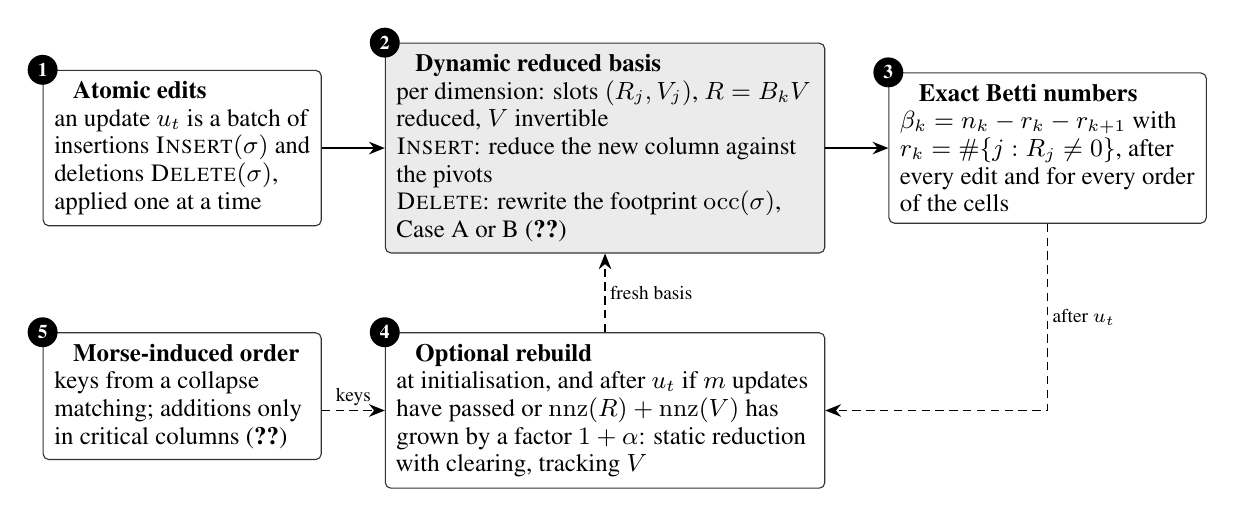
\begin{tikzpicture}[
    font=\footnotesize,
    >={Stealth[length=2mm,width=1.6mm]},
    part/.style={draw=black!80, rounded corners=2pt, fill=white, align=flush left,
      inner sep=4pt, text width=#1},
    core/.style={part=#1, fill=black!8},
    num/.style={circle, fill=black, text=white, inner sep=0pt, minimum size=3.8mm,
      font=\scriptsize\bfseries},
    flow/.style={->, semithick},
    rb/.style={->, semithick, dash pattern=on 3pt off 2pt},
    lbl/.style={font=\scriptsize, inner sep=1.5pt},
  ]
  % ----- update path ----------------------------------------------------------
  \node[part=3.25cm] (edits) at (0,0) {%
    \hspace*{2.4mm}\textbf{Atomic edits}\\
    an update $u_t$ is a batch of insertions $\Ins(\sigma)$ and deletions
    $\Del(\sigma)$, applied one at a time};
  \node[core=5.3cm, right=8mm of edits] (drb) {%
    \hspace*{2.4mm}\textbf{Dynamic reduced basis}\\
    per dimension: slots $(R_j,V_j)$, $R=\Bm{k}V$ reduced, $V$ invertible\\
    $\Ins$: reduce the new column against the pivots\\
    $\Del$: rewrite the footprint $\occ(\sigma)$, Case~A or~B
    (\cref{fig:deletion})};
  \node[part=3.75cm, right=8mm of drb] (betti) {%
    \hspace*{2.4mm}\textbf{Exact Betti numbers}\\
    $\beta_k=n_k-r_k-r_{k+1}$ with $r_k=\#\{j:R_j\ne0\}$, after every edit and
    for every order of the cells};
  % ----- rebuild path -----------------------------------------------------------
  \node[part=5.3cm, below=10mm of drb] (rebuild) {%
    \hspace*{2.4mm}\textbf{Optional rebuild}\\
    at initialisation, and after $u_t$ if $m$ updates have passed or
    $\nnz(R)+\nnz(V)$ has grown by a factor $1+\alpha$: static reduction with
    clearing, tracking $V$};
  \node[part=3.25cm, anchor=north east] (morse) at (edits.east |- rebuild.north) {%
    \hspace*{2.4mm}\textbf{Morse-induced order}\\
    keys from a collapse matching; additions only in critical columns
    (\cref{fig:morse})};
  % ----- numbers --------------------------------------------------------------
  \foreach \b/\n in {edits/1, drb/2, betti/3, rebuild/4, morse/5}
    \node[num] at (\b.north west) {\n};
  % ----- arrows ---------------------------------------------------------------
  \draw[flow] (edits) -- (drb);
  \draw[flow] (drb) -- (betti);
  \draw[rb] (betti.south) |- node[lbl, pos=0.25, right] {after $u_t$} (rebuild.east);
  \draw[rb] (morse.east |- rebuild.west) -- node[lbl, above] {keys} (rebuild.west);
  \draw[rb] (rebuild.north) -- node[lbl, right] {fresh basis} (drb.south);
\end{tikzpicture}

  \caption{The method. \emph{Top:} an update is processed one atomic edit at a
    time on the dynamic reduced basis of each boundary matrix
    (\cref{sec:drb}). An insertion reduces the new column against the pivots; a
    deletion rewrites every slot in the footprint $\occ(\sigma)$ of the deleted
    simplex, by a cycle (Case~A) or by the slot with the smallest low (Case~B).
    The Betti numbers are exact after every edit, whatever the order of the
    cells. \emph{Bottom, dashed:} a rebuild replaces the order by the Morse
    order of a collapse matching and recomputes the basis by the static
    reduction with clearing (\cref{sec:morse}). Under that order every gradient
    pair is an apparent pair and all column additions happen in columns of
    critical cells. Between rebuilds the Morse order is only a heuristic for
    sparsity (\cref{rem:morse-scope}). The ablations of \cref{sec:exp-methods}
    change the bottom path: \method{drb-id-rb} rebuilds in insertion order, and
    \method{drb-id} and \method{mmhm-norb} never rebuild.}
  \label{fig:method}
\end{figure}

% sections/drb.tex -- the dynamic reduced basis, its exactness (Theorem 1) and rebuilds (Proposition 1.1). Uses macros.tex. Executable checks of every statement:
% research/mmhm/reference/check_props.py.
\section{The dynamic reduced basis}\label{sec:drb}

Every cell $x\in K$ carries an \emph{order key} $\ord(x)$; keys of distinct cells
are distinct. For a non-zero chain $c$, $\low(c)$ is the cell of $c$ with the
largest key. Keys do not change between rebuilds (Section~\ref{sec:morse}); an
inserted cell receives a key larger than every key in use. Nothing in this
section depends on how the keys are chosen; \cref{sec:morse} chooses them.

\begin{definition}[DRB]\label{def:drb}
Let $k\ge1$. A \emph{dynamic reduced basis} of $\Bm{k}$ is a finite family of
\emph{slots} $j\in J_k$, each holding a pair $(R_j,V_j)$ with $V_j\in\Cc{k}$
and $R_j\in\Cc{k-1}$, such that
\begin{description}
\item[(I1)] $R_j=\bd_k V_j$ for every $j\in J_k$;
\item[(I2)] the non-zero $R_j$ have pairwise distinct lows;
\item[(I3)] $(V_j)_{j\in J_k}$ is a basis of $\Cc{k}$; in particular $|J_k|=n_k$.
\end{description}
Two index structures are derived from the slots: $\pivot(\ell)=j$ if $R_j\ne0$
and $\low(R_j)=\ell$ (well defined by (I2)), and, for $x\in\Kc{k}$,
$\occ(x)=\{j\in J_k : x\in V_j\}$, the \emph{footprint} of $x$. Both are updated
together with the chains; we do not spell out this bookkeeping.
\end{definition}

Writing $R$ and $V$ for the matrices with columns $R_j$ and $V_j$, (I1) and (I3)
say that $R=\Bm{k}V$ with $V$ invertible, and (I2) says that $R$ is
\emph{reduced}. Unlike the decomposition used for persistence, $V$ is not
required to be triangular with respect to $\ord$.

\paragraph{Insertion.} $\Ins(\sigma)$ for a $k$-simplex $\sigma\notin K$, $k\ge1$,
all of whose facets are in $K$:
\begin{enumerate}
\item give $\sigma$ a key larger than all keys in use; create a slot $j$ with
  $V_j=\{\sigma\}$ and $R_j=\bd\sigma$;
\item while $R_j\ne0$ and $p=\pivot(\low(R_j))$ is defined: $R_j\gets R_j+R_p$,
  $V_j\gets V_j+V_p$;
\item if $R_j\ne0$, set $\pivot(\low(R_j))=j$.
\end{enumerate}
The slots $p_1,\dots,p_m$ added in step~2 form the \emph{reduction chain} of
$\sigma$. We call $\sigma$ \emph{positive} if $R_j=0$ at the end and
\emph{negative} otherwise.

\paragraph{Deletion.} $\Del(\sigma)$ for $\sigma\in\Kc{k}$, $k\ge1$, without
cofaces. Let $O=\occ(\sigma)$ and $Z=\{j\in O: R_j=0\}$.
\begin{description}
\item[Case A ($Z\ne\emptyset$).] Choose any $z\in Z$ (the implementations take
  one with $|V_z|$ minimal, ties broken by the smallest slot index). For every $j\in O\setminus\{z\}$:
  $V_j\gets V_j+V_z$. Remove slot $z$.
\item[Case B ($Z=\emptyset$).] Let $p\in O$ be the slot whose $\low(R_p)$ has
  the smallest key. For every $j\in O\setminus\{p\}$: $R_j\gets R_j+R_p$ and
  $V_j\gets V_j+V_p$. Remove slot $p$ and the entry $\pivot(\low(R_p))$.
\end{description}
Finally remove $\sigma$ from $K$. Inserting or deleting a vertex changes only
$n_0$. \Cref{fig:deletion} carries out both cases on a graph.

\begin{figure}[t]
\centering
% figures/f2_deletion.tex -- the two deletion cases worked on graphs (k = 1).
% Rows of R are vertices with keys 0 < 1 < 2 < 3 (top to bottom, so the low of
% a column is its lowest non-zero entry); rows of V are edges; columns are slots.
% Every entry is computed and checked by reference/figure_examples.py.
\newcommand{\pv}[1]{{\setlength{\fboxsep}{0.6pt}\setlength{\fboxrule}{0.6pt}\fbox{$#1$}}}
\newcommand{\fc}{\cellcolor{black!14}}
\newcommand{\chg}[1]{\boldsymbol{#1}}
\tikzset{
  dvtx/.style={circle, draw=black!85, fill=white, inner sep=0pt, minimum size=3.6mm,
    font=\scriptsize},
  dedg/.style={black!80, semithick},
  dsig/.style={black, very thick, dash pattern=on 2.4pt off 1.5pt},
}
\newcommand{\whynote}[1]{{\scriptsize\raggedright #1\par}}
{\footnotesize\renewcommand{\arraystretch}{1.06}%
%
% =========================== (a) Case A ===================================
\begin{minipage}[t]{0.485\textwidth}
\textbf{(a) Case A:} $\sigma=01$ lies on a cycle\par\smallskip
\begin{tabular}{@{}c@{\hspace{0.7em}}l@{\hspace{1.1em}}l@{}}
\begin{tikzpicture}[baseline=(current bounding box.center)]
  \node[dvtx] (a0) at (0,0) {0}; \node[dvtx] (a1) at (1.1,0) {1};
  \node[dvtx] (a2) at (0.55,0.95) {2};
  \draw[dedg] (a0) -- (a2) (a1) -- (a2);
  \draw[dsig] (a0) -- node[below=-1pt, font=\scriptsize] {$\sigma$} (a1);
  \node[font=\scriptsize] at (0.55,-0.62) {$\beta=(1,1)$};
\end{tikzpicture}
& $V=\begin{array}{@{}r|ccc@{}}
    & s_1 & s_2 & s_3\\ \hline
    \fc 01 & \fc 1 & \fc 0 & \fc 1\\
    02 & 0 & 1 & 1\\
    12 & 0 & 0 & 1\end{array}$
& $R=\begin{array}{@{}r|ccc@{}}
    & s_1 & s_2 & s_3\\ \hline
    0 & 1 & 1 & 0\\
    1 & \pv{1} & 0 & 0\\
    2 & 0 & \pv{1} & 0\end{array}$\\[16pt]
$\Big\downarrow$ & \multicolumn{2}{@{}l@{}}{\parbox[c]{5.75cm}{\scriptsize\raggedright
    $O=\occ(\sigma)=\{s_1,s_3\}$ (the $1$s in the shaded row); $R_{s_3}=0$, so
    $Z=\{s_3\}$ and $z=s_3$.\\
    $V_{s_1}\gets V_{s_1}+V_{s_3}$; remove slot $s_3$ and row $\sigma$.}}\\[14pt]
\begin{tikzpicture}[baseline=(current bounding box.center)]
  \node[dvtx] (b0) at (0,0) {0}; \node[dvtx] (b1) at (1.1,0) {1};
  \node[dvtx] (b2) at (0.55,0.95) {2};
  \draw[dedg] (b0) -- (b2) (b1) -- (b2);
  \node[font=\scriptsize] at (0.55,-0.62) {$\beta=(1,0)$};
\end{tikzpicture}
& $V=\begin{array}{@{}r|cc@{}}
    & s_1 & s_2\\ \hline
    02 & \chg{1} & 1\\
    12 & \chg{1} & 0\end{array}$
& $R=\begin{array}{@{}r|cc@{}}
    & s_1 & s_2\\ \hline
    0 & 1 & 1\\
    1 & \pv{1} & 0\\
    2 & 0 & \pv{1}\end{array}$
\end{tabular}\par\medskip
\whynote{\textbf{Why a cycle.} $\bd V_{s_3}=R_{s_3}=0$, so the addition removes
  $\sigma$ from $V_{s_1}$ and leaves every $R_j$, hence every low, as it was.
  $n_1$ drops and $r_1=2$ stays: $\beta_1$ falls by one.}
\end{minipage}\hfill
%
% =========================== (b) Case B ===================================
\begin{minipage}[t]{0.485\textwidth}
\textbf{(b) Case B:} $\sigma=03$ lies on no cycle\par\smallskip
\begin{tabular}{@{}c@{\hspace{0.7em}}l@{\hspace{1.1em}}l@{}}
\begin{tikzpicture}[baseline=(current bounding box.center)]
  \node[dvtx] (c3) at (0.6,1.0) {3};
  \node[dvtx] (c0) at (0,0) {0}; \node[dvtx] (c1) at (0.6,0) {1};
  \node[dvtx] (c2) at (1.2,0) {2};
  \draw[dedg] (c1) -- (c3) (c2) -- (c3);
  \draw[dsig] (c0) -- node[left=-1pt, font=\scriptsize] {$\sigma$} (c3);
  \node[font=\scriptsize] at (0.6,-0.62) {$\beta=(1,0)$};
\end{tikzpicture}
& $V=\begin{array}{@{}r|ccc@{}}
    & s_1 & s_2 & s_3\\ \hline
    \fc 03 & \fc 1 & \fc 1 & \fc 1\\
    13 & 0 & 1 & 0\\
    23 & 0 & 0 & 1\end{array}$
& $R=\begin{array}{@{}r|ccc@{}}
    & s_1 & s_2 & s_3\\ \hline
    0 & 1 & 1 & 1\\
    1 & 0 & \pv{1} & 0\\
    2 & 0 & 0 & \pv{1}\\
    3 & \pv{1} & 0 & 0\end{array}$\\[16pt]
$\Big\downarrow$ & \multicolumn{2}{@{}l@{}}{\parbox[c]{5.75cm}{\scriptsize\raggedright
    $O=\{s_1,s_2,s_3\}$ and every $R_j\ne0$, so $Z=\emptyset$; the lows are
    $3,1,2$, and $p=s_2$ has the smallest.\\
    $(R_j,V_j)\gets(R_j+R_{s_2},V_j+V_{s_2})$ for $j=s_1,s_3$; remove slot $s_2$
    and row $\sigma$.}}\\[14pt]
\begin{tikzpicture}[baseline=(current bounding box.center)]
  \node[dvtx] (d3) at (0.6,1.0) {3};
  \node[dvtx] (d0) at (0,0) {0}; \node[dvtx] (d1) at (0.6,0) {1};
  \node[dvtx] (d2) at (1.2,0) {2};
  \draw[dedg] (d1) -- (d3) (d2) -- (d3);
  \node[font=\scriptsize] at (0.6,-0.62) {$\beta=(2,0)$};
\end{tikzpicture}
& $V=\begin{array}{@{}r|cc@{}}
    & s_1 & s_3\\ \hline
    13 & \chg{1} & \chg{1}\\
    23 & 0 & 1\end{array}$
& $R=\begin{array}{@{}r|cc@{}}
    & s_1 & s_3\\ \hline
    0 & \chg{0} & \chg{0}\\
    1 & \chg{1} & \chg{1}\\
    2 & 0 & \pv{1}\\
    3 & \pv{1} & 0\end{array}$
\end{tabular}\par\medskip
\whynote{\textbf{Why the smallest low.} Adding $R_{s_1}=\{0,3\}$, whose low $3$
  is the largest, would instead give $\{1,3\}$ and $\{2,3\}$: two lows $3$,
  violating (I2). $R_{s_2}$ lies entirely above the other lows, so adding it
  moves none. $n_1$ and $r_1$ both drop: $\beta_0$ rises by one.}
\end{minipage}}%

\caption{The two cases of $\Del(\sigma)$, worked on graphs ($k=1$). Columns are
slots. The rows of $V$ are edges; the rows of $R$ are vertices in key order from
top to bottom, so the low of a column is its lowest non-zero entry (boxed). The
shaded row of $V$ is $\sigma$, and its $1$s mark the footprint $O$. Bold entries
are those changed by the update; $\beta=(\beta_0,\beta_1)$.
(a)~A footprint slot is a cycle ($R_{s_3}=0$); adding it to the other footprint
slot clears $\sigma$ from $V$ and leaves $R$ unchanged.
(b)~No footprint slot is a cycle; the slot with the smallest low is added to the
others and removed, and no low moves.
Every entry is recomputed and checked by \texttt{reference/figure\_examples.py}.}
\label{fig:deletion}
\end{figure}

\begin{theorem}[Exactness]\label{thm:exact}
Let $k\ge1$ and let $(R_j,V_j)_{j\in J_k}$ satisfy (I1)--(I3) for $\Bm{k}(K)$,
for some injective key function.
\begin{enumerate}
\item[(a)] $r_k=\#\{j\in J_k : R_j\ne0\}$, and $\{V_j : R_j=0\}$ is a basis of
  $\Zc{k}(K)$.
\item[(b)] Let $\sigma\notin K$ be a $k$-simplex whose facets are all in $K$.
  The loop of $\Ins(\sigma)$
  terminates, and afterwards the slots satisfy (I1)--(I3) for
  $\Bm{k}(K\cup\{\sigma\})$; every family satisfying (I1)--(I3) for
  $\Bm{k+1}(K)$ satisfies them, unchanged, for $\Bm{k+1}(K\cup\{\sigma\})$.
\item[(c)] Let $\sigma\in\Kc{k}$ have no coface. Then $O\ne\emptyset$; after
  $\Del(\sigma)$, in Case A and in Case B, the slots satisfy (I1)--(I3) for
  $\Bm{k}(K\setminus\{\sigma\})$; every family satisfying (I1)--(I3) for
  $\Bm{k+1}(K)$ satisfies them, unchanged, for $\Bm{k+1}(K\setminus\{\sigma\})$.
\item[(d)] Inserting a positive $k$-simplex increases $\beta_k$ by one; inserting
  a negative one decreases $\beta_{k-1}$ by one. A deletion in Case A decreases
  $\beta_k$ by one; a deletion in Case B increases $\beta_{k-1}$ by one. No
  other Betti number changes. Moreover, $\Del(\sigma)$ is in Case A if and only
  if $\sigma$ lies in the support of a $k$-cycle of $K$, and $\Ins(\sigma)$ is
  positive if and only if $\sigma$ lies in the support of a $k$-cycle of
  $K\cup\{\sigma\}$.
\end{enumerate}
\end{theorem}

\begin{proof}
(a) By (I1) and (I3), $R=\Bm{k}V$ with $V$ invertible, so $\rank R=r_k$. The
non-zero columns of $R$ are linearly independent: in a non-empty sum of them,
let $R_i$ be the summand whose low $\ell$ has the largest key; every other
summand has its low, hence all its cells, strictly below $\ell$, so $\ell$
survives in the sum. Hence $r_k$ is the number of non-zero $R_j$. Each $V_j$ with
$R_j=0$ is a cycle; these chains are independent as part of a basis, and there
are $n_k-r_k=\dim\Zc{k}$ of them.

(b) Let $K'=K\cup\{\sigma\}$. Throughout the loop, $R_j=\bd V_j$ (true at the
start and preserved by linearity because $R_p=\bd V_p$) and $V_j=\sigma+w$ with
$w\in\Cc{k}(K)$. An addition is performed only when $\low(R_p)=\low(R_j)=\ell$;
all cells of both chains have keys at most $\ord(\ell)$ and $\ell$ cancels, so
afterwards $R_j=0$ or $\low(R_j)$ is strictly smaller. Hence the loop
terminates, after at most one addition per non-zero slot. On exit either
$R_j=0$ or $\low(R_j)$ is no pivot, so recording the pivot preserves (I2); (I1)
holds. Since $\Cc{k}(K')=\Cc{k}(K)\oplus\Z\sigma$ and the old $V_i$ form a basis
of $\Cc{k}(K)$, the old chains together with $V_j=\sigma+w$ form a basis of
$\Cc{k}(K')$: they are $n_k+1$ chains spanning $\sigma=V_j+w$. For $\Bm{k+1}$:
the chain group $\Cc{k+1}$ is unchanged, each $R_i=\bd V_i$ is supported on facets
of $(k+1)$-simplices of $K'$, none of which is $\sigma$
(Observation~\ref{obs:structural}), and keys of existing cells are unchanged;
so (I1)--(I3) continue to hold.

(c) Since the $V_j$ span $\Cc{k}$, $\sigma$ is a sum of some of them, so some
$V_j$ contains $\sigma$: $O\ne\emptyset$. Each operation $V_j\gets V_j+V_q$ with
$j\ne q$ is an invertible change of basis, so throughout the loop the family
remains a basis of $\Cc{k}(K)$. For $j\in O\setminus\{q\}$ (with $q=z$ in Case A,
$q=p$ in Case B), both $V_j$ and $V_q$ contain $\sigma$, so $V_j+V_q$ does not;
slots outside $O$ never contained $\sigma$. After the loop, $V_q$ is therefore
the only chain containing $\sigma$. Removing slot $q$ leaves $n_k-1$ independent
chains, all in $\Cc{k}(K\setminus\{\sigma\})$, which has dimension $n_k-1$:
(I3) holds.
\emph{Case A.} Because $\bd V_z=R_z=0$, the additions leave every $R_j$
unchanged, so (I1) and (I2) hold; the removed slot had $R_z=0$ and owned no
pivot.
\emph{Case B.} Every $R_j$ with $j\in O$ is non-zero, and by (I2) the lows are
distinct, so $p$ is well defined and $\low(R_p)$ is strictly smaller than
$\low(R_j)$ for $j\in O\setminus\{p\}$. All cells of $R_p$ have keys at most
$\ord(\low(R_p))<\ord(\low(R_j))$, so $\low(R_j)\notin R_p$ and
$\low(R_j+R_p)=\low(R_j)$; in particular $R_j+R_p\ne0$. Lows are unchanged and
the low of $R_p$ is released with slot $p$, so (I2) holds; (I1) holds by
linearity. (The minimal choice of $p$ is what guarantees this: adding an $R_p$
with a larger low would move lows and require further reduction.)
For $\Bm{k+1}$: $\sigma$ has no coface, so no $R_i=\bd V_i$ of dimension $k+1$
contains $\sigma$ and $\sigma$ is not a pivot there; deleting the zero row
$\sigma$ leaves (I1)--(I3) intact.

(d) By (a), $r_k$ increases by one exactly when the inserted $\sigma$ is negative,
and decreases by one exactly in Case B; $n_k$ changes by $\pm1$; $r_{k+1}$ is
unchanged because only a zero row of $\Bm{k+1}$ is added or removed
(Observation~\ref{obs:structural}); all other $n_i$ and $r_i$ are unchanged.
Formula~\eqref{eq:betti} gives the stated changes. If
$z\in Z$, then $V_z$ is a cycle containing $\sigma$. Conversely, if a cycle
$c\in\Zc{k}(K)$ contains $\sigma$, write $c$ in the basis
$\{V_j:R_j=0\}$ of $\Zc{k}(K)$ from (a); some $V_j$ in this expansion contains
$\sigma$, and that $j$ lies in $Z$. For insertion, if $\sigma$ is positive then
the final $V_j$ is a cycle of $K'$ containing $\sigma$. Conversely, if a cycle
$c$ of $K'$ contains $\sigma$, then $\bd\sigma=\bd(c+\sigma)$ lies in the
column space of $\Bm{k}(K)$, so $r_k$ does not increase, and by (a) the new slot
has $R_j=0$.
\end{proof}

Vertices need no slots: inserting a vertex increases $n_0$ and $\beta_0$ by
one, and a deletable vertex is isolated, so deleting it decreases both by one
(Observation~\ref{obs:structural} and~\eqref{eq:betti}). A batch is processed
one atomic edit at a time, so Theorem~\ref{thm:exact} makes the Betti numbers
exact after every update. The choice of $z$ in Case A
is free; it only affects sparsity. Theorem~\ref{thm:exact} holds for every key
function, so the order chosen in Section~\ref{sec:morse} is a matter of cost
alone.

\paragraph{Initialisation and rebuilds.}
The DRB is initialised, and periodically rebuilt, by the static reduction with
clearing~\cite{chen2011twist}, tracking $V$: for $k=d,d-1,\dots,1$, process the
columns of $\Bm{k}$ in increasing key order; if the $k$-simplex $\tau$ is the low
of a non-zero reduced column $R$ of $\Bm{k+1}$, \emph{clear} it ($R_\tau:=0$,
$V_\tau:=R$); otherwise reduce it as in steps~2--3 of $\Ins$, starting from
$V_\tau=\{\tau\}$, $R_\tau=\bd\tau$.

\begin{subproposition}[Rebuild]\label{cor:rebuild}
For every injective key function, the static reduction with clearing produces
slots satisfying (I1)--(I3) in every dimension. Moreover, every $V_\tau$ consists
of $\tau$ and cells with smaller keys. The same holds for the reduction without
clearing. In particular the ranks it reports are exact even when $V$ is not
stored.
\end{subproposition}

\begin{proof}
We show $\low(V_\tau)=\tau$ for every column $\tau$, by induction along the
processing order. A non-cleared $\tau$ ends with
$V_\tau=\{\tau\}+\sum V_p$ over pivot owners $p$ processed earlier, hence with
smaller keys, and by induction every cell of $V_p$ has key at most $\ord(p)$. A
cleared $\tau$ has $V_\tau=R$ with $\low(R)=\tau$. Ordering rows and columns by
key, $V$ is therefore upper unitriangular, hence invertible: (I3). (I1) holds
for non-cleared columns by linearity, and for cleared ones because $R=\bd V'$
for the slot $V'$ of $\Bm{k+1}$ that produced it (induction over dimensions), so
$\bd V_\tau=\bd\bd V'=0=R_\tau$. (I2): a non-cleared column ends with $R_\tau=0$ or
with a low that no earlier column owns; cleared columns are zero. Without
clearing every column is of the non-cleared kind and the same argument applies.
The last statement follows from Theorem~\ref{thm:exact}(a).
\end{proof}

Note that the correctness of clearing here follows from the invariants alone;
we do not need the classical fact that a cleared column would have reduced to
zero. After deletions, however, $V$ is no longer triangular (Case A adds
$V_z$, whose low may exceed that of $V_j$), so the DRB maintains ranks and a cycle
basis but not a persistence pairing, and we claim none. This is the difference
from vineyard updates~\cite{cohensteiner2006vines}, which keep $V$ triangular
for a changing order.

\paragraph{Rebuild policy.} \method{mmhm} rebuilds with the Morse order of Section~\ref{sec:morse}; it
rebuilds after update $t$ if $t-t_{\mathrm{last}}\ge m$ or
$\nnz(R)+\nnz(V)>(1+\alpha)\max(\nnz_{\mathrm{last}},|K|)$, where
$\nnz_{\mathrm{last}}$ is the value right after the previous rebuild (defaults
$m=\infty$, $\alpha=1$), and the rebuild is charged to update $t$.
\method{drb-id} uses insertion keys and never rebuilds; \method{mmhm-norb} uses
the Morse order at the initial build only; \method{drb-id-rb} applies the same
policy as \method{mmhm} but rebuilds in insertion order
(Section~\ref{sec:exp-methods}).

% sections/morse.tex -- the Morse order: Lemma 2 and Corollaries 2.1--2.2. Uses macros.tex. Executable checks of every statement:
% research/mmhm/reference/check_props.py.
\section{The Morse order}\label{sec:morse}

Discrete Morse theory~\cite{forman2002user} enters only through the choice of
keys at a rebuild. A rebuild computes an acyclic matching by collapses, in the
spirit of~\cite{benedetti2014random}, and orders cells by reverse removal time.

\begin{definition}[Collapse matching and Morse order]\label{def:collapse}
Run the following on $P:=K$, with a counter $t:=0$ and a queue $Q$ of the cells
$x$ that have exactly one immediate coface in $P$ (\emph{free faces}).
\begin{enumerate}
\item While $Q\ne\emptyset$: pop $x$; skip it unless $x\in P$ and $x$ has
  exactly one immediate coface $y$ in $P$. Then \emph{pair} $(x,y)$, set
  $\rmt(y):=t$, $\rmt(x):=t+1$, $t\gets t+2$, remove $y$ and $x$ from $P$, and
  push every facet of $y$ or $x$ that has become free.
\item If $P\ne\emptyset$, choose a cell $c$ of the highest dimension present in
  $P$ (smallest vertex tuple), declare it \emph{critical}, set $\rmt(c):=t$,
  $t\gets t+1$, remove it, push the facets that have become free, and go to~1.
\end{enumerate}
The \emph{Morse order} is $\ord(x):=-\rmt(x)$ (relabelled to $0,\dots,|K|-1$).
Write $M$ for the set of pairs, $\Crit$ for the critical cells, $\Lo$ for the
cells $x$ with $(x,y)\in M$ and $\Up$ for the cells $y$ with $(x,y)\in M$; for
$x\in\Lo$ let $\mu(x)$ be its partner. For a cell $x$, its \emph{youngest facet}
is the facet with the largest key and its \emph{oldest coface} the coface with
the smallest key.
\end{definition}

The removed cells are always maximal in $P$, and $P$ remains a subcomplex. For
the paired cell $y$ this uses the simplicial diamond property: if $y$ had a
coface $w\in P$, then $w$ would have exactly two facets containing $x$, namely
$y$ and some $y'\ne y$, and $y'\in P$ because $P$ is a subcomplex, so $x$ would
not be free. The queue discipline is not specified; all results below hold for
every discipline. \Cref{fig:morse} runs the procedure on a small complex.

A \emph{gradient path} (V-path) is a sequence $\tau_0,\sigma_0,\tau_1,\sigma_1,
\dots,\tau_m$ with $(\tau_i,\sigma_i)\in M$ and $\tau_{i+1}$ a facet of
$\sigma_i$ different from $\tau_i$.

\begin{lemma}[Gradient pairs are apparent pairs]\label{lem:apparent}
For every execution of the collapse procedure, with $\ord=-\rmt$:
\begin{enumerate}
\item[(a)] $\ord$ is a filtration order: $\ord(f)<\ord(s)$ whenever $f$ is a facet
  of $s$.
\item[(b)] $\rmt$ strictly increases along the lower cells of every gradient
  path ($\rmt(\tau_{i+1})>\rmt(\tau_i)$); in particular $M$ has no closed
  gradient path, so it is an acyclic matching.
\item[(c)] For every $(\tau,\sigma)\in M$: $\tau$ is the youngest facet of
  $\sigma$, i.e.\ $\tau=\low(\bd\sigma)$, and $\sigma$ is the oldest coface of
  $\tau$.
\item[(d)] If $z\ne0$ is a cycle, then $\low(z)\notin\Up$.
\item[(e)] In the static reduction under $\ord$, with or without clearing, for
  every $(\tau,\sigma)\in M$ the column $\sigma$ is not cleared, receives no
  addition, and obtains pivot $\tau$; thus $R_\sigma=\bd\sigma$ and
  $(\tau,\sigma)$ is an \emph{apparent pair}~\cite{bauer2021ripser}.
\end{enumerate}
\end{lemma}

\begin{proof}
(a) Only maximal cells of $P$ are removed (above), so every cell is removed
before each of its facets.

(b) When $\sigma_i$ is removed at time $\rmt(\sigma_i)$, its facet $\tau_{i+1}$ is
still in $P$. Times $\rmt(\sigma_i)$ and $\rmt(\tau_i)=\rmt(\sigma_i)+1$ are
used by $\sigma_i$ and $\tau_i$, and $\tau_{i+1}\ne\tau_i$, so
$\rmt(\tau_{i+1})>\rmt(\tau_i)$. A closed gradient path would give
$\rmt(\tau_0)<\rmt(\tau_0)$.

(c) The pair is removed at consecutive times, so $\ord(\tau)=\ord(\sigma)-1$:
the two cells are adjacent in the order. By (a) every facet of $\sigma$ precedes
$\sigma$, hence has key at most $\ord(\tau)$, and every coface of $\tau$ follows
$\tau$, hence has key at least $\ord(\sigma)$. (This is the elementary fact that
a facet and a coface that are adjacent in a filtration order form an apparent
pair.)

(d) Let $u=\low(z)\in\Up$ with $u=\mu(w)$. The coefficient of $w$ in $\bd z=0$
vanishes and $w\in\bd u$, so some $u'\in z$ with $u'\ne u$ has $w$ as a facet.
By (c), $u$ is the oldest coface of $w$, so $\ord(u')>\ord(u)$, contradicting
$u=\low(z)$.

(e) If $\sigma$ were cleared, it would be the low of a reduced column $R$ of the
next dimension; $R=\bd V'$ (Proposition~\ref{cor:rebuild}) is a non-zero cycle with
low $\sigma\in\Up$, contradicting (d). Columns are processed in increasing key
order. When $\sigma$ is processed, every earlier column $x$ has $R_x=0$ (if
cleared) or $R_x=\bd V_x$ with all cells of $V_x$ of key at most
$\ord(x)<\ord(\sigma)$ (Proposition~\ref{cor:rebuild}); by (c) no such cell has
$\tau$ as a facet, so $\tau\notin R_x$ and $\pivot(\tau)$ is undefined. Since
$\low(\bd\sigma)=\tau$ by (c), the reduction loop performs no addition and
assigns $\pivot(\tau)=\sigma$.
\end{proof}

\begin{corollary}[Work happens only on critical columns]\label{cor:critical-work}
In the static reduction with clearing under the Morse order, the column of every
$x\in\Lo$ with $\dim x\ge1$ is cleared, the column of every $y\in\Up$ is
apparent, and therefore every column addition is performed while reducing the
column of a critical cell.
\end{corollary}

\begin{proof}
For $(x,y)\in M$ with $\dim y=k+1\ge2$, Lemma~\ref{lem:apparent}(e) applied to
$\Bm{k+1}$, which is processed before $\Bm{k}$, gives $R_y=\bd y$ with
$\low(R_y)=x$, so $x$ is cleared. Upper cells are apparent by
Lemma~\ref{lem:apparent}(e). Every remaining column belongs to a critical cell.
\end{proof}

\begin{figure}[t]
\centering
% figures/f3_morse.tex -- the Morse order on a small complex: collapse, gradient
% pairs, critical cells, apparent pairs in the boundary matrices, and the
% reduction of the critical column. Rows and columns of every matrix are in key
% order (rows top to bottom), so a low is the lowest non-zero entry.
% Every entry is computed and checked by reference/figure_examples.py.
\newcommand{\pv}[1]{{\setlength{\fboxsep}{0.6pt}\setlength{\fboxrule}{0.6pt}\fbox{$#1$}}}
\newcommand{\cc}{\cellcolor{black!14}}
\newcommand{\gz}[1]{\textcolor{black!40}{#1}}
{\footnotesize\renewcommand{\arraystretch}{1.06}%
%
% ====================== (a) complex and matching ==========================
\begin{minipage}[t]{0.29\textwidth}
\textbf{(a)} Complex, matching, critical cells\par\medskip
\centering
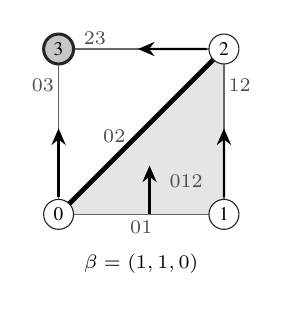
\begin{tikzpicture}[>={Stealth[length=2.1mm,width=1.8mm]},
    mvtx/.style={circle, draw=black!85, fill=white, inner sep=0pt, minimum size=3.8mm,
      font=\scriptsize},
    cvtx/.style={mvtx, fill=black!22, line width=1.1pt},
    medg/.style={black!60, semithick},
    cedg/.style={black, line width=1.7pt},
    pair/.style={->, black, thick},
    lab/.style={font=\scriptsize, text=black!70, inner sep=1.5pt}]
  \coordinate (p0) at (0,0);     \coordinate (p1) at (2.1,0);
  \coordinate (p2) at (2.1,2.1); \coordinate (p3) at (0,2.1);
  \fill[black!10] (p0) -- (p1) -- (p2) -- cycle;
  \draw[medg] (p0) -- (p1) -- (p2) -- (p3) -- cycle;
  \draw[cedg] (p0) -- (p2);
  \draw[pair] ($(p0)+(0,0.22)$) -- ($(p0)!0.52!(p3)$);
  \draw[pair] ($(p1)+(0,0.22)$) -- ($(p1)!0.52!(p2)$);
  \draw[pair] ($(p2)+(-0.22,0)$) -- ($(p2)!0.52!(p3)$);
  \draw[pair] ($(p0)!0.55!(p1)$) -- ++(0,0.62);
  \node[mvtx] at (p0) {0}; \node[mvtx] at (p1) {1};
  \node[mvtx] at (p2) {2}; \node[cvtx] at (p3) {3};
  \node[lab, below] at ($(p0)!0.5!(p1)+(0,-0.02)$) {$01$};
  \node[lab, right] at ($(p1)!0.78!(p2)$) {$12$};
  \node[lab, above] at ($(p2)!0.78!(p3)$) {$23$};
  \node[lab, left] at ($(p0)!0.78!(p3)$) {$03$};
  \node[lab, above left=-1pt] at ($(p0)!0.42!(p2)$) {$02$};
  \node[lab] at (1.62,0.42) {$012$};
  \node[font=\scriptsize] at (1.05,-0.62) {$\beta=(1,1,0)$};
\end{tikzpicture}
\end{minipage}\hfill
%
% ====================== (b) collapse and order ============================
\begin{minipage}[t]{0.68\textwidth}
\textbf{(b)} Collapse and Morse order\par\medskip
{\scriptsize Collapse steps: pair $(01,012)$, pair $(1,12)$; no free face is left,
so $02$ is critical; pair $(2,23)$, pair $(0,03)$; $3$ is critical.}\par\smallskip
\begin{tabular}{@{}r@{\hspace{0.9em}}*{10}{c}@{}}
cell & $\mathbf{3}$ & $0$ & $03$ & $2$ & $23$ & $\mathbf{02}$ & $1$ & $12$ & $01$ & $012$\\
\cmidrule(lr){3-4}\cmidrule(lr){5-6}\cmidrule(lr){8-9}\cmidrule(lr){10-11}
& crit. & \multicolumn{2}{c}{pair} & \multicolumn{2}{c}{pair} & crit.
  & \multicolumn{2}{c}{pair} & \multicolumn{2}{c}{pair}\\[3pt]
key $\ord$ & 0 & 1 & 2 & 3 & 4 & 5 & 6 & 7 & 8 & 9\\
removal time $\rmt$ & 9 & 8 & 7 & 6 & 5 & 4 & 3 & 2 & 1 & 0
\end{tabular}
\end{minipage}

\bigskip
%
% ====================== (c) boundary matrices =============================
\begin{minipage}[t]{0.5\textwidth}
\textbf{(c)} Boundary matrices in the Morse order\par\medskip
\centering
$B_2=\begin{array}{@{}r|c@{}}
    & 012\\ \hline
    03 & 0\\
    23 & 0\\
    02 & 1\\
    12 & 1\\
    01 & \pv{1}\end{array}$\qquad
$B_1=\begin{array}{@{}r|ccccc@{}}
    & 03 & 23 & \cc 02 & 12 & \gz{01}\\ \hline
    3 & 1 & 1 & \cc 0 & 0 & \gz{0}\\
    0 & \pv{1} & 0 & \cc 1 & 0 & \gz{1}\\
    2 & 0 & \pv{1} & \cc 1 & 1 & \gz{0}\\
    1 & 0 & 0 & \cc 0 & \pv{1} & \gz{1}\end{array}$\par\smallskip
\raggedright{\scriptsize Boxed: the apparent pivots, $R_y=\bd y$ with low
$x$ for $(x,y)\in M$. Column $01$ (grey) is cleared, since $01$ is the low of
$R_{012}$. Only the shaded critical column $02$ is reduced
(\cref{cor:critical-work}).}
\end{minipage}\hfill
%
% ====================== (d) reduction of the critical column ===============
\begin{minipage}[t]{0.46\textwidth}
\textbf{(d)} Reducing the critical column $02$\par\medskip
\centering
$\begin{array}{@{}r|c@{}}
    & \bd 02\\ \hline
    3 & 0\\
    0 & 1\\
    2 & \pv{1}\\
    1 & 0\end{array}
\xrightarrow{\;\mu(2)=23\;}
\begin{array}{@{}c@{}}
    {+}\bd 23\\ \hline
    1\\
    \pv{1}\\
    0\\
    0\end{array}
\xrightarrow{\;\mu(0)=03\;}
\begin{array}{@{}c@{}}
    {+}\bd 03\\ \hline
    0\\
    0\\
    0\\
    0\end{array}$\par\smallskip
\raggedright{\scriptsize Each addition replaces the low, a lower cell, by the
other facet of its partner, following the gradient paths $2\to23\to3$ and
$0\to03\to3$ (\cref{cor:morse-reduction}). The column ends at
$\dM 02=3+3=0$: $V_{02}=02+23+03$ is the cycle around the empty triangle, so
$02$ is positive.}
\end{minipage}}%

\caption{The Morse order on a small complex $K$: the square $0123$ with
diagonal $02$ and the triangle $012$ (shaded); the triangle $023$ is not in $K$.
(a)~Arrows point from $x$ to $\mu(x)$ for the gradient pairs found by the
collapse; the critical cells $3$ and $02$ are drawn heavy.
(b)~Reading the removal times from right to left replays the collapse; the keys
are $\ord=9-\rmt$. Each pair is adjacent in the order and its lower cell is the
youngest facet of its partner, so each pair is apparent (\cref{lem:apparent}).
(c)--(d)~Rows and columns are in key order, rows from top to bottom, so a low is
the lowest non-zero entry (boxed).
Every entry is recomputed and checked by \texttt{reference/figure\_examples.py}.}
\label{fig:morse}
\end{figure}

\paragraph{Morse boundary.} By Lemma~\ref{lem:apparent}(b) the following
recursion is well founded and defines a linear map
$\flow\colon\Cc{k-1}\to\Cc{k-1}$: $\flow(\tau)=\tau$ for $\tau\in\Crit$,
$\flow(\tau)=0$ for $\tau\in\Up$, and
$\flow(\tau)=\sum_{\tau'\in\bd\mu(\tau),\,\tau'\ne\tau}\flow(\tau')$ for
$\tau\in\Lo$. Thus $\flow(\tau)$ is the sum, over all gradient paths from $\tau$
to a critical cell, of their endpoints, counted mod~2. The \emph{Morse boundary}
of a critical $k$-cell $c$ is $\dM c:=\flow(\bd c)$, the boundary of the Morse
complex of the matching~\cite{forman2002user}; the Morse boundary matrices
$\Bm{k}^M$ have rows $\Crit\cap\Kc{k-1}$ and columns $\Crit\cap\Kc{k}$. For
$y\in\Up$ with partner $x$, the definition of $\flow(x)$ gives
\begin{equation}\label{eq:flow-kills}
  \flow(\bd y)=\flow(x)+\sum_{f\in\bd y,\,f\ne x}\flow(f)=0 .
\end{equation}

\begin{corollary}[Critical columns perform the Morse reduction]\label{cor:morse-reduction}
Consider the static reduction with clearing under the Morse order and, next to
it, the standard reduction with clearing of the Morse boundary matrices
$\Bm{d}^M,\dots,\Bm{1}^M$, critical cells taken in increasing key order. For
every critical $k$-cell $c$, $k\ge1$:
\begin{enumerate}
\item[(i)] the additions performed on column $c$ are first additions of apparent
  columns $R_y=\bd y$ ($y\in\Up$), then additions of columns of critical cells;
\item[(ii)] if $c$ is not cleared, then when the first phase ends the column
  contains no cell of $\Lo$ and its restriction to $\Crit$ equals $\dM c$;
\item[(iii)] the second phase performs, one for one, the additions that the
  Morse reduction performs on column $c$; $c$ is cleared exactly when it is
  cleared in the Morse reduction; and the final column $R_c$ contains no cell
  of $\Lo$, while $R_c\cap\Crit$ is the reduced Morse column of $c$.
\end{enumerate}
\end{corollary}

Each first-phase addition $R\gets R+\bd y$ with $\low(R)=x$ and $y=\mu(x)$
replaces $x$ by the other facets of $y$; it is one step of the discrete gradient
flow, and $\flow(R)$ does not change by~\eqref{eq:flow-kills}. This is the
precise sense in which the reduced column of a critical cell ``traces its
gradient flow'' (\cref{fig:morse}d). $R_c$ may still contain cells of $\Up$; we observed this in
the randomised checks and claim nothing about them.

\begin{proof}
We use the rule of Definition~\ref{def:collapse} that a critical cell is chosen
of the highest dimension present in $P$. (Lemma~\ref{lem:apparent} did not use
it.)

\emph{Claim (separation).} For every $q$, every critical $q$-cell has a smaller
key than every $q$-cell of $\Lo$. Indeed, when a critical $q$-cell $t$ is removed,
$P$ contains no $(q+1)$-cell. If $\ell\in\Lo$ were a $q$-cell with
$\rmt(\ell)>\rmt(t)$, its partner $\mu(\ell)$, a $(q+1)$-cell removed at time
$\rmt(\ell)-1\ge\rmt(t)$, would be in $P$ at that moment.

We argue by induction over the dimensions (top-down) and, within $\Bm{k}$, over
the columns in increasing key order. The statement about clearing is shown below;
a cleared column receives no addition and has $R_c=0$, matching the zero column
of the Morse reduction. So let $c$ be a column that is not cleared, and let $R$
denote its column during its reduction; initially $R=\bd c$.

\emph{First phase.} Suppose $\ell=\low(R)\in\Lo$ and let $y=\mu(\ell)$. All cells
added to $V_c$ so far are $c$ and upper cells with smaller keys, so $\ell$ is a
facet of a cell $x$ with $\ord(x)\le\ord(c)$; since $y$ is the oldest coface of
$\ell$ (Lemma~\ref{lem:apparent}(c)) and $y\ne c$, $\ord(y)<\ord(c)$. By
Lemma~\ref{lem:apparent}(e), the column of $y$ has been processed, holds
$R_y=\bd y$ and owns $\pivot(\ell)$; the algorithm adds it, which
strictly decreases the low and preserves $\flow(R)$ by~\eqref{eq:flow-kills}.
The phase ends with $R=0$ or with $t=\low(R)\notin\Lo$. In the latter case $R$
is a non-zero cycle (by (I1), $R=\bd V_c$), so $t\notin\Up$ by
Lemma~\ref{lem:apparent}(d), and $t\in\Crit$. By the separation claim every
cell of $R$, having key at most $\ord(t)$, lies outside $\Lo$. As $\flow$ fixes
critical cells and kills upper cells,
$R\cap\Crit=\flow(R)=\flow(\bd c)=\dM c$. This proves (ii) and the first part
of (i).

\emph{Clearing.} The cells cleared in $\Bm{k}$ are the lows of the non-zero
reduced columns of $\Bm{k+1}$: the lower cells (lows of apparent columns) and
the lows of non-zero critical columns. By the induction hypothesis (iii) for
dimension $k+1$, the latter are critical and coincide with the lows of the
non-zero reduced Morse columns, i.e.\ with the cells cleared in the Morse
reduction. So a critical $c$ is cleared in one reduction if and only if in the
other; in the top dimension nothing is cleared in either.

\emph{Second phase.} A pivot on a critical row cannot be owned by an apparent
column (its low is in $\Lo$) or a cleared one (zero), so it is owned by a
critical column $c'$ processed earlier. By the induction hypothesis $R_{c'}$ has
no cell of $\Lo$, it is a cycle, its low is critical and equals
$\low(R_{c'}\cap\Crit)$, and $R_{c'}\cap\Crit$ is the reduced Morse column of
$c'$; hence the pivot tables of the two reductions agree on critical rows.
Adding such columns keeps $R\cap\Lo=\emptyset$ and keeps $R$ a cycle, so while
$R\ne0$ its low is critical and equals $\low(R\cap\Crit)$. The sequence of pivot
look-ups and additions on $R\cap\Crit$, which starts from $\dM c$, is therefore
exactly the Morse reduction of column $c$, and no apparent column is added any
more. This proves (i) and (iii).
\end{proof}

\begin{remark}[Relation to known results]\label{rem:morse-literature}
Lemma~\ref{lem:apparent} is not new in substance. Its part~(c) is the
elementary fact noted in its proof, and the relation between gradient pairs and
apparent pairs is known in both directions: the apparent pairs of any
simplexwise filtration form a discrete gradient, which Ripser uses to skip
columns~\cite{bauer2021ripser}, and Bauer and Roll~\cite{bauer2024wrapping}
relate the gradient pairs of a (generalised) discrete Morse function to the
zero-persistence apparent pairs of a lexicographically refined filtration
order. Lemma~\ref{lem:apparent} is a self-contained version for the order
produced by our collapse procedure, in the form used below: for every queue
discipline, with and without clearing, and with part~(d), on which
Corollary~\ref{cor:morse-reduction} rests. Mischaikow and Nanda~\cite{mischaikow2013morse} showed that
Morse reductions compatible with a filtration preserve persistent homology;
Corollary~\ref{cor:morse-reduction} is a matrix-level form of this for our order:
on critical rows and columns, the static reduction \emph{is} the reduction of
the Morse complex, and by Corollary~\ref{cor:critical-work} the other columns
cost no additions. This is what the \method{full-morse} baseline exploits. In the
language of algebraic Morse theory~\cite{skoldberg2006morse,jollenbeck2009minimal},
the first phase of
Corollary~\ref{cor:morse-reduction} is Gaussian elimination of the invertible
entries $\langle\bd y,x\rangle=1$ of the matched pairs, which is how the Morse
complex arises algebraically; the order makes the reduction algorithm perform
these eliminations by itself, without a separate Morse-reduction pass.
\end{remark}

\begin{remark}[Scope]\label{rem:morse-scope}
Lemma~\ref{lem:apparent} and its corollaries describe the state produced by a
rebuild. Between rebuilds the matching is not maintained, inserted cells get
keys larger than all others, and deletions add chains whose lows may exceed
those of their targets. We make no claim that the DRB stays sparse between
rebuilds; the Morse order is a heuristic for small footprints and short
reduction chains, its effect is measured, and the rebuild policy bounds the
drift of $\nnz(R)+\nnz(V)$.
\end{remark}

% sections/cost.tex -- update cost (Proposition 3) and the limits of locality (Proposition 4). Uses macros.tex. Executable checks of every statement:
% research/mmhm/reference/check_props.py.
\section{Update cost and the limits of locality}\label{sec:cost-locality}

\subsection{Output-sensitive cost}\label{sec:cost}

We state the cost in two storage models. In the \emph{ordered-set model}, a
chain is a balanced search tree keyed by $\ord$ and a footprint is a set of
slots; inserting, removing or testing one cell or slot, one pivot-table
operation and one low query are \emph{elementary operations}, each of
$O(\log n)$ time, $n=|K|$. In the \emph{sorted-array model}, which is what the
engine implements (Section~\ref{sec:exp-platform}), a chain is an increasing
array of keys, its low is its last entry, and a sum $x+y$ of two chains is a
linear merge that costs $\Theta(|x|+|y|)$, the size of the target included.
For an insertion we write $R^{(i)}$ and $V^{(i)}$ for the working column just
before the $i$-th addition of its reduction chain.

\begin{proposition}[Output-sensitive cost]\label{prop:cost}
Let $\sigma$ be a $k$-simplex, $k\ge1$.
\begin{enumerate}
\item[(a)] $\Ins(\sigma)$ with reduction chain $p_1,\dots,p_m$ costs
  $\Theta\bigl(k+1+\sum_{i=1}^{m}(1+|R_{p_i}|+|V_{p_i}|)\bigr)$ elementary
  operations in the ordered-set model and
  $\Theta\bigl(k+1+\sum_{i=1}^{m}(1+|R^{(i)}|+|V^{(i)}|+|R_{p_i}|+|V_{p_i}|)\bigr)$
  time in the sorted-array model. In both, the $p_i$ are pairwise distinct, so
  $m\le r_k$ and $\sum_i(|R_{p_i}|+|V_{p_i}|)\le\nnz(R)+\nnz(V)$ of the DRB of
  $\Bm{k}$.
\item[(b)] $\Del(\sigma)$ with footprint $O=\occ(\sigma)$ costs, including the
  maintenance of the footprints and of $\pivot$,
  $\Theta\bigl(|O|\,(1+|V_z|)\bigr)$ elementary operations in Case A and
  $\Theta\bigl(|O|\,(1+|R_p|+|V_p|)\bigr)$ in Case B in the ordered-set model,
  and $\Theta\bigl(\sum_{j\in O}(1+|V_j|+|V_z|)\bigr)$ in Case A and
  $\Theta\bigl(\sum_{j\in O}(1+|R_j|+|V_j|+|R_p|+|V_p|)\bigr)$ in Case B in the
  sorted-array model.
\item[(c)] An update costs the sum over its atomic edits; a vertex edit costs
  $O(1)$.
\end{enumerate}
\end{proposition}

\begin{proof}
(a) Each addition touches every cell of $R_p$ and $V_p$ once, and in the
sorted-array model also every cell of the working column, and performs one
pivot look-up and one low query; the final chain $V_j$, of size at most
$1+\sum_i|V_{p_i}|$, is entered into the footprints; $|\bd\sigma|=k+1$. Along
the chain the lows strictly decrease (proof of Theorem~\ref{thm:exact}(b)), and
each slot owns one low, so no slot is added twice.
(b) Scanning $O$ to determine $Z$, and $z$ or $p$, costs $O(|O|)$ (sizes $|V_j|$
are stored). In Case A each of the $|O|-1$ additions touches the $|V_z|$ cells of
$V_z$ in $V_j$ and in the footprints (in the sorted-array model also the
$|V_j|$ cells of the target), and removing slot $z$ removes it from $|V_z|$
footprints. Case B is the same with $R_p$ and $V_p$, plus one pivot removal.
\end{proof}

The engine is a hybrid: when short chains are added to a long working column it
switches the column to a max-heap, which brings an insertion to the
ordered-set bound up to a logarithmic factor, whereas its deletions pay the
sorted-array cost (Section~\ref{sec:exp-platform}). The engine does not log
these costs. Per update it records the number of column additions (the number
$m$ of terms in (a), and $|O|-1$ per deletion in (b)), the sum of the
footprints $|\occ(\sigma)|$ of the deleted simplices, and $\nnz(R)+\nnz(V)$
(Section~\ref{sec:exp-timing}). These are proxies: they count the terms of the
sums above but not the sizes of the chains involved, so they need not move in
the same direction as running time. Neither model counts the engine's lazy
footprint lists: entries left behind by earlier eliminations are skipped when
$\occ(\sigma)$ is read, which adds work proportional to the stale entries met.

The quantities in Proposition~\ref{prop:cost} --- footprints $|\occ(\sigma)|$,
reduction-chain lengths and the sizes of the chains involved --- depend on the
whole history and on the order, not on $s_t$. We report proxies for them as
measurements and state no locality theorem. Proposition~\ref{prop:nonlocal}
shows that none is possible for this data structure.

\subsection{No worst-case locality}\label{sec:nonlocal}

\begin{proposition}[No worst-case locality for the DRB]\label{prop:nonlocal}
Let $K$ be either (W5a) the cycle graph $C_L$, $L\ge3$, and $\sigma$ one of its
edges, with $n:=L$; or (W5b) a triangulated $2$-sphere (more generally, a
connected closed triangulated surface) and $\sigma$ one of its triangles, with
$n:=n_2$. Let $k=\dim\sigma$. Then, for every key function and every choice in
Case A:
\begin{enumerate}
\item[(a)] for every DRB of $\Bm{k}(K)$ satisfying (I1)--(I3), $\Del(\sigma)$ is in
  Case A with $|V_z|=n$ and performs at least $n$ elementary operations;
\item[(b)] for every DRB of $\Bm{k}(K\setminus\{\sigma\})$ satisfying
  (I1)--(I3), $\Ins(\sigma)$ is positive, ends with $V_j=\Kc{k}$, and its
  reduction chain satisfies $\sum_i|V_{p_i}|\ge n-1$;
\item[(c)] if $S$ is any DRB state of $K\setminus\{\sigma\}$ and $S'$ is the state
  after $\Ins(\sigma)$, then $\Del(\sigma)$ applied to $S'$ restores $S$ exactly.
  Hence, after the first deletion, toggling $\sigma$ alternates between two fixed
  states $S_0,S_1$, and each toggle costs at least $n$ and, in the ordered-set
  model, at most $O\bigl(n+\nnz(R)+\nnz(V)\bigr)$ elementary operations, with
  $\nnz$ taken in $S_0$.
\end{enumerate}
So on these families every toggle of $\sigma$, an update of size $s_t=1$,
costs this algorithm $\Omega(n)$ work in either storage model, and $\Theta(n)$
elementary operations whenever $\nnz(R)+\nnz(V)=O(n)$ in $S_0$. Other updates of
size one, such as inserting a pendant edge, can of course be cheap.
\end{proposition}

The statement bounds the work of \emph{this} algorithm, which must maintain
(I1)--(I3) and the footprint index; it is not a lower bound for computing Betti
numbers under edits. For (W5a), $\beta_1=n_1-n_0+\beta_0$ and $\beta_0$ can be
maintained by dynamic connectivity in polylogarithmic amortised time per edge
edit~\cite{holm2001polylog}; for (W5b), see Remark~\ref{rem:surfaces}. What the
proposition does show is that any method that stores cycle representatives
explicitly, as (I3) forces, has to write the $n$-cell cycle when it appears.

\begin{proof}
In both cases $\Zc{k}(K)=\{0,\Kc{k}\}$. For $C_L$, a $1$-cycle is a set of edges
meeting every vertex an even number of times, and the only non-empty such set is
the whole cycle. For a connected closed surface, a $2$-cycle that contains a
triangle contains, for each edge of it, the other triangle on that edge; as the
surface is strongly connected, it contains every triangle. Also
$\Zc{k}(K\setminus\{\sigma\})=\{0\}$, since the only non-zero cycle of $K$
contains $\sigma$.

(a) By Theorem~\ref{thm:exact}(a) exactly one slot $z$ has $R_z=0$, and
$V_z=\Kc{k}\ni\sigma$. So $z\in O$, the deletion is in Case A with $Z=\{z\}$, and
removing slot $z$ removes it from the footprints of all $n$ cells of $V_z$.

(b) $\beta_k(K)=\beta_k(K\setminus\{\sigma\})+1$, so by
Theorem~\ref{thm:exact}(d) $\sigma$ is positive; the final $V_j$ is then a non-zero
cycle of $K$, i.e.\ $V_j=\Kc{k}$. Since $V_j=\{\sigma\}+\sum_iV_{p_i}$, we get
$n\le1+\sum_i|V_{p_i}|$.

(c) In $S$ no chain contains $\sigma$, and $\Ins(\sigma)$ creates one slot $j$
and modifies no other. So in $S'$ we have $\occ(\sigma)=\{j\}$ and $R_j=0$ by
(b): $\Del(\sigma)$ is in Case A with $O=Z=\{j\}$, modifies nothing and removes
$j$. The key given to $\sigma$ differs between insertions, but it is always the
largest key in use and the algorithms only compare keys, so every insertion from
$S_0$ performs the same computation. The bounds follow from (a), (b) and
Proposition~\ref{prop:cost}.
\end{proof}

\begin{remark}[Surfaces need no linear algebra]\label{rem:surfaces}
Let $S$ be a connected triangulated surface, possibly with boundary (every edge
lies in one or two triangles and every vertex link is a path or a cycle). Over
$\Z$: $\beta_0=1$; $\beta_2=1$ if no edge lies in exactly one triangle and
$\beta_2=0$ otherwise (by strong connectivity a non-zero $2$-cycle is the set of
all triangles, whose boundary is the set of boundary edges); and
$\beta_1=\beta_0+\beta_2-\chi(S)$ with $\chi=n_0-n_1+n_2$. Under atomic edits that
keep $S$ a connected surface, $n_0,n_1,n_2$ and the number of boundary edges are
maintained in $O(1)$ per edit from per-edge triangle counts. All Betti numbers
are then available in $O(1)$ per edit without any matrix --- provided that
connectivity and the surface property are known in advance; the counters do not
certify connectivity. This is the \method{euler} method. Consequently, workloads
consisting of connected surfaces with known connectivity cannot evaluate the
algebraic part of a homology-maintenance method: a method that switches to these
formulas returns correct Betti numbers there whether or not its matrix updates
are correct.
\end{remark}

% sections/experiments.tex -- experimental setup and results (E0--E8).
% Sources: SPEC.md sections 5-8, experiments/PLAN.md, experiments/ENVIRONMENT.md,
% workloads/README.md, engine/README.md. Measured numbers only via \Num macros
% (generated/numbers.tex), tables via generated/tab_*.tex, figures ../figures/F*.pdf.
\section{Experiments}\label{sec:experiments}

The experiments answer nine questions, E0 to E8 (\cref{tab:sweeps}): whether the
exact methods are exact and how often the rule of version~1 is wrong (E0); how
the cost of an update depends on the size of the complex and on the size of the
update (E1, E2); how the methods behave on genuine three-dimensional topology
changes, on non-manifold complexes and on surfaces (E3--E5); where locality fails
(E6); how much the rebuild policy matters (E7); and what the Morse order buys
(E8). \Cref{sec:exp-platform,sec:exp-methods,sec:exp-workloads,sec:exp-timing,sec:exp-correctness}
describe the setup and \crefrange{sec:e0}{sec:e8} the results. Every number,
table and figure in the results is produced by a script from the raw
per-update records of the runs; none is typed by hand.

\subsection{Implementation and platform}\label{sec:exp-platform}

\paragraph{Engine.}
All methods except \method{gudhi} run in one C++17 program and share its
complex store, which maps the sorted vertex tuple of a simplex to its facets and
cofaces and validates every atomic edit. Order keys are dense 32-bit integers; a
(re)build assigns $0,\dots,N-1$ in the chosen order, and every later insertion
takes the next unused key, as \cref{sec:drb} requires. A chain is a strictly
increasing array of keys, so its low is the last entry and a $\Z$ addition is a
linear merge. When short chains are added to a long working column, the column
switches to a max-heap with lazy cancellation, so a reduction step costs
$O(|R_p|+|V_p|)$ up to a logarithmic factor, as in \cref{prop:cost}. The
footprint index keeps the exact count $|\occ(\sigma)|$ and a lazily filtered list
of slots, compacted when it exceeds twice the count plus a constant. In Case~A
the engine chooses the cycle $V_z$ with the fewest cells. The collapse of
\cref{def:collapse} uses a first-in-first-out queue initialised in (dimension,
vertex tuple) order and visits facets in a fixed order, so the matching depends
only on the complex, not on the history of edits. Debug builds check
(I1)--(I3), the pivot table and the footprint index after every operation.

\paragraph{Platform.}
All runs use one cloud virtual machine with an Intel Xeon processor at
2.10\,GHz (4~cores, one thread per core; 48\,KiB L1 data and 2\,MiB L2 cache per
core, 260\,MiB shared L3 cache) and 15\,GiB of memory, running Ubuntu 24.04.5
LTS with Linux~6.18. The engine is compiled by g++~13.3.0 (CMake 3.28.3) with
\texttt{-O2 -DNDEBUG} and no machine-specific tuning. The GUDHI baseline and
oracle run under Python~3.13.16 with GUDHI~3.13.0 and numpy~2.5.3. Every method
runs single-threaded.

\subsection{Methods}\label{sec:exp-methods}

\Cref{tab:methods} lists the methods; the names are those used in the code, the
raw data and the figures.

\begin{table}[t]
  \centering
  \caption{Methods. \emph{Order}: the key order of the cells. \emph{$V$,
    $\occ$}: whether the change of basis and the footprint index are stored.
    \emph{Policy}: the rebuild policy of \cref{sec:drb}. All methods except
    \method{gudhi} run in the same engine and share its complex store.}
  \label{tab:methods}
  \small
  \begin{tabularx}{\linewidth}{@{}l l l l l >{\raggedright\arraybackslash}X@{}}
    \toprule
    Method & Order & $V$, $\occ$ & Rebuilds & Exact & Role \\
    \midrule
    \method{full-id}    & insertion         & no       & every update & yes & static recomputation with clearing, ranks only \\
    \method{full-morse} & Morse, recomputed & no       & every update & yes & static recomputation in the Morse order of a new collapse matching \\
    \method{gudhi}      & GUDHI's own       & ---      & every update & yes & external static baseline: GUDHI simplex tree, persistence over $\Z$ \\
    \method{drb-id}     & insertion         & yes      & never        & yes & ablation: neither Morse order nor rebuilds \\
    \method{drb-id-rb}  & insertion         & yes      & policy       & yes & ablation: rebuilds without the Morse order \\
    \method{mmhm}       & Morse             & yes      & policy       & yes & the method of \cref{sec:theory} \\
    \method{mmhm-norb}  & Morse of $K_0$    & yes      & never        & yes & ablation: no rebuilds \\
    \midrule
    \method{lcr}        & Morse of $K_0$    & $R$ only & never        & no  & update rule of version~1 (defect E1); error rate only \\
    \method{euler}      & ---               & ---      & ---          & on surfaces & counters of \cref{rem:surfaces}; surfaces only \\
    \bottomrule
  \end{tabularx}
\end{table}

\paragraph{Static baselines.}
\method{full-id} and \method{full-morse} recompute all ranks after every update
by the static reduction with clearing (\cref{sec:drb}), without storing~$V$:
\method{full-id} in insertion order, \method{full-morse} in the Morse order of a
collapse matching computed anew after every update. \method{full-morse} is the
``coreduction-only'' baseline of version~1, done exactly: by
\cref{cor:critical-work,cor:morse-reduction} its column additions all occur in
critical columns and, after the gradient-flow steps, are those of the reduction
of the Morse complex, but it pays for a collapse after every update. Both share
the store and the reduction code with the dynamic methods, so differences
reflect the algorithms rather than the implementations.
\method{gudhi} replays the same edits on a GUDHI simplex
tree~\cite{maria2014gudhi} through its Python interface and, after every update,
calls \texttt{compute\_persistence} with the arguments
\texttt{homology\_coeff\_field=2} and \texttt{persistence\_dim\_max=True}, and then
\texttt{betti\_numbers}; without the second argument GUDHI omits the top
dimension. GUDHI computes persistence pairs, a richer output, and is not designed
for this task; it serves as a reference point for a widely used library and as
an oracle.

\paragraph{Dynamic methods.}
\method{mmhm} is the method of \cref{sec:theory}: a dynamic reduced basis built
in the Morse order and rebuilt in a fresh Morse order under the rebuild policy of
\cref{sec:drb}, with $m=\infty$ and $\alpha=1$ unless stated otherwise (E7
varies both). Three ablations separate its ingredients. \method{drb-id} uses
insertion keys and never rebuilds. \method{mmhm-norb} uses the Morse order of
$K_0$ and never rebuilds. \method{drb-id-rb} rebuilds under the same policy and
parameters as \method{mmhm}, but its rebuild reruns the static reduction with
clearing in the current insertion order (the keys in use, renumbered) instead
of computing a new matching. So \method{mmhm} against \method{drb-id-rb}
isolates the order used at a rebuild, and \method{mmhm} against
\method{mmhm-norb} isolates rebuilding.

\paragraph{Version 1's rule and the surface counters.}
\method{lcr} implements the update rule of version~1 without basis tracking
(defect E1 of \cref{sec:erratum}): an inserted column is reduced against the
existing pivots, and a deleted column releases its pivot and is dropped. It
uses exactly the order of \method{mmhm-norb} and differs from it only in not
storing $V$ and $\occ$, so its errors are caused by E1 alone (E2 concerns the
Morse complex, which \method{lcr} does not form). It is run only to measure how
often it is wrong. \method{euler} maintains $\chi$ and the numbers of edges with one, two or
more cofaces in $O(1)$ per atomic edit and returns the Betti numbers of
\cref{rem:surfaces}. At the end of every update it checks that the complex has a
triangle, no tetrahedron, and no edge outside one or two triangles, and aborts
otherwise; connectivity and the absence of pinched vertices are assumed, not
checked.

\subsection{Workloads}\label{sec:exp-workloads}

Five generators produce the update sequences. Each is
deterministic given its parameters and seed, emits only valid atomic edits
(checked again by an independent validator), lists deletions top-down and
insertions bottom-up, and records its parameters, the sizes of all states and
the number of edits per update. For W1, W2, W3 and W5 the Betti numbers of every
state are known in closed form and are written next to the sequence. Distances
are graph distances in the base mesh.

\paragraph{W1: punctured surfaces.}
The base surface is the geodesic icosphere of frequency $f=2^L$, with $10f^2+2$
vertices, $30f^2$ edges and $20f^2$ triangles, or the $n\times m$ periodic grid
torus with every square split along one diagonal, with $nm$ vertices, $3nm$
edges and $2nm$ triangles. For a vertex $v$, the patch $P(v,k)$ is the set of
triangles incident to a vertex at distance at most $k-1$ from~$v$; we use $k=2$.
When $v$ and its neighbours have degree six, $P(v,2)$ has $24$ triangles and
opening it takes $61$ atomic edits; no vertex of our surfaces has a larger
degree, so no update has more edits. A patch around a
random vertex is used only if its closure is a disk and its vertices are at
distance more than one from the vertices of every existing hole. Opening a hole
deletes the triangles of the patch, then its edges, then the vertices left
without cofaces; closing a hole is the exact reverse of its opening. With $h$
holes, the generator opens a hole if $h=0$; otherwise it opens one with
probability $0.75$, $0.5$ or $0.25$ when $h$ is below, at or above the target
$3$, and closes one otherwise or when no valid patch is found. The Betti numbers
are $(1,\max(h-1,0),[h=0],0)$ for the sphere and $(1,2+\max(h-1,0),[h=0],0)$ for
the torus, where $[h=0]$ is $1$ if $h=0$ and $0$ otherwise.
W1 is the setting of \cref{rem:surfaces}, which E5 examines. It also contains
the phenomenon of \cref{prop:nonlocal}: when no hole is open, the surface is a
connected closed surface, so the deletion that opens the first hole costs every
DRB method $\Omega(n_2)$ operations by \cref{prop:nonlocal}(a), and the last
triangle inserted when the last hole closes costs $\Omega(n_2)$ by
\cref{prop:nonlocal}(b).

\paragraph{W2: refinement and coarsening in a 3-ball.}
The base complex is the Freudenthal (Kuhn) triangulation of a grid of
$N\times N\times N$ cubes, each split into six tetrahedra; it has $(N+1)^3$
vertices and about $26N^3$ simplices. A refinement applies $s$ stellar $1\to4$
subdivisions to $s$ tetrahedra collected breadth-first over face adjacency from
a uniformly random tetrahedron; tetrahedra created by earlier subdivisions may
be subdivided again. A coarsening undoes $s$ leaf subdivisions, those whose four
tetrahedra are all still present: a uniformly random one and the $s-1$ nearest
to it, measured by the Euclidean distance between the inserted vertices. A
subdivision and its inverse each consist of $16$ atomic edits, so $s_t=16s$.
Because coarsening can only undo subdivisions, $K_0$ already contains $8s$ live
subdivisions, and with $x$ live subdivisions the generator refines with
probability $\min\bigl(0.95,\max(0.05,\,0.5-0.5(x-8s)/(8s))\bigr)$, and always
when fewer than $s$ leaf subdivisions exist. Since $|K|=|K_{\mathrm{base}}|+14x$,
the size performs a random walk around its initial value instead of growing
linearly (compare experiment P2 of version~1, \cref{sec:erratum}). The Betti
numbers are $(1,0,0,0)$ after every update, but not within an update: by
\cref{thm:exact}(d) every atomic edit changes one Betti number by one.

\paragraph{W3: cavities in a 3-ball.}
The base complex is that of W2. A centre $v$ is drawn uniformly among the
interior vertices, and the ball $B(v,k)$ is the set of tetrahedra incident to a
vertex at distance at most $k-1$ from~$v$; we use $k=2$. Carving deletes the
tetrahedra of $B$ and then, top-down, every face left without cofaces. A ball is
accepted only if it is more than one ring away from every carved ball, its
boundary is a $2$-sphere, and it meets the boundary of the cube in no triangle (a
cavity: $\beta_2$ grows by one) or in one disk (a dent: no change); other
contacts, which could bore a tunnel, are rejected. Refilling is the exact
reverse of a carving. The number of carved balls follows the same walk as the
number of holes in W1, with target $4$. The Betti numbers are $(1,0,c,0)$, where
$c$ is the number of cavities.

\paragraph{W4: flag complexes of moving points.}
$n$ points are drawn uniformly in the unit square or the unit cube (``2D'' and
``3D'' in the tables and figures). A radius
$\varepsilon$ is calibrated on the initial points so that the
$\varepsilon$-neighbourhood graph has exactly $5n$ edges (mean degree $10$), and
$K$ is the flag complex of this graph truncated at dimension $D\in\{2,3\}$. An
update moves one uniformly random point by adding to each coordinate an
independent offset drawn uniformly from $[-\varepsilon/4,\varepsilon/4]$,
reflected at the border of the domain, and keeps its vertex identifier: it
deletes the closed star of the vertex top-down and inserts the vertex and its new
star bottom-up. The complexes are not manifolds and all Betti numbers vary; they
are not known in closed form and are checked against the oracles only.

\emph{Caveat: truncation.} In a flag complex truncated at dimension $D$, the
vertices of a clique of size $D+2$ span a $(D+1)$-simplex that is not in~$K$, so
its boundary is a $D$-cycle that is never filled. Hence $\beta_D$ is large: at
INIT, $\beta_D/n$ lies between \NumWFourBetaDRatioMin{} and
\NumWFourBetaDRatioMax{} in our W4 instances (\cref{tab:w4-betti}). This is genuine linear algebra on
a non-manifold complex, but $\beta_D$ is dominated by the truncation, not by the
shape of the point cloud. We use W4 as an algebraic stress test and draw no
conclusion about the topology of point clouds from it.

\paragraph{W5: non-locality witnesses.}
(a) The cycle graph $C_L$, whose updates toggle the edge $\{0,1\}$: odd-numbered
updates delete it and even-numbered ones insert it again. (b) The icosphere of
frequency $2^L$, whose updates toggle one triangle chosen from the seed in the
same way. By \cref{prop:nonlocal}, every toggle costs every DRB method
$\Omega(L)$, respectively $\Omega(n_2)$, operations; once the states alternate,
a toggle costs $O(L+\nnz(R)+\nnz(V))$, respectively $O(n_2+\nnz(R)+\nnz(V))$.
\method{euler} needs $O(1)$ per toggle on (b) and does not apply to (a), which
is a graph and not a surface.

\paragraph{Sweeps.}
\Cref{tab:sweeps} lists the workloads, parameters and methods of each
experiment. Every timed configuration ran with \NumSeeds{} seeds.

\begin{table}[t]
  \centering
  \caption{Experiments. Parameters not listed are the generator defaults of
    \cref{sec:exp-workloads}. ``as E1'': \method{full-id}, \method{full-morse},
    \method{gudhi}, \method{drb-id}, \method{drb-id-rb}, \method{mmhm},
    \method{mmhm-norb}; ``DRB methods'': the last four. \method{gudhi} processes
    all updates on instances with at most \NumGudhiFullLimit{} simplices and the
    first $T'={}$\NumPrefix{} updates on larger ones.}
  \label{tab:sweeps}
  \small
  \begin{tabularx}{\linewidth}{@{}l >{\raggedright\arraybackslash}p{3.2cm} >{\raggedright\arraybackslash}X >{\raggedright\arraybackslash}p{4.3cm}@{}}
    \toprule
    & Workload & Sweep & Methods \\
    \midrule
    E0 & samples; all runs of E1--E7; one instance per variant for \method{lcr} & --- & all exact methods; \method{lcr} untimed \\
    E1 & W2, $s=8$ & $N\in\{7,10,15,22,33\}$ & as E1 \\
    E2 & W2, $N=22$ & $s\in\{1,2,4,8,16,32,64\}$ & DRB methods, \method{full-id}, \method{full-morse} \\
    E3 & W3, $k=2$ & $N\in\{14,20,27\}$ & as E1 \\
    E4 & W4 & square, $D=2$: $n\in\{1000,4000,16000\}$; square and cube, $D=3$: $n\in\{1000,4000\}$ & as E1 \\
    E5 & W1 & sphere $L\in\{4,5,6,7\}$; torus $n=m\in\{64,128,256,500\}$ & as E1, and \method{euler} \\
    E6 & W5a, W5b & (a) $L=10^3,3\cdot10^3,10^4,\dots,10^6$; (b) levels $L=3,\dots,8$ & DRB methods, \method{full-id}, \method{gudhi}; \method{euler} on (b) \\
    E7 & W2 $N=22$, W3 $N=20$, W4 square $n=16000$, $D=2$ & $\alpha\in\{0.25,0.5,1,2,4,\infty\}$ \mbox{$\times$} $m\in\{\infty,256,64\}$ & \method{mmhm}, \method{drb-id-rb} \\
    E8 & W2 $N=22$, W3 $N=20$, W4 as in E7, W1 torus $256\times256$ & runs of E1, E3, E4, E5 & DRB methods \\
    \bottomrule
  \end{tabularx}
\end{table}

\subsection{Timing protocol}\label{sec:exp-timing}

The input sequence is parsed completely before timing starts. For the engine
methods, the time of update $t$ is the wall-clock time
(\texttt{std::chrono::steady\_clock}) of processing its block of atomic edits:
the store updates, the work of the method for each edit, the recomputation of
the static baselines, and any rebuild, which is charged to the update that
triggers it. Verification and output are excluded. Building the structure for
$K_0$ is timed separately and reported as build time. For \method{gudhi}, the
time of an update covers the simplex-tree edits, \texttt{compute\_persistence}
and \texttt{betti\_numbers}, again without parsing.

All runs are single-threaded processes. Each configuration ran with
\NumSeeds{} seeds, which change the generated workload; W5a is determined by $L$
alone, so its three runs are repetitions of one instance. Every run processed
$T={}$\NumUpdates{} updates, except \method{gudhi} on instances with more than
\NumGudhiFullLimit{} simplices, which processed the first $T'={}$\NumPrefix{}
(hollow markers in the figures, $'$ in the tables). For each instance and method
we pool the per-update latencies of the three runs and report their median,
interquartile range and 95th and 99th percentiles (p95, p99), and the
\emph{amortised latency}: the total processing time of all updates, rebuilds
included, divided by their number. A \emph{speedup} is a ratio of amortised
latencies; for \method{gudhi} on a prefix, its own prefix is used. Slopes are
least-squares fits of $\log$ latency against $\log$ size. All
\NumConfiguredRuns{} configured runs finished (\NumNotRun{} were not run); they
took \NumComputeHours{} hours of single-threaded processing in total.

\paragraph{Noise.}
Before the sweep, \NumNoiseReps{} identical runs of \method{mmhm} and
\method{full-id} on W2 with $N=22$ gave a coefficient of variation of the median
per-update latency of \NumNoiseCVMmhmMed\,\% and \NumNoiseCVFullIdMed\,\%
(amortised: \NumNoiseCVMmhmAmort\,\% and \NumNoiseCVFullIdAmort\,\%). One
concurrent timed run changed these medians by $\NumNoiseMmhmTwoTimedPct\,\%$ and
$\NumNoiseFullIdTwoTimedPct\,\%$, and three concurrent busy processes by
$\NumNoiseMmhmFourBusyPct\,\%$ and $\NumNoiseFullIdFourBusyPct\,\%$, which is
within the run-to-run spread. At most two timed runs therefore executed at once,
and untimed runs (\method{lcr}, oracle replays) used the remaining two cores.
Differences between methods smaller than the run-to-run spread should not be
read as differences between the methods.

Besides time, every run records per update the number of column additions
(dynamic additions and those of rebuilds separately), the footprints
$|\occ(\sigma)|$ of the deleted simplices, and $\nnz(R)+\nnz(V)$. These are the
quantities of \cref{prop:cost}, and they do not depend on the machine.

\subsection{Correctness protocol}\label{sec:exp-correctness}

Three oracles that share no reduction code check the Betti numbers: (1) the
engine's \method{full-id}, a static recomputation that shares the parser and the
complex store with the dynamic methods but none of their reduction code;
(2) GUDHI, an independent library in another language, which replays the same
sequence; and (3) a pure-Python implementation of the dynamic reduced basis and
of the Morse order, written from the specification and sharing no code with the
engine, together with a dense $\Z$ elimination for small complexes. For W1,
W2, W3 and W5 the closed-form Betti numbers give a fourth check.

Every exact run records the Betti numbers it reports after every update.
\method{full-id} processes all $T$ updates on every instance, and every other
exact run is compared state by state with the \method{full-id} output of the same
instance. The runs are also compared with the closed-form Betti numbers where
these are known (W1, W2, W3, W5), and with the GUDHI oracle on all updates of
instances with at most \NumGudhiFullLimit{} simplices and on the first $T'$
updates of larger ones. In addition, every exact engine run compares itself with
an internal recomputation after $K_0$, after every $50$th update and after the
last one, outside the timed region. On the \NumSamples{} committed samples, all
exact engine configurations (including aggressive rebuild settings), the
reference implementation, GUDHI and the closed-form values are cross-checked on
every state. A mismatch of an exact method stops the whole pipeline.
\method{lcr} runs untimed on one instance of each workload variant and is
compared with \method{full-id} after every update; its \emph{error rate} is the
fraction of updates after which at least one of its Betti numbers is wrong.

Below the level of outputs, the engine's randomised tests check (I1)--(I3) and
compare every exact method with a brute-force rank computation on random edit
sequences, and the reference implementation checks (I1)--(I3) after every
atomic edit, \cref{lem:apparent,cor:critical-work,cor:morse-reduction} on random
complexes and \cref{prop:nonlocal} on the W5 families; it also produced the
counterexamples of \cref{sec:erratum}.


% ---------------------------------------------------------------------------
% Results. One subsection per question of experiments/PLAN.md. Every number is
% a \Num macro (generated/numbers.tex) or sits in a generated table.
% ---------------------------------------------------------------------------

\subsection{E0: Are the exact methods exact, and how wrong is version~1's rule?}\label{sec:e0}

Every exact method reported correct Betti numbers in every state that was
checked. The update rule of version~1 is wrong after almost every update on
W1--W4.

\Cref{tab:correctness} lists the checks. The \NumExactRuns{} runs of exact
methods reported \NumReportedStates{} Betti vectors. \NumVerifiedStates{} of them
were compared with the \method{full-id} output of the same instance,
\NumVerifiedStatesExpected{} with the closed-form values and
\NumVerifiedStatesGudhi{} with GUDHI, and the engine made \NumInternalChecks{}
internal verifications; no check found a mismatch (\NumExactMismatches{}). On
the samples, \NumSampleChecks{} cross-checks between all exact engine
configurations, the reference implementation, GUDHI and the closed-form values
found \NumSampleMismatches{} mismatches.

\method{lcr} reports wrong Betti numbers after \NumLcrErrAll\,\% of all updates
of the E0 instances, and on \NumLcrWorkloadsWrong{} of the \NumLcrWorkloads{}
instances. On W1--W4 it is wrong after
\NumLcrWOneTorusOneHundredTwentyEightErrPct\,\% to
\NumLcrWTwoNFifteenSEightErrPct\,\% of the updates of every instance, for the
first time no later than update \NumLcrWFourPlaneNFourThousandDTwoFirstWrong.
The Betti numbers of W2 are constant, so the errors there come from the algebra
alone. On W5b, \method{lcr} is wrong after \NumLcrWFiveSphereLFiveErrPct\,\% of
the updates: after every deletion of the toggled triangle and after no
reinsertion. The zero column that represents the $2$-cycle of the sphere
absorbed the column of the toggled triangle when $K_0$ was reduced;
\method{lcr} never revisits it, so after each deletion it still reports the
destroyed $2$-cycle, which exists again after each reinsertion. On W5a,
\method{lcr} is never wrong (\NumLcrWFiveCycleLTenThousandErrPct\,\%), and W5a
cannot expose defect~E1. The cycle graph has no free face, so the collapse first
removes the edge with the smallest vertex tuple, $\{0,1\}$, as a critical cell,
which gives it the largest key; W5a toggles exactly this edge, and every
reinsertion gives it the largest key again. No other column ever absorbs the
column with the largest key, so dropping it, as the rule of version~1 does,
leaves a correct reduction. Defect~E1 needs a deleted column that another
reduced column has absorbed, and the updates of W1--W4 delete such columns.

\begin{table}[t]
  \centering
  \caption{Correctness (E0). Upper part: per exact method, the runs, the Betti
    vectors they reported, the states compared with the \method{full-id} output
    of the same instance, with the closed-form values and with GUDHI, and the
    mismatches. Lower part: \method{lcr} (the rule of version~1) on one instance
    of each workload variant, three runs each: updates, updates after which it
    was wrong, and the first wrong update (minimum over the runs).}
  \label{tab:correctness}
  \small
  \generatedtable{tab_correctness}
\end{table}

\subsection{E1: Does the per-update cost depend on the size of the complex at a fixed edit size?}\label{sec:e1}

Only weakly for the DRB methods, and linearly for static recomputation. On W2
with $s=8$, the median per-update latency of the four DRB methods grows with
$|K_0|$ with slope \NumSlopeEOneWTwoSEightMmhmMed{} to
\NumSlopeEOneWTwoSEightDrbIdMed{} over five sizes, against
\NumSlopeEOneWTwoSEightFullIdMed{} for \method{full-id},
\NumSlopeEOneWTwoSEightGudhiMed{} for \method{gudhi} and
\NumSlopeEOneWTwoSEightFullMorseMed{} for \method{full-morse}
(\cref{fig:latency-size}(a)).

At the largest size, $|K_0|={}$\NumWTwoNThirtyThreeSEightSize, \method{mmhm}
takes \NumWTwoNThirtyThreeSEightMmhmAmort\,\textmu s per update amortised,
\NumWTwoNThirtyThreeSEightMmhmSpeedupFullId{} times less than \method{full-id}
(\NumWTwoNThirtyThreeSEightFullIdAmort\,\textmu s) and
\NumWTwoNThirtyThreeSEightMmhmSpeedupGudhi{} times less than \method{gudhi} (on
its prefix); its p99 is \NumWTwoNThirtyThreeSEightMmhmPNinetyNine\,\textmu s,
against \NumWTwoNThirtyThreeSEightFullIdPNinetyNine\,\textmu s for
\method{full-id} (\cref{tab:summary}). The four DRB methods are
indistinguishable on W2: the growth trigger never fired
(\NumWTwoNThirtyThreeSEightMmhmRebuilds{} rebuilds), so \method{mmhm} performs
the same additions as \method{mmhm-norb}, and \method{drb-id-rb} the same as
\method{drb-id}. Building the structure for $K_0$, including the insertion into
the store, took \NumWTwoNThirtyThreeSEightMmhmInitMs\,ms for \method{mmhm} and
\NumWTwoNThirtyThreeSEightFullIdInitMs\,ms for \method{full-id}.

One run is an outlier. At $N=22$, one of the three \method{mmhm-norb} runs was
slower throughout than the other two, although it performed exactly the same
column additions as \method{mmhm} on the same sequence. We attribute this to the
machine, not to the method. It inflates the pooled amortised and p99 latencies
of \method{mmhm-norb} at this size to \NumWTwoNTwentyTwoSEightMmhmNorbAmort{} and
\NumWTwoNTwentyTwoSEightMmhmNorbPNinetyNine\,\textmu s, against
\NumWTwoNTwentyTwoSEightMmhmAmort{} and
\NumWTwoNTwentyTwoSEightMmhmPNinetyNine\,\textmu s for \method{mmhm}.

\paragraph{Static recomputation in the Morse order.}
\method{full-morse} is slower than \method{full-id} on every instance on which
both ran, by factors from \NumWOneSphereLFourFullMorseOverFullId{} (W1 sphere,
$L=4$) to \NumWTwoNThirtyThreeSEightFullMorseOverFullId{} (W2, $N=33$; amortised,
\cref{tab:full-amort}). By \cref{cor:critical-work} its reduction performs
additions only in critical columns, but the collapse after every update costs
more than it saves. For one-shot static recomputation, Morse preprocessing does
not pay off on our workloads; this concerns the ``coreduction-only'' baseline of
version~1 as well.

\begin{figure}[t]
  \centering
  \resultfigure[width=0.92\linewidth]{F2_latency_vs_size}{5.5cm}
  \caption{Median per-update latency against $|K_0|$ at a fixed edit size
    (log--log; band: interquartile range; three runs pooled). (a)~W2 with $s=8$
    (E1); (b)~W3 (E3); (c)~W4 in the square with $D=2$ (E4); (d)~W1 punctured
    sphere (E5). Hollow markers: \method{gudhi} on the prefix $T'$.}
  \label{fig:latency-size}
\end{figure}

\begin{table}[tp]
  \centering
  \caption{Summary at the largest size of each family of E1, E3, E4 and E5:
    $|K_0|$, the number $T$ of timed updates per run, the median, p95 and
    amortised per-update latency in \textmu s (three runs pooled), and the
    speedup over \method{full-id} (ratio of amortised latencies). Every instance
    is listed in \cref{tab:full-amort,tab:full-med,tab:full-p99}.}
  \label{tab:summary}
  \small
  \generatedtable{tab_summary}
\end{table}

\subsection{E2: How does the cost scale with the edit size?}\label{sec:e2}

Linearly for the DRB methods. On W2 with $N=22$ ($|K_0|$ between
\NumWTwoNTwentyTwoSOneSize{} and \NumWTwoNTwentyTwoSSixtyFourSize), the median
per-update latency of the DRB methods grows with the number $s$ of stellar moves
with slope \NumSlopeETwoWTwoNTwentyTwoDrbIdRbMed{} to
\NumSlopeETwoWTwoNTwentyTwoMmhmMed, whereas \method{full-id} and
\method{full-morse} barely depend on $s$ (slopes
\NumSlopeETwoWTwoNTwentyTwoFullIdMed{} and
\NumSlopeETwoWTwoNTwentyTwoFullMorseMed; \cref{fig:latency-s}(a)). The amortised
cost per atomic edit of the DRB methods therefore stays in a narrow band, while
that of recomputation falls roughly as $1/s$ (\cref{fig:latency-s}(b)). There is
no crossover in the measured range: at $s=64$, that is $1024$ atomic edits per
update, the DRB methods are still \NumWTwoNTwentyTwoSSixtyFourMmhmSpeedupFullId{}
to \NumWTwoNTwentyTwoSSixtyFourDrbIdRbSpeedupFullId{} times faster than
\method{full-id}.

\begin{figure}[t]
  \centering
  \resultfigure[scale=1]{F3_latency_vs_edit_size}{4.5cm}
  \caption{Cost against the number $s$ of stellar moves per update (E2; W2,
    $N=22$, $16s$ atomic edits per update; log--log). (a)~Median per-update
    latency with interquartile range; (b)~amortised latency per atomic edit.}
  \label{fig:latency-s}
\end{figure}

\subsection{E3: What does an update cost when the three-dimensional topology changes?}\label{sec:e3}

\method{mmhm} has the lowest amortised latency at every size of W3, but the DRB
is not uniformly better than recomputation: on the smallest instance two DRB
methods are slower than \method{full-id} on average, and every DRB method has a
higher p99.

At $N=14$ ($|K_0|={}$\NumWThreeNFourteenSize), \method{mmhm} takes
\NumWThreeNFourteenMmhmAmort\,\textmu s amortised and \method{full-id}
\NumWThreeNFourteenFullIdAmort\,\textmu s, but \method{drb-id}
(\NumWThreeNFourteenDrbIdAmort\,\textmu s) and \method{mmhm-norb}
(\NumWThreeNFourteenMmhmNorbAmort\,\textmu s) are slower than \method{full-id},
and the p99 of \method{full-id}, \NumWThreeNFourteenFullIdPNinetyNine\,\textmu s,
is below that of every DRB method (from \NumWThreeNFourteenMmhmPNinetyNine\,\textmu s
for \method{mmhm} to \NumWThreeNFourteenDrbIdPNinetyNine\,\textmu s for
\method{drb-id}). At $N=27$ ($|K_0|={}$\NumWThreeNTwentySevenSize) every DRB
method is faster than \method{full-id}, \method{mmhm} by a factor
\NumWThreeNTwentySevenMmhmSpeedupFullId, and every DRB method also has the lower
p99 (\method{mmhm}: \NumWThreeNTwentySevenMmhmPNinetyNine\,\textmu s,
\method{full-id}: \NumWThreeNTwentySevenFullIdPNinetyNine\,\textmu s). At every
size the amortised latencies are ordered \method{mmhm}, \method{drb-id-rb},
\method{mmhm-norb}, \method{drb-id} (\cref{tab:full-amort}): rebuilding matters
more than the order, and the Morse order helps both with and without rebuilds.

W3 is the workload on which the basis grows (\cref{fig:timeseries}(b)). At
$N=20$, without rebuilds, $\nnz(R)+\nnz(V)$ grows over a run from
\NumWThreeNTwentyDrbIdNnzStart{} to \NumWThreeNTwentyDrbIdNnzEnd{}
(\method{drb-id}) and to \NumWThreeNTwentyMmhmNorbNnzEnd{} (\method{mmhm-norb}),
and the latency grows with it. The growth trigger rebuilds \method{mmhm}
\NumWThreeNTwentyMmhmRebuilds{} times and \method{drb-id-rb}
\NumWThreeNTwentyDrbIdRbRebuilds{} times per run (means over the runs), and the
runs end at \NumWThreeNTwentyMmhmNnzEnd{} and \NumWThreeNTwentyDrbIdRbNnzEnd.

\begin{figure}[t]
  \centering
  \resultfigure[width=0.88\linewidth]{F4_time_series}{6cm}
  \caption{Behaviour over time of the four DRB methods (seed~0). Top: per-update
    latency, mean of a sliding window of 50 updates, with the rebuilds of
    \method{mmhm} and \method{drb-id-rb} marked. Bottom: $\nnz(R)+\nnz(V)$ after
    each update. (a)~W2 with $N=22$, $s=8$ (E1); (b)~W3 with $N=20$ (E3);
    (c)~W1 torus $256\times256$ (E5), with the updates after which no hole is
    open marked.}
  \label{fig:timeseries}
\end{figure}

\subsection{E4: How do the methods behave on non-manifold complexes in which every Betti number varies?}\label{sec:e4}

The DRB methods are faster than \method{full-id} on every W4 instance, their
latency hardly depends on $|K_0|$, and the Morse order helps. In the square with
$D=2$ (\cref{fig:latency-size}(c)), their median latency grows with slope
\NumSlopeEFourWFourPlaneDTwoMmhmNorbMed{} to
\NumSlopeEFourWFourPlaneDTwoDrbIdRbMed, against
\NumSlopeEFourWFourPlaneDTwoFullIdMed{} for \method{full-id} (three sizes, so the
slopes are indicative only). Their speedup over \method{full-id} is
\NumWFourSpaceNOneThousandDThreeDrbIdRbSpeedupFullId{} to
\NumWFourPlaneNOneThousandDTwoMmhmNorbSpeedupFullId{} at $n=1000$ and
\NumWFourPlaneNFourThousandDThreeDrbIdSpeedupFullId{} to
\NumWFourPlaneNSixteenThousandDTwoMmhmNorbSpeedupFullId{} at $n\ge4000$. Their
p99 is below that of \method{full-id} on every W4 instance except the two with
$n=1000$ and $D=3$, where it is similar or higher (\cref{tab:full-p99}).

On every W4 instance \method{mmhm-norb} is at least as fast as \method{drb-id}.
At $n=16000$ the amortised latencies are
\NumWFourPlaneNSixteenThousandDTwoMmhmNorbAmort{} and
\NumWFourPlaneNSixteenThousandDTwoDrbIdAmort\,\textmu s, the p99 latencies
\NumWFourPlaneNSixteenThousandDTwoMmhmNorbPNinetyNine{} and
\NumWFourPlaneNSixteenThousandDTwoDrbIdPNinetyNine\,\textmu s, and the p99 of the
column additions per update
\NumEEightWFourPlaneNSixteenThousandDTwoMmhmNorbAddsPNinetyNine{} and
\NumEEightWFourPlaneNSixteenThousandDTwoDrbIdAddsPNinetyNine{} (E8). Under the
default policy, rebuilds fired in only one W4 run of each rebuilding method
(in the cube, $n=1000$, $D=3$). Without rebuilds,
\method{mmhm} does the same additions as \method{mmhm-norb}
(\cref{tab:e8}) but is slower at $n=16000$
(\NumWFourPlaneNSixteenThousandDTwoMmhmAmort{} against
\NumWFourPlaneNSixteenThousandDTwoMmhmNorbAmort\,\textmu s), because it
maintains the index of cells by vertex tuple that a Morse rebuild needs, which
\method{mmhm-norb} switches off.

As anticipated in \cref{sec:exp-workloads}, $\beta_D$ dominates:
at INIT, $\beta_D/n$ is \NumWFourPlaneNFourThousandDThreeBetaDRatio{} to
\NumWFourPlaneNOneThousandDTwoBetaDRatio{} in the square and
\NumWFourSpaceNFourThousandDThreeBetaDRatio{} to
\NumWFourSpaceNOneThousandDThreeBetaDRatio{} in the cube, far above $\beta_0$
and $\beta_1$ (\cref{tab:w4-betti}). These results concern the algebra on
non-manifold complexes, not the topology of point clouds.

\subsection{E5: On surfaces, what does linear algebra cost compared with combinatorial invariants?}\label{sec:e5}

More than recomputation in some cases, and always far more than the
combinatorial counters. On the largest sphere and torus, the insertion-order DRB
methods are slower than \method{full-id} on average; the Morse-ordered ones are
faster, but on no W1 instance by more than a factor
\NumWOneSphereLFiveMmhmSpeedupFullId; every DRB method has a higher p99 than
\method{full-id} on every W1 instance; and \method{euler} takes tens of
microseconds.

On the sphere with $L=7$ ($|K_0|={}$\NumWOneSphereLSevenSize), \method{full-id}
takes \NumWOneSphereLSevenFullIdAmort\,\textmu s amortised, \method{drb-id}
\NumWOneSphereLSevenDrbIdAmort{} and \method{drb-id-rb}
\NumWOneSphereLSevenDrbIdRbAmort\,\textmu s; \method{mmhm-norb} and
\method{mmhm} are \NumWOneSphereLSevenMmhmNorbSpeedupFullId{} and
\NumWOneSphereLSevenMmhmSpeedupFullId{} times faster than \method{full-id}. On
the torus with $n=m=500$ ($|K_0|={}$\NumWOneTorusFiveHundredSize), the speedups
are \NumWOneTorusFiveHundredDrbIdSpeedupFullId{} (\method{drb-id}),
\NumWOneTorusFiveHundredDrbIdRbSpeedupFullId{} (\method{drb-id-rb}),
\NumWOneTorusFiveHundredMmhmSpeedupFullId{} (\method{mmhm}) and
\NumWOneTorusFiveHundredMmhmNorbSpeedupFullId{} (\method{mmhm-norb}). On some
smaller instances even \method{mmhm-norb} is slower than \method{full-id}, for
instance on the sphere with $L=5$ (speedup
\NumWOneSphereLFiveMmhmNorbSpeedupFullId). At $L=7$ the p99 of \method{full-id}
is \NumWOneSphereLSevenFullIdPNinetyNine\,\textmu s and that of \method{mmhm}
\NumWOneSphereLSevenMmhmPNinetyNine\,\textmu s (\cref{tab:full-p99} for all
instances). \method{euler} needs \NumWOneSphereLFourEulerAmort{} to
\NumWOneTorusFiveHundredEulerAmort\,\textmu s per update, including the edits of
the complex store, \NumWOneSphereLSevenEulerSpeedupFullId{} times less than
\method{full-id} on the largest sphere.

The median latency of the DRB methods grows with $|K_0|$ almost like that of
\method{full-id} (slopes \NumSlopeEFiveWOneSphereMmhmNorbMed{} to
\NumSlopeEFiveWOneSphereDrbIdRbMed{} on the sphere, against
\NumSlopeEFiveWOneSphereFullIdMed; \cref{fig:latency-size}(d)): the cost follows
the fundamental $2$-cycle, not the edit. Whenever all holes are closed, which
happens after \NumWOneSphereLSevenClosedStates{} of the \NumUpdates{} updates of
a run on the largest sphere (mean over the runs), the closed surface reappears;
by \cref{prop:nonlocal} the insertion that closes the last hole and the deletion
that opens the next one each cost $\Omega(n_2)$. Between rebuilds the basis also
becomes denser (\cref{fig:timeseries}(c)): on the largest torus,
$\nnz(R)+\nnz(V)$ grows over a run by a factor
\NumWOneTorusFiveHundredDrbIdNnzGrowth{} for \method{drb-id} and
\NumWOneTorusFiveHundredMmhmNorbNnzGrowth{} for \method{mmhm-norb}. This is
\cref{rem:surfaces} in practice: on connected surfaces with known connectivity,
the counters are correct and much cheaper, and the algebra is not needed.

\subsection{E6: Where does locality fail?}\label{sec:e6}

Where \cref{prop:nonlocal} says it does. On both witness families, the cost of
every DRB method per toggle grows linearly with the size of the toggled cycle.
The DRB methods stay faster than \method{full-id} on average, but on the cycle
graph their p99 is higher; only \method{euler} (on the sphere) is nearly
independent of the size.

The amortised latency per toggle grows with slope
\NumSlopeESixWFiveCycleDrbIdAmort{} to \NumSlopeESixWFiveCycleDrbIdRbAmort{}
on W5a ($L$ from $10^3$ to $10^6$) and \NumSlopeESixWFiveSphereDrbIdRbAmort{} to
\NumSlopeESixWFiveSphereMmhmAmort{} on W5b (levels 3 to 8), against
\NumSlopeESixWFiveCycleFullIdAmort{} and \NumSlopeESixWFiveSphereFullIdAmort{}
for \method{full-id} (\cref{fig:nonlocality}). At $L=10^6$, \method{drb-id}
takes \NumWFiveCycleLOneMillionDrbIdAmort\,\textmu s, \method{mmhm}
\NumWFiveCycleLOneMillionMmhmAmort\,\textmu s and \method{full-id}
\NumWFiveCycleLOneMillionFullIdAmort\,\textmu s; on the largest sphere
($|K_0|={}$\NumWFiveSphereLEightSize) the DRB methods take
\NumWFiveSphereLEightDrbIdAmort{} to \NumWFiveSphereLEightMmhmNorbAmort\,\textmu s
and \method{full-id} \NumWFiveSphereLEightFullIdAmort\,\textmu s. On W5a the p99
of every DRB method exceeds that of \method{full-id} at every $L$
(\cref{tab:full-p99}); at $L=10^6$ it is
\NumWFiveCycleLOneMillionMmhmPNinetyNine\,\textmu s for \method{mmhm} against
\NumWFiveCycleLOneMillionFullIdPNinetyNine\,\textmu s. The Morse order does not
help here (at $L=10^6$, \method{drb-id} is faster than \method{mmhm}): the
complex has a single cycle, which every basis must store. \method{euler} takes
\NumWFiveSphereLThreeEulerAmort{} to \NumWFiveSphereLEightEulerAmort\,\textmu s
per toggle on W5b (slope \NumSlopeESixWFiveSphereEulerAmort).

\begin{figure}[t]
  \centering
  \resultfigure[scale=1]{F6_nonlocality}{4.5cm}
  \caption{Amortised latency per toggle on the non-locality witnesses (E6;
    log--log, three runs pooled; the legend gives each least-squares slope).
    (a)~W5a against the cycle length $L$; (b)~W5b against the number $n_2$ of
    triangles. Hollow markers: \method{gudhi} on the prefix $T'$.}
  \label{fig:nonlocality}
\end{figure}

\subsection{E7: How sensitive is \texorpdfstring{\method{mmhm}}{mmhm} to the rebuild policy?}\label{sec:e7}

The answer depends on the workload, and no setting is best everywhere. Where
the basis grows (W3), rebuilding by the growth trigger pays off and the Morse
order at a rebuild helps. Where it does not grow (W2, W4), the trigger hardly
ever fires and periodic rebuilds only add cost. On the large surfaces, rebuilds
make the following updates more expensive (\cref{fig:rebuild},
\cref{tab:e7,tab:rebuild-effect}).

\paragraph{W2 and W4.} With the growth trigger alone, no rebuild fired on W2 at
any $\alpha$, and on W4 one run of three rebuilt once, at $\alpha=0.25$
(\method{mmhm}; \NumESevenWFourPlaneNSixteenThousandDTwoMmhmAQuarterPOffRebuilds{}
rebuilds per run). Periodic rebuilds raised the amortised latency of \method{mmhm} on W2 from
\NumESevenWTwoNTwentyTwoSEightMmhmAOnePOffAmort\,\textmu s ($\alpha=1$, no
period) to \NumESevenWTwoNTwentyTwoSEightMmhmAOnePTwoHundredFiftySixAmort\,\textmu s
($m=256$) and \NumESevenWTwoNTwentyTwoSEightMmhmAOnePSixtyFourAmort\,\textmu s
($m=64$). A Morse rebuild, which includes a collapse, costs more than an
insertion-order one: \method{drb-id-rb} took
\NumESevenWTwoNTwentyTwoSEightDrbIdRbAOnePSixtyFourAmort\,\textmu s at $m=64$.

\paragraph{W3.} At $\alpha=1$ without a period, \method{mmhm} took
\NumESevenWThreeNTwentyMmhmAOnePOffAmort\,\textmu s amortised against
\NumESevenWThreeNTwentyMmhmAOffPOffAmort\,\textmu s without rebuilds, and
\method{drb-id-rb} \NumESevenWThreeNTwentyDrbIdRbAOnePOffAmort{} against
\NumESevenWThreeNTwentyDrbIdRbAOffPOffAmort\,\textmu s; the p99 of
\method{mmhm} fell from \NumESevenWThreeNTwentyMmhmAOffPOffPNinetyNine{} to
\NumESevenWThreeNTwentyMmhmAOnePOffPNinetyNine\,\textmu s. Too small a threshold
hurts again: at $\alpha=0.25$ \method{mmhm} rebuilt
\NumESevenWThreeNTwentyMmhmAQuarterPOffRebuilds{} times per run and its p99 was
\NumESevenWThreeNTwentyMmhmAQuarterPOffPNinetyNine\,\textmu s. \method{mmhm} has
a lower amortised latency than \method{drb-id-rb} at every $(\alpha,m)$ of the
grid. In the 100 updates after a rebuild, the rebuilding method performs fewer
additions than its never-rebuilding twin on the same updates (ratios
\NumRebuildEffectWThreeNTwentyMmhmWindow{} for \method{mmhm} and
\NumRebuildEffectWThreeNTwentyDrbIdRbWindow{} for \method{drb-id-rb} at $N=20$).

\paragraph{W1.} Under the default policy rebuilds fire on every W1 instance
(\cref{tab:rebuild-effect}). They lower the amortised latency on the smaller
instances and raise it on the largest: \method{mmhm} is faster than
\method{mmhm-norb} on the sphere with $L\le5$ and the tori with $n\le256$ (for
instance \NumWOneSphereLFiveMmhmAmort{} against
\NumWOneSphereLFiveMmhmNorbAmort\,\textmu s at $L=5$) but slower on the sphere
with $L\ge6$, and about equal on the torus with $n=500$; \method{drb-id-rb} is faster than \method{drb-id} on the sphere
with $L\le6$ and the tori with $n\le128$, and slower on the others. On the sphere
with $L\ge6$ and the tori with $n\ge256$, the 100 updates after an \method{mmhm}
rebuild perform more additions than the same updates of \method{mmhm-norb}, by
factors from \NumRebuildEffectWOneSphereLSixMmhmWindow{} to
\NumRebuildEffectWOneTorusFiveHundredMmhmWindow; for \method{drb-id-rb} this
happens on the large spheres (\NumRebuildEffectWOneSphereLSixDrbIdRbWindow{} and
\NumRebuildEffectWOneSphereLSevenDrbIdRbWindow) but not on the tori. We have not
identified the mechanism.

\begin{figure}[t]
  \centering
  \resultfigure[width=0.88\linewidth]{F7_rebuild_sensitivity}{6cm}
  \caption{Rebuild policy (E7): amortised (top) and p99 (bottom) per-update
    latency of \method{mmhm} and \method{drb-id-rb} against the growth threshold
    $\alpha$, one line per period $m$; three runs pooled. (a)~W2 with $N=22$,
    $s=8$; (b)~W3 with $N=20$; (c)~W4 in the square with $n=16000$, $D=2$. With
    $\alpha=m=\infty$ (``off'') the methods never rebuild. The grid, with the
    rebuild counts, is in \cref{tab:e7}.}
  \label{fig:rebuild}
\end{figure}

\subsection{E8: What does the Morse order buy?}\label{sec:e8}

Lighter tails of the column additions on every workload measured, and smaller
median footprints on W4 and W2. Not every quantile improves, and with rebuilds
the insertion-order rebuild leaves the lighter footprint tails. We compare the two methods that never rebuild, \method{mmhm-norb} (Morse
order) and \method{drb-id} (insertion order), on the non-rebuild updates of the
E1, E3, E4 and E5 runs (\cref{fig:footprint}, \cref{tab:e8}); the footprint of an
update is the sum of $|\occ(\sigma)|$ over its deleted simplices.

On W4 ($n=16000$, $D=2$), the Morse order lowers the p99 of the additions per
update from \NumEEightWFourPlaneNSixteenThousandDTwoDrbIdAddsPNinetyNine{} to
\NumEEightWFourPlaneNSixteenThousandDTwoMmhmNorbAddsPNinetyNine{} and the median
footprint from \NumEEightWFourPlaneNSixteenThousandDTwoDrbIdFootprintMed{} to
\NumEEightWFourPlaneNSixteenThousandDTwoMmhmNorbFootprintMed. On W2 ($N=22$) it
lowers the p99 of the additions from
\NumEEightWTwoNTwentyTwoSEightDrbIdAddsPNinetyNine{} to
\NumEEightWTwoNTwentyTwoSEightMmhmNorbAddsPNinetyNine{} and the median footprint
from \NumEEightWTwoNTwentyTwoSEightDrbIdFootprintMed{} to
\NumEEightWTwoNTwentyTwoSEightMmhmNorbFootprintMed, but raises the median
additions from \NumEEightWTwoNTwentyTwoSEightDrbIdAddsMed{} to
\NumEEightWTwoNTwentyTwoSEightMmhmNorbAddsMed{} and the p99 footprint from
\NumEEightWTwoNTwentyTwoSEightDrbIdFootprintPNinetyNine{} to
\NumEEightWTwoNTwentyTwoSEightMmhmNorbFootprintPNinetyNine. On W3 ($N=20$) the
median additions fall from \NumEEightWThreeNTwentyDrbIdAddsMed{} to
\NumEEightWThreeNTwentyMmhmNorbAddsMed, and on the W1 torus ($256\times256$)
the p99 of the additions from
\NumEEightWOneTorusTwoHundredFiftySixDrbIdAddsPNinetyNine{} to
\NumEEightWOneTorusTwoHundredFiftySixMmhmNorbAddsPNinetyNine; on both the median
footprints are almost equal. With rebuilds the picture changes: on W3 and on the
W1 torus, the insertion-order rebuild of \method{drb-id-rb} leaves lighter
footprint tails than the Morse rebuild of \method{mmhm} (p99
\NumEEightWThreeNTwentyDrbIdRbFootprintPNinetyNine{} against
\NumEEightWThreeNTwentyMmhmFootprintPNinetyNine{} on W3), although \method{mmhm}
had the lower amortised latency on W3 (E7). \Cref{lem:apparent} and its
corollaries describe the state right after a rebuild; between rebuilds the Morse order is a
heuristic, and these measurements are its whole justification.

\begin{figure}[t]
  \centering
  \resultfigure[width=0.88\linewidth]{F5_footprint_ccdf}{6cm}
  \caption{What the Morse order buys (E8): complementary cumulative
    distributions of the footprint per update (top; the sum of
    $|\occ(\sigma)|$ over its deletions) and of the column additions per update
    (bottom), over the updates without a rebuild (three runs pooled; log--log).
    (a)~W2 with $N=22$, $s=8$; (b)~W3 with $N=20$; (c)~W4 in the square with
    $n=16000$, $D=2$. On W2 and W4 no rebuild fired, so \method{mmhm} coincides
    with \method{mmhm-norb} and \method{drb-id-rb} with \method{drb-id}.}
  \label{fig:footprint}
\end{figure}

% sections/discussion.tex -- what the results mean, limitations, when to use what.
% Every number is a \Num macro (generated/numbers.tex).
\section{Discussion}\label{sec:discussion}

\paragraph{Two regimes.}
When the edits create and destroy only small cycles, as in W2, W4 and the larger
W3 instances, the latency of the DRB methods depends little on the size of the
complex; on the largest W2 and W4 instances \method{mmhm} is
\NumWTwoNThirtyThreeSEightMmhmSpeedupFullId{} and
\NumWFourPlaneNSixteenThousandDTwoMmhmSpeedupFullId{} times faster than static
recomputation. When an edit creates or destroys a cycle that spans the complex,
as on W5 and on W1 whenever the last hole closes or the first one opens, the cost
is linear in the size of that cycle, as \cref{prop:nonlocal} predicts.
Recomputation is also linear, so the DRB keeps at most a constant factor: on W1
at most \NumWOneSphereLFiveMmhmSpeedupFullId, with several variants slower than
recomputation, and on W1 and W5a its tail latency is worse. Which regime a
workload is in is a property of its cycles, not of the size of its edits.

\subsection{Limitations}\label{sec:limitations}

\paragraph{Coefficients and dimension.}
Every result of this paper is over $\Z$. Version~1 discussed integer
coefficients, torsion and the Smith normal form, and described its update as
working over a chosen coefficient ring; nothing in it supports these statements,
and we withdraw them. Ranks over a field do not see torsion, which requires the
Smith normal form over the integers~\cite{munkres1984elements}, and Betti
numbers over $\Z$ can differ from those over other fields: the real projective
plane has Betti numbers $(1,1,1)$ over $\Z$ and $(1,0,0)$ over the
rationals~\cite{hatcher2002algebraic}. We have neither implemented nor tested
other coefficients. The proofs of \cref{sec:theory} hold in every dimension, but
the engine and all experiments are restricted to dimension at most three.

\paragraph{No locality theorem.}
By \cref{prop:nonlocal} the cost of an update is bounded only in
output-sensitive terms (\cref{prop:cost}). Where no spanning cycle is created
these quantities stayed small: on the W2 and W4 instances of E8 the median
number of column additions per update was at most
\NumEEightWFourPlaneNSixteenThousandDTwoDrbIdAddsMed. Nothing guarantees this
for other workloads.

\paragraph{Rebuild policy and the Morse order.}
The growth threshold $\alpha$ and the period $m$ are heuristics, and their effect
depends on the workload (E7); a method that may rebuild in the Morse order also
pays for the index such a rebuild needs (E4). \Cref{lem:apparent} and its
corollaries describe the state right after a rebuild only
(\cref{rem:morse-scope}). Between rebuilds the Morse order is a heuristic whose
measured benefit is real but modest (E8), and for one-shot static recomputation
the collapse never paid for itself (E1).

\paragraph{Measurements.}
All timings come from one virtual machine, single-threaded runs and one compiler
setting. The run-to-run coefficient of variation of the median latency was
\NumNoiseCVMmhmMed\,\% for \method{mmhm} and \NumNoiseCVFullIdMed\,\% for
\method{full-id}, and one run was an outlier attributable to the machine (E1).
The counts of column additions, the footprints and $\nnz(R)+\nnz(V)$ do not
depend on the machine. \method{gudhi} runs through its Python interface and
computes persistence pairs; its times are a reference point for a widely used
library, not the best possible static recomputation. The dynamic reduced basis
stores $V$ and the footprint index, which recomputation does not need; we did not
measure memory. W4 is truncated at dimension $D$, so it measures the algebra on
non-manifold complexes, not the topology of point clouds (\cref{tab:w4-betti}).

\subsection{When to use what}\label{sec:when}

\paragraph{Surfaces with known connectivity:} combinatorial invariants
(\cref{rem:surfaces}). On the largest W1 sphere, \method{euler} was
\NumWOneSphereLSevenEulerSpeedupFullId{} times faster than static recomputation
and faster still than every DRB method.

\paragraph{Barcodes:} zigzag persistence~\cite{carlsson2010zigzag}.
$\beta_k(K_t)$ is the number of $k$-dimensional intervals of the zigzag barcode
that contain~$t$, so zigzag
algorithms~\cite{carlsson2009zigzag,milosavljevic2011zigzag,maria2024discrete,dey2022fast}
answer our query as well, the incremental algorithm of Carlsson, de Silva and
Morozov~\cite{carlsson2009zigzag} after every update. We did not compare
against zigzag implementations.

\paragraph{Connectivity only:} fully dynamic connectivity, which maintains
$\beta_0$ (and, for graphs, $\beta_1=n_1-n_0+\beta_0$) in polylogarithmic
amortised time per edge edit~\cite{holm2001polylog}; on W5a no method that
stores cycle representatives can match this. For complexes in the $3$-sphere
built by insertions only, the algorithm of Delfinado and
Edelsbrunner~\cite{delfinado1995incremental} needs near-linear total time.

\paragraph{Small complexes, or tail latency under global cycles:} static
recomputation with clearing in insertion order (\method{full-id}), not in the
Morse order. It stores no basis, it was faster on average than two DRB variants
on the smallest W3 instance, and it had the lower p99 on every W1 instance and at
every size of W5a. Within the edit sizes we measured ($s\le64$ on W2) it did not
overtake the DRB methods on average; we did not test larger batches.

\paragraph{Edit-local workloads on large general complexes:} \method{mmhm} with
the growth-triggered rebuild. It was \NumWTwoNThirtyThreeSEightMmhmSpeedupFullId{}
times faster than \method{full-id} on the largest W2 instance,
\NumWFourPlaneNSixteenThousandDTwoMmhmSpeedupFullId{} times on the largest W4
instance, and the fastest method at every size of W3, where the basis grows. Its
cost follows the cycles that the edits create or destroy, not the size of the
complex, and it handles non-manifold complexes in which every Betti number
changes.

% sections/related.tex -- Related work (MMHM v2)
% Citation keys: refs.bib. Verification log: REFERENCES_VERIFICATION.md.
\section{Related work}\label{sec:related}

\paragraph{Static homology and persistence computation.}
Over a field, Betti numbers are ranks of boundary matrices, and the standard
way to obtain them, together with the persistence barcode of a filtration, is
column reduction in a fixed total order of the cells: each column receives
additions from earlier columns until its lowest non-zero entry (its
\emph{low}) differs from that of every other non-zero column
\cite{edelsbrunner2002topological,zomorodian2005computing,edelsbrunner2010computational}.
The worst case is cubic in the number of cells
\cite{edelsbrunner2010computational}, and practical performance comes from a
small set of devices. \emph{Clearing} (the \emph{twist}) processes dimensions
from the top down and sets to zero every column whose cell is already known to
be the low of a reduced column one dimension up \cite{chen2011twist};
\emph{clear and compress} pairs columns locally in chunks and compresses the
remainder before a global reduction \cite{bauer2014clear}. \emph{Apparent
pairs} are decided by a purely local condition on the boundary matrix, need no
column additions, and are both persistence pairs and gradient pairs of a
discrete Morse function; Ripser combines them with clearing, cohomology and an
implicit coboundary \cite{bauer2021ripser}. PHAT \cite{bauer2017phat} and
GUDHI \cite{maria2014gudhi} package these variants, and Otter et
al.~\cite{otter2017roadmap} benchmark the available software. All of this is
static: an edited complex is a new input. Our rebuild step is exactly such a
static reduction with clearing, modified to retain the change of basis~$V$;
our \method{full-*} baselines rerun it, without~$V$, after every update.

\paragraph{Discrete Morse theory and coreductions.}
Forman's discrete Morse theory \cite{forman1998morse,forman2002user} replaces
a complex by a chain-homotopy-equivalent Morse complex on the critical cells
of an acyclic matching. Algebraic Morse theory
\cite{skoldberg2006morse,jollenbeck2009minimal} extends the construction to
chain complexes of free modules and obtains the Morse complex by eliminating the
matched pairs, whose incidences are invertible. Algorithmically, matchings are built by collapses or
coreductions and used to shrink the input before any linear algebra:
coreduction homology \cite{mrozek2009coreduction}, extended to regular CW
complexes \cite{dlotko2011coreduction}, to maps
and persistence \cite{mrozek2010coreduction,harker2014discrete}, and filtered
Morse complexes that preserve persistent homology \cite{mischaikow2013morse}.
On 2-manifolds, matchings with the minimum number of critical cells can be
constructed in linear time \cite{lewiner2003optimal}; in general, Benedetti
and Lutz \cite{benedetti2014random} collapse a free face chosen at random and
declare a cell critical only when no free face is left, and use the resulting
distribution of critical-cell counts to measure how complicated a
triangulation is. Our matching is a deterministic variant of their collapse
strategy. We use it differently from the works
above, because we never form the Morse complex. Its boundary entries are sums
over gradient paths, so an edit to a \emph{matched} cell can change the
boundaries of critical cells far from the edit; this is one of the two defects
that invalidated the localised update of version~1 \cite{ouyang2025mmhm_v1}.
Instead we use the matching only to choose the total order of the
\emph{unreduced} boundary matrix, so that every gradient pair is an apparent
pair. This step is elementary and close to known results: the collapse removes
each paired coface immediately before its face, so the two are adjacent in the
reverse removal order, and a facet and a coface that are adjacent in a
filtration order always form an apparent pair. In the other direction, the
apparent pairs of any simplexwise filtration form a discrete gradient
\cite{bauer2021ripser}, and Bauer and Roll \cite{bauer2024wrapping} relate the
gradient pairs of a (generalised) discrete Morse function to the
zero-persistence apparent pairs of a lexicographically refined filtration
order. What we add is the consequence for the static reduction with clearing:
all column additions happen in the columns of critical cells, and on critical
rows and columns the reduction performs exactly the reduction of the Morse
complex (\cref{cor:critical-work,cor:morse-reduction}).

\paragraph{Updating persistence.}
Vineyards \cite{cohensteiner2006vines} maintain the decomposition $R = DV$ of
a filtered boundary matrix, with $V$ stored, under transpositions of adjacent
cells at linear cost per transposition. Our dynamic reduced basis (DRB) is the
same kind of object, a reduced matrix $R = BV$ with $V$ invertible and
tracked, maintained under a different set of moves. Zigzag persistence
\cite{carlsson2010zigzag} handles both insertions and deletions. Carlsson, de
Silva and Morozov \cite{carlsson2009zigzag} gave an incremental algorithm;
Milosavljevi\'c, Morozov and \v{S}kraba \cite{milosavljevic2011zigzag} bounded
the cost of $n$ additions and deletions by matrix-multiplication time; Maria
and Schreiber \cite{maria2024discrete} use discrete Morse reductions as
preprocessing, with cost depending mostly on the number of critical cells; and
FastZigzag \cite{dey2022fast} converts a simplex-wise zigzag filtration into
an ordinary filtration of a $\Delta$-complex of the same length, so that
standard persistence software applies. On graphs, zigzag persistence takes
near-linear time using dynamic connectivity structures \cite{dey2021zigzag},
and vineyard updates extend to zigzag filtrations, including expansions and
contractions \cite{dey2024vineyard}. Dey, Fan and Wang
\cite{dey2014simplicial} maintain $\mathbb{Z}_2$ simplex annotations under
elementary inclusions and vertex collapses to compute persistence along
simplicial maps. Closest to our deletion step are methods that warm-start from
an existing $R = DV$ factorisation when a filtration changes. Luo and Nelson
\cite{luo2023warmstart} extend the vineyard updates to cell insertions and
deletions processed in a batch, with cost scaling with the number of
elementary changes. Giunti and Lazovskis \cite{giunti2026pruning} update $R$,
$V$ and the representative cycles when a simplex and its cofaces are removed,
compatibly with the twist (clearing) optimisation.

\paragraph{Incremental and dynamic Betti numbers.}
Delfinado and Edelsbrunner \cite{delfinado1995incremental} compute the Betti
numbers of a complex in the 3-sphere built by adding one simplex at a time,
in $O(n\,\alpha(n))$ time. Each new simplex either creates a cycle or destroys
one (the positive/negative dichotomy that is also our insertion step); in
$S^3$ the test reduces to union--find on the complex and on its complement,
with $\beta_1$ following from the Euler characteristic. The algorithm is
insertion-only and depends on the embedding. Fully dynamic $\beta_0$ under
edge insertions and deletions is dynamic graph connectivity, solved in
polylogarithmic amortised time per update \cite{holm2001polylog}; for graphs
embedded on a surface, Eppstein \cite{eppstein2003dynamic} maintains
generators of the surface's fundamental group under edge insertions,
deletions and their duals. These bounds rely on special structure (a graph,
an ambient $S^3$, an embedding surface) and none of them covers $\beta_1$,
$\beta_2$ and $\beta_3$ of an arbitrary complex of dimension at most three
under insertions and deletions, which is our setting.

\paragraph{Positioning.}
We maintain, for each $k$, a reduced basis $R_k = B_k V_k$ with $V_k$
tracked, under column insertion and column deletion. This suffices because a
simplex's boundary never changes while the simplex exists, so rows appear and
disappear only while they are zero. Insertion is the usual incremental
reduction step. Deletion is where $V$ is needed: every column whose chain
$V_j$ contains the deleted simplex is corrected by a cycle (Case~A) or by
the column with the smallest low (Case~B). The procedure is not new in
substance. It is the rank-only specialisation of the deletion updates used
for zigzag persistence and for warm-started $R = DV$ factorisations
\cite{carlsson2009zigzag,luo2023warmstart,giunti2026pruning}, and we give a
self-contained proof because the localised re-reduction of version~1 omitted precisely
this basis tracking \cite{ouyang2025mmhm_v1}.

The difference lies in the output and in the freedom it buys. Zigzag
persistence yields the barcode of the entire sequence of complexes, a strictly
richer output: $\beta_k(K_t)$ is the number of $k$-dimensional intervals
containing~$t$, so an incremental zigzag algorithm \cite{carlsson2009zigzag}
already answers our query. In zigzag, vineyard and warm-start methods,
however, the cell order is the filtration itself and is fixed by the input.
We report only the current Betti numbers after each update, so the order
carries no meaning in our output; it is a computational device that we are
free to choose (the Morse order, under which gradient pairs are apparent pairs,
chosen in the hope of a sparser stored basis; its measured effect is mixed,
\cref{sec:e8}) and to replace at a rebuild. We claim no
locality theorem. Costs are stated in output-sensitive terms (reduction-chain
lengths and deletion footprints), we measure them, and we exhibit families on
which they grow linearly with the size of the complex. For $\beta_0$ alone,
and for insertion-only complexes in $S^3$, the specialised structures above
have better worst-case bounds. All statements are over $\mathbb{Z}_2$ and say
nothing about torsion.

% sections/conclusion.tex -- conclusion. Every number is a \Num macro
% (generated/numbers.tex).
\section{Conclusion}\label{sec:conclusion}

We have presented a dynamic reduced basis that maintains the $\Z$ Betti numbers
of a simplicial complex exactly under insertions and deletions of simplices.
Insertion is the standard reduction step; deletion corrects every basis chain
that contains the deleted simplex, which is the rank-only form of known zigzag
and warm-start updates. Exactness holds for every order of the cells. Discrete
Morse theory enters through the order chosen at a build or rebuild: in the
collapse order every gradient pair is an apparent pair, and the static
reduction performs its column additions only in critical columns, where they are
exactly the reduction of the Morse complex. The cost of an update is
output-sensitive and cannot be bounded by the size of the update.

The experiments confirm the exactness and delimit where the method is useful.
Where the edits touch only small cycles, the dynamic reduced basis is fast and
nearly independent of the size of the complex: on the largest refinement
instance all its variants are
\NumWTwoNThirtyThreeSEightDrbSpeedupFullIdMin--\NumWTwoNThirtyThreeSEightDrbSpeedupFullIdMax{}
times faster than static recomputation, a gain that owes nothing to the Morse
order or to rebuilds. Where the cost grows with the complex, on surfaces and on
the non-locality witnesses, the average gain is at most a constant factor or
negative and the tail latency is often worse; on surfaces with known
connectivity, combinatorial counters are the better tool. A structured order
matters far more than which one: in a random order updates were up to
\NumWTwoNFifteenSEightDrbRandOverDrbIdAmort{} times slower, while the Morse order
saved nothing at build time against the insertion orders of our generators and
helped between rebuilds only on some workloads. Rebuilding paid off on cavities,
did not trigger on refinement and flag complexes, and on surfaces helped the
smaller instances but not the largest.

Open questions are maintaining the matching between rebuilds, so that the
guarantees of \cref{sec:morse} hold at all times; rebuild policies with provable
guarantees; bounds on footprints and reduction chains for structured families
of complexes and edits; other coefficients; and a comparison with
implementations of zigzag persistence.

\paragraph{Code and data.} Code, workloads, raw results and the scripts that
regenerate every number and figure are available from the author.
% TODO(author): replace with repository URL
The file \path{experiments/README.md} describes how to regenerate them, and
\path{experiments/results/WORKLOADS_MANIFEST.csv} records the generator command
and the SHA-256 of every workload instance.


\bibliographystyle{plainnat}
\bibliography{refs}

\end{document}
